\documentclass[twoside]{book}

% Packages required by doxygen
\usepackage{fixltx2e}
\usepackage{calc}
\usepackage{doxygen}
\usepackage[export]{adjustbox} % also loads graphicx
\usepackage{graphicx}
\usepackage[utf8]{inputenc}
\usepackage{makeidx}
\usepackage{multicol}
\usepackage{multirow}
\PassOptionsToPackage{warn}{textcomp}
\usepackage{textcomp}
\usepackage[nointegrals]{wasysym}
\usepackage[table]{xcolor}

% Font selection
\usepackage[T1]{fontenc}
\usepackage[scaled=.90]{helvet}
\usepackage{courier}
\usepackage{amssymb}
\usepackage{sectsty}
\renewcommand{\familydefault}{\sfdefault}
\allsectionsfont{%
  \fontseries{bc}\selectfont%
  \color{darkgray}%
}
\renewcommand{\DoxyLabelFont}{%
  \fontseries{bc}\selectfont%
  \color{darkgray}%
}
\newcommand{\+}{\discretionary{\mbox{\scriptsize$\hookleftarrow$}}{}{}}

% Page & text layout
\usepackage{geometry}
\geometry{%
  a4paper,%
  top=2.5cm,%
  bottom=2.5cm,%
  left=2.5cm,%
  right=2.5cm%
}
\tolerance=750
\hfuzz=15pt
\hbadness=750
\setlength{\emergencystretch}{15pt}
\setlength{\parindent}{0cm}
\setlength{\parskip}{0.2cm}
\makeatletter
\renewcommand{\paragraph}{%
  \@startsection{paragraph}{4}{0ex}{-1.0ex}{1.0ex}{%
    \normalfont\normalsize\bfseries\SS@parafont%
  }%
}
\renewcommand{\subparagraph}{%
  \@startsection{subparagraph}{5}{0ex}{-1.0ex}{1.0ex}{%
    \normalfont\normalsize\bfseries\SS@subparafont%
  }%
}
\makeatother

% Headers & footers
\usepackage{fancyhdr}
\pagestyle{fancyplain}
\fancyhead[LE]{\fancyplain{}{\bfseries\thepage}}
\fancyhead[CE]{\fancyplain{}{}}
\fancyhead[RE]{\fancyplain{}{\bfseries\leftmark}}
\fancyhead[LO]{\fancyplain{}{\bfseries\rightmark}}
\fancyhead[CO]{\fancyplain{}{}}
\fancyhead[RO]{\fancyplain{}{\bfseries\thepage}}
\fancyfoot[LE]{\fancyplain{}{}}
\fancyfoot[CE]{\fancyplain{}{}}
\fancyfoot[RE]{\fancyplain{}{\bfseries\scriptsize Generated by Doxygen }}
\fancyfoot[LO]{\fancyplain{}{\bfseries\scriptsize Generated by Doxygen }}
\fancyfoot[CO]{\fancyplain{}{}}
\fancyfoot[RO]{\fancyplain{}{}}
\renewcommand{\footrulewidth}{0.4pt}
\renewcommand{\chaptermark}[1]{%
  \markboth{#1}{}%
}
\renewcommand{\sectionmark}[1]{%
  \markright{\thesection\ #1}%
}

% Indices & bibliography
\usepackage{natbib}
\usepackage[titles]{tocloft}
\setcounter{tocdepth}{3}
\setcounter{secnumdepth}{5}
\makeindex

% Hyperlinks (required, but should be loaded last)
\usepackage{ifpdf}
\ifpdf
  \usepackage[pdftex,pagebackref=true]{hyperref}
\else
  \usepackage[ps2pdf,pagebackref=true]{hyperref}
\fi
\hypersetup{%
  colorlinks=true,%
  linkcolor=blue,%
  citecolor=blue,%
  unicode%
}

% Custom commands
\newcommand{\clearemptydoublepage}{%
  \newpage{\pagestyle{empty}\cleardoublepage}%
}

\usepackage{caption}
\captionsetup{labelsep=space,justification=centering,font={bf},singlelinecheck=off,skip=4pt,position=top}

%===== C O N T E N T S =====

\begin{document}

% Titlepage & ToC
\hypersetup{pageanchor=false,
             bookmarks=true,
             bookmarksnumbered=true,
             pdfencoding=unicode
            }
\pagenumbering{roman}
\begin{titlepage}
\vspace*{7cm}
\begin{center}%
{\Large Invariant Inference Framework }\\
\vspace*{1cm}
{\large Generated by Doxygen 1.8.11}\\
\end{center}
\end{titlepage}
\clearemptydoublepage
\tableofcontents
\clearemptydoublepage
\pagenumbering{arabic}
\hypersetup{pageanchor=true}

%--- Begin generated contents ---
\chapter{Invariant Inference Framework\+:}
\label{md_README}
\hypertarget{md_README}{}
This is the result of our implementation of the paper \href{../../Papers/AInvariantInferenceFrameworkbyActiveLearningandSVMs.pdf}{\tt An Invariant Inference Framework by Active Learning and S\+V\+Ms} by Li Jiaying.

For you to run the experiments on your own machine, please follow the steps below to set up your experiment environment.

\subsection*{Work on Invariant Inference Framework}

To build the framework currently is very easy, there is not much dependencies you need to satisfy before build the whole project.

\subsubsection*{Dependencies, for Windows/\+Linux/\+Mac\+O\+SX Users\+:}


\begin{DoxyItemize}
\item \href{https://cmake.org/}{\tt cmake} version 2.\+8 or later.
\item \href{https://www.csie.ntu.edu.tw/~cjlin/libsvm/}{\tt libsvm} remember to put \{libsvm\}/bin folder into \$\+P\+A\+TH.
\item \href{https://github.com/Z3Prover/z3}{\tt z3}
\item \href{https://klee.github.io/}{\tt klee} This is optional currently.
\item \mbox{[}Build tools\mbox{]}(), such as make, Visual Studio 2015, or Xcode.
\end{DoxyItemize}

\#\#\#\+Build Invariant\+Inference\+Framework 
\begin{DoxyCode}
1 git clone git@github.com:lijiaying/InvariantInferenceFramework.git
2 cd InvariantInferenceFramework
3 cd test
4 mkdir build
5 cd build
6 cmake .. -G [your platform]  // just use cmake .. if you are not sure
7 make
\end{DoxyCode}


\subsection*{Add your tests to this framework}

\subparagraph*{As Invariant\+Inference\+Framework is integrated with your examples, you need to do some modification on source code level before you can test your examples.}


\begin{DoxyItemize}
\item R\+E\+AD carefully one example file in test folder before you write your own test.
\item rewrite your loop code in a function with the name you like, my\+\_\+loop\+\_\+example for instance.
\item modify function and function name as parameter for register\+\_\+target which is called by main function.
\item rename your test file with the number of parameters and a \char`\"{}\textbackslash{}\+\_\+\char`\"{} as prefix.
\item modify the second line in \hyperlink{CMakeLists_8txt}{C\+Make\+Lists.\+txt} in the project folder as the numbers of parameter you need in your program.
\item After the above step, you can make your project and then run the executable file.
\end{DoxyItemize}

\subsection*{Experiments results\+:}


\begin{DoxyItemize}
\item \href{./results/simple2.html}{\tt simple2}
\item \href{./results/simple3.html}{\tt simple3}
\item \href{./results/ex1.html}{\tt ex1}
\item \href{./results/f1a.html}{\tt f1a}
\item \href{./results/f2.html}{\tt f2}
\item \href{./results/substring1.html}{\tt substring1} 
\end{DoxyItemize}
\chapter{Bug List}
\label{bug}
\hypertarget{bug}{}

\begin{DoxyRefList}
\item[\label{bug__bug000001}%
\hypertarget{bug__bug000001}{}%
File \hyperlink{color_8h}{color.h} ]unset\+\_\+console\+\_\+color is set the console back to black background, white forground, no strong comparision instead of the previous setting.  
\item[\label{bug__bug000002}%
\hypertarget{bug__bug000002}{}%
File \hyperlink{config_8h}{config.h} ]No known bugs. 
\end{DoxyRefList}
\chapter{Hierarchical Index}
\section{Class Hierarchy}
This inheritance list is sorted roughly, but not completely, alphabetically\+:\begin{DoxyCompactList}
\item \contentsline{section}{Cache}{\pageref{classCache}}{}
\item \contentsline{section}{decision\+\_\+function}{\pageref{structdecision__function}}{}
\item \contentsline{section}{Equation}{\pageref{classEquation}}{}
\item \contentsline{section}{Cache\+:\+:head\+\_\+t}{\pageref{structCache_1_1head__t}}{}
\item \contentsline{section}{I\+I\+F\+\_\+learn}{\pageref{classIIF__learn}}{}
\begin{DoxyCompactList}
\item \contentsline{section}{I\+I\+F\+\_\+svm\+\_\+i\+\_\+learn}{\pageref{classIIF__svm__i__learn}}{}
\item \contentsline{section}{I\+I\+F\+\_\+svm\+\_\+learn}{\pageref{classIIF__svm__learn}}{}
\end{DoxyCompactList}
\item \contentsline{section}{M\+L\+\_\+\+Algo}{\pageref{classML__Algo}}{}
\begin{DoxyCompactList}
\item \contentsline{section}{Perceptron}{\pageref{classPerceptron}}{}
\item \contentsline{section}{S\+VM}{\pageref{classSVM}}{}
\begin{DoxyCompactList}
\item \contentsline{section}{S\+V\+M\+\_\+I}{\pageref{classSVM__I}}{}
\end{DoxyCompactList}
\end{DoxyCompactList}
\item \contentsline{section}{Q\+Matrix}{\pageref{classQMatrix}}{}
\begin{DoxyCompactList}
\item \contentsline{section}{Kernel}{\pageref{classKernel}}{}
\begin{DoxyCompactList}
\item \contentsline{section}{O\+N\+E\+\_\+\+C\+L\+A\+S\+S\+\_\+Q}{\pageref{classONE__CLASS__Q}}{}
\item \contentsline{section}{S\+V\+C\+\_\+Q}{\pageref{classSVC__Q}}{}
\item \contentsline{section}{S\+V\+R\+\_\+Q}{\pageref{classSVR__Q}}{}
\end{DoxyCompactList}
\end{DoxyCompactList}
\item \contentsline{section}{Solution}{\pageref{classSolution}}{}
\item \contentsline{section}{Solver\+:\+:Solution\+Info}{\pageref{structSolver_1_1SolutionInfo}}{}
\item \contentsline{section}{Solver}{\pageref{classSolver}}{}
\begin{DoxyCompactList}
\item \contentsline{section}{Solver\+\_\+\+NU}{\pageref{classSolver__NU}}{}
\end{DoxyCompactList}
\item \contentsline{section}{States}{\pageref{classStates}}{}
\item \contentsline{section}{svm\+\_\+model}{\pageref{structsvm__model}}{}
\item \contentsline{section}{svm\+\_\+node}{\pageref{structsvm__node}}{}
\item \contentsline{section}{svm\+\_\+parameter}{\pageref{structsvm__parameter}}{}
\item \contentsline{section}{svm\+\_\+problem}{\pageref{structsvm__problem}}{}
\end{DoxyCompactList}

\chapter{Data Structure Index}
\section{Data Structures}
Here are the data structures with brief descriptions\+:\begin{DoxyCompactList}
\item\contentsline{section}{\hyperlink{classCache}{Cache} }{\pageref{classCache}}{}
\item\contentsline{section}{\hyperlink{structdecision__function}{decision\+\_\+function} }{\pageref{structdecision__function}}{}
\item\contentsline{section}{\hyperlink{classEquation}{Equation} }{\pageref{classEquation}}{}
\item\contentsline{section}{\hyperlink{structCache_1_1head__t}{Cache\+::head\+\_\+t} }{\pageref{structCache_1_1head__t}}{}
\item\contentsline{section}{\hyperlink{classIIF__learn}{I\+I\+F\+\_\+learn} }{\pageref{classIIF__learn}}{}
\item\contentsline{section}{\hyperlink{classIIF__svm__i__learn}{I\+I\+F\+\_\+svm\+\_\+i\+\_\+learn} }{\pageref{classIIF__svm__i__learn}}{}
\item\contentsline{section}{\hyperlink{classIIF__svm__learn}{I\+I\+F\+\_\+svm\+\_\+learn} }{\pageref{classIIF__svm__learn}}{}
\item\contentsline{section}{\hyperlink{classKernel}{Kernel} }{\pageref{classKernel}}{}
\item\contentsline{section}{\hyperlink{classML__Algo}{M\+L\+\_\+\+Algo} }{\pageref{classML__Algo}}{}
\item\contentsline{section}{\hyperlink{classONE__CLASS__Q}{O\+N\+E\+\_\+\+C\+L\+A\+S\+S\+\_\+Q} }{\pageref{classONE__CLASS__Q}}{}
\item\contentsline{section}{\hyperlink{classPerceptron}{Perceptron} }{\pageref{classPerceptron}}{}
\item\contentsline{section}{\hyperlink{classQMatrix}{Q\+Matrix} }{\pageref{classQMatrix}}{}
\item\contentsline{section}{\hyperlink{classSolution}{Solution} }{\pageref{classSolution}}{}
\item\contentsline{section}{\hyperlink{structSolver_1_1SolutionInfo}{Solver\+::\+Solution\+Info} }{\pageref{structSolver_1_1SolutionInfo}}{}
\item\contentsline{section}{\hyperlink{classSolver}{Solver} }{\pageref{classSolver}}{}
\item\contentsline{section}{\hyperlink{classSolver__NU}{Solver\+\_\+\+NU} }{\pageref{classSolver__NU}}{}
\item\contentsline{section}{\hyperlink{classStates}{States} }{\pageref{classStates}}{}
\item\contentsline{section}{\hyperlink{classSVC__Q}{S\+V\+C\+\_\+Q} }{\pageref{classSVC__Q}}{}
\item\contentsline{section}{\hyperlink{classSVM}{S\+VM} }{\pageref{classSVM}}{}
\item\contentsline{section}{\hyperlink{classSVM__I}{S\+V\+M\+\_\+I} }{\pageref{classSVM__I}}{}
\item\contentsline{section}{\hyperlink{structsvm__model}{svm\+\_\+model} }{\pageref{structsvm__model}}{}
\item\contentsline{section}{\hyperlink{structsvm__node}{svm\+\_\+node} }{\pageref{structsvm__node}}{}
\item\contentsline{section}{\hyperlink{structsvm__parameter}{svm\+\_\+parameter} }{\pageref{structsvm__parameter}}{}
\item\contentsline{section}{\hyperlink{structsvm__problem}{svm\+\_\+problem} }{\pageref{structsvm__problem}}{}
\item\contentsline{section}{\hyperlink{classSVR__Q}{S\+V\+R\+\_\+Q} }{\pageref{classSVR__Q}}{}
\end{DoxyCompactList}

\chapter{File Index}
\section{File List}
Here is a list of all files with brief descriptions\+:\begin{DoxyCompactList}
\item\contentsline{section}{build/\+C\+Make\+Files/2.\+8.\+12.\+2/\+Compiler\+Id\+C/\hyperlink{CMakeCCompilerId_8c}{C\+Make\+C\+Compiler\+Id.\+c} }{\pageref{CMakeCCompilerId_8c}}{}
\item\contentsline{section}{build/\+C\+Make\+Files/2.\+8.\+12.\+2/\+Compiler\+Id\+C\+X\+X/\hyperlink{CMakeCXXCompilerId_8cpp}{C\+Make\+C\+X\+X\+Compiler\+Id.\+cpp} }{\pageref{CMakeCXXCompilerId_8cpp}}{}
\item\contentsline{section}{include/\hyperlink{color_8h}{color.\+h} \\*Provide support for colorful console ouput }{\pageref{color_8h}}{}
\item\contentsline{section}{include/\hyperlink{config_8h}{config.\+h} }{\pageref{config_8h}}{}
\item\contentsline{section}{include/\hyperlink{equation_8h}{equation.\+h} }{\pageref{equation_8h}}{}
\item\contentsline{section}{include/\hyperlink{iif_8h}{iif.\+h} }{\pageref{iif_8h}}{}
\item\contentsline{section}{include/\hyperlink{iif__assert_8h}{iif\+\_\+assert.\+h} }{\pageref{iif__assert_8h}}{}
\item\contentsline{section}{include/\hyperlink{iif__learn_8h}{iif\+\_\+learn.\+h} }{\pageref{iif__learn_8h}}{}
\item\contentsline{section}{include/\hyperlink{iif__svm__i__learn_8h}{iif\+\_\+svm\+\_\+i\+\_\+learn.\+h} }{\pageref{iif__svm__i__learn_8h}}{}
\item\contentsline{section}{include/\hyperlink{iif__svm__learn_8h}{iif\+\_\+svm\+\_\+learn.\+h} }{\pageref{iif__svm__learn_8h}}{}
\item\contentsline{section}{include/\hyperlink{instrumentation_8h}{instrumentation.\+h} }{\pageref{instrumentation_8h}}{}
\item\contentsline{section}{include/\hyperlink{ml__algo_8h}{ml\+\_\+algo.\+h} }{\pageref{ml__algo_8h}}{}
\item\contentsline{section}{include/\hyperlink{perceptron_8h}{perceptron.\+h} }{\pageref{perceptron_8h}}{}
\item\contentsline{section}{include/\hyperlink{states_8h}{states.\+h} }{\pageref{states_8h}}{}
\item\contentsline{section}{include/\hyperlink{svm_8h}{svm.\+h} }{\pageref{svm_8h}}{}
\item\contentsline{section}{include/\hyperlink{svm__core_8h}{svm\+\_\+core.\+h} }{\pageref{svm__core_8h}}{}
\item\contentsline{section}{include/\hyperlink{svm__i_8h}{svm\+\_\+i.\+h} }{\pageref{svm__i_8h}}{}
\item\contentsline{section}{src/\hyperlink{color_8cpp}{color.\+cpp} }{\pageref{color_8cpp}}{}
\item\contentsline{section}{src/\hyperlink{config_8cpp}{config.\+cpp} }{\pageref{config_8cpp}}{}
\item\contentsline{section}{src/\hyperlink{equation_8cpp}{equation.\+cpp} }{\pageref{equation_8cpp}}{}
\item\contentsline{section}{src/\hyperlink{iif__svm__i__learn_8cpp}{iif\+\_\+svm\+\_\+i\+\_\+learn.\+cpp} }{\pageref{iif__svm__i__learn_8cpp}}{}
\item\contentsline{section}{src/\hyperlink{iif__svm__learn_8cpp}{iif\+\_\+svm\+\_\+learn.\+cpp} }{\pageref{iif__svm__learn_8cpp}}{}
\item\contentsline{section}{src/\hyperlink{instrumentation_8cpp}{instrumentation.\+cpp} }{\pageref{instrumentation_8cpp}}{}
\item\contentsline{section}{src/\hyperlink{perceptron_8cpp}{perceptron.\+cpp} }{\pageref{perceptron_8cpp}}{}
\item\contentsline{section}{src/\hyperlink{states_8cpp}{states.\+cpp} }{\pageref{states_8cpp}}{}
\item\contentsline{section}{src/\hyperlink{svm_8cpp}{svm.\+cpp} }{\pageref{svm_8cpp}}{}
\item\contentsline{section}{src/\hyperlink{svm__core_8cpp}{svm\+\_\+core.\+cpp} }{\pageref{svm__core_8cpp}}{}
\item\contentsline{section}{src/\hyperlink{svm__i_8cpp}{svm\+\_\+i.\+cpp} }{\pageref{svm__i_8cpp}}{}
\item\contentsline{section}{test/\hyperlink{1__conj_8cpp}{1\+\_\+conj.\+cpp} }{\pageref{1__conj_8cpp}}{}
\item\contentsline{section}{test/\hyperlink{2__ex1_8cpp}{2\+\_\+ex1.\+cpp} }{\pageref{2__ex1_8cpp}}{}
\item\contentsline{section}{test/\hyperlink{2__f1_8cpp}{2\+\_\+f1.\+cpp} }{\pageref{2__f1_8cpp}}{}
\item\contentsline{section}{test/\hyperlink{2__f2_8cpp}{2\+\_\+f2.\+cpp} }{\pageref{2__f2_8cpp}}{}
\item\contentsline{section}{test/\hyperlink{2__z3test_8cpp}{2\+\_\+z3test.\+cpp} }{\pageref{2__z3test_8cpp}}{}
\item\contentsline{section}{test/\hyperlink{3__f3_8cpp}{3\+\_\+f3.\+cpp} }{\pageref{3__f3_8cpp}}{}
\end{DoxyCompactList}

\chapter{Data Structure Documentation}
\hypertarget{classCache}{}\section{Cache Class Reference}
\label{classCache}\index{Cache@{Cache}}
\subsection*{Public Member Functions}
\begin{DoxyCompactItemize}
\item 
\hyperlink{classCache_a2823f543d4f9b92c29472b904961afe1}{Cache} (int l, long int size)
\item 
\hyperlink{classCache_af8b171a6c49d88d3ba179477484b9d48}{$\sim$\+Cache} ()
\item 
int \hyperlink{classCache_aca49263fb34641e208884cc223b25317}{get\+\_\+data} (const int index, \hyperlink{svm__core_8cpp_a8755d90a54ecfb8d15051af3e0542592}{Qfloat} $\ast$$\ast$data, int len)
\item 
void \hyperlink{classCache_aaff2dc955f9492c044c98a5f09cfddcc}{swap\+\_\+index} (int i, int j)
\end{DoxyCompactItemize}


\subsection{Constructor \& Destructor Documentation}
\index{Cache@{Cache}!Cache@{Cache}}
\index{Cache@{Cache}!Cache@{Cache}}
\subsubsection[{Cache(int l, long int size)}]{\setlength{\rightskip}{0pt plus 5cm}Cache\+::\+Cache (
\begin{DoxyParamCaption}
\item[{int}]{l, }
\item[{long int}]{size}
\end{DoxyParamCaption}
)}\hypertarget{classCache_a2823f543d4f9b92c29472b904961afe1}{}\label{classCache_a2823f543d4f9b92c29472b904961afe1}
\index{Cache@{Cache}!````~Cache@{$\sim$\+Cache}}
\index{````~Cache@{$\sim$\+Cache}!Cache@{Cache}}
\subsubsection[{$\sim$\+Cache()}]{\setlength{\rightskip}{0pt plus 5cm}Cache\+::$\sim$\+Cache (
\begin{DoxyParamCaption}
{}
\end{DoxyParamCaption}
)}\hypertarget{classCache_af8b171a6c49d88d3ba179477484b9d48}{}\label{classCache_af8b171a6c49d88d3ba179477484b9d48}


\subsection{Member Function Documentation}
\index{Cache@{Cache}!get\+\_\+data@{get\+\_\+data}}
\index{get\+\_\+data@{get\+\_\+data}!Cache@{Cache}}
\subsubsection[{get\+\_\+data(const int index, Qfloat $\ast$$\ast$data, int len)}]{\setlength{\rightskip}{0pt plus 5cm}int Cache\+::get\+\_\+data (
\begin{DoxyParamCaption}
\item[{const int}]{index, }
\item[{{\bf Qfloat} $\ast$$\ast$}]{data, }
\item[{int}]{len}
\end{DoxyParamCaption}
)}\hypertarget{classCache_aca49263fb34641e208884cc223b25317}{}\label{classCache_aca49263fb34641e208884cc223b25317}
\index{Cache@{Cache}!swap\+\_\+index@{swap\+\_\+index}}
\index{swap\+\_\+index@{swap\+\_\+index}!Cache@{Cache}}
\subsubsection[{swap\+\_\+index(int i, int j)}]{\setlength{\rightskip}{0pt plus 5cm}void Cache\+::swap\+\_\+index (
\begin{DoxyParamCaption}
\item[{int}]{i, }
\item[{int}]{j}
\end{DoxyParamCaption}
)}\hypertarget{classCache_aaff2dc955f9492c044c98a5f09cfddcc}{}\label{classCache_aaff2dc955f9492c044c98a5f09cfddcc}


The documentation for this class was generated from the following file\+:\begin{DoxyCompactItemize}
\item 
src/\hyperlink{svm__core_8cpp}{svm\+\_\+core.\+cpp}\end{DoxyCompactItemize}

\hypertarget{structdecision__function}{}\section{decision\+\_\+function Struct Reference}
\label{structdecision__function}\index{decision\+\_\+function@{decision\+\_\+function}}
\subsection*{Data Fields}
\begin{DoxyCompactItemize}
\item 
double $\ast$ \hyperlink{structdecision__function_ab79ad1c39d091d4f8ad798abe4223772}{alpha}
\item 
double \hyperlink{structdecision__function_ae2aeeaa508803351b22d4454b81cb375}{rho}
\end{DoxyCompactItemize}


\subsection{Field Documentation}
\index{decision\+\_\+function@{decision\+\_\+function}!alpha@{alpha}}
\index{alpha@{alpha}!decision\+\_\+function@{decision\+\_\+function}}
\subsubsection[{alpha}]{\setlength{\rightskip}{0pt plus 5cm}double$\ast$ decision\+\_\+function\+::alpha}\hypertarget{structdecision__function_ab79ad1c39d091d4f8ad798abe4223772}{}\label{structdecision__function_ab79ad1c39d091d4f8ad798abe4223772}
\index{decision\+\_\+function@{decision\+\_\+function}!rho@{rho}}
\index{rho@{rho}!decision\+\_\+function@{decision\+\_\+function}}
\subsubsection[{rho}]{\setlength{\rightskip}{0pt plus 5cm}double decision\+\_\+function\+::rho}\hypertarget{structdecision__function_ae2aeeaa508803351b22d4454b81cb375}{}\label{structdecision__function_ae2aeeaa508803351b22d4454b81cb375}


The documentation for this struct was generated from the following file\+:\begin{DoxyCompactItemize}
\item 
src/\hyperlink{svm__core_8cpp}{svm\+\_\+core.\+cpp}\end{DoxyCompactItemize}

\hypertarget{classEquation}{}\section{Equation Class Reference}
\label{classEquation}\index{Equation@{Equation}}


{\ttfamily \#include $<$equation.\+h$>$}

\subsection*{Public Member Functions}
\begin{DoxyCompactItemize}
\item 
\hyperlink{classEquation_a68511fc719250ed80f86c50de9136733}{Equation} ()
\item 
\hyperlink{classEquation_a2899879892ff76b229b4f11c0ec1de78}{Equation} (double a0,...)
\item 
\hyperlink{classEquation_a81aaa52692da38c62bb684186912d91c}{Equation} (const \hyperlink{classEquation}{Equation} \&equ)
\item 
\hyperlink{classEquation}{Equation} \& \hyperlink{classEquation_a114154c932768fbe0e3587c10c44071d}{operator=} (const \hyperlink{classEquation}{Equation} \&rhs)
\item 
bool \hyperlink{classEquation_a0e6c0d52385361a604b5a8cab3d42e5e}{imply} (const \hyperlink{classEquation}{Equation} \&e2)
\item 
int \hyperlink{classEquation_a9ce8d3263523f807d35592797e8efd1a}{linear\+\_\+solver} (\hyperlink{classSolution}{Solution} \&sol)
\item 
int \hyperlink{classEquation_afa602708c6dc480ebdb8d05a7a7d367c}{is\+\_\+similar} (const \hyperlink{classEquation}{Equation} \&e, int precision=\hyperlink{config_8h_a9c7b069fee3c8184e14a7de8e5da2dc6}{P\+R\+E\+C\+I\+S\+I\+ON})
\item 
int \hyperlink{classEquation_a337d5e20578e86ac30257622e03b1fe4}{roundoff} (\hyperlink{classEquation}{Equation} \&e)
\end{DoxyCompactItemize}
\subsection*{Static Public Member Functions}
\begin{DoxyCompactItemize}
\item 
static int \hyperlink{classEquation_a061e5066dffec79ea306546da919ddbf}{linear\+\_\+solver} (const \hyperlink{classEquation}{Equation} $\ast$equ, \hyperlink{classSolution}{Solution} \&sol)
\item 
static double \hyperlink{classEquation_ada446e2cdda9e86007ae08a4c0f6537a}{calc} (\hyperlink{classEquation}{Equation} \&equ, double $\ast$sol)
\end{DoxyCompactItemize}
\subsection*{Data Fields}
\begin{DoxyCompactItemize}
\item 
double \hyperlink{classEquation_aa3da62783d229956703741c758b6fd69}{theta0}
\item 
double \hyperlink{classEquation_af346bba0364be7c84ebc969061d0315f}{theta} \mbox{[}\hyperlink{config_8h_a1d6565a8ececd15de44965eec4790919}{V\+A\+RS}\mbox{]}
\end{DoxyCompactItemize}
\subsection*{Friends}
\begin{DoxyCompactItemize}
\item 
std\+::ostream \& \hyperlink{classEquation_a63697c4e5c47b42ace2f45f59c923108}{operator$<$$<$} (std\+::ostream \&out, const \hyperlink{classEquation}{Equation} \&equ)
\end{DoxyCompactItemize}


\subsection{Detailed Description}
This class defines an equation we use in this project. Which is regards as a hyperplane in math. It stores all the coefficiency of the \hyperlink{classEquation}{Equation}.

\$\$ + \mbox{[}0\mbox{]} $\ast$ x\+\_\+0 + \mbox{[}1\mbox{]} $\ast$ x\+\_\+1 + ... + \mbox{[}V\+A\+RS\mbox{]} $\ast$ x\+\_\+\{V\+A\+RS\} $>$= 0\$\$ 

\subsection{Constructor \& Destructor Documentation}
\index{Equation@{Equation}!Equation@{Equation}}
\index{Equation@{Equation}!Equation@{Equation}}
\subsubsection[{Equation()}]{\setlength{\rightskip}{0pt plus 5cm}Equation\+::\+Equation (
\begin{DoxyParamCaption}
{}
\end{DoxyParamCaption}
)}\hypertarget{classEquation_a68511fc719250ed80f86c50de9136733}{}\label{classEquation_a68511fc719250ed80f86c50de9136733}
Default constructor. Set all its elements to value 0 \index{Equation@{Equation}!Equation@{Equation}}
\index{Equation@{Equation}!Equation@{Equation}}
\subsubsection[{Equation(double a0,...)}]{\setlength{\rightskip}{0pt plus 5cm}Equation\+::\+Equation (
\begin{DoxyParamCaption}
\item[{double}]{a0, }
\item[{}]{...}
\end{DoxyParamCaption}
)}\hypertarget{classEquation_a2899879892ff76b229b4f11c0ec1de78}{}\label{classEquation_a2899879892ff76b229b4f11c0ec1de78}
Most useful constructor Set its elements to the given values, order keeps The first element is Theta0 \index{Equation@{Equation}!Equation@{Equation}}
\index{Equation@{Equation}!Equation@{Equation}}
\subsubsection[{Equation(const Equation \&equ)}]{\setlength{\rightskip}{0pt plus 5cm}Equation\+::\+Equation (
\begin{DoxyParamCaption}
\item[{const {\bf Equation} \&}]{equ}
\end{DoxyParamCaption}
)}\hypertarget{classEquation_a81aaa52692da38c62bb684186912d91c}{}\label{classEquation_a81aaa52692da38c62bb684186912d91c}
Copy constructor. No comments. 

\subsection{Member Function Documentation}
\index{Equation@{Equation}!calc@{calc}}
\index{calc@{calc}!Equation@{Equation}}
\subsubsection[{calc(\+Equation \&equ, double $\ast$sol)}]{\setlength{\rightskip}{0pt plus 5cm}static double Equation\+::calc (
\begin{DoxyParamCaption}
\item[{{\bf Equation} \&}]{equ, }
\item[{double $\ast$}]{sol}
\end{DoxyParamCaption}
)\hspace{0.3cm}{\ttfamily [inline]}, {\ttfamily [static]}}\hypertarget{classEquation_ada446e2cdda9e86007ae08a4c0f6537a}{}\label{classEquation_ada446e2cdda9e86007ae08a4c0f6537a}
This method is used to get the position info for the given point against given equation It just substitute variants with the given point. \index{Equation@{Equation}!imply@{imply}}
\index{imply@{imply}!Equation@{Equation}}
\subsubsection[{imply(const Equation \&e2)}]{\setlength{\rightskip}{0pt plus 5cm}bool Equation\+::imply (
\begin{DoxyParamCaption}
\item[{const {\bf Equation} \&}]{e2}
\end{DoxyParamCaption}
)}\hypertarget{classEquation_a0e6c0d52385361a604b5a8cab3d42e5e}{}\label{classEquation_a0e6c0d52385361a604b5a8cab3d42e5e}
imply method checks whether one equation can imply another one or not $\ast$this is default equation left side 
\begin{DoxyParams}{Parameters}
{\em e2} & is the equation right side we check whether $\ast$this ==$>$ e2 ?? \\
\hline
\end{DoxyParams}
\begin{DoxyReturn}{Returns}
true if yes, false if no. Currently, it is based on Z3 prover. And the default precision is set to E-\/8 (2.\+8f), which is changeable if need 
\end{DoxyReturn}
\index{Equation@{Equation}!is\+\_\+similar@{is\+\_\+similar}}
\index{is\+\_\+similar@{is\+\_\+similar}!Equation@{Equation}}
\subsubsection[{is\+\_\+similar(const Equation \&e, int precision=\+P\+R\+E\+C\+I\+S\+I\+O\+N)}]{\setlength{\rightskip}{0pt plus 5cm}int Equation\+::is\+\_\+similar (
\begin{DoxyParamCaption}
\item[{const {\bf Equation} \&}]{e, }
\item[{int}]{precision = {\ttfamily {\bf P\+R\+E\+C\+I\+S\+I\+ON}}}
\end{DoxyParamCaption}
)}\hypertarget{classEquation_afa602708c6dc480ebdb8d05a7a7d367c}{}\label{classEquation_afa602708c6dc480ebdb8d05a7a7d367c}
This method is used to check whether $\ast$this equation is similar to given equation e or not $\ast$this $\sim$= e ??? 
\begin{DoxyParams}{Parameters}
{\em precision} & defines how much variance we can bare. The default is 4, which means we can bare 0.\+0001 difference. In this case 1 $\sim$=1.\+00001, but 1!$\sim$=1.\+000011 \\
\hline
\end{DoxyParams}
\index{Equation@{Equation}!linear\+\_\+solver@{linear\+\_\+solver}}
\index{linear\+\_\+solver@{linear\+\_\+solver}!Equation@{Equation}}
\subsubsection[{linear\+\_\+solver(\+Solution \&sol)}]{\setlength{\rightskip}{0pt plus 5cm}int Equation\+::linear\+\_\+solver (
\begin{DoxyParamCaption}
\item[{{\bf Solution} \&}]{sol}
\end{DoxyParamCaption}
)\hspace{0.3cm}{\ttfamily [inline]}}\hypertarget{classEquation_a9ce8d3263523f807d35592797e8efd1a}{}\label{classEquation_a9ce8d3263523f807d35592797e8efd1a}
A shell on linear\+\_\+solver(equ, sol) More understandable \index{Equation@{Equation}!linear\+\_\+solver@{linear\+\_\+solver}}
\index{linear\+\_\+solver@{linear\+\_\+solver}!Equation@{Equation}}
\subsubsection[{linear\+\_\+solver(const Equation $\ast$equ, Solution \&sol)}]{\setlength{\rightskip}{0pt plus 5cm}static int Equation\+::linear\+\_\+solver (
\begin{DoxyParamCaption}
\item[{const {\bf Equation} $\ast$}]{equ, }
\item[{{\bf Solution} \&}]{sol}
\end{DoxyParamCaption}
)\hspace{0.3cm}{\ttfamily [inline]}, {\ttfamily [static]}}\hypertarget{classEquation_a061e5066dffec79ea306546da919ddbf}{}\label{classEquation_a061e5066dffec79ea306546da919ddbf}
The real solver for an \hyperlink{classEquation}{Equation} This method calcuate the most informative points in space It return a points really on the margin or next to the margin 
\begin{DoxyParams}{Parameters}
{\em sol} & contains the solution, integer format \\
\hline
\end{DoxyParams}
equ == N\+U\+LL means no equation is specified So we randomly generate points in given scope \mbox{[}minv, maxv\mbox{]}

justify whether all the coefficients are zeros...

$<$ pick store the dimension that should not generate randomly

$<$ The algo is we generate numbers randomly, unless the picked dimension The picked dimension should be calcuate based on equation and other dimensions

sometimes we can not get solution between given scope we try 10 times, if still no suitable solution, we pick the last one...\index{Equation@{Equation}!operator=@{operator=}}
\index{operator=@{operator=}!Equation@{Equation}}
\subsubsection[{operator=(const Equation \&rhs)}]{\setlength{\rightskip}{0pt plus 5cm}{\bf Equation} \& Equation\+::operator= (
\begin{DoxyParamCaption}
\item[{const {\bf Equation} \&}]{rhs}
\end{DoxyParamCaption}
)}\hypertarget{classEquation_a114154c932768fbe0e3587c10c44071d}{}\label{classEquation_a114154c932768fbe0e3587c10c44071d}
Overwrite = operator This is needed when we want to delete a equation in an equation list We copy the next equation to the current one, and repeat this process until tails \index{Equation@{Equation}!roundoff@{roundoff}}
\index{roundoff@{roundoff}!Equation@{Equation}}
\subsubsection[{roundoff(\+Equation \&e)}]{\setlength{\rightskip}{0pt plus 5cm}int Equation\+::roundoff (
\begin{DoxyParamCaption}
\item[{{\bf Equation} \&}]{e}
\end{DoxyParamCaption}
)}\hypertarget{classEquation_a337d5e20578e86ac30257622e03b1fe4}{}\label{classEquation_a337d5e20578e86ac30257622e03b1fe4}
sometimes the equation has ugly coefficiencies we want to make it elegent, which is the purpose of involing this method Currently we have not done much work on this We have not even use gcd function to adjust the coefficients. For example. 1.\+2345 x1 $>$= 2.\+4690 ==$>$ x1 $>$= 2 2 x1 $>$= 5.\+000001 ==$>$ x1 $>$= 2.\+5 

\subsection{Friends And Related Function Documentation}
\index{Equation@{Equation}!operator$<$$<$@{operator$<$$<$}}
\index{operator$<$$<$@{operator$<$$<$}!Equation@{Equation}}
\subsubsection[{operator$<$$<$}]{\setlength{\rightskip}{0pt plus 5cm}std\+::ostream\& operator$<$$<$ (
\begin{DoxyParamCaption}
\item[{std\+::ostream \&}]{out, }
\item[{const {\bf Equation} \&}]{equ}
\end{DoxyParamCaption}
)\hspace{0.3cm}{\ttfamily [friend]}}\hypertarget{classEquation_a63697c4e5c47b42ace2f45f59c923108}{}\label{classEquation_a63697c4e5c47b42ace2f45f59c923108}
Output the equation in a readable format Example\+: 2\{0\} + 3\{1\} $>$= 5 

\subsection{Field Documentation}
\index{Equation@{Equation}!theta@{theta}}
\index{theta@{theta}!Equation@{Equation}}
\subsubsection[{theta}]{\setlength{\rightskip}{0pt plus 5cm}double Equation\+::theta\mbox{[}{\bf V\+A\+RS}\mbox{]}}\hypertarget{classEquation_af346bba0364be7c84ebc969061d0315f}{}\label{classEquation_af346bba0364be7c84ebc969061d0315f}
\index{Equation@{Equation}!theta0@{theta0}}
\index{theta0@{theta0}!Equation@{Equation}}
\subsubsection[{theta0}]{\setlength{\rightskip}{0pt plus 5cm}double Equation\+::theta0}\hypertarget{classEquation_aa3da62783d229956703741c758b6fd69}{}\label{classEquation_aa3da62783d229956703741c758b6fd69}


The documentation for this class was generated from the following files\+:\begin{DoxyCompactItemize}
\item 
include/\hyperlink{equation_8h}{equation.\+h}\item 
src/\hyperlink{equation_8cpp}{equation.\+cpp}\end{DoxyCompactItemize}

\hypertarget{structCache_1_1head__t}{}\section{Cache\+:\+:head\+\_\+t Struct Reference}
\label{structCache_1_1head__t}\index{Cache\+::head\+\_\+t@{Cache\+::head\+\_\+t}}
\subsection*{Data Fields}
\begin{DoxyCompactItemize}
\item 
\hyperlink{structCache_1_1head__t}{head\+\_\+t} $\ast$ \hyperlink{structCache_1_1head__t_a82b1a4d1a105769f85cce8d51c19860e}{prev}
\item 
\hyperlink{structCache_1_1head__t}{head\+\_\+t} $\ast$ \hyperlink{structCache_1_1head__t_aa152a104ec07250949c234d164f5f3fd}{next}
\item 
\hyperlink{svm__core_8cpp_a8755d90a54ecfb8d15051af3e0542592}{Qfloat} $\ast$ \hyperlink{structCache_1_1head__t_a630b97ea8171e7e8c1f4ff6c3b12c587}{data}
\item 
int \hyperlink{structCache_1_1head__t_af62eb0bc8e61b1889fef2bf7f8a0222b}{len}
\end{DoxyCompactItemize}


\subsection{Field Documentation}
\index{Cache\+::head\+\_\+t@{Cache\+::head\+\_\+t}!data@{data}}
\index{data@{data}!Cache\+::head\+\_\+t@{Cache\+::head\+\_\+t}}
\subsubsection[{data}]{\setlength{\rightskip}{0pt plus 5cm}{\bf Qfloat}$\ast$ Cache\+::head\+\_\+t\+::data}\hypertarget{structCache_1_1head__t_a630b97ea8171e7e8c1f4ff6c3b12c587}{}\label{structCache_1_1head__t_a630b97ea8171e7e8c1f4ff6c3b12c587}
\index{Cache\+::head\+\_\+t@{Cache\+::head\+\_\+t}!len@{len}}
\index{len@{len}!Cache\+::head\+\_\+t@{Cache\+::head\+\_\+t}}
\subsubsection[{len}]{\setlength{\rightskip}{0pt plus 5cm}int Cache\+::head\+\_\+t\+::len}\hypertarget{structCache_1_1head__t_af62eb0bc8e61b1889fef2bf7f8a0222b}{}\label{structCache_1_1head__t_af62eb0bc8e61b1889fef2bf7f8a0222b}
\index{Cache\+::head\+\_\+t@{Cache\+::head\+\_\+t}!next@{next}}
\index{next@{next}!Cache\+::head\+\_\+t@{Cache\+::head\+\_\+t}}
\subsubsection[{next}]{\setlength{\rightskip}{0pt plus 5cm}{\bf head\+\_\+t} $\ast$ Cache\+::head\+\_\+t\+::next}\hypertarget{structCache_1_1head__t_aa152a104ec07250949c234d164f5f3fd}{}\label{structCache_1_1head__t_aa152a104ec07250949c234d164f5f3fd}
\index{Cache\+::head\+\_\+t@{Cache\+::head\+\_\+t}!prev@{prev}}
\index{prev@{prev}!Cache\+::head\+\_\+t@{Cache\+::head\+\_\+t}}
\subsubsection[{prev}]{\setlength{\rightskip}{0pt plus 5cm}{\bf head\+\_\+t}$\ast$ Cache\+::head\+\_\+t\+::prev}\hypertarget{structCache_1_1head__t_a82b1a4d1a105769f85cce8d51c19860e}{}\label{structCache_1_1head__t_a82b1a4d1a105769f85cce8d51c19860e}


The documentation for this struct was generated from the following file\+:\begin{DoxyCompactItemize}
\item 
src/\hyperlink{svm__core_8cpp}{svm\+\_\+core.\+cpp}\end{DoxyCompactItemize}

\hypertarget{classIIF__learn}{}\section{I\+I\+F\+\_\+learn Class Reference}
\label{classIIF__learn}\index{I\+I\+F\+\_\+learn@{I\+I\+F\+\_\+learn}}


{\ttfamily \#include $<$iif\+\_\+learn.\+h$>$}

Inheritance diagram for I\+I\+F\+\_\+learn\+:\begin{figure}[H]
\begin{center}
\leavevmode
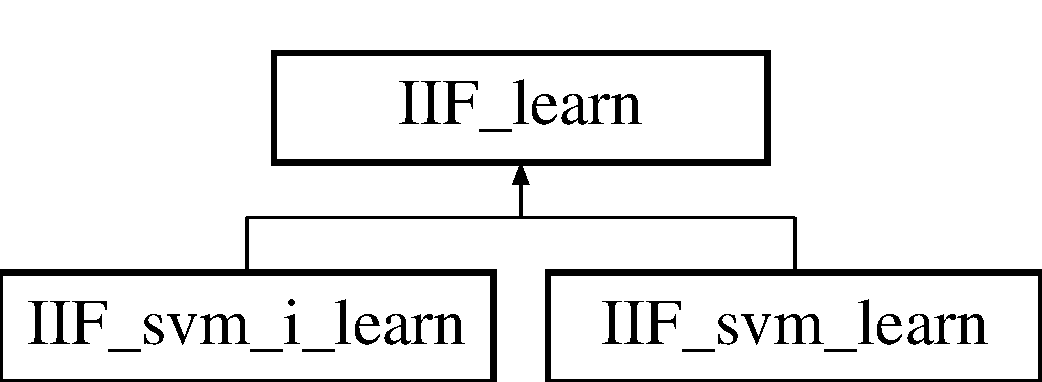
\includegraphics[height=2.000000cm]{classIIF__learn}
\end{center}
\end{figure}
\subsection*{Public Member Functions}
\begin{DoxyCompactItemize}
\item 
\hyperlink{classIIF__learn_a52f7f9a9226409373229a5f9ede446ad}{I\+I\+F\+\_\+learn} (\hyperlink{classStates}{States} $\ast$\hyperlink{classIIF__learn_a2c2157269ef33cd2881ed48c5b38946a}{gsets}, int($\ast$\hyperlink{classIIF__learn_a19119795c6b5360d2e8b3ed2073642d6}{func})(int $\ast$))
\item 
\hyperlink{classIIF__learn_ac0f1fb59ddca48fe5414de299e32730e}{I\+I\+F\+\_\+learn} ()
\item 
void \hyperlink{classIIF__learn_ad91ea13d3761a011d8c75af8e9b54deb}{run\+\_\+target} (\hyperlink{classSolution}{Solution} \&input)
\item 
virtual int \hyperlink{classIIF__learn_aba3602a34e425112a11176c49171dced}{learn} ()=0
\end{DoxyCompactItemize}
\subsection*{Protected Member Functions}
\begin{DoxyCompactItemize}
\item 
void \hyperlink{classIIF__learn_aec195ce429a20cb1503e4f5d1a9bae0e}{init\+\_\+gsets} ()
\end{DoxyCompactItemize}
\subsection*{Protected Attributes}
\begin{DoxyCompactItemize}
\item 
\hyperlink{classStates}{States} $\ast$ \hyperlink{classIIF__learn_a2c2157269ef33cd2881ed48c5b38946a}{gsets}
\item 
int($\ast$ \hyperlink{classIIF__learn_a19119795c6b5360d2e8b3ed2073642d6}{func} )(int $\ast$)
\end{DoxyCompactItemize}


\subsection{Constructor \& Destructor Documentation}
\index{I\+I\+F\+\_\+learn@{I\+I\+F\+\_\+learn}!I\+I\+F\+\_\+learn@{I\+I\+F\+\_\+learn}}
\index{I\+I\+F\+\_\+learn@{I\+I\+F\+\_\+learn}!I\+I\+F\+\_\+learn@{I\+I\+F\+\_\+learn}}
\subsubsection[{I\+I\+F\+\_\+learn(\+States $\ast$gsets, int($\ast$func)(int $\ast$))}]{\setlength{\rightskip}{0pt plus 5cm}I\+I\+F\+\_\+learn\+::\+I\+I\+F\+\_\+learn (
\begin{DoxyParamCaption}
\item[{{\bf States} $\ast$}]{gsets, }
\item[{int($\ast$)(int $\ast$)}]{func}
\end{DoxyParamCaption}
)\hspace{0.3cm}{\ttfamily [inline]}}\hypertarget{classIIF__learn_a52f7f9a9226409373229a5f9ede446ad}{}\label{classIIF__learn_a52f7f9a9226409373229a5f9ede446ad}
\index{I\+I\+F\+\_\+learn@{I\+I\+F\+\_\+learn}!I\+I\+F\+\_\+learn@{I\+I\+F\+\_\+learn}}
\index{I\+I\+F\+\_\+learn@{I\+I\+F\+\_\+learn}!I\+I\+F\+\_\+learn@{I\+I\+F\+\_\+learn}}
\subsubsection[{I\+I\+F\+\_\+learn()}]{\setlength{\rightskip}{0pt plus 5cm}I\+I\+F\+\_\+learn\+::\+I\+I\+F\+\_\+learn (
\begin{DoxyParamCaption}
{}
\end{DoxyParamCaption}
)\hspace{0.3cm}{\ttfamily [inline]}}\hypertarget{classIIF__learn_ac0f1fb59ddca48fe5414de299e32730e}{}\label{classIIF__learn_ac0f1fb59ddca48fe5414de299e32730e}


\subsection{Member Function Documentation}
\index{I\+I\+F\+\_\+learn@{I\+I\+F\+\_\+learn}!init\+\_\+gsets@{init\+\_\+gsets}}
\index{init\+\_\+gsets@{init\+\_\+gsets}!I\+I\+F\+\_\+learn@{I\+I\+F\+\_\+learn}}
\subsubsection[{init\+\_\+gsets()}]{\setlength{\rightskip}{0pt plus 5cm}void I\+I\+F\+\_\+learn\+::init\+\_\+gsets (
\begin{DoxyParamCaption}
{}
\end{DoxyParamCaption}
)\hspace{0.3cm}{\ttfamily [inline]}, {\ttfamily [protected]}}\hypertarget{classIIF__learn_aec195ce429a20cb1503e4f5d1a9bae0e}{}\label{classIIF__learn_aec195ce429a20cb1503e4f5d1a9bae0e}
\index{I\+I\+F\+\_\+learn@{I\+I\+F\+\_\+learn}!learn@{learn}}
\index{learn@{learn}!I\+I\+F\+\_\+learn@{I\+I\+F\+\_\+learn}}
\subsubsection[{learn()=0}]{\setlength{\rightskip}{0pt plus 5cm}virtual int I\+I\+F\+\_\+learn\+::learn (
\begin{DoxyParamCaption}
{}
\end{DoxyParamCaption}
)\hspace{0.3cm}{\ttfamily [pure virtual]}}\hypertarget{classIIF__learn_aba3602a34e425112a11176c49171dced}{}\label{classIIF__learn_aba3602a34e425112a11176c49171dced}


Implemented in \hyperlink{classIIF__svm__i__learn_a054c277c00d749f8eaec0f1eb7156b21}{I\+I\+F\+\_\+svm\+\_\+i\+\_\+learn}, and \hyperlink{classIIF__svm__learn_a5c84275525dbd8140e06f83d33d78b97}{I\+I\+F\+\_\+svm\+\_\+learn}.

\index{I\+I\+F\+\_\+learn@{I\+I\+F\+\_\+learn}!run\+\_\+target@{run\+\_\+target}}
\index{run\+\_\+target@{run\+\_\+target}!I\+I\+F\+\_\+learn@{I\+I\+F\+\_\+learn}}
\subsubsection[{run\+\_\+target(\+Solution \&input)}]{\setlength{\rightskip}{0pt plus 5cm}void I\+I\+F\+\_\+learn\+::run\+\_\+target (
\begin{DoxyParamCaption}
\item[{{\bf Solution} \&}]{input}
\end{DoxyParamCaption}
)\hspace{0.3cm}{\ttfamily [inline]}}\hypertarget{classIIF__learn_ad91ea13d3761a011d8c75af8e9b54deb}{}\label{classIIF__learn_ad91ea13d3761a011d8c75af8e9b54deb}


\subsection{Field Documentation}
\index{I\+I\+F\+\_\+learn@{I\+I\+F\+\_\+learn}!func@{func}}
\index{func@{func}!I\+I\+F\+\_\+learn@{I\+I\+F\+\_\+learn}}
\subsubsection[{func}]{\setlength{\rightskip}{0pt plus 5cm}int($\ast$ I\+I\+F\+\_\+learn\+::func) (int $\ast$)\hspace{0.3cm}{\ttfamily [protected]}}\hypertarget{classIIF__learn_a19119795c6b5360d2e8b3ed2073642d6}{}\label{classIIF__learn_a19119795c6b5360d2e8b3ed2073642d6}
\index{I\+I\+F\+\_\+learn@{I\+I\+F\+\_\+learn}!gsets@{gsets}}
\index{gsets@{gsets}!I\+I\+F\+\_\+learn@{I\+I\+F\+\_\+learn}}
\subsubsection[{gsets}]{\setlength{\rightskip}{0pt plus 5cm}{\bf States}$\ast$ I\+I\+F\+\_\+learn\+::gsets\hspace{0.3cm}{\ttfamily [protected]}}\hypertarget{classIIF__learn_a2c2157269ef33cd2881ed48c5b38946a}{}\label{classIIF__learn_a2c2157269ef33cd2881ed48c5b38946a}


The documentation for this class was generated from the following file\+:\begin{DoxyCompactItemize}
\item 
include/\hyperlink{iif__learn_8h}{iif\+\_\+learn.\+h}\end{DoxyCompactItemize}

\hypertarget{classIIF__svm__i__learn}{}\section{I\+I\+F\+\_\+svm\+\_\+i\+\_\+learn Class Reference}
\label{classIIF__svm__i__learn}\index{I\+I\+F\+\_\+svm\+\_\+i\+\_\+learn@{I\+I\+F\+\_\+svm\+\_\+i\+\_\+learn}}


{\ttfamily \#include $<$iif\+\_\+svm\+\_\+i\+\_\+learn.\+h$>$}

Inheritance diagram for I\+I\+F\+\_\+svm\+\_\+i\+\_\+learn\+:\begin{figure}[H]
\begin{center}
\leavevmode
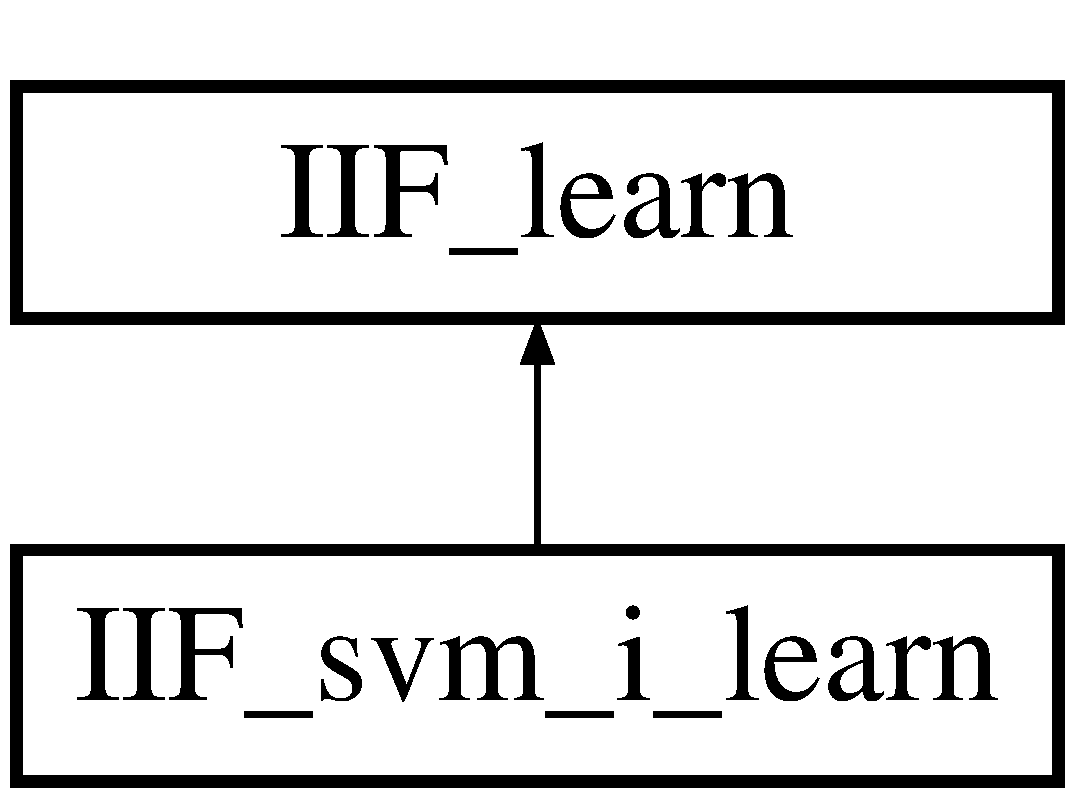
\includegraphics[height=2.000000cm]{classIIF__svm__i__learn}
\end{center}
\end{figure}
\subsection*{Public Member Functions}
\begin{DoxyCompactItemize}
\item 
\hyperlink{classIIF__svm__i__learn_a5a9eece691630be27e994f4300d83fff}{I\+I\+F\+\_\+svm\+\_\+i\+\_\+learn} (\hyperlink{classStates}{States} $\ast$\hyperlink{classIIF__learn_a2c2157269ef33cd2881ed48c5b38946a}{gsets}, int($\ast$\hyperlink{classIIF__learn_a19119795c6b5360d2e8b3ed2073642d6}{func})(int $\ast$), int \hyperlink{classIIF__svm__i__learn_a9beafc489be7aa975aef083ffb1cb270}{max\+\_\+iteration}=\hyperlink{config_8h_a7a2c49f1d0b87e326420efb7e71cb89f}{max\+\_\+iter})
\item 
\hyperlink{classIIF__svm__i__learn_ab1a6ba49ba6018d49477ba2577182b03}{I\+I\+F\+\_\+svm\+\_\+i\+\_\+learn} ()
\item 
virtual int \hyperlink{classIIF__svm__i__learn_a054c277c00d749f8eaec0f1eb7156b21}{learn} ()
\end{DoxyCompactItemize}
\subsection*{Protected Attributes}
\begin{DoxyCompactItemize}
\item 
\hyperlink{classSVM__I}{S\+V\+M\+\_\+I} $\ast$ \hyperlink{classIIF__svm__i__learn_ac9a29f27106b99d511d8ab8dee18831d}{svm\+\_\+i}
\item 
int \hyperlink{classIIF__svm__i__learn_a9beafc489be7aa975aef083ffb1cb270}{max\+\_\+iteration}
\end{DoxyCompactItemize}
\subsection*{Additional Inherited Members}


\subsection{Constructor \& Destructor Documentation}
\index{I\+I\+F\+\_\+svm\+\_\+i\+\_\+learn@{I\+I\+F\+\_\+svm\+\_\+i\+\_\+learn}!I\+I\+F\+\_\+svm\+\_\+i\+\_\+learn@{I\+I\+F\+\_\+svm\+\_\+i\+\_\+learn}}
\index{I\+I\+F\+\_\+svm\+\_\+i\+\_\+learn@{I\+I\+F\+\_\+svm\+\_\+i\+\_\+learn}!I\+I\+F\+\_\+svm\+\_\+i\+\_\+learn@{I\+I\+F\+\_\+svm\+\_\+i\+\_\+learn}}
\subsubsection[{I\+I\+F\+\_\+svm\+\_\+i\+\_\+learn(\+States $\ast$gsets, int($\ast$func)(int $\ast$), int max\+\_\+iteration=max\+\_\+iter)}]{\setlength{\rightskip}{0pt plus 5cm}I\+I\+F\+\_\+svm\+\_\+i\+\_\+learn\+::\+I\+I\+F\+\_\+svm\+\_\+i\+\_\+learn (
\begin{DoxyParamCaption}
\item[{{\bf States} $\ast$}]{gsets, }
\item[{int($\ast$)(int $\ast$)}]{func, }
\item[{int}]{max\+\_\+iteration = {\ttfamily {\bf max\+\_\+iter}}}
\end{DoxyParamCaption}
)}\hypertarget{classIIF__svm__i__learn_a5a9eece691630be27e994f4300d83fff}{}\label{classIIF__svm__i__learn_a5a9eece691630be27e994f4300d83fff}
\index{I\+I\+F\+\_\+svm\+\_\+i\+\_\+learn@{I\+I\+F\+\_\+svm\+\_\+i\+\_\+learn}!I\+I\+F\+\_\+svm\+\_\+i\+\_\+learn@{I\+I\+F\+\_\+svm\+\_\+i\+\_\+learn}}
\index{I\+I\+F\+\_\+svm\+\_\+i\+\_\+learn@{I\+I\+F\+\_\+svm\+\_\+i\+\_\+learn}!I\+I\+F\+\_\+svm\+\_\+i\+\_\+learn@{I\+I\+F\+\_\+svm\+\_\+i\+\_\+learn}}
\subsubsection[{I\+I\+F\+\_\+svm\+\_\+i\+\_\+learn()}]{\setlength{\rightskip}{0pt plus 5cm}I\+I\+F\+\_\+svm\+\_\+i\+\_\+learn\+::\+I\+I\+F\+\_\+svm\+\_\+i\+\_\+learn (
\begin{DoxyParamCaption}
{}
\end{DoxyParamCaption}
)}\hypertarget{classIIF__svm__i__learn_ab1a6ba49ba6018d49477ba2577182b03}{}\label{classIIF__svm__i__learn_ab1a6ba49ba6018d49477ba2577182b03}


\subsection{Member Function Documentation}
\index{I\+I\+F\+\_\+svm\+\_\+i\+\_\+learn@{I\+I\+F\+\_\+svm\+\_\+i\+\_\+learn}!learn@{learn}}
\index{learn@{learn}!I\+I\+F\+\_\+svm\+\_\+i\+\_\+learn@{I\+I\+F\+\_\+svm\+\_\+i\+\_\+learn}}
\subsubsection[{learn()}]{\setlength{\rightskip}{0pt plus 5cm}int I\+I\+F\+\_\+svm\+\_\+i\+\_\+learn\+::learn (
\begin{DoxyParamCaption}
{}
\end{DoxyParamCaption}
)\hspace{0.3cm}{\ttfamily [virtual]}}\hypertarget{classIIF__svm__i__learn_a054c277c00d749f8eaec0f1eb7156b21}{}\label{classIIF__svm__i__learn_a054c277c00d749f8eaec0f1eb7156b21}


Implements \hyperlink{classIIF__learn_aba3602a34e425112a11176c49171dced}{I\+I\+F\+\_\+learn}.



\subsection{Field Documentation}
\index{I\+I\+F\+\_\+svm\+\_\+i\+\_\+learn@{I\+I\+F\+\_\+svm\+\_\+i\+\_\+learn}!max\+\_\+iteration@{max\+\_\+iteration}}
\index{max\+\_\+iteration@{max\+\_\+iteration}!I\+I\+F\+\_\+svm\+\_\+i\+\_\+learn@{I\+I\+F\+\_\+svm\+\_\+i\+\_\+learn}}
\subsubsection[{max\+\_\+iteration}]{\setlength{\rightskip}{0pt plus 5cm}int I\+I\+F\+\_\+svm\+\_\+i\+\_\+learn\+::max\+\_\+iteration\hspace{0.3cm}{\ttfamily [protected]}}\hypertarget{classIIF__svm__i__learn_a9beafc489be7aa975aef083ffb1cb270}{}\label{classIIF__svm__i__learn_a9beafc489be7aa975aef083ffb1cb270}
\index{I\+I\+F\+\_\+svm\+\_\+i\+\_\+learn@{I\+I\+F\+\_\+svm\+\_\+i\+\_\+learn}!svm\+\_\+i@{svm\+\_\+i}}
\index{svm\+\_\+i@{svm\+\_\+i}!I\+I\+F\+\_\+svm\+\_\+i\+\_\+learn@{I\+I\+F\+\_\+svm\+\_\+i\+\_\+learn}}
\subsubsection[{svm\+\_\+i}]{\setlength{\rightskip}{0pt plus 5cm}{\bf S\+V\+M\+\_\+I}$\ast$ I\+I\+F\+\_\+svm\+\_\+i\+\_\+learn\+::svm\+\_\+i\hspace{0.3cm}{\ttfamily [protected]}}\hypertarget{classIIF__svm__i__learn_ac9a29f27106b99d511d8ab8dee18831d}{}\label{classIIF__svm__i__learn_ac9a29f27106b99d511d8ab8dee18831d}


The documentation for this class was generated from the following files\+:\begin{DoxyCompactItemize}
\item 
include/\hyperlink{iif__svm__i__learn_8h}{iif\+\_\+svm\+\_\+i\+\_\+learn.\+h}\item 
src/\hyperlink{iif__svm__i__learn_8cpp}{iif\+\_\+svm\+\_\+i\+\_\+learn.\+cpp}\end{DoxyCompactItemize}

\hypertarget{classIIF__svm__learn}{}\section{I\+I\+F\+\_\+svm\+\_\+learn Class Reference}
\label{classIIF__svm__learn}\index{I\+I\+F\+\_\+svm\+\_\+learn@{I\+I\+F\+\_\+svm\+\_\+learn}}


{\ttfamily \#include $<$iif\+\_\+svm\+\_\+learn.\+h$>$}

Inheritance diagram for I\+I\+F\+\_\+svm\+\_\+learn\+:\begin{figure}[H]
\begin{center}
\leavevmode
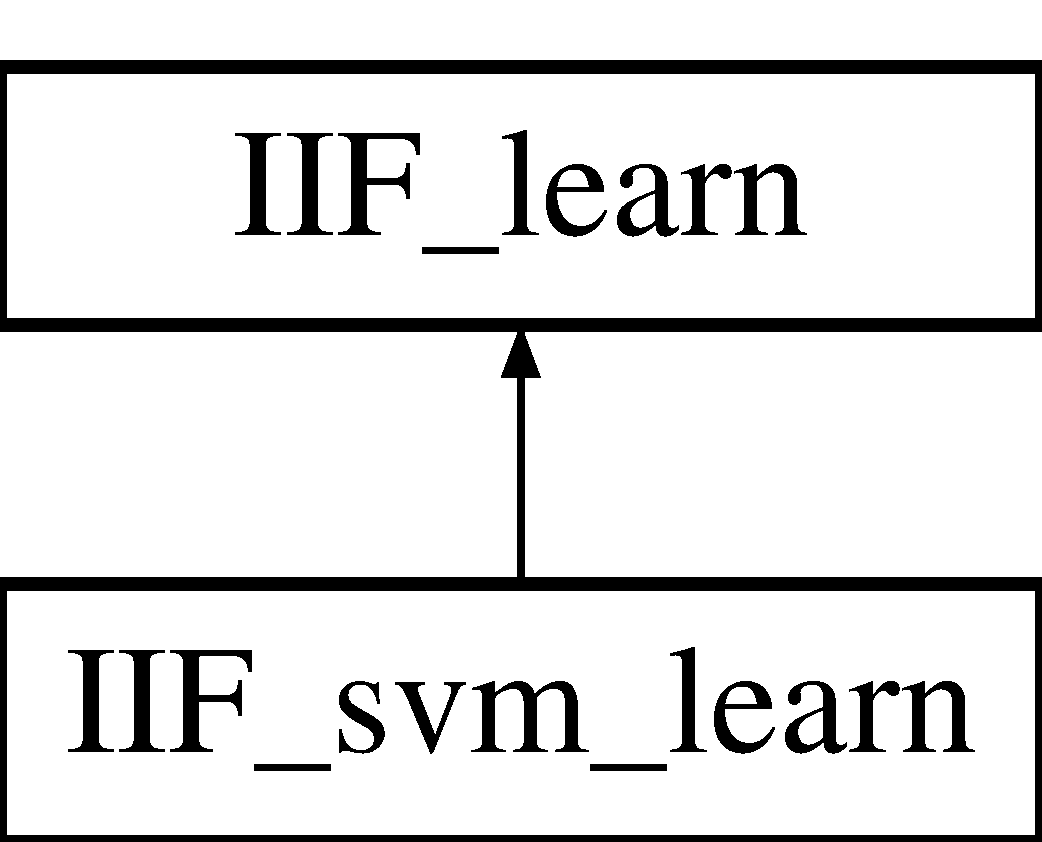
\includegraphics[height=2.000000cm]{classIIF__svm__learn}
\end{center}
\end{figure}
\subsection*{Public Member Functions}
\begin{DoxyCompactItemize}
\item 
\hyperlink{classIIF__svm__learn_a2f7879f8999cb2239f6e06abdb6167c9}{I\+I\+F\+\_\+svm\+\_\+learn} (\hyperlink{classStates}{States} $\ast$\hyperlink{classIIF__learn_a2c2157269ef33cd2881ed48c5b38946a}{gsets}, int($\ast$\hyperlink{classIIF__learn_a19119795c6b5360d2e8b3ed2073642d6}{func})(int $\ast$), int \hyperlink{classIIF__svm__learn_a04b3b7f73edd164462d4923a74189670}{max\+\_\+iteration}=\hyperlink{config_8h_a7a2c49f1d0b87e326420efb7e71cb89f}{max\+\_\+iter})
\item 
\hyperlink{classIIF__svm__learn_a8f6006d617edad515c5f96061843b6cf}{I\+I\+F\+\_\+svm\+\_\+learn} ()
\item 
virtual int \hyperlink{classIIF__svm__learn_a5c84275525dbd8140e06f83d33d78b97}{learn} ()
\end{DoxyCompactItemize}
\subsection*{Protected Attributes}
\begin{DoxyCompactItemize}
\item 
\hyperlink{classSVM}{S\+VM} $\ast$ \hyperlink{classIIF__svm__learn_a0b23f4e2e73ecbdd3755fde75f3c3bc9}{svm}
\item 
int \hyperlink{classIIF__svm__learn_a04b3b7f73edd164462d4923a74189670}{max\+\_\+iteration}
\end{DoxyCompactItemize}
\subsection*{Additional Inherited Members}


\subsection{Constructor \& Destructor Documentation}
\index{I\+I\+F\+\_\+svm\+\_\+learn@{I\+I\+F\+\_\+svm\+\_\+learn}!I\+I\+F\+\_\+svm\+\_\+learn@{I\+I\+F\+\_\+svm\+\_\+learn}}
\index{I\+I\+F\+\_\+svm\+\_\+learn@{I\+I\+F\+\_\+svm\+\_\+learn}!I\+I\+F\+\_\+svm\+\_\+learn@{I\+I\+F\+\_\+svm\+\_\+learn}}
\subsubsection[{I\+I\+F\+\_\+svm\+\_\+learn(\+States $\ast$gsets, int($\ast$func)(int $\ast$), int max\+\_\+iteration=max\+\_\+iter)}]{\setlength{\rightskip}{0pt plus 5cm}I\+I\+F\+\_\+svm\+\_\+learn\+::\+I\+I\+F\+\_\+svm\+\_\+learn (
\begin{DoxyParamCaption}
\item[{{\bf States} $\ast$}]{gsets, }
\item[{int($\ast$)(int $\ast$)}]{func, }
\item[{int}]{max\+\_\+iteration = {\ttfamily {\bf max\+\_\+iter}}}
\end{DoxyParamCaption}
)}\hypertarget{classIIF__svm__learn_a2f7879f8999cb2239f6e06abdb6167c9}{}\label{classIIF__svm__learn_a2f7879f8999cb2239f6e06abdb6167c9}
\index{I\+I\+F\+\_\+svm\+\_\+learn@{I\+I\+F\+\_\+svm\+\_\+learn}!I\+I\+F\+\_\+svm\+\_\+learn@{I\+I\+F\+\_\+svm\+\_\+learn}}
\index{I\+I\+F\+\_\+svm\+\_\+learn@{I\+I\+F\+\_\+svm\+\_\+learn}!I\+I\+F\+\_\+svm\+\_\+learn@{I\+I\+F\+\_\+svm\+\_\+learn}}
\subsubsection[{I\+I\+F\+\_\+svm\+\_\+learn()}]{\setlength{\rightskip}{0pt plus 5cm}I\+I\+F\+\_\+svm\+\_\+learn\+::\+I\+I\+F\+\_\+svm\+\_\+learn (
\begin{DoxyParamCaption}
{}
\end{DoxyParamCaption}
)}\hypertarget{classIIF__svm__learn_a8f6006d617edad515c5f96061843b6cf}{}\label{classIIF__svm__learn_a8f6006d617edad515c5f96061843b6cf}


\subsection{Member Function Documentation}
\index{I\+I\+F\+\_\+svm\+\_\+learn@{I\+I\+F\+\_\+svm\+\_\+learn}!learn@{learn}}
\index{learn@{learn}!I\+I\+F\+\_\+svm\+\_\+learn@{I\+I\+F\+\_\+svm\+\_\+learn}}
\subsubsection[{learn()}]{\setlength{\rightskip}{0pt plus 5cm}int I\+I\+F\+\_\+svm\+\_\+learn\+::learn (
\begin{DoxyParamCaption}
{}
\end{DoxyParamCaption}
)\hspace{0.3cm}{\ttfamily [virtual]}}\hypertarget{classIIF__svm__learn_a5c84275525dbd8140e06f83d33d78b97}{}\label{classIIF__svm__learn_a5c84275525dbd8140e06f83d33d78b97}


Implements \hyperlink{classIIF__learn_aba3602a34e425112a11176c49171dced}{I\+I\+F\+\_\+learn}.



\subsection{Field Documentation}
\index{I\+I\+F\+\_\+svm\+\_\+learn@{I\+I\+F\+\_\+svm\+\_\+learn}!max\+\_\+iteration@{max\+\_\+iteration}}
\index{max\+\_\+iteration@{max\+\_\+iteration}!I\+I\+F\+\_\+svm\+\_\+learn@{I\+I\+F\+\_\+svm\+\_\+learn}}
\subsubsection[{max\+\_\+iteration}]{\setlength{\rightskip}{0pt plus 5cm}int I\+I\+F\+\_\+svm\+\_\+learn\+::max\+\_\+iteration\hspace{0.3cm}{\ttfamily [protected]}}\hypertarget{classIIF__svm__learn_a04b3b7f73edd164462d4923a74189670}{}\label{classIIF__svm__learn_a04b3b7f73edd164462d4923a74189670}
\index{I\+I\+F\+\_\+svm\+\_\+learn@{I\+I\+F\+\_\+svm\+\_\+learn}!svm@{svm}}
\index{svm@{svm}!I\+I\+F\+\_\+svm\+\_\+learn@{I\+I\+F\+\_\+svm\+\_\+learn}}
\subsubsection[{svm}]{\setlength{\rightskip}{0pt plus 5cm}{\bf S\+VM}$\ast$ I\+I\+F\+\_\+svm\+\_\+learn\+::svm\hspace{0.3cm}{\ttfamily [protected]}}\hypertarget{classIIF__svm__learn_a0b23f4e2e73ecbdd3755fde75f3c3bc9}{}\label{classIIF__svm__learn_a0b23f4e2e73ecbdd3755fde75f3c3bc9}


The documentation for this class was generated from the following files\+:\begin{DoxyCompactItemize}
\item 
include/\hyperlink{iif__svm__learn_8h}{iif\+\_\+svm\+\_\+learn.\+h}\item 
src/\hyperlink{iif__svm__learn_8cpp}{iif\+\_\+svm\+\_\+learn.\+cpp}\end{DoxyCompactItemize}

\hypertarget{classKernel}{}\section{Kernel Class Reference}
\label{classKernel}\index{Kernel@{Kernel}}
Inheritance diagram for Kernel\+:\begin{figure}[H]
\begin{center}
\leavevmode
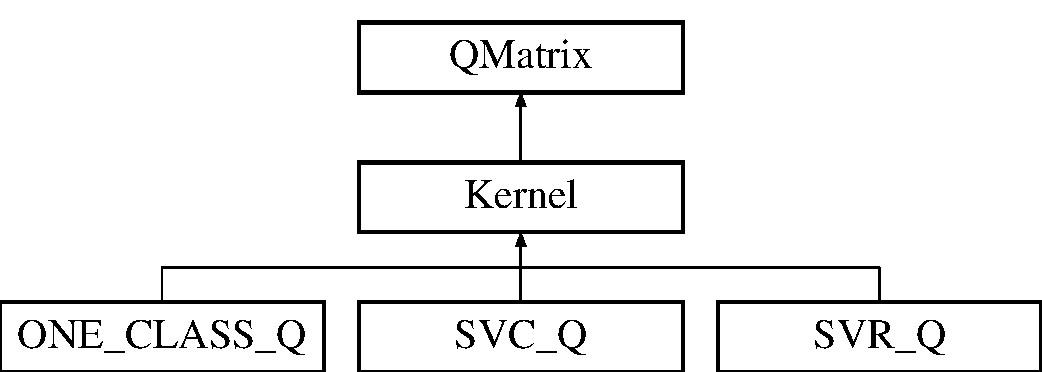
\includegraphics[height=3.000000cm]{classKernel}
\end{center}
\end{figure}
\subsection*{Public Member Functions}
\begin{DoxyCompactItemize}
\item 
\hyperlink{classKernel_a25ffaa0c67cc5b8c7fcdb6f97ca1725f}{Kernel} (int l, \hyperlink{structsvm__node}{svm\+\_\+node} $\ast$const $\ast$x, const \hyperlink{structsvm__parameter}{svm\+\_\+parameter} \&param)
\item 
virtual \hyperlink{classKernel_a9c7407e3a0b1cb9b2f96e9a030187064}{$\sim$\+Kernel} ()
\item 
virtual \hyperlink{svm__core_8cpp_a8755d90a54ecfb8d15051af3e0542592}{Qfloat} $\ast$ \hyperlink{classKernel_a02f328649424359b92b941f5219a6060}{get\+\_\+Q} (int column, int len) const  =0
\item 
virtual double $\ast$ \hyperlink{classKernel_a7bf9602583da1af48d15d19da69514ac}{get\+\_\+\+QD} () const  =0
\item 
virtual void \hyperlink{classKernel_adca807c5584bc42fd098cd9eb1f19621}{swap\+\_\+index} (int i, int j) const 
\end{DoxyCompactItemize}
\subsection*{Static Public Member Functions}
\begin{DoxyCompactItemize}
\item 
static double \hyperlink{classKernel_a6ff0d4ac64bf7fba29d2ca3433dd5127}{k\+\_\+function} (const \hyperlink{structsvm__node}{svm\+\_\+node} $\ast$x, const \hyperlink{structsvm__node}{svm\+\_\+node} $\ast$\hyperlink{untested_2pldi08_8c_a0a2f84ed7838f07779ae24c5a9086d33}{y}, const \hyperlink{structsvm__parameter}{svm\+\_\+parameter} \&param)
\end{DoxyCompactItemize}
\subsection*{Protected Attributes}
\begin{DoxyCompactItemize}
\item 
double(Kernel\+::$\ast$ \hyperlink{classKernel_ac7b39305896e51f9e1a08e026e2c4d9c}{kernel\+\_\+function} )(int i, int j) const 
\end{DoxyCompactItemize}


\subsection{Constructor \& Destructor Documentation}
\index{Kernel@{Kernel}!Kernel@{Kernel}}
\index{Kernel@{Kernel}!Kernel@{Kernel}}
\subsubsection[{Kernel(int l, svm\+\_\+node $\ast$const $\ast$x, const svm\+\_\+parameter \&param)}]{\setlength{\rightskip}{0pt plus 5cm}Kernel\+::\+Kernel (
\begin{DoxyParamCaption}
\item[{int}]{l, }
\item[{{\bf svm\+\_\+node} $\ast$const $\ast$}]{x, }
\item[{const {\bf svm\+\_\+parameter} \&}]{param}
\end{DoxyParamCaption}
)}\hypertarget{classKernel_a25ffaa0c67cc5b8c7fcdb6f97ca1725f}{}\label{classKernel_a25ffaa0c67cc5b8c7fcdb6f97ca1725f}
\index{Kernel@{Kernel}!````~Kernel@{$\sim$\+Kernel}}
\index{````~Kernel@{$\sim$\+Kernel}!Kernel@{Kernel}}
\subsubsection[{$\sim$\+Kernel()}]{\setlength{\rightskip}{0pt plus 5cm}Kernel\+::$\sim$\+Kernel (
\begin{DoxyParamCaption}
{}
\end{DoxyParamCaption}
)\hspace{0.3cm}{\ttfamily [virtual]}}\hypertarget{classKernel_a9c7407e3a0b1cb9b2f96e9a030187064}{}\label{classKernel_a9c7407e3a0b1cb9b2f96e9a030187064}


\subsection{Member Function Documentation}
\index{Kernel@{Kernel}!get\+\_\+Q@{get\+\_\+Q}}
\index{get\+\_\+Q@{get\+\_\+Q}!Kernel@{Kernel}}
\subsubsection[{get\+\_\+\+Q(int column, int len) const  =0}]{\setlength{\rightskip}{0pt plus 5cm}virtual {\bf Qfloat}$\ast$ Kernel\+::get\+\_\+Q (
\begin{DoxyParamCaption}
\item[{int}]{column, }
\item[{int}]{len}
\end{DoxyParamCaption}
) const\hspace{0.3cm}{\ttfamily [pure virtual]}}\hypertarget{classKernel_a02f328649424359b92b941f5219a6060}{}\label{classKernel_a02f328649424359b92b941f5219a6060}


Implements \hyperlink{classQMatrix_aba360e5c50764e2dd013555d20c861f5}{Q\+Matrix}.



Implemented in \hyperlink{classSVR__Q_aba55078d17e7815f093ffa154f3cee9d}{S\+V\+R\+\_\+Q}, \hyperlink{classONE__CLASS__Q_a1f8501234022e017cf46c4dfb2da9d31}{O\+N\+E\+\_\+\+C\+L\+A\+S\+S\+\_\+Q}, and \hyperlink{classSVC__Q_a9341b6030b3fdc88466e4a602b5abff0}{S\+V\+C\+\_\+Q}.

\index{Kernel@{Kernel}!get\+\_\+\+QD@{get\+\_\+\+QD}}
\index{get\+\_\+\+QD@{get\+\_\+\+QD}!Kernel@{Kernel}}
\subsubsection[{get\+\_\+\+Q\+D() const  =0}]{\setlength{\rightskip}{0pt plus 5cm}virtual double$\ast$ Kernel\+::get\+\_\+\+QD (
\begin{DoxyParamCaption}
{}
\end{DoxyParamCaption}
) const\hspace{0.3cm}{\ttfamily [pure virtual]}}\hypertarget{classKernel_a7bf9602583da1af48d15d19da69514ac}{}\label{classKernel_a7bf9602583da1af48d15d19da69514ac}


Implements \hyperlink{classQMatrix_a8fa3bebbb30838d2eef68afdb6da1024}{Q\+Matrix}.



Implemented in \hyperlink{classSVR__Q_ac22ed5ce1b0bf6a900c3c8d631e77d76}{S\+V\+R\+\_\+Q}, \hyperlink{classONE__CLASS__Q_a882480d4370d8a89d667a28c3ed68a73}{O\+N\+E\+\_\+\+C\+L\+A\+S\+S\+\_\+Q}, and \hyperlink{classSVC__Q_ac73020a6e438e209d63223e1fa8cac29}{S\+V\+C\+\_\+Q}.

\index{Kernel@{Kernel}!k\+\_\+function@{k\+\_\+function}}
\index{k\+\_\+function@{k\+\_\+function}!Kernel@{Kernel}}
\subsubsection[{k\+\_\+function(const svm\+\_\+node $\ast$x, const svm\+\_\+node $\ast$y, const svm\+\_\+parameter \&param)}]{\setlength{\rightskip}{0pt plus 5cm}double Kernel\+::k\+\_\+function (
\begin{DoxyParamCaption}
\item[{const {\bf svm\+\_\+node} $\ast$}]{x, }
\item[{const {\bf svm\+\_\+node} $\ast$}]{y, }
\item[{const {\bf svm\+\_\+parameter} \&}]{param}
\end{DoxyParamCaption}
)\hspace{0.3cm}{\ttfamily [static]}}\hypertarget{classKernel_a6ff0d4ac64bf7fba29d2ca3433dd5127}{}\label{classKernel_a6ff0d4ac64bf7fba29d2ca3433dd5127}
\index{Kernel@{Kernel}!swap\+\_\+index@{swap\+\_\+index}}
\index{swap\+\_\+index@{swap\+\_\+index}!Kernel@{Kernel}}
\subsubsection[{swap\+\_\+index(int i, int j) const }]{\setlength{\rightskip}{0pt plus 5cm}virtual void Kernel\+::swap\+\_\+index (
\begin{DoxyParamCaption}
\item[{int}]{i, }
\item[{int}]{j}
\end{DoxyParamCaption}
) const\hspace{0.3cm}{\ttfamily [inline]}, {\ttfamily [virtual]}}\hypertarget{classKernel_adca807c5584bc42fd098cd9eb1f19621}{}\label{classKernel_adca807c5584bc42fd098cd9eb1f19621}


Implements \hyperlink{classQMatrix_a095e38cbf4a02cfb1acc2377f8370628}{Q\+Matrix}.



Reimplemented in \hyperlink{classSVR__Q_a9d3884f0c68f4ce18d47570e4a203405}{S\+V\+R\+\_\+Q}, \hyperlink{classONE__CLASS__Q_ad8bc86ca742c27d82718346388f83fad}{O\+N\+E\+\_\+\+C\+L\+A\+S\+S\+\_\+Q}, and \hyperlink{classSVC__Q_a9c889db8ee0156ed5bcdaa4d6bc4e245}{S\+V\+C\+\_\+Q}.



\subsection{Field Documentation}
\index{Kernel@{Kernel}!kernel\+\_\+function@{kernel\+\_\+function}}
\index{kernel\+\_\+function@{kernel\+\_\+function}!Kernel@{Kernel}}
\subsubsection[{kernel\+\_\+function}]{\setlength{\rightskip}{0pt plus 5cm}double(Kernel\+::$\ast$ Kernel\+::kernel\+\_\+function) (int i, int j) const \hspace{0.3cm}{\ttfamily [protected]}}\hypertarget{classKernel_ac7b39305896e51f9e1a08e026e2c4d9c}{}\label{classKernel_ac7b39305896e51f9e1a08e026e2c4d9c}


The documentation for this class was generated from the following file\+:\begin{DoxyCompactItemize}
\item 
src/\hyperlink{svm__core_8cpp}{svm\+\_\+core.\+cpp}\end{DoxyCompactItemize}

\hypertarget{classML__Algo}{}\section{M\+L\+\_\+\+Algo Class Reference}
\label{classML__Algo}\index{M\+L\+\_\+\+Algo@{M\+L\+\_\+\+Algo}}


{\ttfamily \#include $<$ml\+\_\+algo.\+h$>$}

Inheritance diagram for M\+L\+\_\+\+Algo\+:\begin{figure}[H]
\begin{center}
\leavevmode
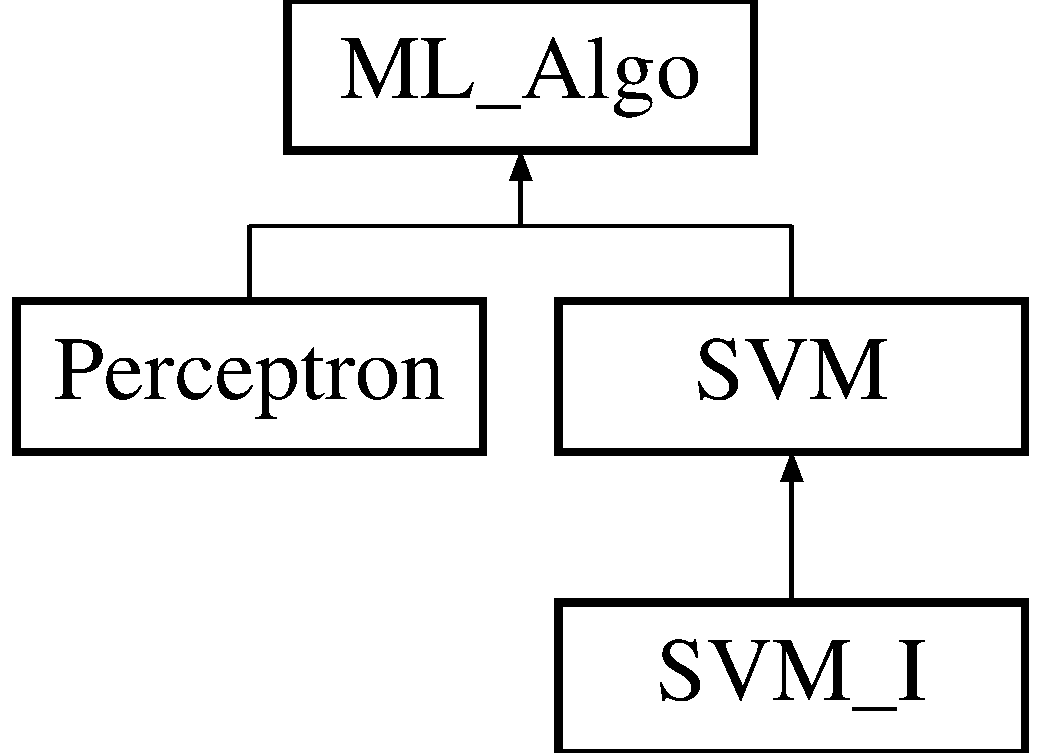
\includegraphics[height=3.000000cm]{classML__Algo}
\end{center}
\end{figure}
\subsection*{Public Member Functions}
\begin{DoxyCompactItemize}
\item 
\hyperlink{classML__Algo_a7b8c13ce9739e50cc6f6d097469f0326}{M\+L\+\_\+\+Algo} ()
\item 
virtual int \hyperlink{classML__Algo_ab98458d234bdf97c2ed678030d90c513}{prepare\+\_\+training\+\_\+data} (\hyperlink{classStates}{States} $\ast$gsets, int \&pre\+\_\+positive\+\_\+size, int \&pre\+\_\+negative\+\_\+size)=0
\begin{DoxyCompactList}\small\item\em init training data method. This should be called before any training happens. \end{DoxyCompactList}\item 
virtual int \hyperlink{classML__Algo_a0a5d241191d4249c60a40d966fb19aee}{train} ()=0
\begin{DoxyCompactList}\small\item\em The most important T\+R\+A\+IN method, which calls real training algorithm to do training. \end{DoxyCompactList}\item 
virtual double \hyperlink{classML__Algo_a39dd640e7c910becf611b9265843ac77}{predict\+\_\+on\+\_\+training\+\_\+set} ()=0
\begin{DoxyCompactList}\small\item\em Calculate the predict precision of the training-\/model on the training set. \end{DoxyCompactList}\item 
virtual int \hyperlink{classML__Algo_a4d757e7fb178ce41ec713bcd84807d33}{check\+\_\+question\+\_\+set} (\hyperlink{classStates}{States} \&qset)=0
\begin{DoxyCompactList}\small\item\em test on question state sets to see if there is an invalidation \end{DoxyCompactList}\item 
virtual int \hyperlink{classML__Algo_a3d2c7bfa53c13005dfde112c9e473c5e}{get\+\_\+converged} (\hyperlink{classEquation}{Equation} $\ast$previous\+\_\+equations, int equation\+\_\+num)=0
\begin{DoxyCompactList}\small\item\em check whether the training is converged or not \end{DoxyCompactList}\item 
virtual std\+::ostream \& \hyperlink{classML__Algo_ad689e5642c5db0971c53909b52cc67d4}{\+\_\+print} (std\+::ostream \&out) const 
\begin{DoxyCompactList}\small\item\em This is the function really called to output this object. We involve this as to support polymophism for operator $<$$<$. \end{DoxyCompactList}\item 
virtual int \hyperlink{classML__Algo_a8650c3894c1992492f8bc86edf1b3ffd}{size} ()=0
\begin{DoxyCompactList}\small\item\em This method returns the current problem size (the number of training states). \end{DoxyCompactList}\item 
virtual \hyperlink{classEquation}{Equation} $\ast$ \hyperlink{classML__Algo_a398214e0462ebfdde10e745240030a34}{roundoff} (int \&equation\+\_\+num)=0
\begin{DoxyCompactList}\small\item\em Round off the whole training model.(equations) \end{DoxyCompactList}\item 
virtual int \hyperlink{classML__Algo_aae12eabc95fd3eb5305f1ae7a14e0193}{predict} (double $\ast$x, int flag)=0
\begin{DoxyCompactList}\small\item\em Predict sample x against the whole training model.(equations) \end{DoxyCompactList}\end{DoxyCompactItemize}
\subsection*{Friends}
\begin{DoxyCompactItemize}
\item 
std\+::ostream \& \hyperlink{classML__Algo_a0d340e61ce196741e6fe74b58f11961c}{operator$<$$<$} (std\+::ostream \&out, const \hyperlink{classML__Algo}{M\+L\+\_\+\+Algo} \&mla)
\begin{DoxyCompactList}\small\item\em output the current trainig result of a \hyperlink{classML__Algo}{M\+L\+\_\+\+Algo} \end{DoxyCompactList}\end{DoxyCompactItemize}


\subsection{Constructor \& Destructor Documentation}
\index{M\+L\+\_\+\+Algo@{M\+L\+\_\+\+Algo}!M\+L\+\_\+\+Algo@{M\+L\+\_\+\+Algo}}
\index{M\+L\+\_\+\+Algo@{M\+L\+\_\+\+Algo}!M\+L\+\_\+\+Algo@{M\+L\+\_\+\+Algo}}
\subsubsection[{M\+L\+\_\+\+Algo()}]{\setlength{\rightskip}{0pt plus 5cm}M\+L\+\_\+\+Algo\+::\+M\+L\+\_\+\+Algo (
\begin{DoxyParamCaption}
{}
\end{DoxyParamCaption}
)\hspace{0.3cm}{\ttfamily [inline]}}\hypertarget{classML__Algo_a7b8c13ce9739e50cc6f6d097469f0326}{}\label{classML__Algo_a7b8c13ce9739e50cc6f6d097469f0326}


\subsection{Member Function Documentation}
\index{M\+L\+\_\+\+Algo@{M\+L\+\_\+\+Algo}!\+\_\+print@{\+\_\+print}}
\index{\+\_\+print@{\+\_\+print}!M\+L\+\_\+\+Algo@{M\+L\+\_\+\+Algo}}
\subsubsection[{\+\_\+print(std\+::ostream \&out) const }]{\setlength{\rightskip}{0pt plus 5cm}virtual std\+::ostream\& M\+L\+\_\+\+Algo\+::\+\_\+print (
\begin{DoxyParamCaption}
\item[{std\+::ostream \&}]{out}
\end{DoxyParamCaption}
) const\hspace{0.3cm}{\ttfamily [inline]}, {\ttfamily [virtual]}}\hypertarget{classML__Algo_ad689e5642c5db0971c53909b52cc67d4}{}\label{classML__Algo_ad689e5642c5db0971c53909b52cc67d4}


This is the function really called to output this object. We involve this as to support polymophism for operator $<$$<$. 



Reimplemented in \hyperlink{classSVM__I_ab0ae30d86d9f9026908a7b902f7a78e3}{S\+V\+M\+\_\+I}, and \hyperlink{classSVM_a6e5a3fbae4da1ecd4773173a2b590c21}{S\+VM}.

\index{M\+L\+\_\+\+Algo@{M\+L\+\_\+\+Algo}!check\+\_\+question\+\_\+set@{check\+\_\+question\+\_\+set}}
\index{check\+\_\+question\+\_\+set@{check\+\_\+question\+\_\+set}!M\+L\+\_\+\+Algo@{M\+L\+\_\+\+Algo}}
\subsubsection[{check\+\_\+question\+\_\+set(\+States \&qset)=0}]{\setlength{\rightskip}{0pt plus 5cm}virtual int M\+L\+\_\+\+Algo\+::check\+\_\+question\+\_\+set (
\begin{DoxyParamCaption}
\item[{{\bf States} \&}]{qset}
\end{DoxyParamCaption}
)\hspace{0.3cm}{\ttfamily [pure virtual]}}\hypertarget{classML__Algo_a4d757e7fb178ce41ec713bcd84807d33}{}\label{classML__Algo_a4d757e7fb178ce41ec713bcd84807d33}


test on question state sets to see if there is an invalidation 

The method will output the inforamtion if a question trace invalidate the training model


\begin{DoxyParams}{Parameters}
{\em qset} & is a reference type to question states. \\
\hline
\end{DoxyParams}
\begin{DoxyReturn}{Returns}
int 0 if no error 
\end{DoxyReturn}


Implemented in \hyperlink{classSVM__I_a84470dce77add6377454c4408c6c1466}{S\+V\+M\+\_\+I}, \hyperlink{classPerceptron_ac7ed76c6a28180691f63f2afbf93cc26}{Perceptron}, and \hyperlink{classSVM_aa610ec08173c8603ad6e02f26cbe8e1c}{S\+VM}.

\index{M\+L\+\_\+\+Algo@{M\+L\+\_\+\+Algo}!get\+\_\+converged@{get\+\_\+converged}}
\index{get\+\_\+converged@{get\+\_\+converged}!M\+L\+\_\+\+Algo@{M\+L\+\_\+\+Algo}}
\subsubsection[{get\+\_\+converged(\+Equation $\ast$previous\+\_\+equations, int equation\+\_\+num)=0}]{\setlength{\rightskip}{0pt plus 5cm}virtual int M\+L\+\_\+\+Algo\+::get\+\_\+converged (
\begin{DoxyParamCaption}
\item[{{\bf Equation} $\ast$}]{previous\+\_\+equations, }
\item[{int}]{equation\+\_\+num}
\end{DoxyParamCaption}
)\hspace{0.3cm}{\ttfamily [pure virtual]}}\hypertarget{classML__Algo_a3d2c7bfa53c13005dfde112c9e473c5e}{}\label{classML__Algo_a3d2c7bfa53c13005dfde112c9e473c5e}


check whether the training is converged or not 

current\+\_\+training\+\_\+equations $\sim$= previous\+\_\+trainig\+\_\+equations ???


\begin{DoxyParams}{Parameters}
{\em previous\+\_\+equations} & contains all the equation we get from last trainig session. \\
\hline
{\em equation\+\_\+num} & is the number of equations get from last training session \\
\hline
\end{DoxyParams}
\begin{DoxyReturn}{Returns}
int 0 if converged 
\end{DoxyReturn}


Implemented in \hyperlink{classSVM__I_a5d1a8c93d41597aea5f31689687dbc77}{S\+V\+M\+\_\+I}, and \hyperlink{classSVM_a712dcd7cb65a8045a77dd474869dd5c4}{S\+VM}.

\index{M\+L\+\_\+\+Algo@{M\+L\+\_\+\+Algo}!predict@{predict}}
\index{predict@{predict}!M\+L\+\_\+\+Algo@{M\+L\+\_\+\+Algo}}
\subsubsection[{predict(double $\ast$x, int flag)=0}]{\setlength{\rightskip}{0pt plus 5cm}virtual int M\+L\+\_\+\+Algo\+::predict (
\begin{DoxyParamCaption}
\item[{double $\ast$}]{x, }
\item[{int}]{flag}
\end{DoxyParamCaption}
)\hspace{0.3cm}{\ttfamily [pure virtual]}}\hypertarget{classML__Algo_aae12eabc95fd3eb5305f1ae7a14e0193}{}\label{classML__Algo_aae12eabc95fd3eb5305f1ae7a14e0193}


Predict sample x against the whole training model.(equations) 


\begin{DoxyParams}{Parameters}
{\em x} & contains the sample to be tested. \\
\hline
{\em flag} & leave this to be Z\+E\+RO... \\
\hline
\end{DoxyParams}
\begin{DoxyReturn}{Returns}
The label of prediction 
\end{DoxyReturn}


Implemented in \hyperlink{classSVM__I_abe0a76aa6d31d18c2ee66002c35c813f}{S\+V\+M\+\_\+I}, \hyperlink{classSVM_a972215d3c749ba550c85763c8871567f}{S\+VM}, and \hyperlink{classPerceptron_a414600a1f189c4f44c858b87048ae655}{Perceptron}.

\index{M\+L\+\_\+\+Algo@{M\+L\+\_\+\+Algo}!predict\+\_\+on\+\_\+training\+\_\+set@{predict\+\_\+on\+\_\+training\+\_\+set}}
\index{predict\+\_\+on\+\_\+training\+\_\+set@{predict\+\_\+on\+\_\+training\+\_\+set}!M\+L\+\_\+\+Algo@{M\+L\+\_\+\+Algo}}
\subsubsection[{predict\+\_\+on\+\_\+training\+\_\+set()=0}]{\setlength{\rightskip}{0pt plus 5cm}virtual double M\+L\+\_\+\+Algo\+::predict\+\_\+on\+\_\+training\+\_\+set (
\begin{DoxyParamCaption}
{}
\end{DoxyParamCaption}
)\hspace{0.3cm}{\ttfamily [pure virtual]}}\hypertarget{classML__Algo_a39dd640e7c910becf611b9265843ac77}{}\label{classML__Algo_a39dd640e7c910becf611b9265843ac77}


Calculate the predict precision of the training-\/model on the training set. 

\begin{DoxyReturn}{Returns}
double Return precision we can get. Should be a value between 0 and 1. 
\end{DoxyReturn}


Implemented in \hyperlink{classSVM__I_a643c2a6e58f8e70ab276ade9b1873bf6}{S\+V\+M\+\_\+I}, \hyperlink{classPerceptron_ac9214d2cda4eeb9a06f6562bcb5df8ca}{Perceptron}, and \hyperlink{classSVM_af208fc653a382591f20c0fcf7a186362}{S\+VM}.

\index{M\+L\+\_\+\+Algo@{M\+L\+\_\+\+Algo}!prepare\+\_\+training\+\_\+data@{prepare\+\_\+training\+\_\+data}}
\index{prepare\+\_\+training\+\_\+data@{prepare\+\_\+training\+\_\+data}!M\+L\+\_\+\+Algo@{M\+L\+\_\+\+Algo}}
\subsubsection[{prepare\+\_\+training\+\_\+data(\+States $\ast$gsets, int \&pre\+\_\+positive\+\_\+size, int \&pre\+\_\+negative\+\_\+size)=0}]{\setlength{\rightskip}{0pt plus 5cm}virtual int M\+L\+\_\+\+Algo\+::prepare\+\_\+training\+\_\+data (
\begin{DoxyParamCaption}
\item[{{\bf States} $\ast$}]{gsets, }
\item[{int \&}]{pre\+\_\+positive\+\_\+size, }
\item[{int \&}]{pre\+\_\+negative\+\_\+size}
\end{DoxyParamCaption}
)\hspace{0.3cm}{\ttfamily [pure virtual]}}\hypertarget{classML__Algo_ab98458d234bdf97c2ed678030d90c513}{}\label{classML__Algo_ab98458d234bdf97c2ed678030d90c513}


init training data method. This should be called before any training happens. 


\begin{DoxyParams}{Parameters}
{\em gsets} & The states array to store all the generated states information. The size must be 4, and index -\/1 should be accessible \\
\hline
{\em pre\+\_\+positive\+\_\+size} & This records the last positive size of states. And also set by callee to the new value Initially set to 0, as there is no elements in positive states. Calls afterwards should pass the value set by last call. \\
\hline
{\em pre\+\_\+negative\+\_\+size} & This records the last negative size of states. And also set by callee to the new value Initially set to 0, as there is no elements in positive states. Calls afterwards should pass the value set by last call. \\
\hline
\end{DoxyParams}
\begin{DoxyReturn}{Returns}
int 0 if no error 
\end{DoxyReturn}


Implemented in \hyperlink{classSVM__I_ab0236699daa4967cfec71234faa785c5}{S\+V\+M\+\_\+I}, \hyperlink{classPerceptron_a2267c5acf9b4a7bd0f47522a530d3863}{Perceptron}, and \hyperlink{classSVM_a930fe217e3affd64acb6700f5f8082e1}{S\+VM}.

\index{M\+L\+\_\+\+Algo@{M\+L\+\_\+\+Algo}!roundoff@{roundoff}}
\index{roundoff@{roundoff}!M\+L\+\_\+\+Algo@{M\+L\+\_\+\+Algo}}
\subsubsection[{roundoff(int \&equation\+\_\+num)=0}]{\setlength{\rightskip}{0pt plus 5cm}virtual {\bf Equation}$\ast$ M\+L\+\_\+\+Algo\+::roundoff (
\begin{DoxyParamCaption}
\item[{int \&}]{equation\+\_\+num}
\end{DoxyParamCaption}
)\hspace{0.3cm}{\ttfamily [pure virtual]}}\hypertarget{classML__Algo_a398214e0462ebfdde10e745240030a34}{}\label{classML__Algo_a398214e0462ebfdde10e745240030a34}


Round off the whole training model.(equations) 


\begin{DoxyParams}{Parameters}
{\em equation\+\_\+num} & set by callee to notify the number of equations we currently get \\
\hline
\end{DoxyParams}
\begin{DoxyReturn}{Returns}
Eqation Point the rounded off equations. Remember to D\+E\+L\+E\+TE them after use by caller. Otherwise memory leak. 
\end{DoxyReturn}


Implemented in \hyperlink{classSVM__I_a91b713ef0810fd4c83a5c711aea9fecf}{S\+V\+M\+\_\+I}, \hyperlink{classSVM_abd2d511c6cb9f64a29a4551f6435bfd2}{S\+VM}, and \hyperlink{classPerceptron_a5408f0ea545d06bbef6630071c73fea2}{Perceptron}.

\index{M\+L\+\_\+\+Algo@{M\+L\+\_\+\+Algo}!size@{size}}
\index{size@{size}!M\+L\+\_\+\+Algo@{M\+L\+\_\+\+Algo}}
\subsubsection[{size()=0}]{\setlength{\rightskip}{0pt plus 5cm}virtual int M\+L\+\_\+\+Algo\+::size (
\begin{DoxyParamCaption}
{}
\end{DoxyParamCaption}
)\hspace{0.3cm}{\ttfamily [pure virtual]}}\hypertarget{classML__Algo_a8650c3894c1992492f8bc86edf1b3ffd}{}\label{classML__Algo_a8650c3894c1992492f8bc86edf1b3ffd}


This method returns the current problem size (the number of training states). 

\begin{DoxyReturn}{Returns}
int the size of problem 
\end{DoxyReturn}


Implemented in \hyperlink{classSVM__I_a1b66cefe313cffaa77d4271dfb4b8474}{S\+V\+M\+\_\+I}, \hyperlink{classSVM_a4563cef982f6e1c67acf0c7b0ec8909b}{S\+VM}, and \hyperlink{classPerceptron_a50b1f76eb2760b540477135100dcbf49}{Perceptron}.

\index{M\+L\+\_\+\+Algo@{M\+L\+\_\+\+Algo}!train@{train}}
\index{train@{train}!M\+L\+\_\+\+Algo@{M\+L\+\_\+\+Algo}}
\subsubsection[{train()=0}]{\setlength{\rightskip}{0pt plus 5cm}virtual int M\+L\+\_\+\+Algo\+::train (
\begin{DoxyParamCaption}
{}
\end{DoxyParamCaption}
)\hspace{0.3cm}{\ttfamily [pure virtual]}}\hypertarget{classML__Algo_a0a5d241191d4249c60a40d966fb19aee}{}\label{classML__Algo_a0a5d241191d4249c60a40d966fb19aee}


The most important T\+R\+A\+IN method, which calls real training algorithm to do training. 

\begin{DoxyReturn}{Returns}
int 0 if no error. 
\end{DoxyReturn}


Implemented in \hyperlink{classSVM__I_abf732821c264b2cb8bef5d252991f2b6}{S\+V\+M\+\_\+I}, \hyperlink{classPerceptron_adc779991ee63dca333c12fb247b32c9d}{Perceptron}, and \hyperlink{classSVM_a6a1d895b86522eab683d66ded4d3a049}{S\+VM}.



\subsection{Friends And Related Function Documentation}
\index{M\+L\+\_\+\+Algo@{M\+L\+\_\+\+Algo}!operator$<$$<$@{operator$<$$<$}}
\index{operator$<$$<$@{operator$<$$<$}!M\+L\+\_\+\+Algo@{M\+L\+\_\+\+Algo}}
\subsubsection[{operator$<$$<$}]{\setlength{\rightskip}{0pt plus 5cm}std\+::ostream\& operator$<$$<$ (
\begin{DoxyParamCaption}
\item[{std\+::ostream \&}]{out, }
\item[{const {\bf M\+L\+\_\+\+Algo} \&}]{mla}
\end{DoxyParamCaption}
)\hspace{0.3cm}{\ttfamily [friend]}}\hypertarget{classML__Algo_a0d340e61ce196741e6fe74b58f11961c}{}\label{classML__Algo_a0d340e61ce196741e6fe74b58f11961c}


output the current trainig result of a \hyperlink{classML__Algo}{M\+L\+\_\+\+Algo} 


\begin{DoxyParams}{Parameters}
{\em mla} & the ml\+\_\+algo object to be output \\
\hline
\end{DoxyParams}
\begin{DoxyReturn}{Returns}
std\+::ostream 
\end{DoxyReturn}


The documentation for this class was generated from the following file\+:\begin{DoxyCompactItemize}
\item 
include/\hyperlink{ml__algo_8h}{ml\+\_\+algo.\+h}\end{DoxyCompactItemize}

\hypertarget{classONE__CLASS__Q}{}\section{O\+N\+E\+\_\+\+C\+L\+A\+S\+S\+\_\+Q Class Reference}
\label{classONE__CLASS__Q}\index{O\+N\+E\+\_\+\+C\+L\+A\+S\+S\+\_\+Q@{O\+N\+E\+\_\+\+C\+L\+A\+S\+S\+\_\+Q}}
Inheritance diagram for O\+N\+E\+\_\+\+C\+L\+A\+S\+S\+\_\+Q\+:\begin{figure}[H]
\begin{center}
\leavevmode
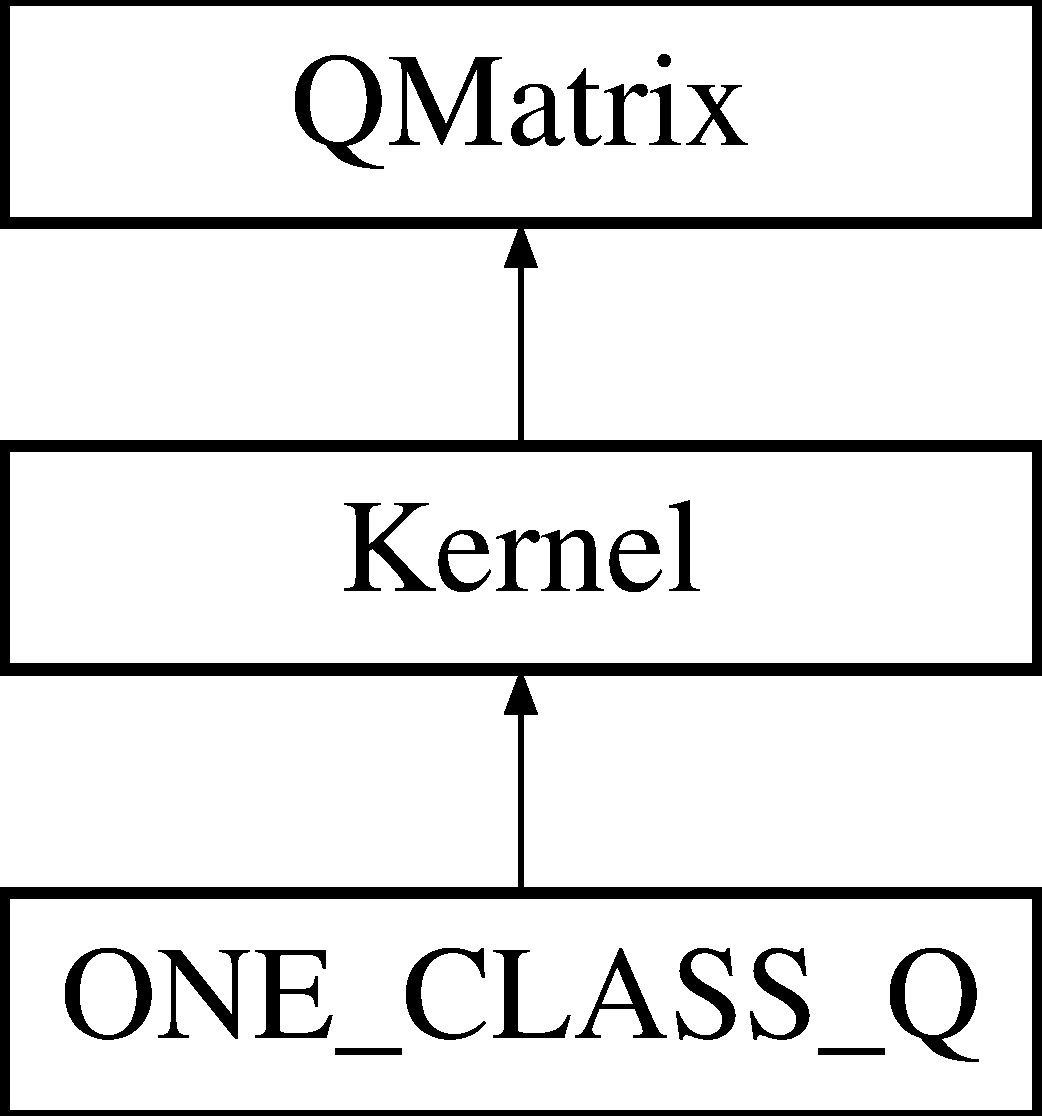
\includegraphics[height=3.000000cm]{classONE__CLASS__Q}
\end{center}
\end{figure}
\subsection*{Public Member Functions}
\begin{DoxyCompactItemize}
\item 
\hyperlink{classONE__CLASS__Q_a759ec4e3e00887ed848cf3f79ab7065f}{O\+N\+E\+\_\+\+C\+L\+A\+S\+S\+\_\+Q} (const \hyperlink{structsvm__problem}{svm\+\_\+problem} \&prob, const \hyperlink{structsvm__parameter}{svm\+\_\+parameter} \&param)
\item 
\hyperlink{svm__core_8cpp_a8755d90a54ecfb8d15051af3e0542592}{Qfloat} $\ast$ \hyperlink{classONE__CLASS__Q_a1f8501234022e017cf46c4dfb2da9d31}{get\+\_\+Q} (int i, int len) const 
\item 
double $\ast$ \hyperlink{classONE__CLASS__Q_a882480d4370d8a89d667a28c3ed68a73}{get\+\_\+\+QD} () const 
\item 
void \hyperlink{classONE__CLASS__Q_ad8bc86ca742c27d82718346388f83fad}{swap\+\_\+index} (int i, int j) const 
\item 
\hyperlink{classONE__CLASS__Q_a569ea8969478398736d70eacc84edbad}{$\sim$\+O\+N\+E\+\_\+\+C\+L\+A\+S\+S\+\_\+Q} ()
\end{DoxyCompactItemize}
\subsection*{Private Attributes}
\begin{DoxyCompactItemize}
\item 
\hyperlink{classCache}{Cache} $\ast$ \hyperlink{classONE__CLASS__Q_ac9b44c80098f3dfb45b1119b9db50907}{cache}
\item 
double $\ast$ \hyperlink{classONE__CLASS__Q_a12994904e59c98ac7f7ec964ea23b7b4}{QD}
\end{DoxyCompactItemize}
\subsection*{Additional Inherited Members}


\subsection{Constructor \& Destructor Documentation}
\index{O\+N\+E\+\_\+\+C\+L\+A\+S\+S\+\_\+Q@{O\+N\+E\+\_\+\+C\+L\+A\+S\+S\+\_\+Q}!O\+N\+E\+\_\+\+C\+L\+A\+S\+S\+\_\+Q@{O\+N\+E\+\_\+\+C\+L\+A\+S\+S\+\_\+Q}}
\index{O\+N\+E\+\_\+\+C\+L\+A\+S\+S\+\_\+Q@{O\+N\+E\+\_\+\+C\+L\+A\+S\+S\+\_\+Q}!O\+N\+E\+\_\+\+C\+L\+A\+S\+S\+\_\+Q@{O\+N\+E\+\_\+\+C\+L\+A\+S\+S\+\_\+Q}}
\subsubsection[{O\+N\+E\+\_\+\+C\+L\+A\+S\+S\+\_\+\+Q(const svm\+\_\+problem \&prob, const svm\+\_\+parameter \&param)}]{\setlength{\rightskip}{0pt plus 5cm}O\+N\+E\+\_\+\+C\+L\+A\+S\+S\+\_\+\+Q\+::\+O\+N\+E\+\_\+\+C\+L\+A\+S\+S\+\_\+Q (
\begin{DoxyParamCaption}
\item[{const {\bf svm\+\_\+problem} \&}]{prob, }
\item[{const {\bf svm\+\_\+parameter} \&}]{param}
\end{DoxyParamCaption}
)\hspace{0.3cm}{\ttfamily [inline]}}\hypertarget{classONE__CLASS__Q_a759ec4e3e00887ed848cf3f79ab7065f}{}\label{classONE__CLASS__Q_a759ec4e3e00887ed848cf3f79ab7065f}
\index{O\+N\+E\+\_\+\+C\+L\+A\+S\+S\+\_\+Q@{O\+N\+E\+\_\+\+C\+L\+A\+S\+S\+\_\+Q}!````~O\+N\+E\+\_\+\+C\+L\+A\+S\+S\+\_\+Q@{$\sim$\+O\+N\+E\+\_\+\+C\+L\+A\+S\+S\+\_\+Q}}
\index{````~O\+N\+E\+\_\+\+C\+L\+A\+S\+S\+\_\+Q@{$\sim$\+O\+N\+E\+\_\+\+C\+L\+A\+S\+S\+\_\+Q}!O\+N\+E\+\_\+\+C\+L\+A\+S\+S\+\_\+Q@{O\+N\+E\+\_\+\+C\+L\+A\+S\+S\+\_\+Q}}
\subsubsection[{$\sim$\+O\+N\+E\+\_\+\+C\+L\+A\+S\+S\+\_\+\+Q()}]{\setlength{\rightskip}{0pt plus 5cm}O\+N\+E\+\_\+\+C\+L\+A\+S\+S\+\_\+\+Q\+::$\sim$\+O\+N\+E\+\_\+\+C\+L\+A\+S\+S\+\_\+Q (
\begin{DoxyParamCaption}
{}
\end{DoxyParamCaption}
)\hspace{0.3cm}{\ttfamily [inline]}}\hypertarget{classONE__CLASS__Q_a569ea8969478398736d70eacc84edbad}{}\label{classONE__CLASS__Q_a569ea8969478398736d70eacc84edbad}


\subsection{Member Function Documentation}
\index{O\+N\+E\+\_\+\+C\+L\+A\+S\+S\+\_\+Q@{O\+N\+E\+\_\+\+C\+L\+A\+S\+S\+\_\+Q}!get\+\_\+Q@{get\+\_\+Q}}
\index{get\+\_\+Q@{get\+\_\+Q}!O\+N\+E\+\_\+\+C\+L\+A\+S\+S\+\_\+Q@{O\+N\+E\+\_\+\+C\+L\+A\+S\+S\+\_\+Q}}
\subsubsection[{get\+\_\+\+Q(int i, int len) const }]{\setlength{\rightskip}{0pt plus 5cm}{\bf Qfloat}$\ast$ O\+N\+E\+\_\+\+C\+L\+A\+S\+S\+\_\+\+Q\+::get\+\_\+Q (
\begin{DoxyParamCaption}
\item[{int}]{i, }
\item[{int}]{len}
\end{DoxyParamCaption}
) const\hspace{0.3cm}{\ttfamily [inline]}, {\ttfamily [virtual]}}\hypertarget{classONE__CLASS__Q_a1f8501234022e017cf46c4dfb2da9d31}{}\label{classONE__CLASS__Q_a1f8501234022e017cf46c4dfb2da9d31}


Implements \hyperlink{classKernel_a02f328649424359b92b941f5219a6060}{Kernel}.

\index{O\+N\+E\+\_\+\+C\+L\+A\+S\+S\+\_\+Q@{O\+N\+E\+\_\+\+C\+L\+A\+S\+S\+\_\+Q}!get\+\_\+\+QD@{get\+\_\+\+QD}}
\index{get\+\_\+\+QD@{get\+\_\+\+QD}!O\+N\+E\+\_\+\+C\+L\+A\+S\+S\+\_\+Q@{O\+N\+E\+\_\+\+C\+L\+A\+S\+S\+\_\+Q}}
\subsubsection[{get\+\_\+\+Q\+D() const }]{\setlength{\rightskip}{0pt plus 5cm}double$\ast$ O\+N\+E\+\_\+\+C\+L\+A\+S\+S\+\_\+\+Q\+::get\+\_\+\+QD (
\begin{DoxyParamCaption}
{}
\end{DoxyParamCaption}
) const\hspace{0.3cm}{\ttfamily [inline]}, {\ttfamily [virtual]}}\hypertarget{classONE__CLASS__Q_a882480d4370d8a89d667a28c3ed68a73}{}\label{classONE__CLASS__Q_a882480d4370d8a89d667a28c3ed68a73}


Implements \hyperlink{classKernel_a7bf9602583da1af48d15d19da69514ac}{Kernel}.

\index{O\+N\+E\+\_\+\+C\+L\+A\+S\+S\+\_\+Q@{O\+N\+E\+\_\+\+C\+L\+A\+S\+S\+\_\+Q}!swap\+\_\+index@{swap\+\_\+index}}
\index{swap\+\_\+index@{swap\+\_\+index}!O\+N\+E\+\_\+\+C\+L\+A\+S\+S\+\_\+Q@{O\+N\+E\+\_\+\+C\+L\+A\+S\+S\+\_\+Q}}
\subsubsection[{swap\+\_\+index(int i, int j) const }]{\setlength{\rightskip}{0pt plus 5cm}void O\+N\+E\+\_\+\+C\+L\+A\+S\+S\+\_\+\+Q\+::swap\+\_\+index (
\begin{DoxyParamCaption}
\item[{int}]{i, }
\item[{int}]{j}
\end{DoxyParamCaption}
) const\hspace{0.3cm}{\ttfamily [inline]}, {\ttfamily [virtual]}}\hypertarget{classONE__CLASS__Q_ad8bc86ca742c27d82718346388f83fad}{}\label{classONE__CLASS__Q_ad8bc86ca742c27d82718346388f83fad}


Reimplemented from \hyperlink{classKernel_adca807c5584bc42fd098cd9eb1f19621}{Kernel}.



\subsection{Field Documentation}
\index{O\+N\+E\+\_\+\+C\+L\+A\+S\+S\+\_\+Q@{O\+N\+E\+\_\+\+C\+L\+A\+S\+S\+\_\+Q}!cache@{cache}}
\index{cache@{cache}!O\+N\+E\+\_\+\+C\+L\+A\+S\+S\+\_\+Q@{O\+N\+E\+\_\+\+C\+L\+A\+S\+S\+\_\+Q}}
\subsubsection[{cache}]{\setlength{\rightskip}{0pt plus 5cm}{\bf Cache}$\ast$ O\+N\+E\+\_\+\+C\+L\+A\+S\+S\+\_\+\+Q\+::cache\hspace{0.3cm}{\ttfamily [private]}}\hypertarget{classONE__CLASS__Q_ac9b44c80098f3dfb45b1119b9db50907}{}\label{classONE__CLASS__Q_ac9b44c80098f3dfb45b1119b9db50907}
\index{O\+N\+E\+\_\+\+C\+L\+A\+S\+S\+\_\+Q@{O\+N\+E\+\_\+\+C\+L\+A\+S\+S\+\_\+Q}!QD@{QD}}
\index{QD@{QD}!O\+N\+E\+\_\+\+C\+L\+A\+S\+S\+\_\+Q@{O\+N\+E\+\_\+\+C\+L\+A\+S\+S\+\_\+Q}}
\subsubsection[{QD}]{\setlength{\rightskip}{0pt plus 5cm}double$\ast$ O\+N\+E\+\_\+\+C\+L\+A\+S\+S\+\_\+\+Q\+::\+QD\hspace{0.3cm}{\ttfamily [private]}}\hypertarget{classONE__CLASS__Q_a12994904e59c98ac7f7ec964ea23b7b4}{}\label{classONE__CLASS__Q_a12994904e59c98ac7f7ec964ea23b7b4}


The documentation for this class was generated from the following file\+:\begin{DoxyCompactItemize}
\item 
src/\hyperlink{svm__core_8cpp}{svm\+\_\+core.\+cpp}\end{DoxyCompactItemize}

\hypertarget{classPerceptron}{}\section{Perceptron Class Reference}
\label{classPerceptron}\index{Perceptron@{Perceptron}}


{\ttfamily \#include $<$perceptron.\+h$>$}

Inheritance diagram for Perceptron\+:\begin{figure}[H]
\begin{center}
\leavevmode
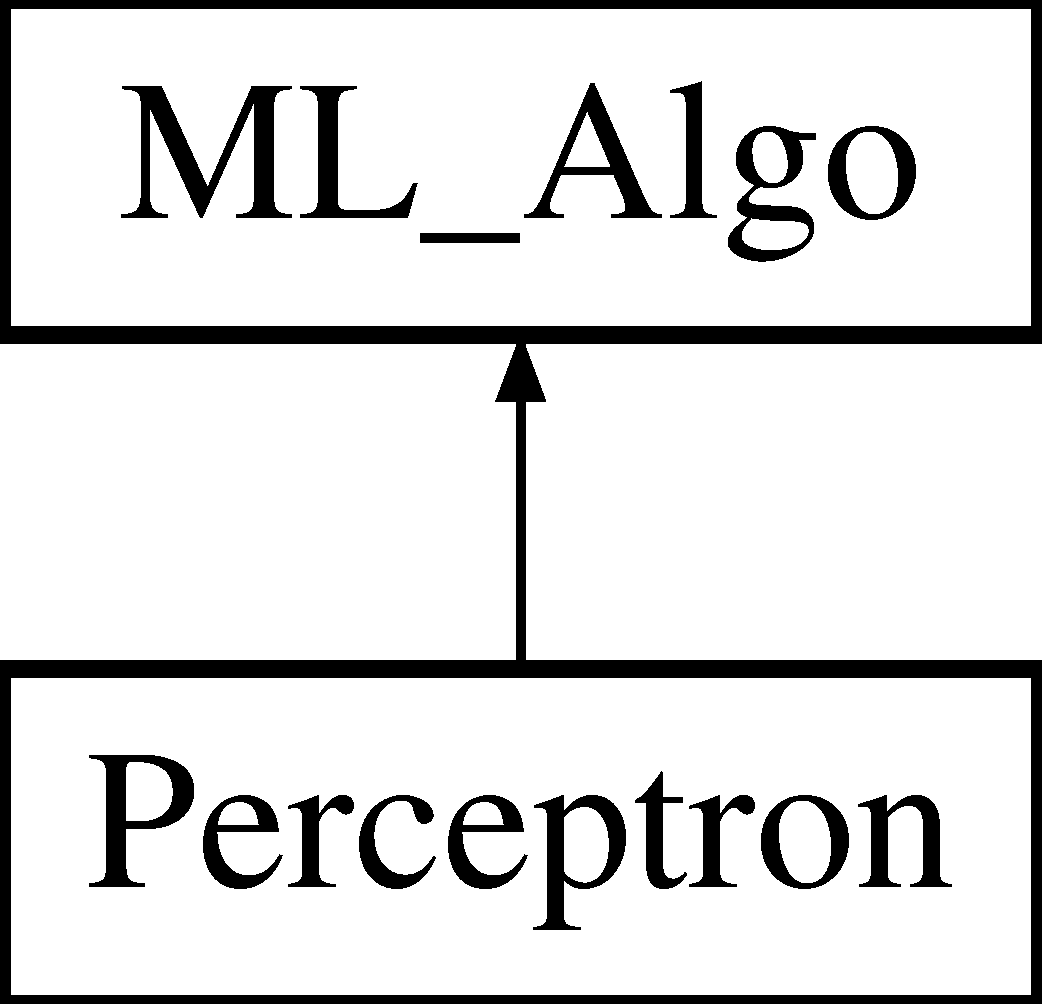
\includegraphics[height=2.000000cm]{classPerceptron}
\end{center}
\end{figure}
\subsection*{Public Member Functions}
\begin{DoxyCompactItemize}
\item 
\hyperlink{classPerceptron_a74b79b672c7d5ac9d69c2f3f66ec09fa}{Perceptron} (void($\ast$f)(const char $\ast$)=N\+U\+LL, int max\+\_\+size=10000)
\item 
virtual \hyperlink{classPerceptron_a0267e40e981df9907129d858911840e7}{$\sim$\+Perceptron} ()
\item 
virtual int \hyperlink{classPerceptron_a2267c5acf9b4a7bd0f47522a530d3863}{prepare\+\_\+training\+\_\+data} (\hyperlink{classStates}{States} $\ast$gsets, int \&pre\+\_\+positive\+\_\+size, int \&pre\+\_\+negative\+\_\+size)
\begin{DoxyCompactList}\small\item\em init training data method. This should be called before any training happens. \end{DoxyCompactList}\item 
virtual int \hyperlink{classPerceptron_adc779991ee63dca333c12fb247b32c9d}{train} ()
\begin{DoxyCompactList}\small\item\em The most important T\+R\+A\+IN method, which calls real training algorithm to do training. \end{DoxyCompactList}\item 
virtual double \hyperlink{classPerceptron_ac9214d2cda4eeb9a06f6562bcb5df8ca}{predict\+\_\+on\+\_\+training\+\_\+set} ()
\begin{DoxyCompactList}\small\item\em Calculate the predict precision of the training-\/model on the training set. \end{DoxyCompactList}\item 
virtual int \hyperlink{classPerceptron_ac7ed76c6a28180691f63f2afbf93cc26}{check\+\_\+question\+\_\+set} (\hyperlink{classStates}{States} \&qset)
\begin{DoxyCompactList}\small\item\em test on question state sets to see if there is an invalidation \end{DoxyCompactList}\item 
virtual int \hyperlink{classPerceptron_a50b1f76eb2760b540477135100dcbf49}{size} ()
\begin{DoxyCompactList}\small\item\em This method returns the current problem size (the number of training states). \end{DoxyCompactList}\item 
virtual \hyperlink{classEquation}{Equation} $\ast$ \hyperlink{classPerceptron_a5408f0ea545d06bbef6630071c73fea2}{roundoff} (int \&num)
\begin{DoxyCompactList}\small\item\em Round off the whole training model.(equations) \end{DoxyCompactList}\item 
virtual int \hyperlink{classPerceptron_a414600a1f189c4f44c858b87048ae655}{predict} (double $\ast$v, int label=0)
\begin{DoxyCompactList}\small\item\em Predict sample x against the whole training model.(equations) \end{DoxyCompactList}\end{DoxyCompactItemize}
\subsection*{Data Fields}
\begin{DoxyCompactItemize}
\item 
\hyperlink{classEquation}{Equation} $\ast$ \hyperlink{classPerceptron_ae021428eb8cf08ebb46383fbc0ea1c46}{main\+\_\+equation}
\item 
double \hyperlink{classPerceptron_a7b395bb8dd492268fc2324c275b8ca4c}{training\+\_\+label} \mbox{[}\hyperlink{config_8h_ab763a0a7202006efe98fe9953784e6a9}{max\+\_\+items} $\ast$2\mbox{]}
\item 
double $\ast$ \hyperlink{classPerceptron_af93816c52b31be423764b53c22733a01}{training\+\_\+set} \mbox{[}\hyperlink{config_8h_ab763a0a7202006efe98fe9953784e6a9}{max\+\_\+items} $\ast$2\mbox{]}
\item 
int \hyperlink{classPerceptron_a996b4296c5e5e4950099a8fe0b37b9df}{length}
\end{DoxyCompactItemize}
\subsection*{Friends}
\begin{DoxyCompactItemize}
\item 
std\+::ostream \& \hyperlink{classPerceptron_a829793c1338f5ab9c9e7e63b6c63be21}{operator$<$$<$} (std\+::ostream \&out, const \hyperlink{classPerceptron}{Perceptron} \&)
\end{DoxyCompactItemize}


\subsection{Constructor \& Destructor Documentation}
\index{Perceptron@{Perceptron}!Perceptron@{Perceptron}}
\index{Perceptron@{Perceptron}!Perceptron@{Perceptron}}
\subsubsection[{Perceptron(void($\ast$f)(const char $\ast$)=\+N\+U\+L\+L, int max\+\_\+size=10000)}]{\setlength{\rightskip}{0pt plus 5cm}Perceptron\+::\+Perceptron (
\begin{DoxyParamCaption}
\item[{void($\ast$)(const char $\ast$)}]{f = {\ttfamily NULL}, }
\item[{int}]{max\+\_\+size = {\ttfamily 10000}}
\end{DoxyParamCaption}
)}\hypertarget{classPerceptron_a74b79b672c7d5ac9d69c2f3f66ec09fa}{}\label{classPerceptron_a74b79b672c7d5ac9d69c2f3f66ec09fa}
\index{Perceptron@{Perceptron}!````~Perceptron@{$\sim$\+Perceptron}}
\index{````~Perceptron@{$\sim$\+Perceptron}!Perceptron@{Perceptron}}
\subsubsection[{$\sim$\+Perceptron()}]{\setlength{\rightskip}{0pt plus 5cm}Perceptron\+::$\sim$\+Perceptron (
\begin{DoxyParamCaption}
{}
\end{DoxyParamCaption}
)\hspace{0.3cm}{\ttfamily [virtual]}}\hypertarget{classPerceptron_a0267e40e981df9907129d858911840e7}{}\label{classPerceptron_a0267e40e981df9907129d858911840e7}


\subsection{Member Function Documentation}
\index{Perceptron@{Perceptron}!check\+\_\+question\+\_\+set@{check\+\_\+question\+\_\+set}}
\index{check\+\_\+question\+\_\+set@{check\+\_\+question\+\_\+set}!Perceptron@{Perceptron}}
\subsubsection[{check\+\_\+question\+\_\+set(\+States \&qset)}]{\setlength{\rightskip}{0pt plus 5cm}int Perceptron\+::check\+\_\+question\+\_\+set (
\begin{DoxyParamCaption}
\item[{{\bf States} \&}]{qset}
\end{DoxyParamCaption}
)\hspace{0.3cm}{\ttfamily [virtual]}}\hypertarget{classPerceptron_ac7ed76c6a28180691f63f2afbf93cc26}{}\label{classPerceptron_ac7ed76c6a28180691f63f2afbf93cc26}


test on question state sets to see if there is an invalidation 

The method will output the inforamtion if a question trace invalidate the training model


\begin{DoxyParams}{Parameters}
{\em qset} & is a reference type to question states. \\
\hline
\end{DoxyParams}
\begin{DoxyReturn}{Returns}
int 0 if no error 
\end{DoxyReturn}


Implements \hyperlink{classML__Algo_a4d757e7fb178ce41ec713bcd84807d33}{M\+L\+\_\+\+Algo}.

\index{Perceptron@{Perceptron}!predict@{predict}}
\index{predict@{predict}!Perceptron@{Perceptron}}
\subsubsection[{predict(double $\ast$v, int label=0)}]{\setlength{\rightskip}{0pt plus 5cm}int Perceptron\+::predict (
\begin{DoxyParamCaption}
\item[{double $\ast$}]{x, }
\item[{int}]{flag = {\ttfamily 0}}
\end{DoxyParamCaption}
)\hspace{0.3cm}{\ttfamily [virtual]}}\hypertarget{classPerceptron_a414600a1f189c4f44c858b87048ae655}{}\label{classPerceptron_a414600a1f189c4f44c858b87048ae655}


Predict sample x against the whole training model.(equations) 


\begin{DoxyParams}{Parameters}
{\em x} & contains the sample to be tested. \\
\hline
{\em flag} & leave this to be Z\+E\+RO... \\
\hline
\end{DoxyParams}
\begin{DoxyReturn}{Returns}
The label of prediction 
\end{DoxyReturn}


Implements \hyperlink{classML__Algo_aae12eabc95fd3eb5305f1ae7a14e0193}{M\+L\+\_\+\+Algo}.

\index{Perceptron@{Perceptron}!predict\+\_\+on\+\_\+training\+\_\+set@{predict\+\_\+on\+\_\+training\+\_\+set}}
\index{predict\+\_\+on\+\_\+training\+\_\+set@{predict\+\_\+on\+\_\+training\+\_\+set}!Perceptron@{Perceptron}}
\subsubsection[{predict\+\_\+on\+\_\+training\+\_\+set()}]{\setlength{\rightskip}{0pt plus 5cm}double Perceptron\+::predict\+\_\+on\+\_\+training\+\_\+set (
\begin{DoxyParamCaption}
{}
\end{DoxyParamCaption}
)\hspace{0.3cm}{\ttfamily [virtual]}}\hypertarget{classPerceptron_ac9214d2cda4eeb9a06f6562bcb5df8ca}{}\label{classPerceptron_ac9214d2cda4eeb9a06f6562bcb5df8ca}


Calculate the predict precision of the training-\/model on the training set. 

\begin{DoxyReturn}{Returns}
double Return precision we can get. Should be a value between 0 and 1. 
\end{DoxyReturn}


Implements \hyperlink{classML__Algo_a39dd640e7c910becf611b9265843ac77}{M\+L\+\_\+\+Algo}.

\index{Perceptron@{Perceptron}!prepare\+\_\+training\+\_\+data@{prepare\+\_\+training\+\_\+data}}
\index{prepare\+\_\+training\+\_\+data@{prepare\+\_\+training\+\_\+data}!Perceptron@{Perceptron}}
\subsubsection[{prepare\+\_\+training\+\_\+data(\+States $\ast$gsets, int \&pre\+\_\+positive\+\_\+size, int \&pre\+\_\+negative\+\_\+size)}]{\setlength{\rightskip}{0pt plus 5cm}int Perceptron\+::prepare\+\_\+training\+\_\+data (
\begin{DoxyParamCaption}
\item[{{\bf States} $\ast$}]{gsets, }
\item[{int \&}]{pre\+\_\+positive\+\_\+size, }
\item[{int \&}]{pre\+\_\+negative\+\_\+size}
\end{DoxyParamCaption}
)\hspace{0.3cm}{\ttfamily [virtual]}}\hypertarget{classPerceptron_a2267c5acf9b4a7bd0f47522a530d3863}{}\label{classPerceptron_a2267c5acf9b4a7bd0f47522a530d3863}


init training data method. This should be called before any training happens. 


\begin{DoxyParams}{Parameters}
{\em gsets} & The states array to store all the generated states information. The size must be 4, and index -\/1 should be accessible \\
\hline
{\em pre\+\_\+positive\+\_\+size} & This records the last positive size of states. And also set by callee to the new value Initially set to 0, as there is no elements in positive states. Calls afterwards should pass the value set by last call. \\
\hline
{\em pre\+\_\+negative\+\_\+size} & This records the last negative size of states. And also set by callee to the new value Initially set to 0, as there is no elements in positive states. Calls afterwards should pass the value set by last call. \\
\hline
\end{DoxyParams}
\begin{DoxyReturn}{Returns}
int 0 if no error 
\end{DoxyReturn}


Implements \hyperlink{classML__Algo_ab98458d234bdf97c2ed678030d90c513}{M\+L\+\_\+\+Algo}.

\index{Perceptron@{Perceptron}!roundoff@{roundoff}}
\index{roundoff@{roundoff}!Perceptron@{Perceptron}}
\subsubsection[{roundoff(int \&num)}]{\setlength{\rightskip}{0pt plus 5cm}{\bf Equation} $\ast$ Perceptron\+::roundoff (
\begin{DoxyParamCaption}
\item[{int \&}]{equation\+\_\+num}
\end{DoxyParamCaption}
)\hspace{0.3cm}{\ttfamily [virtual]}}\hypertarget{classPerceptron_a5408f0ea545d06bbef6630071c73fea2}{}\label{classPerceptron_a5408f0ea545d06bbef6630071c73fea2}


Round off the whole training model.(equations) 


\begin{DoxyParams}{Parameters}
{\em equation\+\_\+num} & set by callee to notify the number of equations we currently get \\
\hline
\end{DoxyParams}
\begin{DoxyReturn}{Returns}
Eqation Point the rounded off equations. Remember to D\+E\+L\+E\+TE them after use by caller. Otherwise memory leak. 
\end{DoxyReturn}


Implements \hyperlink{classML__Algo_a398214e0462ebfdde10e745240030a34}{M\+L\+\_\+\+Algo}.

\index{Perceptron@{Perceptron}!size@{size}}
\index{size@{size}!Perceptron@{Perceptron}}
\subsubsection[{size()}]{\setlength{\rightskip}{0pt plus 5cm}int Perceptron\+::size (
\begin{DoxyParamCaption}
{}
\end{DoxyParamCaption}
)\hspace{0.3cm}{\ttfamily [virtual]}}\hypertarget{classPerceptron_a50b1f76eb2760b540477135100dcbf49}{}\label{classPerceptron_a50b1f76eb2760b540477135100dcbf49}


This method returns the current problem size (the number of training states). 

\begin{DoxyReturn}{Returns}
int the size of problem 
\end{DoxyReturn}


Implements \hyperlink{classML__Algo_a8650c3894c1992492f8bc86edf1b3ffd}{M\+L\+\_\+\+Algo}.

\index{Perceptron@{Perceptron}!train@{train}}
\index{train@{train}!Perceptron@{Perceptron}}
\subsubsection[{train()}]{\setlength{\rightskip}{0pt plus 5cm}int Perceptron\+::train (
\begin{DoxyParamCaption}
{}
\end{DoxyParamCaption}
)\hspace{0.3cm}{\ttfamily [virtual]}}\hypertarget{classPerceptron_adc779991ee63dca333c12fb247b32c9d}{}\label{classPerceptron_adc779991ee63dca333c12fb247b32c9d}


The most important T\+R\+A\+IN method, which calls real training algorithm to do training. 

\begin{DoxyReturn}{Returns}
int 0 if no error. 
\end{DoxyReturn}


Implements \hyperlink{classML__Algo_a0a5d241191d4249c60a40d966fb19aee}{M\+L\+\_\+\+Algo}.



\subsection{Friends And Related Function Documentation}
\index{Perceptron@{Perceptron}!operator$<$$<$@{operator$<$$<$}}
\index{operator$<$$<$@{operator$<$$<$}!Perceptron@{Perceptron}}
\subsubsection[{operator$<$$<$}]{\setlength{\rightskip}{0pt plus 5cm}std\+::ostream\& operator$<$$<$ (
\begin{DoxyParamCaption}
\item[{std\+::ostream \&}]{out, }
\item[{const {\bf Perceptron} \&}]{perceptron}
\end{DoxyParamCaption}
)\hspace{0.3cm}{\ttfamily [friend]}}\hypertarget{classPerceptron_a829793c1338f5ab9c9e7e63b6c63be21}{}\label{classPerceptron_a829793c1338f5ab9c9e7e63b6c63be21}


\subsection{Field Documentation}
\index{Perceptron@{Perceptron}!length@{length}}
\index{length@{length}!Perceptron@{Perceptron}}
\subsubsection[{length}]{\setlength{\rightskip}{0pt plus 5cm}int Perceptron\+::length}\hypertarget{classPerceptron_a996b4296c5e5e4950099a8fe0b37b9df}{}\label{classPerceptron_a996b4296c5e5e4950099a8fe0b37b9df}
\index{Perceptron@{Perceptron}!main\+\_\+equation@{main\+\_\+equation}}
\index{main\+\_\+equation@{main\+\_\+equation}!Perceptron@{Perceptron}}
\subsubsection[{main\+\_\+equation}]{\setlength{\rightskip}{0pt plus 5cm}{\bf Equation}$\ast$ Perceptron\+::main\+\_\+equation}\hypertarget{classPerceptron_ae021428eb8cf08ebb46383fbc0ea1c46}{}\label{classPerceptron_ae021428eb8cf08ebb46383fbc0ea1c46}
\index{Perceptron@{Perceptron}!training\+\_\+label@{training\+\_\+label}}
\index{training\+\_\+label@{training\+\_\+label}!Perceptron@{Perceptron}}
\subsubsection[{training\+\_\+label}]{\setlength{\rightskip}{0pt plus 5cm}double Perceptron\+::training\+\_\+label\mbox{[}{\bf max\+\_\+items} $\ast$2\mbox{]}}\hypertarget{classPerceptron_a7b395bb8dd492268fc2324c275b8ca4c}{}\label{classPerceptron_a7b395bb8dd492268fc2324c275b8ca4c}
\index{Perceptron@{Perceptron}!training\+\_\+set@{training\+\_\+set}}
\index{training\+\_\+set@{training\+\_\+set}!Perceptron@{Perceptron}}
\subsubsection[{training\+\_\+set}]{\setlength{\rightskip}{0pt plus 5cm}double$\ast$ Perceptron\+::training\+\_\+set\mbox{[}{\bf max\+\_\+items} $\ast$2\mbox{]}}\hypertarget{classPerceptron_af93816c52b31be423764b53c22733a01}{}\label{classPerceptron_af93816c52b31be423764b53c22733a01}


The documentation for this class was generated from the following files\+:\begin{DoxyCompactItemize}
\item 
include/\hyperlink{perceptron_8h}{perceptron.\+h}\item 
src/\hyperlink{perceptron_8cpp}{perceptron.\+cpp}\end{DoxyCompactItemize}

\hypertarget{classQMatrix}{}\section{Q\+Matrix Class Reference}
\label{classQMatrix}\index{Q\+Matrix@{Q\+Matrix}}
Inheritance diagram for Q\+Matrix\+:\begin{figure}[H]
\begin{center}
\leavevmode
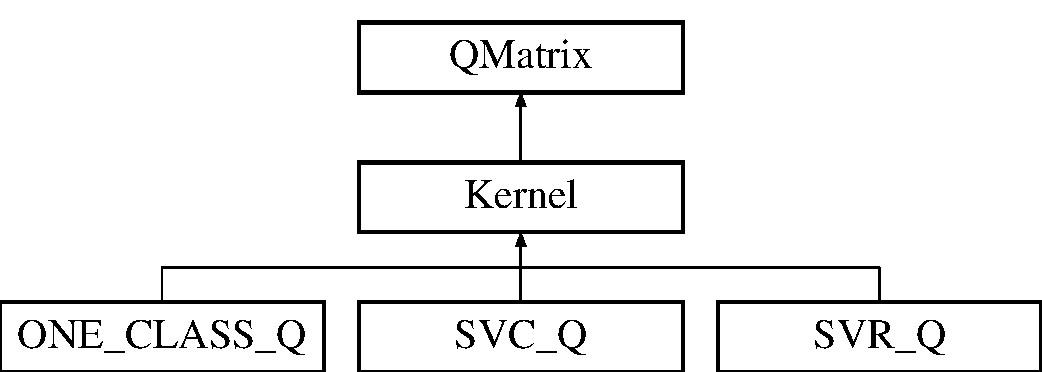
\includegraphics[height=3.000000cm]{classQMatrix}
\end{center}
\end{figure}
\subsection*{Public Member Functions}
\begin{DoxyCompactItemize}
\item 
virtual \hyperlink{svm__core_8cpp_a8755d90a54ecfb8d15051af3e0542592}{Qfloat} $\ast$ \hyperlink{classQMatrix_aba360e5c50764e2dd013555d20c861f5}{get\+\_\+Q} (int column, int len) const  =0
\item 
virtual double $\ast$ \hyperlink{classQMatrix_a8fa3bebbb30838d2eef68afdb6da1024}{get\+\_\+\+QD} () const  =0
\item 
virtual void \hyperlink{classQMatrix_a095e38cbf4a02cfb1acc2377f8370628}{swap\+\_\+index} (int i, int j) const  =0
\item 
virtual \hyperlink{classQMatrix_a52846254a40a7fa23fa31515ceb99ce1}{$\sim$\+Q\+Matrix} ()
\end{DoxyCompactItemize}


\subsection{Constructor \& Destructor Documentation}
\index{Q\+Matrix@{Q\+Matrix}!````~Q\+Matrix@{$\sim$\+Q\+Matrix}}
\index{````~Q\+Matrix@{$\sim$\+Q\+Matrix}!Q\+Matrix@{Q\+Matrix}}
\subsubsection[{$\sim$\+Q\+Matrix()}]{\setlength{\rightskip}{0pt plus 5cm}virtual Q\+Matrix\+::$\sim$\+Q\+Matrix (
\begin{DoxyParamCaption}
{}
\end{DoxyParamCaption}
)\hspace{0.3cm}{\ttfamily [inline]}, {\ttfamily [virtual]}}\hypertarget{classQMatrix_a52846254a40a7fa23fa31515ceb99ce1}{}\label{classQMatrix_a52846254a40a7fa23fa31515ceb99ce1}


\subsection{Member Function Documentation}
\index{Q\+Matrix@{Q\+Matrix}!get\+\_\+Q@{get\+\_\+Q}}
\index{get\+\_\+Q@{get\+\_\+Q}!Q\+Matrix@{Q\+Matrix}}
\subsubsection[{get\+\_\+\+Q(int column, int len) const  =0}]{\setlength{\rightskip}{0pt plus 5cm}virtual {\bf Qfloat}$\ast$ Q\+Matrix\+::get\+\_\+Q (
\begin{DoxyParamCaption}
\item[{int}]{column, }
\item[{int}]{len}
\end{DoxyParamCaption}
) const\hspace{0.3cm}{\ttfamily [pure virtual]}}\hypertarget{classQMatrix_aba360e5c50764e2dd013555d20c861f5}{}\label{classQMatrix_aba360e5c50764e2dd013555d20c861f5}


Implemented in \hyperlink{classSVR__Q_aba55078d17e7815f093ffa154f3cee9d}{S\+V\+R\+\_\+Q}, \hyperlink{classONE__CLASS__Q_a1f8501234022e017cf46c4dfb2da9d31}{O\+N\+E\+\_\+\+C\+L\+A\+S\+S\+\_\+Q}, \hyperlink{classSVC__Q_a9341b6030b3fdc88466e4a602b5abff0}{S\+V\+C\+\_\+Q}, and \hyperlink{classKernel_a02f328649424359b92b941f5219a6060}{Kernel}.

\index{Q\+Matrix@{Q\+Matrix}!get\+\_\+\+QD@{get\+\_\+\+QD}}
\index{get\+\_\+\+QD@{get\+\_\+\+QD}!Q\+Matrix@{Q\+Matrix}}
\subsubsection[{get\+\_\+\+Q\+D() const  =0}]{\setlength{\rightskip}{0pt plus 5cm}virtual double$\ast$ Q\+Matrix\+::get\+\_\+\+QD (
\begin{DoxyParamCaption}
{}
\end{DoxyParamCaption}
) const\hspace{0.3cm}{\ttfamily [pure virtual]}}\hypertarget{classQMatrix_a8fa3bebbb30838d2eef68afdb6da1024}{}\label{classQMatrix_a8fa3bebbb30838d2eef68afdb6da1024}


Implemented in \hyperlink{classSVR__Q_ac22ed5ce1b0bf6a900c3c8d631e77d76}{S\+V\+R\+\_\+Q}, \hyperlink{classONE__CLASS__Q_a882480d4370d8a89d667a28c3ed68a73}{O\+N\+E\+\_\+\+C\+L\+A\+S\+S\+\_\+Q}, \hyperlink{classSVC__Q_ac73020a6e438e209d63223e1fa8cac29}{S\+V\+C\+\_\+Q}, and \hyperlink{classKernel_a7bf9602583da1af48d15d19da69514ac}{Kernel}.

\index{Q\+Matrix@{Q\+Matrix}!swap\+\_\+index@{swap\+\_\+index}}
\index{swap\+\_\+index@{swap\+\_\+index}!Q\+Matrix@{Q\+Matrix}}
\subsubsection[{swap\+\_\+index(int i, int j) const  =0}]{\setlength{\rightskip}{0pt plus 5cm}virtual void Q\+Matrix\+::swap\+\_\+index (
\begin{DoxyParamCaption}
\item[{int}]{i, }
\item[{int}]{j}
\end{DoxyParamCaption}
) const\hspace{0.3cm}{\ttfamily [pure virtual]}}\hypertarget{classQMatrix_a095e38cbf4a02cfb1acc2377f8370628}{}\label{classQMatrix_a095e38cbf4a02cfb1acc2377f8370628}


Implemented in \hyperlink{classSVR__Q_a9d3884f0c68f4ce18d47570e4a203405}{S\+V\+R\+\_\+Q}, \hyperlink{classONE__CLASS__Q_ad8bc86ca742c27d82718346388f83fad}{O\+N\+E\+\_\+\+C\+L\+A\+S\+S\+\_\+Q}, \hyperlink{classSVC__Q_a9c889db8ee0156ed5bcdaa4d6bc4e245}{S\+V\+C\+\_\+Q}, and \hyperlink{classKernel_adca807c5584bc42fd098cd9eb1f19621}{Kernel}.



The documentation for this class was generated from the following file\+:\begin{DoxyCompactItemize}
\item 
src/\hyperlink{svm__core_8cpp}{svm\+\_\+core.\+cpp}\end{DoxyCompactItemize}

\hypertarget{classSolution}{}\section{Solution Class Reference}
\label{classSolution}\index{Solution@{Solution}}


This class defines the format of a valid solution to an equation.  




{\ttfamily \#include $<$equation.\+h$>$}

\subsection*{Public Member Functions}
\begin{DoxyCompactItemize}
\item 
\hyperlink{classSolution_ab55bd4b023d596ce11aaf737b9a6123b}{Solution} ()
\begin{DoxyCompactList}\small\item\em Default constructor. Set all its elements to value 0. \end{DoxyCompactList}\item 
\hyperlink{classSolution_a2b382bc23a6b180f2ed161707da039dd}{Solution} (double a0,...)
\begin{DoxyCompactList}\small\item\em Most useful constructor Set its elements to the given values, order keeps. \end{DoxyCompactList}\end{DoxyCompactItemize}
\subsection*{Data Fields}
\begin{DoxyCompactItemize}
\item 
double \hyperlink{classSolution_a67672e91e753de458afef2ca270510dd}{x} \mbox{[}\hyperlink{config_8h_a1d6565a8ececd15de44965eec4790919}{V\+A\+RS}\mbox{]}
\begin{DoxyCompactList}\small\item\em The data field of \hyperlink{classSolution}{Solution}, stores all the values as a solution to an \hyperlink{classEquation}{Equation}. \end{DoxyCompactList}\end{DoxyCompactItemize}
\subsection*{Friends}
\begin{DoxyCompactItemize}
\item 
std\+::ostream \& \hyperlink{classSolution_a57557999df406fb734b29cff24838d80}{operator$<$$<$} (std\+::ostream \&out, const \hyperlink{classSolution}{Solution} \&sol)
\begin{DoxyCompactList}\small\item\em support $<$$<$ operator simply output its elements as a tuple \end{DoxyCompactList}\end{DoxyCompactItemize}


\subsection{Detailed Description}
This class defines the format of a valid solution to an equation. 

It contains values to each variants in an equation 

\subsection{Constructor \& Destructor Documentation}
\index{Solution@{Solution}!Solution@{Solution}}
\index{Solution@{Solution}!Solution@{Solution}}
\subsubsection[{Solution()}]{\setlength{\rightskip}{0pt plus 5cm}Solution\+::\+Solution (
\begin{DoxyParamCaption}
{}
\end{DoxyParamCaption}
)}\hypertarget{classSolution_ab55bd4b023d596ce11aaf737b9a6123b}{}\label{classSolution_ab55bd4b023d596ce11aaf737b9a6123b}


Default constructor. Set all its elements to value 0. 

\index{Solution@{Solution}!Solution@{Solution}}
\index{Solution@{Solution}!Solution@{Solution}}
\subsubsection[{Solution(double a0,...)}]{\setlength{\rightskip}{0pt plus 5cm}Solution\+::\+Solution (
\begin{DoxyParamCaption}
\item[{double}]{a0, }
\item[{}]{...}
\end{DoxyParamCaption}
)}\hypertarget{classSolution_a2b382bc23a6b180f2ed161707da039dd}{}\label{classSolution_a2b382bc23a6b180f2ed161707da039dd}


Most useful constructor Set its elements to the given values, order keeps. 


\begin{DoxyParams}{Parameters}
{\em a0...} & each element values for a solution \\
\hline
\end{DoxyParams}


\subsection{Friends And Related Function Documentation}
\index{Solution@{Solution}!operator$<$$<$@{operator$<$$<$}}
\index{operator$<$$<$@{operator$<$$<$}!Solution@{Solution}}
\subsubsection[{operator$<$$<$}]{\setlength{\rightskip}{0pt plus 5cm}std\+::ostream\& operator$<$$<$ (
\begin{DoxyParamCaption}
\item[{std\+::ostream \&}]{out, }
\item[{const {\bf Solution} \&}]{sol}
\end{DoxyParamCaption}
)\hspace{0.3cm}{\ttfamily [friend]}}\hypertarget{classSolution_a57557999df406fb734b29cff24838d80}{}\label{classSolution_a57557999df406fb734b29cff24838d80}


support $<$$<$ operator simply output its elements as a tuple 


\begin{DoxyParams}{Parameters}
{\em sol} & The solution object to be output \\
\hline
\end{DoxyParams}


\subsection{Field Documentation}
\index{Solution@{Solution}!x@{x}}
\index{x@{x}!Solution@{Solution}}
\subsubsection[{x}]{\setlength{\rightskip}{0pt plus 5cm}double Solution\+::x\mbox{[}{\bf V\+A\+RS}\mbox{]}}\hypertarget{classSolution_a67672e91e753de458afef2ca270510dd}{}\label{classSolution_a67672e91e753de458afef2ca270510dd}


The data field of \hyperlink{classSolution}{Solution}, stores all the values as a solution to an \hyperlink{classEquation}{Equation}. 



The documentation for this class was generated from the following files\+:\begin{DoxyCompactItemize}
\item 
include/\hyperlink{equation_8h}{equation.\+h}\item 
src/\hyperlink{equation_8cpp}{equation.\+cpp}\end{DoxyCompactItemize}

\hypertarget{structSolver_1_1SolutionInfo}{}\section{Solver\+:\+:Solution\+Info Struct Reference}
\label{structSolver_1_1SolutionInfo}\index{Solver\+::\+Solution\+Info@{Solver\+::\+Solution\+Info}}
\subsection*{Data Fields}
\begin{DoxyCompactItemize}
\item 
double \hyperlink{structSolver_1_1SolutionInfo_adf1d775e9152a7b1742057cd638ed2ae}{obj}
\item 
double \hyperlink{structSolver_1_1SolutionInfo_a8091f45a336af39e232f3845e25f2266}{rho}
\item 
double \hyperlink{structSolver_1_1SolutionInfo_a94c4cb7f402752326cc975ec57a8688f}{upper\+\_\+bound\+\_\+p}
\item 
double \hyperlink{structSolver_1_1SolutionInfo_a07ab9dc3265855f483922988bdaaf986}{upper\+\_\+bound\+\_\+n}
\item 
double \hyperlink{structSolver_1_1SolutionInfo_a3db948f9e914e1f9976523cfdc7c1bbe}{r}
\end{DoxyCompactItemize}


\subsection{Field Documentation}
\index{Solver\+::\+Solution\+Info@{Solver\+::\+Solution\+Info}!obj@{obj}}
\index{obj@{obj}!Solver\+::\+Solution\+Info@{Solver\+::\+Solution\+Info}}
\subsubsection[{obj}]{\setlength{\rightskip}{0pt plus 5cm}double Solver\+::\+Solution\+Info\+::obj}\hypertarget{structSolver_1_1SolutionInfo_adf1d775e9152a7b1742057cd638ed2ae}{}\label{structSolver_1_1SolutionInfo_adf1d775e9152a7b1742057cd638ed2ae}
\index{Solver\+::\+Solution\+Info@{Solver\+::\+Solution\+Info}!r@{r}}
\index{r@{r}!Solver\+::\+Solution\+Info@{Solver\+::\+Solution\+Info}}
\subsubsection[{r}]{\setlength{\rightskip}{0pt plus 5cm}double Solver\+::\+Solution\+Info\+::r}\hypertarget{structSolver_1_1SolutionInfo_a3db948f9e914e1f9976523cfdc7c1bbe}{}\label{structSolver_1_1SolutionInfo_a3db948f9e914e1f9976523cfdc7c1bbe}
\index{Solver\+::\+Solution\+Info@{Solver\+::\+Solution\+Info}!rho@{rho}}
\index{rho@{rho}!Solver\+::\+Solution\+Info@{Solver\+::\+Solution\+Info}}
\subsubsection[{rho}]{\setlength{\rightskip}{0pt plus 5cm}double Solver\+::\+Solution\+Info\+::rho}\hypertarget{structSolver_1_1SolutionInfo_a8091f45a336af39e232f3845e25f2266}{}\label{structSolver_1_1SolutionInfo_a8091f45a336af39e232f3845e25f2266}
\index{Solver\+::\+Solution\+Info@{Solver\+::\+Solution\+Info}!upper\+\_\+bound\+\_\+n@{upper\+\_\+bound\+\_\+n}}
\index{upper\+\_\+bound\+\_\+n@{upper\+\_\+bound\+\_\+n}!Solver\+::\+Solution\+Info@{Solver\+::\+Solution\+Info}}
\subsubsection[{upper\+\_\+bound\+\_\+n}]{\setlength{\rightskip}{0pt plus 5cm}double Solver\+::\+Solution\+Info\+::upper\+\_\+bound\+\_\+n}\hypertarget{structSolver_1_1SolutionInfo_a07ab9dc3265855f483922988bdaaf986}{}\label{structSolver_1_1SolutionInfo_a07ab9dc3265855f483922988bdaaf986}
\index{Solver\+::\+Solution\+Info@{Solver\+::\+Solution\+Info}!upper\+\_\+bound\+\_\+p@{upper\+\_\+bound\+\_\+p}}
\index{upper\+\_\+bound\+\_\+p@{upper\+\_\+bound\+\_\+p}!Solver\+::\+Solution\+Info@{Solver\+::\+Solution\+Info}}
\subsubsection[{upper\+\_\+bound\+\_\+p}]{\setlength{\rightskip}{0pt plus 5cm}double Solver\+::\+Solution\+Info\+::upper\+\_\+bound\+\_\+p}\hypertarget{structSolver_1_1SolutionInfo_a94c4cb7f402752326cc975ec57a8688f}{}\label{structSolver_1_1SolutionInfo_a94c4cb7f402752326cc975ec57a8688f}


The documentation for this struct was generated from the following file\+:\begin{DoxyCompactItemize}
\item 
src/\hyperlink{svm__core_8cpp}{svm\+\_\+core.\+cpp}\end{DoxyCompactItemize}

\hypertarget{classSolver}{}\section{Solver Class Reference}
\label{classSolver}\index{Solver@{Solver}}
Inheritance diagram for Solver\+:\begin{figure}[H]
\begin{center}
\leavevmode
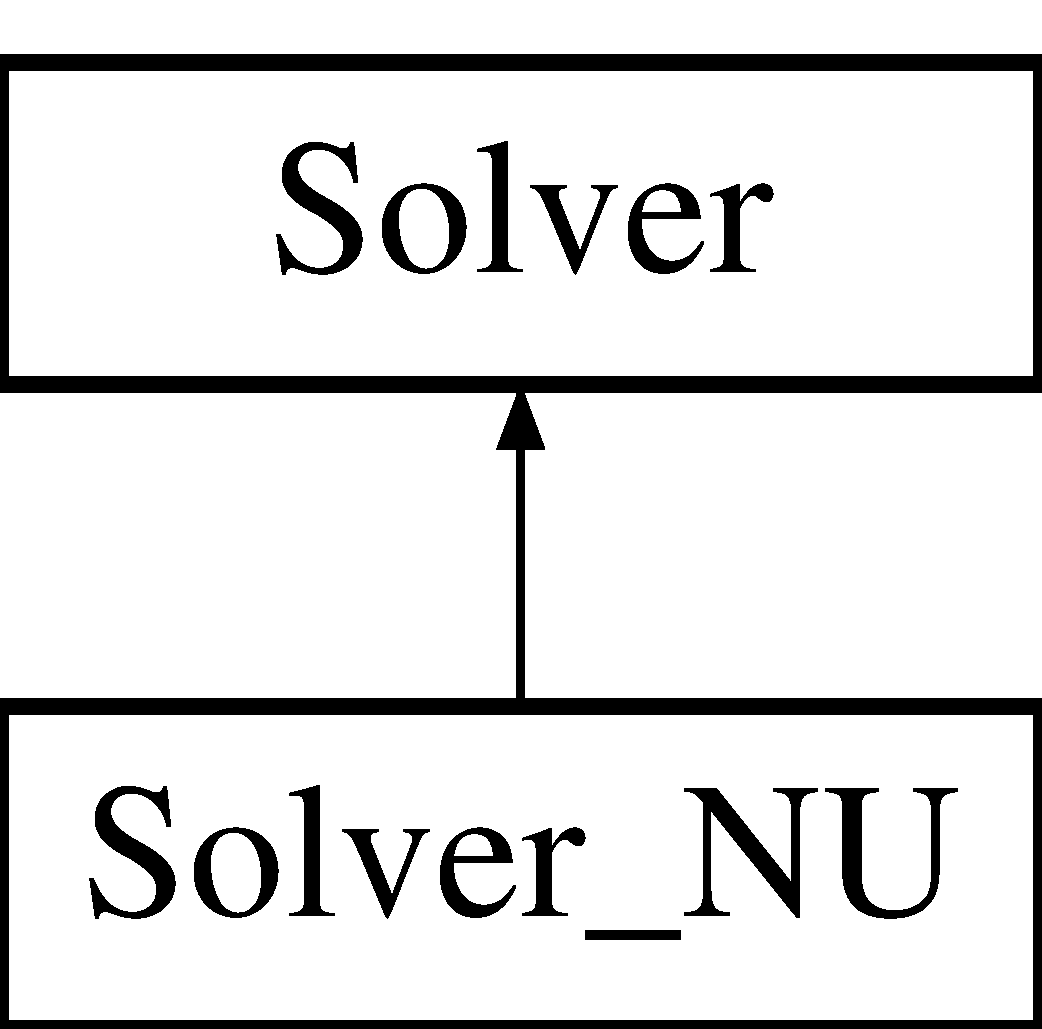
\includegraphics[height=2.000000cm]{classSolver}
\end{center}
\end{figure}
\subsection*{Data Structures}
\begin{DoxyCompactItemize}
\item 
struct \hyperlink{structSolver_1_1SolutionInfo}{Solution\+Info}
\end{DoxyCompactItemize}
\subsection*{Public Member Functions}
\begin{DoxyCompactItemize}
\item 
\hyperlink{classSolver_a9dfe7ae9ce617e8a6398be34284c907a}{Solver} ()
\item 
virtual \hyperlink{classSolver_a14f7014dd6e46e3990dea30b5ad3c087}{$\sim$\+Solver} ()
\item 
void \hyperlink{classSolver_aa3ab5672a26826f9dc1ac9145620a823}{Solve} (int \hyperlink{classSolver_a88832d45b6de977b1cbb2afd4c0e494c}{l}, const \hyperlink{classQMatrix}{Q\+Matrix} \&\hyperlink{classSolver_a2d3461718f0570bdc47f5dfb31d61e0a}{Q}, const double $\ast$p\+\_\+, const \hyperlink{svm__core_8cpp_a0fd9ce9d735064461bebfe6037026093}{schar} $\ast$y\+\_\+, double $\ast$alpha\+\_\+, double \hyperlink{classSolver_a2e45dbea8be469bf8247e14768549dd5}{Cp}, double \hyperlink{classSolver_a38d741d194839fb445f982dd78e0b97b}{Cn}, double \hyperlink{classSolver_a718333cc2c1d40abf9c292a788cba1e5}{eps}, \hyperlink{structSolver_1_1SolutionInfo}{Solution\+Info} $\ast$si, int shrinking)
\end{DoxyCompactItemize}
\subsection*{Protected Types}
\begin{DoxyCompactItemize}
\item 
enum \{ \hyperlink{classSolver_a86c1a7637bc803ef8496c7dbf7f00b03aeb78558e05ec0672378c3e801e866560}{L\+O\+W\+E\+R\+\_\+\+B\+O\+U\+ND}, 
\hyperlink{classSolver_a86c1a7637bc803ef8496c7dbf7f00b03aef825a32b2471cdb0724cfa9c1f051fd}{U\+P\+P\+E\+R\+\_\+\+B\+O\+U\+ND}, 
\hyperlink{classSolver_a86c1a7637bc803ef8496c7dbf7f00b03a904f6af2170b6f900fbd3d46cd055c76}{F\+R\+EE}
 \}
\end{DoxyCompactItemize}
\subsection*{Protected Member Functions}
\begin{DoxyCompactItemize}
\item 
double \hyperlink{classSolver_ae55a8581815436d13e760dadaec34e2a}{get\+\_\+C} (int i)
\item 
void \hyperlink{classSolver_a5a978b4ff9b60b2d75e54970fd6a2c20}{update\+\_\+alpha\+\_\+status} (int i)
\item 
bool \hyperlink{classSolver_a98d878b13d6f710fcaa0b16e657a37b6}{is\+\_\+upper\+\_\+bound} (int i)
\item 
bool \hyperlink{classSolver_a5876eedb0a6de6954f6037af0992cbed}{is\+\_\+lower\+\_\+bound} (int i)
\item 
bool \hyperlink{classSolver_a7b5e230875b8b5f06150ff0690e36b47}{is\+\_\+free} (int i)
\item 
void \hyperlink{classSolver_a043f498c1dda0122859d03f9cd07dc08}{swap\+\_\+index} (int i, int j)
\item 
void \hyperlink{classSolver_a7e34992ede606a336606ae54f6e963e6}{reconstruct\+\_\+gradient} ()
\item 
virtual int \hyperlink{classSolver_a95fb4eaf33362558e1fc768f4db019d3}{select\+\_\+working\+\_\+set} (int \&i, int \&j)
\item 
virtual double \hyperlink{classSolver_ad00b01f72232ca932cad68e58c9cde5a}{calculate\+\_\+rho} ()
\item 
virtual void \hyperlink{classSolver_ad3f6665a1ca590e56b3d51f8ddcc347c}{do\+\_\+shrinking} ()
\end{DoxyCompactItemize}
\subsection*{Protected Attributes}
\begin{DoxyCompactItemize}
\item 
int \hyperlink{classSolver_a06ba1b87b3749cc545e573151b7beca0}{active\+\_\+size}
\item 
\hyperlink{svm__core_8cpp_a0fd9ce9d735064461bebfe6037026093}{schar} $\ast$ \hyperlink{classSolver_a3acc1043d06dedf87f054ff3eea5c426}{y}
\item 
double $\ast$ \hyperlink{classSolver_ad8ab27068f2e045591970aae1201afe9}{G}
\item 
char $\ast$ \hyperlink{classSolver_a9fe653e04c43956d5fb86635651b0003}{alpha\+\_\+status}
\item 
double $\ast$ \hyperlink{classSolver_a00d7a7cefa2504d41c7db6cd7cc6b428}{alpha}
\item 
const \hyperlink{classQMatrix}{Q\+Matrix} $\ast$ \hyperlink{classSolver_a2d3461718f0570bdc47f5dfb31d61e0a}{Q}
\item 
const double $\ast$ \hyperlink{classSolver_a7c7b7b1207983543855165e8eb249f2a}{QD}
\item 
double \hyperlink{classSolver_a718333cc2c1d40abf9c292a788cba1e5}{eps}
\item 
double \hyperlink{classSolver_a2e45dbea8be469bf8247e14768549dd5}{Cp}
\item 
double \hyperlink{classSolver_a38d741d194839fb445f982dd78e0b97b}{Cn}
\item 
double $\ast$ \hyperlink{classSolver_a882cce072f56679880d409e3e73f7ae8}{p}
\item 
int $\ast$ \hyperlink{classSolver_a6382277606a9b3df3d2f0ac947e1cde3}{active\+\_\+set}
\item 
double $\ast$ \hyperlink{classSolver_a89e58cf39a0415c9032b8ec2f4575dcc}{G\+\_\+bar}
\item 
int \hyperlink{classSolver_a88832d45b6de977b1cbb2afd4c0e494c}{l}
\item 
bool \hyperlink{classSolver_a62ded1c184aeb28f8dee04eb4a10530a}{unshrink}
\end{DoxyCompactItemize}


\subsection{Member Enumeration Documentation}
\subsubsection[{anonymous enum}]{\setlength{\rightskip}{0pt plus 5cm}anonymous enum\hspace{0.3cm}{\ttfamily [protected]}}\hypertarget{classSolver_a86c1a7637bc803ef8496c7dbf7f00b03}{}\label{classSolver_a86c1a7637bc803ef8496c7dbf7f00b03}
\begin{Desc}
\item[Enumerator]\par
\begin{description}
\index{L\+O\+W\+E\+R\+\_\+\+B\+O\+U\+ND@{L\+O\+W\+E\+R\+\_\+\+B\+O\+U\+ND}!Solver@{Solver}}\index{Solver@{Solver}!L\+O\+W\+E\+R\+\_\+\+B\+O\+U\+ND@{L\+O\+W\+E\+R\+\_\+\+B\+O\+U\+ND}}\item[{\em 
L\+O\+W\+E\+R\+\_\+\+B\+O\+U\+ND\hypertarget{classSolver_a86c1a7637bc803ef8496c7dbf7f00b03aeb78558e05ec0672378c3e801e866560}{}\label{classSolver_a86c1a7637bc803ef8496c7dbf7f00b03aeb78558e05ec0672378c3e801e866560}
}]\index{U\+P\+P\+E\+R\+\_\+\+B\+O\+U\+ND@{U\+P\+P\+E\+R\+\_\+\+B\+O\+U\+ND}!Solver@{Solver}}\index{Solver@{Solver}!U\+P\+P\+E\+R\+\_\+\+B\+O\+U\+ND@{U\+P\+P\+E\+R\+\_\+\+B\+O\+U\+ND}}\item[{\em 
U\+P\+P\+E\+R\+\_\+\+B\+O\+U\+ND\hypertarget{classSolver_a86c1a7637bc803ef8496c7dbf7f00b03aef825a32b2471cdb0724cfa9c1f051fd}{}\label{classSolver_a86c1a7637bc803ef8496c7dbf7f00b03aef825a32b2471cdb0724cfa9c1f051fd}
}]\index{F\+R\+EE@{F\+R\+EE}!Solver@{Solver}}\index{Solver@{Solver}!F\+R\+EE@{F\+R\+EE}}\item[{\em 
F\+R\+EE\hypertarget{classSolver_a86c1a7637bc803ef8496c7dbf7f00b03a904f6af2170b6f900fbd3d46cd055c76}{}\label{classSolver_a86c1a7637bc803ef8496c7dbf7f00b03a904f6af2170b6f900fbd3d46cd055c76}
}]\end{description}
\end{Desc}


\subsection{Constructor \& Destructor Documentation}
\index{Solver@{Solver}!Solver@{Solver}}
\index{Solver@{Solver}!Solver@{Solver}}
\subsubsection[{Solver()}]{\setlength{\rightskip}{0pt plus 5cm}Solver\+::\+Solver (
\begin{DoxyParamCaption}
{}
\end{DoxyParamCaption}
)\hspace{0.3cm}{\ttfamily [inline]}}\hypertarget{classSolver_a9dfe7ae9ce617e8a6398be34284c907a}{}\label{classSolver_a9dfe7ae9ce617e8a6398be34284c907a}
\index{Solver@{Solver}!````~Solver@{$\sim$\+Solver}}
\index{````~Solver@{$\sim$\+Solver}!Solver@{Solver}}
\subsubsection[{$\sim$\+Solver()}]{\setlength{\rightskip}{0pt plus 5cm}virtual Solver\+::$\sim$\+Solver (
\begin{DoxyParamCaption}
{}
\end{DoxyParamCaption}
)\hspace{0.3cm}{\ttfamily [inline]}, {\ttfamily [virtual]}}\hypertarget{classSolver_a14f7014dd6e46e3990dea30b5ad3c087}{}\label{classSolver_a14f7014dd6e46e3990dea30b5ad3c087}


\subsection{Member Function Documentation}
\index{Solver@{Solver}!calculate\+\_\+rho@{calculate\+\_\+rho}}
\index{calculate\+\_\+rho@{calculate\+\_\+rho}!Solver@{Solver}}
\subsubsection[{calculate\+\_\+rho()}]{\setlength{\rightskip}{0pt plus 5cm}double Solver\+::calculate\+\_\+rho (
\begin{DoxyParamCaption}
{}
\end{DoxyParamCaption}
)\hspace{0.3cm}{\ttfamily [protected]}, {\ttfamily [virtual]}}\hypertarget{classSolver_ad00b01f72232ca932cad68e58c9cde5a}{}\label{classSolver_ad00b01f72232ca932cad68e58c9cde5a}
\index{Solver@{Solver}!do\+\_\+shrinking@{do\+\_\+shrinking}}
\index{do\+\_\+shrinking@{do\+\_\+shrinking}!Solver@{Solver}}
\subsubsection[{do\+\_\+shrinking()}]{\setlength{\rightskip}{0pt plus 5cm}void Solver\+::do\+\_\+shrinking (
\begin{DoxyParamCaption}
{}
\end{DoxyParamCaption}
)\hspace{0.3cm}{\ttfamily [protected]}, {\ttfamily [virtual]}}\hypertarget{classSolver_ad3f6665a1ca590e56b3d51f8ddcc347c}{}\label{classSolver_ad3f6665a1ca590e56b3d51f8ddcc347c}
\index{Solver@{Solver}!get\+\_\+C@{get\+\_\+C}}
\index{get\+\_\+C@{get\+\_\+C}!Solver@{Solver}}
\subsubsection[{get\+\_\+\+C(int i)}]{\setlength{\rightskip}{0pt plus 5cm}double Solver\+::get\+\_\+C (
\begin{DoxyParamCaption}
\item[{int}]{i}
\end{DoxyParamCaption}
)\hspace{0.3cm}{\ttfamily [inline]}, {\ttfamily [protected]}}\hypertarget{classSolver_ae55a8581815436d13e760dadaec34e2a}{}\label{classSolver_ae55a8581815436d13e760dadaec34e2a}
\index{Solver@{Solver}!is\+\_\+free@{is\+\_\+free}}
\index{is\+\_\+free@{is\+\_\+free}!Solver@{Solver}}
\subsubsection[{is\+\_\+free(int i)}]{\setlength{\rightskip}{0pt plus 5cm}bool Solver\+::is\+\_\+free (
\begin{DoxyParamCaption}
\item[{int}]{i}
\end{DoxyParamCaption}
)\hspace{0.3cm}{\ttfamily [inline]}, {\ttfamily [protected]}}\hypertarget{classSolver_a7b5e230875b8b5f06150ff0690e36b47}{}\label{classSolver_a7b5e230875b8b5f06150ff0690e36b47}
\index{Solver@{Solver}!is\+\_\+lower\+\_\+bound@{is\+\_\+lower\+\_\+bound}}
\index{is\+\_\+lower\+\_\+bound@{is\+\_\+lower\+\_\+bound}!Solver@{Solver}}
\subsubsection[{is\+\_\+lower\+\_\+bound(int i)}]{\setlength{\rightskip}{0pt plus 5cm}bool Solver\+::is\+\_\+lower\+\_\+bound (
\begin{DoxyParamCaption}
\item[{int}]{i}
\end{DoxyParamCaption}
)\hspace{0.3cm}{\ttfamily [inline]}, {\ttfamily [protected]}}\hypertarget{classSolver_a5876eedb0a6de6954f6037af0992cbed}{}\label{classSolver_a5876eedb0a6de6954f6037af0992cbed}
\index{Solver@{Solver}!is\+\_\+upper\+\_\+bound@{is\+\_\+upper\+\_\+bound}}
\index{is\+\_\+upper\+\_\+bound@{is\+\_\+upper\+\_\+bound}!Solver@{Solver}}
\subsubsection[{is\+\_\+upper\+\_\+bound(int i)}]{\setlength{\rightskip}{0pt plus 5cm}bool Solver\+::is\+\_\+upper\+\_\+bound (
\begin{DoxyParamCaption}
\item[{int}]{i}
\end{DoxyParamCaption}
)\hspace{0.3cm}{\ttfamily [inline]}, {\ttfamily [protected]}}\hypertarget{classSolver_a98d878b13d6f710fcaa0b16e657a37b6}{}\label{classSolver_a98d878b13d6f710fcaa0b16e657a37b6}
\index{Solver@{Solver}!reconstruct\+\_\+gradient@{reconstruct\+\_\+gradient}}
\index{reconstruct\+\_\+gradient@{reconstruct\+\_\+gradient}!Solver@{Solver}}
\subsubsection[{reconstruct\+\_\+gradient()}]{\setlength{\rightskip}{0pt plus 5cm}void Solver\+::reconstruct\+\_\+gradient (
\begin{DoxyParamCaption}
{}
\end{DoxyParamCaption}
)\hspace{0.3cm}{\ttfamily [protected]}}\hypertarget{classSolver_a7e34992ede606a336606ae54f6e963e6}{}\label{classSolver_a7e34992ede606a336606ae54f6e963e6}
\index{Solver@{Solver}!select\+\_\+working\+\_\+set@{select\+\_\+working\+\_\+set}}
\index{select\+\_\+working\+\_\+set@{select\+\_\+working\+\_\+set}!Solver@{Solver}}
\subsubsection[{select\+\_\+working\+\_\+set(int \&i, int \&j)}]{\setlength{\rightskip}{0pt plus 5cm}int Solver\+::select\+\_\+working\+\_\+set (
\begin{DoxyParamCaption}
\item[{int \&}]{i, }
\item[{int \&}]{j}
\end{DoxyParamCaption}
)\hspace{0.3cm}{\ttfamily [protected]}, {\ttfamily [virtual]}}\hypertarget{classSolver_a95fb4eaf33362558e1fc768f4db019d3}{}\label{classSolver_a95fb4eaf33362558e1fc768f4db019d3}
\index{Solver@{Solver}!Solve@{Solve}}
\index{Solve@{Solve}!Solver@{Solver}}
\subsubsection[{Solve(int l, const Q\+Matrix \&\+Q, const double $\ast$p\+\_\+, const schar $\ast$y\+\_\+, double $\ast$alpha\+\_\+, double Cp, double Cn, double eps, Solution\+Info $\ast$si, int shrinking)}]{\setlength{\rightskip}{0pt plus 5cm}void Solver\+::\+Solve (
\begin{DoxyParamCaption}
\item[{int}]{l, }
\item[{const {\bf Q\+Matrix} \&}]{Q, }
\item[{const double $\ast$}]{p\+\_\+, }
\item[{const {\bf schar} $\ast$}]{y\+\_\+, }
\item[{double $\ast$}]{alpha\+\_\+, }
\item[{double}]{Cp, }
\item[{double}]{Cn, }
\item[{double}]{eps, }
\item[{{\bf Solution\+Info} $\ast$}]{si, }
\item[{int}]{shrinking}
\end{DoxyParamCaption}
)}\hypertarget{classSolver_aa3ab5672a26826f9dc1ac9145620a823}{}\label{classSolver_aa3ab5672a26826f9dc1ac9145620a823}
\index{Solver@{Solver}!swap\+\_\+index@{swap\+\_\+index}}
\index{swap\+\_\+index@{swap\+\_\+index}!Solver@{Solver}}
\subsubsection[{swap\+\_\+index(int i, int j)}]{\setlength{\rightskip}{0pt plus 5cm}void Solver\+::swap\+\_\+index (
\begin{DoxyParamCaption}
\item[{int}]{i, }
\item[{int}]{j}
\end{DoxyParamCaption}
)\hspace{0.3cm}{\ttfamily [protected]}}\hypertarget{classSolver_a043f498c1dda0122859d03f9cd07dc08}{}\label{classSolver_a043f498c1dda0122859d03f9cd07dc08}
\index{Solver@{Solver}!update\+\_\+alpha\+\_\+status@{update\+\_\+alpha\+\_\+status}}
\index{update\+\_\+alpha\+\_\+status@{update\+\_\+alpha\+\_\+status}!Solver@{Solver}}
\subsubsection[{update\+\_\+alpha\+\_\+status(int i)}]{\setlength{\rightskip}{0pt plus 5cm}void Solver\+::update\+\_\+alpha\+\_\+status (
\begin{DoxyParamCaption}
\item[{int}]{i}
\end{DoxyParamCaption}
)\hspace{0.3cm}{\ttfamily [inline]}, {\ttfamily [protected]}}\hypertarget{classSolver_a5a978b4ff9b60b2d75e54970fd6a2c20}{}\label{classSolver_a5a978b4ff9b60b2d75e54970fd6a2c20}


\subsection{Field Documentation}
\index{Solver@{Solver}!active\+\_\+set@{active\+\_\+set}}
\index{active\+\_\+set@{active\+\_\+set}!Solver@{Solver}}
\subsubsection[{active\+\_\+set}]{\setlength{\rightskip}{0pt plus 5cm}int$\ast$ Solver\+::active\+\_\+set\hspace{0.3cm}{\ttfamily [protected]}}\hypertarget{classSolver_a6382277606a9b3df3d2f0ac947e1cde3}{}\label{classSolver_a6382277606a9b3df3d2f0ac947e1cde3}
\index{Solver@{Solver}!active\+\_\+size@{active\+\_\+size}}
\index{active\+\_\+size@{active\+\_\+size}!Solver@{Solver}}
\subsubsection[{active\+\_\+size}]{\setlength{\rightskip}{0pt plus 5cm}int Solver\+::active\+\_\+size\hspace{0.3cm}{\ttfamily [protected]}}\hypertarget{classSolver_a06ba1b87b3749cc545e573151b7beca0}{}\label{classSolver_a06ba1b87b3749cc545e573151b7beca0}
\index{Solver@{Solver}!alpha@{alpha}}
\index{alpha@{alpha}!Solver@{Solver}}
\subsubsection[{alpha}]{\setlength{\rightskip}{0pt plus 5cm}double$\ast$ Solver\+::alpha\hspace{0.3cm}{\ttfamily [protected]}}\hypertarget{classSolver_a00d7a7cefa2504d41c7db6cd7cc6b428}{}\label{classSolver_a00d7a7cefa2504d41c7db6cd7cc6b428}
\index{Solver@{Solver}!alpha\+\_\+status@{alpha\+\_\+status}}
\index{alpha\+\_\+status@{alpha\+\_\+status}!Solver@{Solver}}
\subsubsection[{alpha\+\_\+status}]{\setlength{\rightskip}{0pt plus 5cm}char$\ast$ Solver\+::alpha\+\_\+status\hspace{0.3cm}{\ttfamily [protected]}}\hypertarget{classSolver_a9fe653e04c43956d5fb86635651b0003}{}\label{classSolver_a9fe653e04c43956d5fb86635651b0003}
\index{Solver@{Solver}!Cn@{Cn}}
\index{Cn@{Cn}!Solver@{Solver}}
\subsubsection[{Cn}]{\setlength{\rightskip}{0pt plus 5cm}double Solver\+::\+Cn\hspace{0.3cm}{\ttfamily [protected]}}\hypertarget{classSolver_a38d741d194839fb445f982dd78e0b97b}{}\label{classSolver_a38d741d194839fb445f982dd78e0b97b}
\index{Solver@{Solver}!Cp@{Cp}}
\index{Cp@{Cp}!Solver@{Solver}}
\subsubsection[{Cp}]{\setlength{\rightskip}{0pt plus 5cm}double Solver\+::\+Cp\hspace{0.3cm}{\ttfamily [protected]}}\hypertarget{classSolver_a2e45dbea8be469bf8247e14768549dd5}{}\label{classSolver_a2e45dbea8be469bf8247e14768549dd5}
\index{Solver@{Solver}!eps@{eps}}
\index{eps@{eps}!Solver@{Solver}}
\subsubsection[{eps}]{\setlength{\rightskip}{0pt plus 5cm}double Solver\+::eps\hspace{0.3cm}{\ttfamily [protected]}}\hypertarget{classSolver_a718333cc2c1d40abf9c292a788cba1e5}{}\label{classSolver_a718333cc2c1d40abf9c292a788cba1e5}
\index{Solver@{Solver}!G@{G}}
\index{G@{G}!Solver@{Solver}}
\subsubsection[{G}]{\setlength{\rightskip}{0pt plus 5cm}double$\ast$ Solver\+::G\hspace{0.3cm}{\ttfamily [protected]}}\hypertarget{classSolver_ad8ab27068f2e045591970aae1201afe9}{}\label{classSolver_ad8ab27068f2e045591970aae1201afe9}
\index{Solver@{Solver}!G\+\_\+bar@{G\+\_\+bar}}
\index{G\+\_\+bar@{G\+\_\+bar}!Solver@{Solver}}
\subsubsection[{G\+\_\+bar}]{\setlength{\rightskip}{0pt plus 5cm}double$\ast$ Solver\+::\+G\+\_\+bar\hspace{0.3cm}{\ttfamily [protected]}}\hypertarget{classSolver_a89e58cf39a0415c9032b8ec2f4575dcc}{}\label{classSolver_a89e58cf39a0415c9032b8ec2f4575dcc}
\index{Solver@{Solver}!l@{l}}
\index{l@{l}!Solver@{Solver}}
\subsubsection[{l}]{\setlength{\rightskip}{0pt plus 5cm}int Solver\+::l\hspace{0.3cm}{\ttfamily [protected]}}\hypertarget{classSolver_a88832d45b6de977b1cbb2afd4c0e494c}{}\label{classSolver_a88832d45b6de977b1cbb2afd4c0e494c}
\index{Solver@{Solver}!p@{p}}
\index{p@{p}!Solver@{Solver}}
\subsubsection[{p}]{\setlength{\rightskip}{0pt plus 5cm}double$\ast$ Solver\+::p\hspace{0.3cm}{\ttfamily [protected]}}\hypertarget{classSolver_a882cce072f56679880d409e3e73f7ae8}{}\label{classSolver_a882cce072f56679880d409e3e73f7ae8}
\index{Solver@{Solver}!Q@{Q}}
\index{Q@{Q}!Solver@{Solver}}
\subsubsection[{Q}]{\setlength{\rightskip}{0pt plus 5cm}const {\bf Q\+Matrix}$\ast$ Solver\+::Q\hspace{0.3cm}{\ttfamily [protected]}}\hypertarget{classSolver_a2d3461718f0570bdc47f5dfb31d61e0a}{}\label{classSolver_a2d3461718f0570bdc47f5dfb31d61e0a}
\index{Solver@{Solver}!QD@{QD}}
\index{QD@{QD}!Solver@{Solver}}
\subsubsection[{QD}]{\setlength{\rightskip}{0pt plus 5cm}const double$\ast$ Solver\+::\+QD\hspace{0.3cm}{\ttfamily [protected]}}\hypertarget{classSolver_a7c7b7b1207983543855165e8eb249f2a}{}\label{classSolver_a7c7b7b1207983543855165e8eb249f2a}
\index{Solver@{Solver}!unshrink@{unshrink}}
\index{unshrink@{unshrink}!Solver@{Solver}}
\subsubsection[{unshrink}]{\setlength{\rightskip}{0pt plus 5cm}bool Solver\+::unshrink\hspace{0.3cm}{\ttfamily [protected]}}\hypertarget{classSolver_a62ded1c184aeb28f8dee04eb4a10530a}{}\label{classSolver_a62ded1c184aeb28f8dee04eb4a10530a}
\index{Solver@{Solver}!y@{y}}
\index{y@{y}!Solver@{Solver}}
\subsubsection[{y}]{\setlength{\rightskip}{0pt plus 5cm}{\bf schar}$\ast$ Solver\+::y\hspace{0.3cm}{\ttfamily [protected]}}\hypertarget{classSolver_a3acc1043d06dedf87f054ff3eea5c426}{}\label{classSolver_a3acc1043d06dedf87f054ff3eea5c426}


The documentation for this class was generated from the following file\+:\begin{DoxyCompactItemize}
\item 
src/\hyperlink{svm__core_8cpp}{svm\+\_\+core.\+cpp}\end{DoxyCompactItemize}

\hypertarget{classSolver__NU}{}\section{Solver\+\_\+\+NU Class Reference}
\label{classSolver__NU}\index{Solver\+\_\+\+NU@{Solver\+\_\+\+NU}}
Inheritance diagram for Solver\+\_\+\+NU\+:\begin{figure}[H]
\begin{center}
\leavevmode
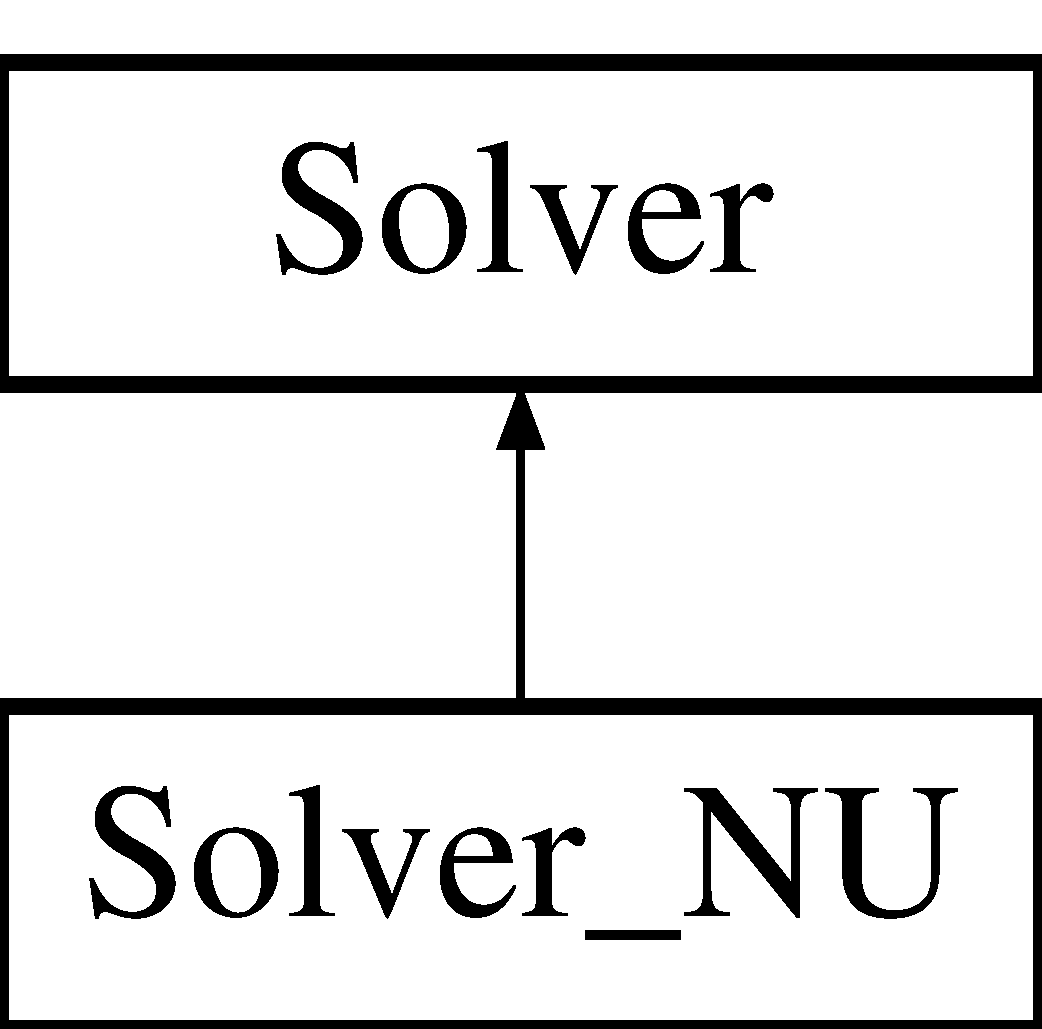
\includegraphics[height=2.000000cm]{classSolver__NU}
\end{center}
\end{figure}
\subsection*{Public Member Functions}
\begin{DoxyCompactItemize}
\item 
\hyperlink{classSolver__NU_a4f05e99c9939dcdf36840f27b1a9dde7}{Solver\+\_\+\+NU} ()
\item 
void \hyperlink{classSolver__NU_a3852f49023c0032934508156d7a9f132}{Solve} (int \hyperlink{classSolver_a88832d45b6de977b1cbb2afd4c0e494c}{l}, const \hyperlink{classQMatrix}{Q\+Matrix} \&\hyperlink{classSolver_a2d3461718f0570bdc47f5dfb31d61e0a}{Q}, const double $\ast$\hyperlink{classSolver_a882cce072f56679880d409e3e73f7ae8}{p}, const \hyperlink{svm__core_8cpp_a0fd9ce9d735064461bebfe6037026093}{schar} $\ast$\hyperlink{classSolver_a3acc1043d06dedf87f054ff3eea5c426}{y}, double $\ast$\hyperlink{classSolver_a00d7a7cefa2504d41c7db6cd7cc6b428}{alpha}, double \hyperlink{classSolver_a2e45dbea8be469bf8247e14768549dd5}{Cp}, double \hyperlink{classSolver_a38d741d194839fb445f982dd78e0b97b}{Cn}, double \hyperlink{classSolver_a718333cc2c1d40abf9c292a788cba1e5}{eps}, \hyperlink{structSolver_1_1SolutionInfo}{Solution\+Info} $\ast$si, int shrinking)
\end{DoxyCompactItemize}
\subsection*{Additional Inherited Members}


\subsection{Constructor \& Destructor Documentation}
\index{Solver\+\_\+\+NU@{Solver\+\_\+\+NU}!Solver\+\_\+\+NU@{Solver\+\_\+\+NU}}
\index{Solver\+\_\+\+NU@{Solver\+\_\+\+NU}!Solver\+\_\+\+NU@{Solver\+\_\+\+NU}}
\subsubsection[{Solver\+\_\+\+N\+U()}]{\setlength{\rightskip}{0pt plus 5cm}Solver\+\_\+\+N\+U\+::\+Solver\+\_\+\+NU (
\begin{DoxyParamCaption}
{}
\end{DoxyParamCaption}
)\hspace{0.3cm}{\ttfamily [inline]}}\hypertarget{classSolver__NU_a4f05e99c9939dcdf36840f27b1a9dde7}{}\label{classSolver__NU_a4f05e99c9939dcdf36840f27b1a9dde7}


\subsection{Member Function Documentation}
\index{Solver\+\_\+\+NU@{Solver\+\_\+\+NU}!Solve@{Solve}}
\index{Solve@{Solve}!Solver\+\_\+\+NU@{Solver\+\_\+\+NU}}
\subsubsection[{Solve(int l, const Q\+Matrix \&\+Q, const double $\ast$p, const schar $\ast$y, double $\ast$alpha, double Cp, double Cn, double eps, Solution\+Info $\ast$si, int shrinking)}]{\setlength{\rightskip}{0pt plus 5cm}void Solver\+\_\+\+N\+U\+::\+Solve (
\begin{DoxyParamCaption}
\item[{int}]{l, }
\item[{const {\bf Q\+Matrix} \&}]{Q, }
\item[{const double $\ast$}]{p, }
\item[{const {\bf schar} $\ast$}]{y, }
\item[{double $\ast$}]{alpha, }
\item[{double}]{Cp, }
\item[{double}]{Cn, }
\item[{double}]{eps, }
\item[{{\bf Solution\+Info} $\ast$}]{si, }
\item[{int}]{shrinking}
\end{DoxyParamCaption}
)\hspace{0.3cm}{\ttfamily [inline]}}\hypertarget{classSolver__NU_a3852f49023c0032934508156d7a9f132}{}\label{classSolver__NU_a3852f49023c0032934508156d7a9f132}


The documentation for this class was generated from the following file\+:\begin{DoxyCompactItemize}
\item 
src/\hyperlink{svm__core_8cpp}{svm\+\_\+core.\+cpp}\end{DoxyCompactItemize}

\hypertarget{classStates}{}\section{States Class Reference}
\label{classStates}\index{States@{States}}


{\ttfamily \#include $<$states.\+h$>$}

\subsection*{Public Member Functions}
\begin{DoxyCompactItemize}
\item 
\hyperlink{classStates_a77357dcd7269296068b166a86c035a4b}{States} ()
\item 
\hyperlink{classStates_a537d87c299ae42198d2f21f1bb046ec3}{$\sim$\+States} ()
\item 
int \hyperlink{classStates_ad6ea525e3db09581e11a80fac83201fd}{add\+\_\+states} (double st\mbox{[}$\,$\mbox{]}\mbox{[}\hyperlink{config_8h_a1d6565a8ececd15de44965eec4790919}{V\+A\+RS}\mbox{]}, int len)
\item 
int \hyperlink{classStates_a037a0060888bb6fc519783f3f06284f4}{traces\+\_\+num} ()
\item 
int \hyperlink{classStates_aff348a13a96c0699227f0dd49af5f51c}{size} ()
\item 
void \hyperlink{classStates_a25b5dab291f24971d9ddb1ff006a7cf4}{print\+\_\+trace} (int num)
\end{DoxyCompactItemize}
\subsection*{Data Fields}
\begin{DoxyCompactItemize}
\item 
double($\ast$ \hyperlink{classStates_a8b9a87b26c50e560d98c98d7e18f36b4}{values} )\mbox{[}\hyperlink{config_8h_a1d6565a8ececd15de44965eec4790919}{V\+A\+RS}\mbox{]}
\item 
int $\ast$ \hyperlink{classStates_ac7f438346962624026633389d156b5d0}{index}
\item 
int \hyperlink{classStates_a13e3842ad77b702e0f68cf875ded9534}{p\+\_\+index}
\item 
int \hyperlink{classStates_ab444a833f85348e8a850962da6c2c987}{label}
\end{DoxyCompactItemize}
\subsection*{Private Attributes}
\begin{DoxyCompactItemize}
\item 
int \hyperlink{classStates_a97d0d50850ab25e50914982341bba129}{max\+\_\+size}
\end{DoxyCompactItemize}
\subsection*{Friends}
\begin{DoxyCompactItemize}
\item 
std\+::ostream \& \hyperlink{classStates_a0a7f6b2b45f2366b0253093800b13fee}{operator$<$$<$} (std\+::ostream \&out, const \hyperlink{classStates}{States} \&ss)
\end{DoxyCompactItemize}


\subsection{Constructor \& Destructor Documentation}
\index{States@{States}!States@{States}}
\index{States@{States}!States@{States}}
\subsubsection[{States()}]{\setlength{\rightskip}{0pt plus 5cm}States\+::\+States (
\begin{DoxyParamCaption}
{}
\end{DoxyParamCaption}
)}\hypertarget{classStates_a77357dcd7269296068b166a86c035a4b}{}\label{classStates_a77357dcd7269296068b166a86c035a4b}
\index{States@{States}!````~States@{$\sim$\+States}}
\index{````~States@{$\sim$\+States}!States@{States}}
\subsubsection[{$\sim$\+States()}]{\setlength{\rightskip}{0pt plus 5cm}States\+::$\sim$\+States (
\begin{DoxyParamCaption}
{}
\end{DoxyParamCaption}
)}\hypertarget{classStates_a537d87c299ae42198d2f21f1bb046ec3}{}\label{classStates_a537d87c299ae42198d2f21f1bb046ec3}


\subsection{Member Function Documentation}
\index{States@{States}!add\+\_\+states@{add\+\_\+states}}
\index{add\+\_\+states@{add\+\_\+states}!States@{States}}
\subsubsection[{add\+\_\+states(double st[][V\+A\+RS], int len)}]{\setlength{\rightskip}{0pt plus 5cm}int States\+::add\+\_\+states (
\begin{DoxyParamCaption}
\item[{double}]{st\mbox{[}$\,$\mbox{]}\mbox{[}\+V\+A\+R\+S\mbox{]}, }
\item[{int}]{len}
\end{DoxyParamCaption}
)}\hypertarget{classStates_ad6ea525e3db09581e11a80fac83201fd}{}\label{classStates_ad6ea525e3db09581e11a80fac83201fd}
\index{States@{States}!print\+\_\+trace@{print\+\_\+trace}}
\index{print\+\_\+trace@{print\+\_\+trace}!States@{States}}
\subsubsection[{print\+\_\+trace(int num)}]{\setlength{\rightskip}{0pt plus 5cm}void States\+::print\+\_\+trace (
\begin{DoxyParamCaption}
\item[{int}]{num}
\end{DoxyParamCaption}
)}\hypertarget{classStates_a25b5dab291f24971d9ddb1ff006a7cf4}{}\label{classStates_a25b5dab291f24971d9ddb1ff006a7cf4}
\index{States@{States}!size@{size}}
\index{size@{size}!States@{States}}
\subsubsection[{size()}]{\setlength{\rightskip}{0pt plus 5cm}int States\+::size (
\begin{DoxyParamCaption}
{}
\end{DoxyParamCaption}
)}\hypertarget{classStates_aff348a13a96c0699227f0dd49af5f51c}{}\label{classStates_aff348a13a96c0699227f0dd49af5f51c}
\index{States@{States}!traces\+\_\+num@{traces\+\_\+num}}
\index{traces\+\_\+num@{traces\+\_\+num}!States@{States}}
\subsubsection[{traces\+\_\+num()}]{\setlength{\rightskip}{0pt plus 5cm}int States\+::traces\+\_\+num (
\begin{DoxyParamCaption}
{}
\end{DoxyParamCaption}
)}\hypertarget{classStates_a037a0060888bb6fc519783f3f06284f4}{}\label{classStates_a037a0060888bb6fc519783f3f06284f4}


\subsection{Friends And Related Function Documentation}
\index{States@{States}!operator$<$$<$@{operator$<$$<$}}
\index{operator$<$$<$@{operator$<$$<$}!States@{States}}
\subsubsection[{operator$<$$<$}]{\setlength{\rightskip}{0pt plus 5cm}std\+::ostream\& operator$<$$<$ (
\begin{DoxyParamCaption}
\item[{std\+::ostream \&}]{out, }
\item[{const {\bf States} \&}]{ss}
\end{DoxyParamCaption}
)\hspace{0.3cm}{\ttfamily [friend]}}\hypertarget{classStates_a0a7f6b2b45f2366b0253093800b13fee}{}\label{classStates_a0a7f6b2b45f2366b0253093800b13fee}


\subsection{Field Documentation}
\index{States@{States}!index@{index}}
\index{index@{index}!States@{States}}
\subsubsection[{index}]{\setlength{\rightskip}{0pt plus 5cm}int$\ast$ States\+::index}\hypertarget{classStates_ac7f438346962624026633389d156b5d0}{}\label{classStates_ac7f438346962624026633389d156b5d0}
\index{States@{States}!label@{label}}
\index{label@{label}!States@{States}}
\subsubsection[{label}]{\setlength{\rightskip}{0pt plus 5cm}int States\+::label}\hypertarget{classStates_ab444a833f85348e8a850962da6c2c987}{}\label{classStates_ab444a833f85348e8a850962da6c2c987}
\index{States@{States}!max\+\_\+size@{max\+\_\+size}}
\index{max\+\_\+size@{max\+\_\+size}!States@{States}}
\subsubsection[{max\+\_\+size}]{\setlength{\rightskip}{0pt plus 5cm}int States\+::max\+\_\+size\hspace{0.3cm}{\ttfamily [private]}}\hypertarget{classStates_a97d0d50850ab25e50914982341bba129}{}\label{classStates_a97d0d50850ab25e50914982341bba129}
\index{States@{States}!p\+\_\+index@{p\+\_\+index}}
\index{p\+\_\+index@{p\+\_\+index}!States@{States}}
\subsubsection[{p\+\_\+index}]{\setlength{\rightskip}{0pt plus 5cm}int States\+::p\+\_\+index}\hypertarget{classStates_a13e3842ad77b702e0f68cf875ded9534}{}\label{classStates_a13e3842ad77b702e0f68cf875ded9534}
\index{States@{States}!values@{values}}
\index{values@{values}!States@{States}}
\subsubsection[{values}]{\setlength{\rightskip}{0pt plus 5cm}double($\ast$ States\+::values)\mbox{[}{\bf V\+A\+RS}\mbox{]}}\hypertarget{classStates_a8b9a87b26c50e560d98c98d7e18f36b4}{}\label{classStates_a8b9a87b26c50e560d98c98d7e18f36b4}


The documentation for this class was generated from the following files\+:\begin{DoxyCompactItemize}
\item 
include/\hyperlink{states_8h}{states.\+h}\item 
src/\hyperlink{states_8cpp}{states.\+cpp}\end{DoxyCompactItemize}

\hypertarget{classSVC__Q}{}\section{S\+V\+C\+\_\+Q Class Reference}
\label{classSVC__Q}\index{S\+V\+C\+\_\+Q@{S\+V\+C\+\_\+Q}}
Inheritance diagram for S\+V\+C\+\_\+Q\+:\begin{figure}[H]
\begin{center}
\leavevmode
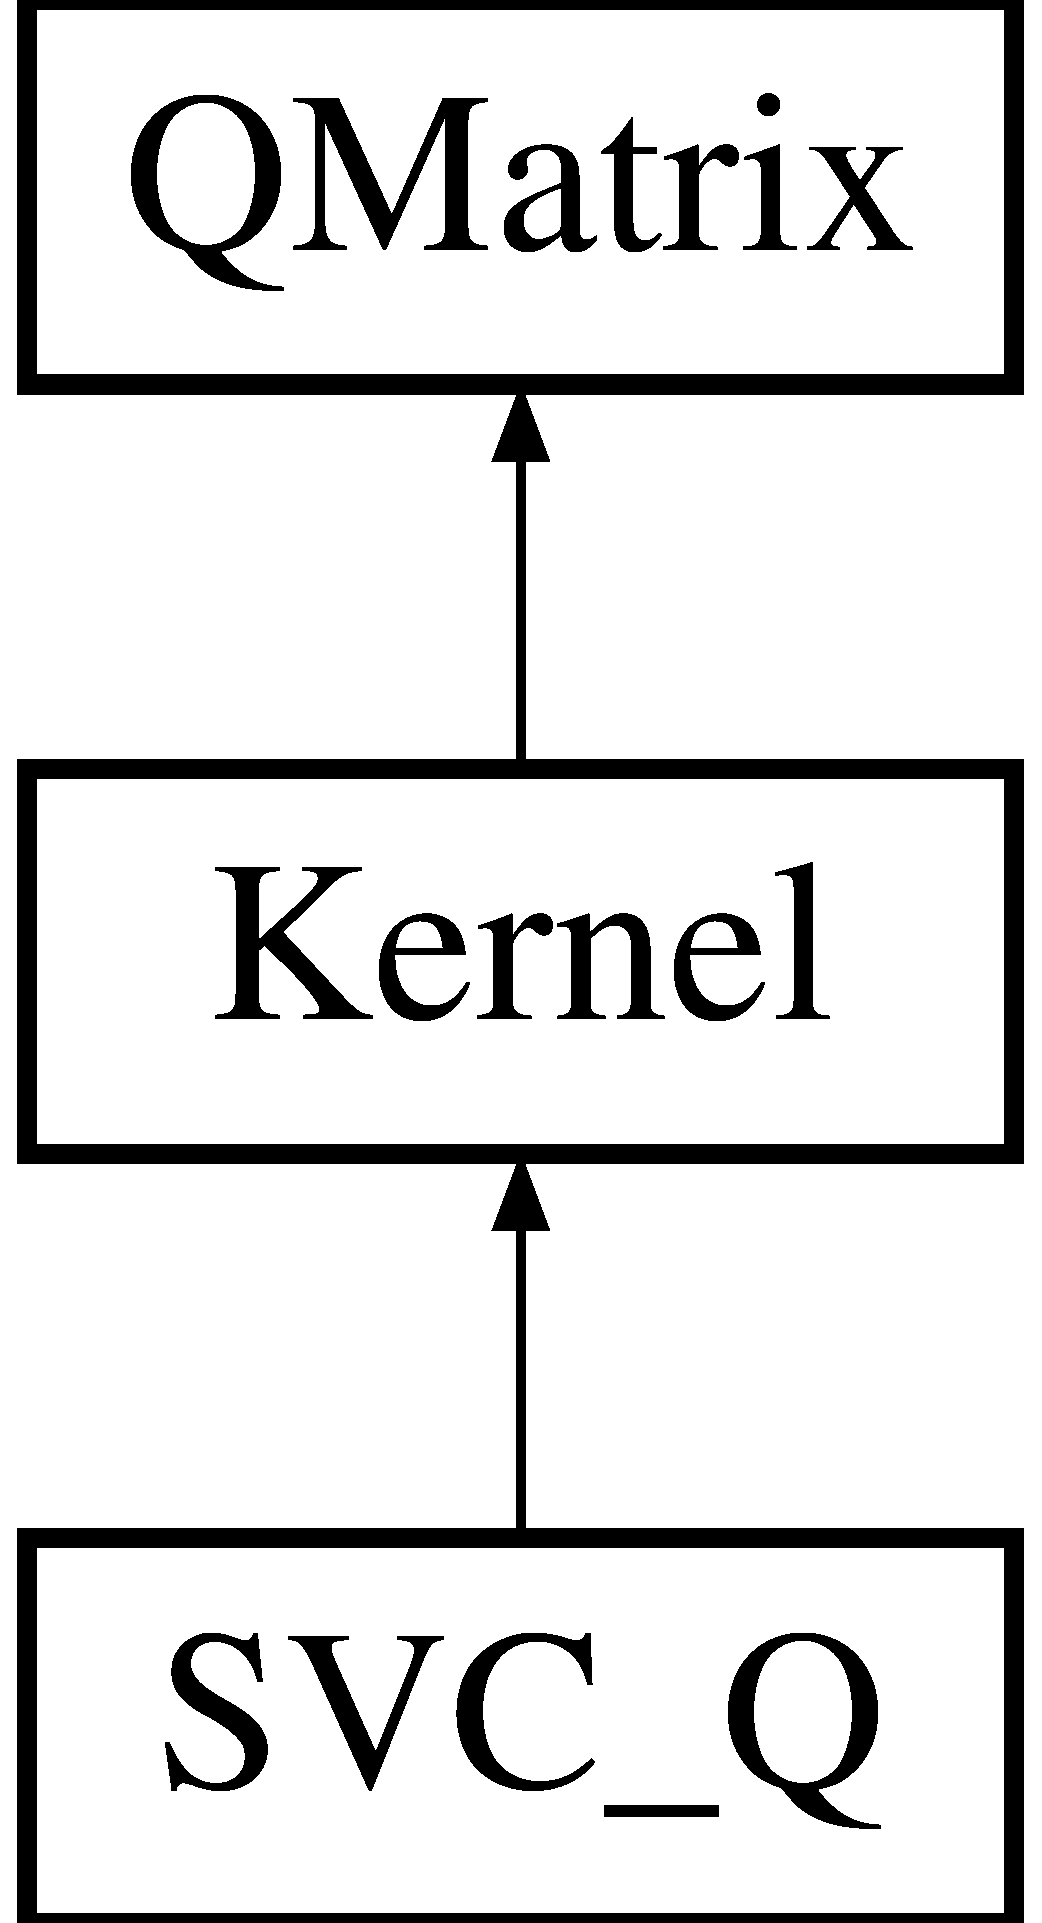
\includegraphics[height=3.000000cm]{classSVC__Q}
\end{center}
\end{figure}
\subsection*{Public Member Functions}
\begin{DoxyCompactItemize}
\item 
\hyperlink{classSVC__Q_a23d7cf0b0606ccf2cb987205b94dddc7}{S\+V\+C\+\_\+Q} (const \hyperlink{structsvm__problem}{svm\+\_\+problem} \&prob, const \hyperlink{structsvm__parameter}{svm\+\_\+parameter} \&param, const \hyperlink{svm__core_8cpp_a0fd9ce9d735064461bebfe6037026093}{schar} $\ast$y\+\_\+)
\item 
\hyperlink{svm__core_8cpp_a8755d90a54ecfb8d15051af3e0542592}{Qfloat} $\ast$ \hyperlink{classSVC__Q_a9341b6030b3fdc88466e4a602b5abff0}{get\+\_\+Q} (int i, int len) const 
\item 
double $\ast$ \hyperlink{classSVC__Q_ac73020a6e438e209d63223e1fa8cac29}{get\+\_\+\+QD} () const 
\item 
void \hyperlink{classSVC__Q_a9c889db8ee0156ed5bcdaa4d6bc4e245}{swap\+\_\+index} (int i, int j) const 
\item 
\hyperlink{classSVC__Q_af491500a4a6e2df46083098ee3397142}{$\sim$\+S\+V\+C\+\_\+Q} ()
\end{DoxyCompactItemize}
\subsection*{Additional Inherited Members}


\subsection{Constructor \& Destructor Documentation}
\index{S\+V\+C\+\_\+Q@{S\+V\+C\+\_\+Q}!S\+V\+C\+\_\+Q@{S\+V\+C\+\_\+Q}}
\index{S\+V\+C\+\_\+Q@{S\+V\+C\+\_\+Q}!S\+V\+C\+\_\+Q@{S\+V\+C\+\_\+Q}}
\subsubsection[{S\+V\+C\+\_\+\+Q(const svm\+\_\+problem \&prob, const svm\+\_\+parameter \&param, const schar $\ast$y\+\_\+)}]{\setlength{\rightskip}{0pt plus 5cm}S\+V\+C\+\_\+\+Q\+::\+S\+V\+C\+\_\+Q (
\begin{DoxyParamCaption}
\item[{const {\bf svm\+\_\+problem} \&}]{prob, }
\item[{const {\bf svm\+\_\+parameter} \&}]{param, }
\item[{const {\bf schar} $\ast$}]{y\+\_\+}
\end{DoxyParamCaption}
)\hspace{0.3cm}{\ttfamily [inline]}}\hypertarget{classSVC__Q_a23d7cf0b0606ccf2cb987205b94dddc7}{}\label{classSVC__Q_a23d7cf0b0606ccf2cb987205b94dddc7}
\index{S\+V\+C\+\_\+Q@{S\+V\+C\+\_\+Q}!````~S\+V\+C\+\_\+Q@{$\sim$\+S\+V\+C\+\_\+Q}}
\index{````~S\+V\+C\+\_\+Q@{$\sim$\+S\+V\+C\+\_\+Q}!S\+V\+C\+\_\+Q@{S\+V\+C\+\_\+Q}}
\subsubsection[{$\sim$\+S\+V\+C\+\_\+\+Q()}]{\setlength{\rightskip}{0pt plus 5cm}S\+V\+C\+\_\+\+Q\+::$\sim$\+S\+V\+C\+\_\+Q (
\begin{DoxyParamCaption}
{}
\end{DoxyParamCaption}
)\hspace{0.3cm}{\ttfamily [inline]}}\hypertarget{classSVC__Q_af491500a4a6e2df46083098ee3397142}{}\label{classSVC__Q_af491500a4a6e2df46083098ee3397142}


\subsection{Member Function Documentation}
\index{S\+V\+C\+\_\+Q@{S\+V\+C\+\_\+Q}!get\+\_\+Q@{get\+\_\+Q}}
\index{get\+\_\+Q@{get\+\_\+Q}!S\+V\+C\+\_\+Q@{S\+V\+C\+\_\+Q}}
\subsubsection[{get\+\_\+\+Q(int i, int len) const }]{\setlength{\rightskip}{0pt plus 5cm}{\bf Qfloat}$\ast$ S\+V\+C\+\_\+\+Q\+::get\+\_\+Q (
\begin{DoxyParamCaption}
\item[{int}]{i, }
\item[{int}]{len}
\end{DoxyParamCaption}
) const\hspace{0.3cm}{\ttfamily [inline]}, {\ttfamily [virtual]}}\hypertarget{classSVC__Q_a9341b6030b3fdc88466e4a602b5abff0}{}\label{classSVC__Q_a9341b6030b3fdc88466e4a602b5abff0}


Implements \hyperlink{classKernel_a02f328649424359b92b941f5219a6060}{Kernel}.

\index{S\+V\+C\+\_\+Q@{S\+V\+C\+\_\+Q}!get\+\_\+\+QD@{get\+\_\+\+QD}}
\index{get\+\_\+\+QD@{get\+\_\+\+QD}!S\+V\+C\+\_\+Q@{S\+V\+C\+\_\+Q}}
\subsubsection[{get\+\_\+\+Q\+D() const }]{\setlength{\rightskip}{0pt plus 5cm}double$\ast$ S\+V\+C\+\_\+\+Q\+::get\+\_\+\+QD (
\begin{DoxyParamCaption}
{}
\end{DoxyParamCaption}
) const\hspace{0.3cm}{\ttfamily [inline]}, {\ttfamily [virtual]}}\hypertarget{classSVC__Q_ac73020a6e438e209d63223e1fa8cac29}{}\label{classSVC__Q_ac73020a6e438e209d63223e1fa8cac29}


Implements \hyperlink{classKernel_a7bf9602583da1af48d15d19da69514ac}{Kernel}.

\index{S\+V\+C\+\_\+Q@{S\+V\+C\+\_\+Q}!swap\+\_\+index@{swap\+\_\+index}}
\index{swap\+\_\+index@{swap\+\_\+index}!S\+V\+C\+\_\+Q@{S\+V\+C\+\_\+Q}}
\subsubsection[{swap\+\_\+index(int i, int j) const }]{\setlength{\rightskip}{0pt plus 5cm}void S\+V\+C\+\_\+\+Q\+::swap\+\_\+index (
\begin{DoxyParamCaption}
\item[{int}]{i, }
\item[{int}]{j}
\end{DoxyParamCaption}
) const\hspace{0.3cm}{\ttfamily [inline]}, {\ttfamily [virtual]}}\hypertarget{classSVC__Q_a9c889db8ee0156ed5bcdaa4d6bc4e245}{}\label{classSVC__Q_a9c889db8ee0156ed5bcdaa4d6bc4e245}


Reimplemented from \hyperlink{classKernel_adca807c5584bc42fd098cd9eb1f19621}{Kernel}.



The documentation for this class was generated from the following file\+:\begin{DoxyCompactItemize}
\item 
src/\hyperlink{svm__core_8cpp}{svm\+\_\+core.\+cpp}\end{DoxyCompactItemize}

\hypertarget{classSVM}{}\section{S\+VM Class Reference}
\label{classSVM}\index{S\+VM@{S\+VM}}


{\ttfamily \#include $<$svm.\+h$>$}

Inheritance diagram for S\+VM\+:\begin{figure}[H]
\begin{center}
\leavevmode
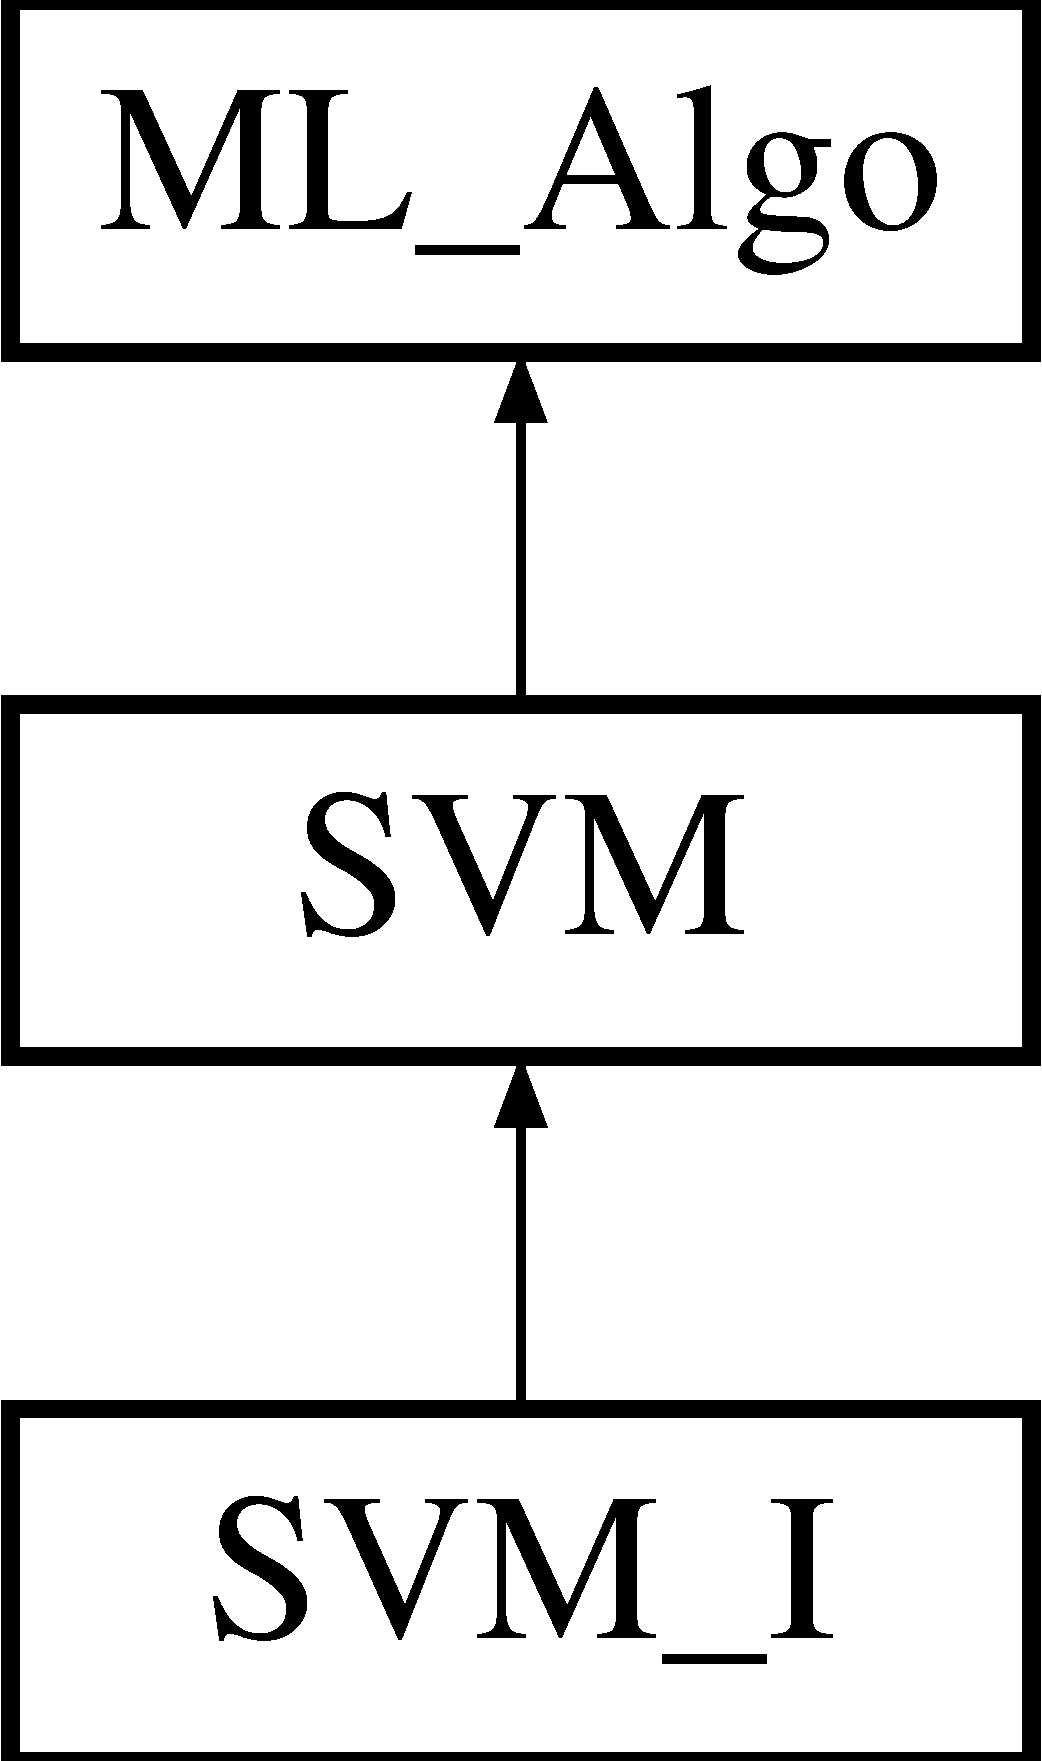
\includegraphics[height=3.000000cm]{classSVM}
\end{center}
\end{figure}
\subsection*{Public Member Functions}
\begin{DoxyCompactItemize}
\item 
\hyperlink{classSVM_ad8716b6d07bd35810f62662856af3a09}{S\+VM} (void($\ast$f)(const char $\ast$)=N\+U\+LL, int \hyperlink{classSVM_a4563cef982f6e1c67acf0c7b0ec8909b}{size}=10000)
\item 
virtual \hyperlink{classSVM_ad2a87ef0f940145f04150e9561f10478}{$\sim$\+S\+VM} ()
\item 
virtual int \hyperlink{classSVM_a930fe217e3affd64acb6700f5f8082e1}{prepare\+\_\+training\+\_\+data} (\hyperlink{classStates}{States} $\ast$gsets, int \&pre\+\_\+positive\+\_\+size, int \&pre\+\_\+negative\+\_\+size)
\begin{DoxyCompactList}\small\item\em init training data method. This should be called before any training happens. \end{DoxyCompactList}\item 
virtual int \hyperlink{classSVM_a6a1d895b86522eab683d66ded4d3a049}{train} ()
\begin{DoxyCompactList}\small\item\em The most important T\+R\+A\+IN method, which calls real training algorithm to do training. \end{DoxyCompactList}\item 
virtual double \hyperlink{classSVM_af208fc653a382591f20c0fcf7a186362}{predict\+\_\+on\+\_\+training\+\_\+set} ()
\begin{DoxyCompactList}\small\item\em Calculate the predict precision of the training-\/model on the training set. \end{DoxyCompactList}\item 
virtual int \hyperlink{classSVM_aa610ec08173c8603ad6e02f26cbe8e1c}{check\+\_\+question\+\_\+set} (\hyperlink{classStates}{States} \&qset)
\begin{DoxyCompactList}\small\item\em test on question state sets to see if there is an invalidation \end{DoxyCompactList}\item 
virtual int \hyperlink{classSVM_a712dcd7cb65a8045a77dd474869dd5c4}{get\+\_\+converged} (\hyperlink{classEquation}{Equation} $\ast$, int)
\begin{DoxyCompactList}\small\item\em check whether the training is converged or not \end{DoxyCompactList}\item 
virtual std\+::ostream \& \hyperlink{classSVM_a6e5a3fbae4da1ecd4773173a2b590c21}{\+\_\+print} (std\+::ostream \&out) const 
\begin{DoxyCompactList}\small\item\em This is the function really called to output this object. We involve this as to support polymophism for operator $<$$<$. \end{DoxyCompactList}\item 
virtual int \hyperlink{classSVM_a4563cef982f6e1c67acf0c7b0ec8909b}{size} ()
\begin{DoxyCompactList}\small\item\em This method returns the current problem size (the number of training states). \end{DoxyCompactList}\item 
virtual \hyperlink{classEquation}{Equation} $\ast$ \hyperlink{classSVM_abd2d511c6cb9f64a29a4551f6435bfd2}{roundoff} (int \&num)
\begin{DoxyCompactList}\small\item\em Round off the whole training model.(equations) \end{DoxyCompactList}\item 
virtual int \hyperlink{classSVM_a972215d3c749ba550c85763c8871567f}{predict} (double $\ast$v, int label=0)
\begin{DoxyCompactList}\small\item\em Predict sample x against the whole training model.(equations) \end{DoxyCompactList}\end{DoxyCompactItemize}
\subsection*{Data Fields}
\begin{DoxyCompactItemize}
\item 
\hyperlink{structsvm__model}{svm\+\_\+model} $\ast$ \hyperlink{classSVM_a546f3dfe2004cbf9096105a67b0a0e66}{model}
\item 
\hyperlink{classEquation}{Equation} $\ast$ \hyperlink{classSVM_ae7e7d62512de9800ea1c47fc7ad33adc}{main\+\_\+equation}
\item 
\hyperlink{structsvm__parameter}{svm\+\_\+parameter} \hyperlink{classSVM_ad28af66070f8e9f9f6c74132c78aa245}{param}
\item 
\hyperlink{structsvm__problem}{svm\+\_\+problem} \hyperlink{classSVM_a154369e018e4f487838709b350474bc6}{problem}
\item 
double $\ast$ \hyperlink{classSVM_a4a2cfc7a3b8b1e65a8edd81ffc0985ba}{training\+\_\+label}
\item 
double $\ast$$\ast$ \hyperlink{classSVM_a0d63a10c574ace471efcd8e6553b7bd9}{training\+\_\+set}
\end{DoxyCompactItemize}
\subsection*{Protected Attributes}
\begin{DoxyCompactItemize}
\item 
int \hyperlink{classSVM_a0d910cf52a7891bec9d3f668cc819210}{max\+\_\+size}
\end{DoxyCompactItemize}
\subsection*{Friends}
\begin{DoxyCompactItemize}
\item 
std\+::ostream \& \hyperlink{classSVM_af21f811318dedf7522a8f48741a1d979}{operator$<$$<$} (std\+::ostream \&out, const \hyperlink{classSVM}{S\+VM} \&svm)
\end{DoxyCompactItemize}


\subsection{Constructor \& Destructor Documentation}
\index{S\+VM@{S\+VM}!S\+VM@{S\+VM}}
\index{S\+VM@{S\+VM}!S\+VM@{S\+VM}}
\subsubsection[{S\+V\+M(void($\ast$f)(const char $\ast$)=\+N\+U\+L\+L, int size=10000)}]{\setlength{\rightskip}{0pt plus 5cm}S\+V\+M\+::\+S\+VM (
\begin{DoxyParamCaption}
\item[{void($\ast$)(const char $\ast$)}]{f = {\ttfamily NULL}, }
\item[{int}]{size = {\ttfamily 10000}}
\end{DoxyParamCaption}
)}\hypertarget{classSVM_ad8716b6d07bd35810f62662856af3a09}{}\label{classSVM_ad8716b6d07bd35810f62662856af3a09}
\index{S\+VM@{S\+VM}!````~S\+VM@{$\sim$\+S\+VM}}
\index{````~S\+VM@{$\sim$\+S\+VM}!S\+VM@{S\+VM}}
\subsubsection[{$\sim$\+S\+V\+M()}]{\setlength{\rightskip}{0pt plus 5cm}S\+V\+M\+::$\sim$\+S\+VM (
\begin{DoxyParamCaption}
{}
\end{DoxyParamCaption}
)\hspace{0.3cm}{\ttfamily [virtual]}}\hypertarget{classSVM_ad2a87ef0f940145f04150e9561f10478}{}\label{classSVM_ad2a87ef0f940145f04150e9561f10478}


\subsection{Member Function Documentation}
\index{S\+VM@{S\+VM}!\+\_\+print@{\+\_\+print}}
\index{\+\_\+print@{\+\_\+print}!S\+VM@{S\+VM}}
\subsubsection[{\+\_\+print(std\+::ostream \&out) const }]{\setlength{\rightskip}{0pt plus 5cm}std\+::ostream \& S\+V\+M\+::\+\_\+print (
\begin{DoxyParamCaption}
\item[{std\+::ostream \&}]{out}
\end{DoxyParamCaption}
) const\hspace{0.3cm}{\ttfamily [virtual]}}\hypertarget{classSVM_a6e5a3fbae4da1ecd4773173a2b590c21}{}\label{classSVM_a6e5a3fbae4da1ecd4773173a2b590c21}


This is the function really called to output this object. We involve this as to support polymophism for operator $<$$<$. 



Reimplemented from \hyperlink{classML__Algo_ad689e5642c5db0971c53909b52cc67d4}{M\+L\+\_\+\+Algo}.



Reimplemented in \hyperlink{classSVM__I_ab0ae30d86d9f9026908a7b902f7a78e3}{S\+V\+M\+\_\+I}.

\index{S\+VM@{S\+VM}!check\+\_\+question\+\_\+set@{check\+\_\+question\+\_\+set}}
\index{check\+\_\+question\+\_\+set@{check\+\_\+question\+\_\+set}!S\+VM@{S\+VM}}
\subsubsection[{check\+\_\+question\+\_\+set(\+States \&qset)}]{\setlength{\rightskip}{0pt plus 5cm}int S\+V\+M\+::check\+\_\+question\+\_\+set (
\begin{DoxyParamCaption}
\item[{{\bf States} \&}]{qset}
\end{DoxyParamCaption}
)\hspace{0.3cm}{\ttfamily [virtual]}}\hypertarget{classSVM_aa610ec08173c8603ad6e02f26cbe8e1c}{}\label{classSVM_aa610ec08173c8603ad6e02f26cbe8e1c}


test on question state sets to see if there is an invalidation 

The method will output the inforamtion if a question trace invalidate the training model


\begin{DoxyParams}{Parameters}
{\em qset} & is a reference type to question states. \\
\hline
\end{DoxyParams}
\begin{DoxyReturn}{Returns}
int 0 if no error 
\end{DoxyReturn}


Implements \hyperlink{classML__Algo_a4d757e7fb178ce41ec713bcd84807d33}{M\+L\+\_\+\+Algo}.



Reimplemented in \hyperlink{classSVM__I_a84470dce77add6377454c4408c6c1466}{S\+V\+M\+\_\+I}.

\index{S\+VM@{S\+VM}!get\+\_\+converged@{get\+\_\+converged}}
\index{get\+\_\+converged@{get\+\_\+converged}!S\+VM@{S\+VM}}
\subsubsection[{get\+\_\+converged(\+Equation $\ast$, int)}]{\setlength{\rightskip}{0pt plus 5cm}int S\+V\+M\+::get\+\_\+converged (
\begin{DoxyParamCaption}
\item[{{\bf Equation} $\ast$}]{previous\+\_\+equations, }
\item[{int}]{equation\+\_\+num}
\end{DoxyParamCaption}
)\hspace{0.3cm}{\ttfamily [virtual]}}\hypertarget{classSVM_a712dcd7cb65a8045a77dd474869dd5c4}{}\label{classSVM_a712dcd7cb65a8045a77dd474869dd5c4}


check whether the training is converged or not 

current\+\_\+training\+\_\+equations $\sim$= previous\+\_\+trainig\+\_\+equations ???


\begin{DoxyParams}{Parameters}
{\em previous\+\_\+equations} & contains all the equation we get from last trainig session. \\
\hline
{\em equation\+\_\+num} & is the number of equations get from last training session \\
\hline
\end{DoxyParams}
\begin{DoxyReturn}{Returns}
int 0 if converged 
\end{DoxyReturn}


Implements \hyperlink{classML__Algo_a3d2c7bfa53c13005dfde112c9e473c5e}{M\+L\+\_\+\+Algo}.



Reimplemented in \hyperlink{classSVM__I_a5d1a8c93d41597aea5f31689687dbc77}{S\+V\+M\+\_\+I}.

\index{S\+VM@{S\+VM}!predict@{predict}}
\index{predict@{predict}!S\+VM@{S\+VM}}
\subsubsection[{predict(double $\ast$v, int label=0)}]{\setlength{\rightskip}{0pt plus 5cm}int S\+V\+M\+::predict (
\begin{DoxyParamCaption}
\item[{double $\ast$}]{x, }
\item[{int}]{flag = {\ttfamily 0}}
\end{DoxyParamCaption}
)\hspace{0.3cm}{\ttfamily [virtual]}}\hypertarget{classSVM_a972215d3c749ba550c85763c8871567f}{}\label{classSVM_a972215d3c749ba550c85763c8871567f}


Predict sample x against the whole training model.(equations) 


\begin{DoxyParams}{Parameters}
{\em x} & contains the sample to be tested. \\
\hline
{\em flag} & leave this to be Z\+E\+RO... \\
\hline
\end{DoxyParams}
\begin{DoxyReturn}{Returns}
The label of prediction 
\end{DoxyReturn}


Implements \hyperlink{classML__Algo_aae12eabc95fd3eb5305f1ae7a14e0193}{M\+L\+\_\+\+Algo}.



Reimplemented in \hyperlink{classSVM__I_abe0a76aa6d31d18c2ee66002c35c813f}{S\+V\+M\+\_\+I}.

\index{S\+VM@{S\+VM}!predict\+\_\+on\+\_\+training\+\_\+set@{predict\+\_\+on\+\_\+training\+\_\+set}}
\index{predict\+\_\+on\+\_\+training\+\_\+set@{predict\+\_\+on\+\_\+training\+\_\+set}!S\+VM@{S\+VM}}
\subsubsection[{predict\+\_\+on\+\_\+training\+\_\+set()}]{\setlength{\rightskip}{0pt plus 5cm}double S\+V\+M\+::predict\+\_\+on\+\_\+training\+\_\+set (
\begin{DoxyParamCaption}
{}
\end{DoxyParamCaption}
)\hspace{0.3cm}{\ttfamily [virtual]}}\hypertarget{classSVM_af208fc653a382591f20c0fcf7a186362}{}\label{classSVM_af208fc653a382591f20c0fcf7a186362}


Calculate the predict precision of the training-\/model on the training set. 

\begin{DoxyReturn}{Returns}
double Return precision we can get. Should be a value between 0 and 1. 
\end{DoxyReturn}


Implements \hyperlink{classML__Algo_a39dd640e7c910becf611b9265843ac77}{M\+L\+\_\+\+Algo}.



Reimplemented in \hyperlink{classSVM__I_a643c2a6e58f8e70ab276ade9b1873bf6}{S\+V\+M\+\_\+I}.

\index{S\+VM@{S\+VM}!prepare\+\_\+training\+\_\+data@{prepare\+\_\+training\+\_\+data}}
\index{prepare\+\_\+training\+\_\+data@{prepare\+\_\+training\+\_\+data}!S\+VM@{S\+VM}}
\subsubsection[{prepare\+\_\+training\+\_\+data(\+States $\ast$gsets, int \&pre\+\_\+positive\+\_\+size, int \&pre\+\_\+negative\+\_\+size)}]{\setlength{\rightskip}{0pt plus 5cm}int S\+V\+M\+::prepare\+\_\+training\+\_\+data (
\begin{DoxyParamCaption}
\item[{{\bf States} $\ast$}]{gsets, }
\item[{int \&}]{pre\+\_\+positive\+\_\+size, }
\item[{int \&}]{pre\+\_\+negative\+\_\+size}
\end{DoxyParamCaption}
)\hspace{0.3cm}{\ttfamily [virtual]}}\hypertarget{classSVM_a930fe217e3affd64acb6700f5f8082e1}{}\label{classSVM_a930fe217e3affd64acb6700f5f8082e1}


init training data method. This should be called before any training happens. 


\begin{DoxyParams}{Parameters}
{\em gsets} & The states array to store all the generated states information. The size must be 4, and index -\/1 should be accessible \\
\hline
{\em pre\+\_\+positive\+\_\+size} & This records the last positive size of states. And also set by callee to the new value Initially set to 0, as there is no elements in positive states. Calls afterwards should pass the value set by last call. \\
\hline
{\em pre\+\_\+negative\+\_\+size} & This records the last negative size of states. And also set by callee to the new value Initially set to 0, as there is no elements in positive states. Calls afterwards should pass the value set by last call. \\
\hline
\end{DoxyParams}
\begin{DoxyReturn}{Returns}
int 0 if no error 
\end{DoxyReturn}


Implements \hyperlink{classML__Algo_ab98458d234bdf97c2ed678030d90c513}{M\+L\+\_\+\+Algo}.



Reimplemented in \hyperlink{classSVM__I_ab0236699daa4967cfec71234faa785c5}{S\+V\+M\+\_\+I}.

\index{S\+VM@{S\+VM}!roundoff@{roundoff}}
\index{roundoff@{roundoff}!S\+VM@{S\+VM}}
\subsubsection[{roundoff(int \&num)}]{\setlength{\rightskip}{0pt plus 5cm}{\bf Equation} $\ast$ S\+V\+M\+::roundoff (
\begin{DoxyParamCaption}
\item[{int \&}]{equation\+\_\+num}
\end{DoxyParamCaption}
)\hspace{0.3cm}{\ttfamily [virtual]}}\hypertarget{classSVM_abd2d511c6cb9f64a29a4551f6435bfd2}{}\label{classSVM_abd2d511c6cb9f64a29a4551f6435bfd2}


Round off the whole training model.(equations) 


\begin{DoxyParams}{Parameters}
{\em equation\+\_\+num} & set by callee to notify the number of equations we currently get \\
\hline
\end{DoxyParams}
\begin{DoxyReturn}{Returns}
Eqation Point the rounded off equations. Remember to D\+E\+L\+E\+TE them after use by caller. Otherwise memory leak. 
\end{DoxyReturn}


Implements \hyperlink{classML__Algo_a398214e0462ebfdde10e745240030a34}{M\+L\+\_\+\+Algo}.



Reimplemented in \hyperlink{classSVM__I_a91b713ef0810fd4c83a5c711aea9fecf}{S\+V\+M\+\_\+I}.

\index{S\+VM@{S\+VM}!size@{size}}
\index{size@{size}!S\+VM@{S\+VM}}
\subsubsection[{size()}]{\setlength{\rightskip}{0pt plus 5cm}int S\+V\+M\+::size (
\begin{DoxyParamCaption}
{}
\end{DoxyParamCaption}
)\hspace{0.3cm}{\ttfamily [virtual]}}\hypertarget{classSVM_a4563cef982f6e1c67acf0c7b0ec8909b}{}\label{classSVM_a4563cef982f6e1c67acf0c7b0ec8909b}


This method returns the current problem size (the number of training states). 

\begin{DoxyReturn}{Returns}
int the size of problem 
\end{DoxyReturn}


Implements \hyperlink{classML__Algo_a8650c3894c1992492f8bc86edf1b3ffd}{M\+L\+\_\+\+Algo}.



Reimplemented in \hyperlink{classSVM__I_a1b66cefe313cffaa77d4271dfb4b8474}{S\+V\+M\+\_\+I}.

\index{S\+VM@{S\+VM}!train@{train}}
\index{train@{train}!S\+VM@{S\+VM}}
\subsubsection[{train()}]{\setlength{\rightskip}{0pt plus 5cm}int S\+V\+M\+::train (
\begin{DoxyParamCaption}
{}
\end{DoxyParamCaption}
)\hspace{0.3cm}{\ttfamily [virtual]}}\hypertarget{classSVM_a6a1d895b86522eab683d66ded4d3a049}{}\label{classSVM_a6a1d895b86522eab683d66ded4d3a049}


The most important T\+R\+A\+IN method, which calls real training algorithm to do training. 

\begin{DoxyReturn}{Returns}
int 0 if no error. 
\end{DoxyReturn}


Implements \hyperlink{classML__Algo_a0a5d241191d4249c60a40d966fb19aee}{M\+L\+\_\+\+Algo}.



Reimplemented in \hyperlink{classSVM__I_abf732821c264b2cb8bef5d252991f2b6}{S\+V\+M\+\_\+I}.



\subsection{Friends And Related Function Documentation}
\index{S\+VM@{S\+VM}!operator$<$$<$@{operator$<$$<$}}
\index{operator$<$$<$@{operator$<$$<$}!S\+VM@{S\+VM}}
\subsubsection[{operator$<$$<$}]{\setlength{\rightskip}{0pt plus 5cm}std\+::ostream\& operator$<$$<$ (
\begin{DoxyParamCaption}
\item[{std\+::ostream \&}]{out, }
\item[{const {\bf S\+VM} \&}]{svm}
\end{DoxyParamCaption}
)\hspace{0.3cm}{\ttfamily [friend]}}\hypertarget{classSVM_af21f811318dedf7522a8f48741a1d979}{}\label{classSVM_af21f811318dedf7522a8f48741a1d979}


\subsection{Field Documentation}
\index{S\+VM@{S\+VM}!main\+\_\+equation@{main\+\_\+equation}}
\index{main\+\_\+equation@{main\+\_\+equation}!S\+VM@{S\+VM}}
\subsubsection[{main\+\_\+equation}]{\setlength{\rightskip}{0pt plus 5cm}{\bf Equation}$\ast$ S\+V\+M\+::main\+\_\+equation}\hypertarget{classSVM_ae7e7d62512de9800ea1c47fc7ad33adc}{}\label{classSVM_ae7e7d62512de9800ea1c47fc7ad33adc}
\index{S\+VM@{S\+VM}!max\+\_\+size@{max\+\_\+size}}
\index{max\+\_\+size@{max\+\_\+size}!S\+VM@{S\+VM}}
\subsubsection[{max\+\_\+size}]{\setlength{\rightskip}{0pt plus 5cm}int S\+V\+M\+::max\+\_\+size\hspace{0.3cm}{\ttfamily [protected]}}\hypertarget{classSVM_a0d910cf52a7891bec9d3f668cc819210}{}\label{classSVM_a0d910cf52a7891bec9d3f668cc819210}
\index{S\+VM@{S\+VM}!model@{model}}
\index{model@{model}!S\+VM@{S\+VM}}
\subsubsection[{model}]{\setlength{\rightskip}{0pt plus 5cm}{\bf svm\+\_\+model}$\ast$ S\+V\+M\+::model}\hypertarget{classSVM_a546f3dfe2004cbf9096105a67b0a0e66}{}\label{classSVM_a546f3dfe2004cbf9096105a67b0a0e66}
\index{S\+VM@{S\+VM}!param@{param}}
\index{param@{param}!S\+VM@{S\+VM}}
\subsubsection[{param}]{\setlength{\rightskip}{0pt plus 5cm}{\bf svm\+\_\+parameter} S\+V\+M\+::param}\hypertarget{classSVM_ad28af66070f8e9f9f6c74132c78aa245}{}\label{classSVM_ad28af66070f8e9f9f6c74132c78aa245}
\index{S\+VM@{S\+VM}!problem@{problem}}
\index{problem@{problem}!S\+VM@{S\+VM}}
\subsubsection[{problem}]{\setlength{\rightskip}{0pt plus 5cm}{\bf svm\+\_\+problem} S\+V\+M\+::problem}\hypertarget{classSVM_a154369e018e4f487838709b350474bc6}{}\label{classSVM_a154369e018e4f487838709b350474bc6}
\index{S\+VM@{S\+VM}!training\+\_\+label@{training\+\_\+label}}
\index{training\+\_\+label@{training\+\_\+label}!S\+VM@{S\+VM}}
\subsubsection[{training\+\_\+label}]{\setlength{\rightskip}{0pt plus 5cm}double$\ast$ S\+V\+M\+::training\+\_\+label}\hypertarget{classSVM_a4a2cfc7a3b8b1e65a8edd81ffc0985ba}{}\label{classSVM_a4a2cfc7a3b8b1e65a8edd81ffc0985ba}
\index{S\+VM@{S\+VM}!training\+\_\+set@{training\+\_\+set}}
\index{training\+\_\+set@{training\+\_\+set}!S\+VM@{S\+VM}}
\subsubsection[{training\+\_\+set}]{\setlength{\rightskip}{0pt plus 5cm}double$\ast$$\ast$ S\+V\+M\+::training\+\_\+set}\hypertarget{classSVM_a0d63a10c574ace471efcd8e6553b7bd9}{}\label{classSVM_a0d63a10c574ace471efcd8e6553b7bd9}


The documentation for this class was generated from the following files\+:\begin{DoxyCompactItemize}
\item 
include/\hyperlink{svm_8h}{svm.\+h}\item 
src/\hyperlink{svm_8cpp}{svm.\+cpp}\end{DoxyCompactItemize}

\hypertarget{classSVM__I}{}\section{S\+V\+M\+\_\+I Class Reference}
\label{classSVM__I}\index{S\+V\+M\+\_\+I@{S\+V\+M\+\_\+I}}


{\ttfamily \#include $<$svm\+\_\+i.\+h$>$}

Inheritance diagram for S\+V\+M\+\_\+I\+:\begin{figure}[H]
\begin{center}
\leavevmode
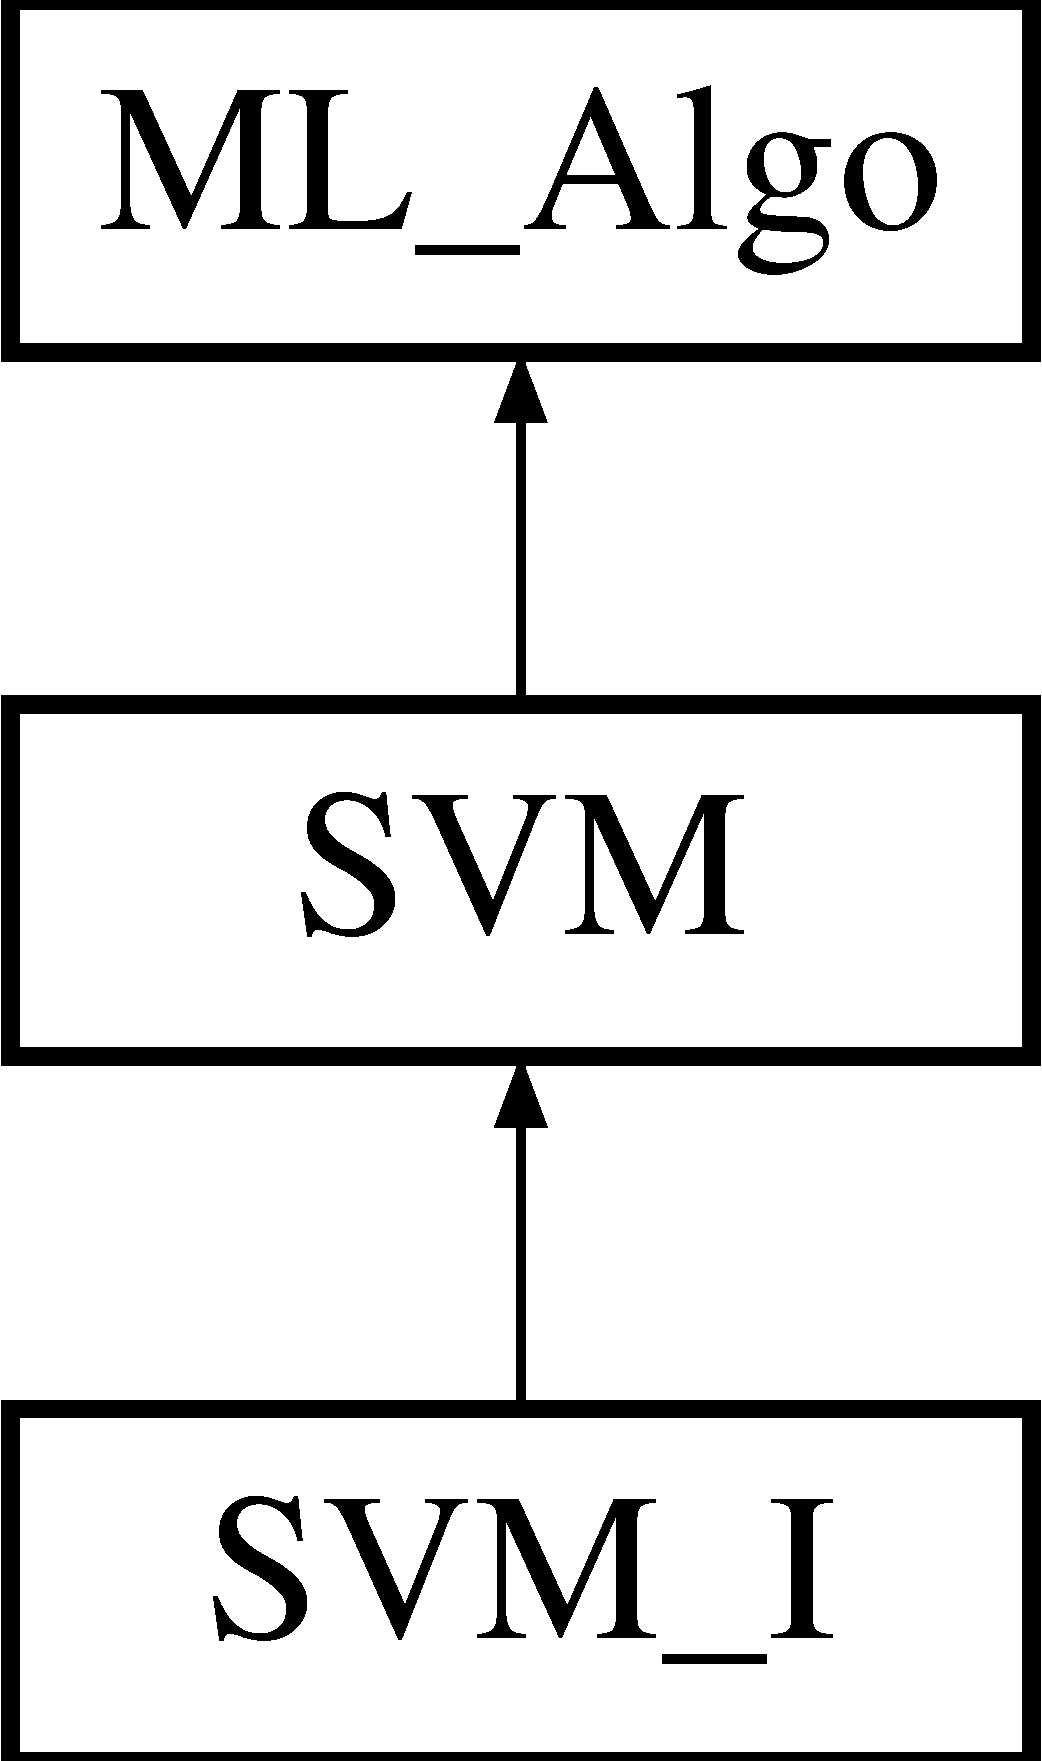
\includegraphics[height=3.000000cm]{classSVM__I}
\end{center}
\end{figure}
\subsection*{Public Member Functions}
\begin{DoxyCompactItemize}
\item 
\hyperlink{classSVM__I_aa7843beb94a2df684a5c8874322341c2}{S\+V\+M\+\_\+I} (void($\ast$f)(const char $\ast$)=N\+U\+LL, int \hyperlink{classSVM__I_a1b66cefe313cffaa77d4271dfb4b8474}{size}=10000, int equ=16)
\item 
\hyperlink{classSVM__I_a72cef53f36557c007f36a03724a62fb8}{$\sim$\+S\+V\+M\+\_\+I} ()
\item 
virtual int \hyperlink{classSVM__I_ab0236699daa4967cfec71234faa785c5}{prepare\+\_\+training\+\_\+data} (\hyperlink{classStates}{States} $\ast$gsets, int \&pre\+\_\+positive\+\_\+size, int \&pre\+\_\+negative\+\_\+size)
\item 
int \hyperlink{classSVM__I_abf732821c264b2cb8bef5d252991f2b6}{train} ()
\item 
double \hyperlink{classSVM__I_a643c2a6e58f8e70ab276ade9b1873bf6}{predict\+\_\+on\+\_\+training\+\_\+set} ()
\item 
virtual int \hyperlink{classSVM__I_a84470dce77add6377454c4408c6c1466}{check\+\_\+question\+\_\+set} (\hyperlink{classStates}{States} \&qset)
\item 
virtual int \hyperlink{classSVM__I_a5d1a8c93d41597aea5f31689687dbc77}{get\+\_\+converged} (\hyperlink{classEquation}{Equation} $\ast$, int)
\item 
virtual std\+::ostream \& \hyperlink{classSVM__I_ab0ae30d86d9f9026908a7b902f7a78e3}{\+\_\+print} (std\+::ostream \&out) const 
\item 
int \hyperlink{classSVM__I_a1b66cefe313cffaa77d4271dfb4b8474}{size} ()
\item 
virtual \hyperlink{classEquation}{Equation} $\ast$ \hyperlink{classSVM__I_a91b713ef0810fd4c83a5c711aea9fecf}{roundoff} (int \&num)
\item 
virtual int \hyperlink{classSVM__I_abe0a76aa6d31d18c2ee66002c35c813f}{predict} (double $\ast$v, int label=0)
\end{DoxyCompactItemize}
\subsection*{Data Fields}
\begin{DoxyCompactItemize}
\item 
\hyperlink{structsvm__model}{svm\+\_\+model} $\ast$ \hyperlink{classSVM__I_a7b7466c2246c73438ead77631278ff3a}{model}
\item 
\hyperlink{classEquation}{Equation} $\ast$ \hyperlink{classSVM__I_af905b6378094007502fa5d81f018a11b}{equations}
\item 
int \hyperlink{classSVM__I_ab674468eec42010761332da3f9b2f69c}{equ\+\_\+num}
\item 
\hyperlink{structsvm__parameter}{svm\+\_\+parameter} \hyperlink{classSVM__I_afbec56807dada05e9e527587d25acfb6}{param}
\item 
\hyperlink{classStates}{States} $\ast$ \hyperlink{classSVM__I_a8a56898f346ff15c5bb904ff6e001dad}{negatives}
\end{DoxyCompactItemize}
\subsection*{Protected Attributes}
\begin{DoxyCompactItemize}
\item 
int \hyperlink{classSVM__I_aaa890d6eaac46a447820a368f056eea7}{max\+\_\+equ}
\end{DoxyCompactItemize}
\subsection*{Private Member Functions}
\begin{DoxyCompactItemize}
\item 
double \hyperlink{classSVM__I_aa8eb2219340d322c9293e0d24a8b0e2e}{check\+\_\+postives\+\_\+and\+\_\+one\+\_\+negative} ()
\item 
int \hyperlink{classSVM__I_a099369c15005eea9f7d69c820431e0cb}{get\+\_\+misclassified} (int \&idx)
\end{DoxyCompactItemize}
\subsection*{Friends}
\begin{DoxyCompactItemize}
\item 
std\+::ostream \& \hyperlink{classSVM__I_ac0ce6164082022082361d78ba7b1c245}{operator$<$$<$} (std\+::ostream \&out, const \hyperlink{classSVM__I}{S\+V\+M\+\_\+I} \&svm\+\_\+i)
\end{DoxyCompactItemize}


\subsection{Constructor \& Destructor Documentation}
\index{S\+V\+M\+\_\+I@{S\+V\+M\+\_\+I}!S\+V\+M\+\_\+I@{S\+V\+M\+\_\+I}}
\index{S\+V\+M\+\_\+I@{S\+V\+M\+\_\+I}!S\+V\+M\+\_\+I@{S\+V\+M\+\_\+I}}
\subsubsection[{S\+V\+M\+\_\+\+I(void($\ast$f)(const char $\ast$)=\+N\+U\+L\+L, int size=10000, int equ=16)}]{\setlength{\rightskip}{0pt plus 5cm}S\+V\+M\+\_\+\+I\+::\+S\+V\+M\+\_\+I (
\begin{DoxyParamCaption}
\item[{void($\ast$)(const char $\ast$)}]{f = {\ttfamily NULL}, }
\item[{int}]{size = {\ttfamily 10000}, }
\item[{int}]{equ = {\ttfamily 16}}
\end{DoxyParamCaption}
)}\hypertarget{classSVM__I_aa7843beb94a2df684a5c8874322341c2}{}\label{classSVM__I_aa7843beb94a2df684a5c8874322341c2}
\index{S\+V\+M\+\_\+I@{S\+V\+M\+\_\+I}!````~S\+V\+M\+\_\+I@{$\sim$\+S\+V\+M\+\_\+I}}
\index{````~S\+V\+M\+\_\+I@{$\sim$\+S\+V\+M\+\_\+I}!S\+V\+M\+\_\+I@{S\+V\+M\+\_\+I}}
\subsubsection[{$\sim$\+S\+V\+M\+\_\+\+I()}]{\setlength{\rightskip}{0pt plus 5cm}S\+V\+M\+\_\+\+I\+::$\sim$\+S\+V\+M\+\_\+I (
\begin{DoxyParamCaption}
{}
\end{DoxyParamCaption}
)}\hypertarget{classSVM__I_a72cef53f36557c007f36a03724a62fb8}{}\label{classSVM__I_a72cef53f36557c007f36a03724a62fb8}


\subsection{Member Function Documentation}
\index{S\+V\+M\+\_\+I@{S\+V\+M\+\_\+I}!\+\_\+print@{\+\_\+print}}
\index{\+\_\+print@{\+\_\+print}!S\+V\+M\+\_\+I@{S\+V\+M\+\_\+I}}
\subsubsection[{\+\_\+print(std\+::ostream \&out) const }]{\setlength{\rightskip}{0pt plus 5cm}std\+::ostream \& S\+V\+M\+\_\+\+I\+::\+\_\+print (
\begin{DoxyParamCaption}
\item[{std\+::ostream \&}]{out}
\end{DoxyParamCaption}
) const\hspace{0.3cm}{\ttfamily [virtual]}}\hypertarget{classSVM__I_ab0ae30d86d9f9026908a7b902f7a78e3}{}\label{classSVM__I_ab0ae30d86d9f9026908a7b902f7a78e3}


Reimplemented from \hyperlink{classSVM_a6e5a3fbae4da1ecd4773173a2b590c21}{S\+VM}.

\index{S\+V\+M\+\_\+I@{S\+V\+M\+\_\+I}!check\+\_\+postives\+\_\+and\+\_\+one\+\_\+negative@{check\+\_\+postives\+\_\+and\+\_\+one\+\_\+negative}}
\index{check\+\_\+postives\+\_\+and\+\_\+one\+\_\+negative@{check\+\_\+postives\+\_\+and\+\_\+one\+\_\+negative}!S\+V\+M\+\_\+I@{S\+V\+M\+\_\+I}}
\subsubsection[{check\+\_\+postives\+\_\+and\+\_\+one\+\_\+negative()}]{\setlength{\rightskip}{0pt plus 5cm}double S\+V\+M\+\_\+\+I\+::check\+\_\+postives\+\_\+and\+\_\+one\+\_\+negative (
\begin{DoxyParamCaption}
{}
\end{DoxyParamCaption}
)\hspace{0.3cm}{\ttfamily [private]}}\hypertarget{classSVM__I_aa8eb2219340d322c9293e0d24a8b0e2e}{}\label{classSVM__I_aa8eb2219340d322c9293e0d24a8b0e2e}
\index{S\+V\+M\+\_\+I@{S\+V\+M\+\_\+I}!check\+\_\+question\+\_\+set@{check\+\_\+question\+\_\+set}}
\index{check\+\_\+question\+\_\+set@{check\+\_\+question\+\_\+set}!S\+V\+M\+\_\+I@{S\+V\+M\+\_\+I}}
\subsubsection[{check\+\_\+question\+\_\+set(\+States \&qset)}]{\setlength{\rightskip}{0pt plus 5cm}int S\+V\+M\+\_\+\+I\+::check\+\_\+question\+\_\+set (
\begin{DoxyParamCaption}
\item[{{\bf States} \&}]{qset}
\end{DoxyParamCaption}
)\hspace{0.3cm}{\ttfamily [virtual]}}\hypertarget{classSVM__I_a84470dce77add6377454c4408c6c1466}{}\label{classSVM__I_a84470dce77add6377454c4408c6c1466}


Reimplemented from \hyperlink{classSVM_aa610ec08173c8603ad6e02f26cbe8e1c}{S\+VM}.

\index{S\+V\+M\+\_\+I@{S\+V\+M\+\_\+I}!get\+\_\+converged@{get\+\_\+converged}}
\index{get\+\_\+converged@{get\+\_\+converged}!S\+V\+M\+\_\+I@{S\+V\+M\+\_\+I}}
\subsubsection[{get\+\_\+converged(\+Equation $\ast$, int)}]{\setlength{\rightskip}{0pt plus 5cm}int S\+V\+M\+\_\+\+I\+::get\+\_\+converged (
\begin{DoxyParamCaption}
\item[{{\bf Equation} $\ast$}]{previous\+\_\+equations, }
\item[{int}]{previous\+\_\+equation\+\_\+num}
\end{DoxyParamCaption}
)\hspace{0.3cm}{\ttfamily [virtual]}}\hypertarget{classSVM__I_a5d1a8c93d41597aea5f31689687dbc77}{}\label{classSVM__I_a5d1a8c93d41597aea5f31689687dbc77}


Reimplemented from \hyperlink{classSVM_a712dcd7cb65a8045a77dd474869dd5c4}{S\+VM}.

\index{S\+V\+M\+\_\+I@{S\+V\+M\+\_\+I}!get\+\_\+misclassified@{get\+\_\+misclassified}}
\index{get\+\_\+misclassified@{get\+\_\+misclassified}!S\+V\+M\+\_\+I@{S\+V\+M\+\_\+I}}
\subsubsection[{get\+\_\+misclassified(int \&idx)}]{\setlength{\rightskip}{0pt plus 5cm}int S\+V\+M\+\_\+\+I\+::get\+\_\+misclassified (
\begin{DoxyParamCaption}
\item[{int \&}]{idx}
\end{DoxyParamCaption}
)\hspace{0.3cm}{\ttfamily [private]}}\hypertarget{classSVM__I_a099369c15005eea9f7d69c820431e0cb}{}\label{classSVM__I_a099369c15005eea9f7d69c820431e0cb}
\index{S\+V\+M\+\_\+I@{S\+V\+M\+\_\+I}!predict@{predict}}
\index{predict@{predict}!S\+V\+M\+\_\+I@{S\+V\+M\+\_\+I}}
\subsubsection[{predict(double $\ast$v, int label=0)}]{\setlength{\rightskip}{0pt plus 5cm}int S\+V\+M\+\_\+\+I\+::predict (
\begin{DoxyParamCaption}
\item[{double $\ast$}]{v, }
\item[{int}]{label = {\ttfamily 0}}
\end{DoxyParamCaption}
)\hspace{0.3cm}{\ttfamily [virtual]}}\hypertarget{classSVM__I_abe0a76aa6d31d18c2ee66002c35c813f}{}\label{classSVM__I_abe0a76aa6d31d18c2ee66002c35c813f}


Reimplemented from \hyperlink{classSVM_a972215d3c749ba550c85763c8871567f}{S\+VM}.

\index{S\+V\+M\+\_\+I@{S\+V\+M\+\_\+I}!predict\+\_\+on\+\_\+training\+\_\+set@{predict\+\_\+on\+\_\+training\+\_\+set}}
\index{predict\+\_\+on\+\_\+training\+\_\+set@{predict\+\_\+on\+\_\+training\+\_\+set}!S\+V\+M\+\_\+I@{S\+V\+M\+\_\+I}}
\subsubsection[{predict\+\_\+on\+\_\+training\+\_\+set()}]{\setlength{\rightskip}{0pt plus 5cm}double S\+V\+M\+\_\+\+I\+::predict\+\_\+on\+\_\+training\+\_\+set (
\begin{DoxyParamCaption}
{}
\end{DoxyParamCaption}
)\hspace{0.3cm}{\ttfamily [virtual]}}\hypertarget{classSVM__I_a643c2a6e58f8e70ab276ade9b1873bf6}{}\label{classSVM__I_a643c2a6e58f8e70ab276ade9b1873bf6}


Reimplemented from \hyperlink{classSVM_af208fc653a382591f20c0fcf7a186362}{S\+VM}.

\index{S\+V\+M\+\_\+I@{S\+V\+M\+\_\+I}!prepare\+\_\+training\+\_\+data@{prepare\+\_\+training\+\_\+data}}
\index{prepare\+\_\+training\+\_\+data@{prepare\+\_\+training\+\_\+data}!S\+V\+M\+\_\+I@{S\+V\+M\+\_\+I}}
\subsubsection[{prepare\+\_\+training\+\_\+data(\+States $\ast$gsets, int \&pre\+\_\+positive\+\_\+size, int \&pre\+\_\+negative\+\_\+size)}]{\setlength{\rightskip}{0pt plus 5cm}int S\+V\+M\+\_\+\+I\+::prepare\+\_\+training\+\_\+data (
\begin{DoxyParamCaption}
\item[{{\bf States} $\ast$}]{gsets, }
\item[{int \&}]{pre\+\_\+positive\+\_\+size, }
\item[{int \&}]{pre\+\_\+negative\+\_\+size}
\end{DoxyParamCaption}
)\hspace{0.3cm}{\ttfamily [virtual]}}\hypertarget{classSVM__I_ab0236699daa4967cfec71234faa785c5}{}\label{classSVM__I_ab0236699daa4967cfec71234faa785c5}


Reimplemented from \hyperlink{classSVM_a930fe217e3affd64acb6700f5f8082e1}{S\+VM}.

\index{S\+V\+M\+\_\+I@{S\+V\+M\+\_\+I}!roundoff@{roundoff}}
\index{roundoff@{roundoff}!S\+V\+M\+\_\+I@{S\+V\+M\+\_\+I}}
\subsubsection[{roundoff(int \&num)}]{\setlength{\rightskip}{0pt plus 5cm}{\bf Equation} $\ast$ S\+V\+M\+\_\+\+I\+::roundoff (
\begin{DoxyParamCaption}
\item[{int \&}]{num}
\end{DoxyParamCaption}
)\hspace{0.3cm}{\ttfamily [virtual]}}\hypertarget{classSVM__I_a91b713ef0810fd4c83a5c711aea9fecf}{}\label{classSVM__I_a91b713ef0810fd4c83a5c711aea9fecf}


Reimplemented from \hyperlink{classSVM_abd2d511c6cb9f64a29a4551f6435bfd2}{S\+VM}.

\index{S\+V\+M\+\_\+I@{S\+V\+M\+\_\+I}!size@{size}}
\index{size@{size}!S\+V\+M\+\_\+I@{S\+V\+M\+\_\+I}}
\subsubsection[{size()}]{\setlength{\rightskip}{0pt plus 5cm}int S\+V\+M\+\_\+\+I\+::size (
\begin{DoxyParamCaption}
{}
\end{DoxyParamCaption}
)\hspace{0.3cm}{\ttfamily [virtual]}}\hypertarget{classSVM__I_a1b66cefe313cffaa77d4271dfb4b8474}{}\label{classSVM__I_a1b66cefe313cffaa77d4271dfb4b8474}


Reimplemented from \hyperlink{classSVM_a4563cef982f6e1c67acf0c7b0ec8909b}{S\+VM}.

\index{S\+V\+M\+\_\+I@{S\+V\+M\+\_\+I}!train@{train}}
\index{train@{train}!S\+V\+M\+\_\+I@{S\+V\+M\+\_\+I}}
\subsubsection[{train()}]{\setlength{\rightskip}{0pt plus 5cm}int S\+V\+M\+\_\+\+I\+::train (
\begin{DoxyParamCaption}
{}
\end{DoxyParamCaption}
)\hspace{0.3cm}{\ttfamily [virtual]}}\hypertarget{classSVM__I_abf732821c264b2cb8bef5d252991f2b6}{}\label{classSVM__I_abf732821c264b2cb8bef5d252991f2b6}


Reimplemented from \hyperlink{classSVM_a6a1d895b86522eab683d66ded4d3a049}{S\+VM}.



\subsection{Friends And Related Function Documentation}
\index{S\+V\+M\+\_\+I@{S\+V\+M\+\_\+I}!operator$<$$<$@{operator$<$$<$}}
\index{operator$<$$<$@{operator$<$$<$}!S\+V\+M\+\_\+I@{S\+V\+M\+\_\+I}}
\subsubsection[{operator$<$$<$}]{\setlength{\rightskip}{0pt plus 5cm}std\+::ostream\& operator$<$$<$ (
\begin{DoxyParamCaption}
\item[{std\+::ostream \&}]{out, }
\item[{const {\bf S\+V\+M\+\_\+I} \&}]{svm\+\_\+i}
\end{DoxyParamCaption}
)\hspace{0.3cm}{\ttfamily [friend]}}\hypertarget{classSVM__I_ac0ce6164082022082361d78ba7b1c245}{}\label{classSVM__I_ac0ce6164082022082361d78ba7b1c245}


\subsection{Field Documentation}
\index{S\+V\+M\+\_\+I@{S\+V\+M\+\_\+I}!equ\+\_\+num@{equ\+\_\+num}}
\index{equ\+\_\+num@{equ\+\_\+num}!S\+V\+M\+\_\+I@{S\+V\+M\+\_\+I}}
\subsubsection[{equ\+\_\+num}]{\setlength{\rightskip}{0pt plus 5cm}int S\+V\+M\+\_\+\+I\+::equ\+\_\+num}\hypertarget{classSVM__I_ab674468eec42010761332da3f9b2f69c}{}\label{classSVM__I_ab674468eec42010761332da3f9b2f69c}
\index{S\+V\+M\+\_\+I@{S\+V\+M\+\_\+I}!equations@{equations}}
\index{equations@{equations}!S\+V\+M\+\_\+I@{S\+V\+M\+\_\+I}}
\subsubsection[{equations}]{\setlength{\rightskip}{0pt plus 5cm}{\bf Equation}$\ast$ S\+V\+M\+\_\+\+I\+::equations}\hypertarget{classSVM__I_af905b6378094007502fa5d81f018a11b}{}\label{classSVM__I_af905b6378094007502fa5d81f018a11b}
\index{S\+V\+M\+\_\+I@{S\+V\+M\+\_\+I}!max\+\_\+equ@{max\+\_\+equ}}
\index{max\+\_\+equ@{max\+\_\+equ}!S\+V\+M\+\_\+I@{S\+V\+M\+\_\+I}}
\subsubsection[{max\+\_\+equ}]{\setlength{\rightskip}{0pt plus 5cm}int S\+V\+M\+\_\+\+I\+::max\+\_\+equ\hspace{0.3cm}{\ttfamily [protected]}}\hypertarget{classSVM__I_aaa890d6eaac46a447820a368f056eea7}{}\label{classSVM__I_aaa890d6eaac46a447820a368f056eea7}
\index{S\+V\+M\+\_\+I@{S\+V\+M\+\_\+I}!model@{model}}
\index{model@{model}!S\+V\+M\+\_\+I@{S\+V\+M\+\_\+I}}
\subsubsection[{model}]{\setlength{\rightskip}{0pt plus 5cm}{\bf svm\+\_\+model}$\ast$ S\+V\+M\+\_\+\+I\+::model}\hypertarget{classSVM__I_a7b7466c2246c73438ead77631278ff3a}{}\label{classSVM__I_a7b7466c2246c73438ead77631278ff3a}
\index{S\+V\+M\+\_\+I@{S\+V\+M\+\_\+I}!negatives@{negatives}}
\index{negatives@{negatives}!S\+V\+M\+\_\+I@{S\+V\+M\+\_\+I}}
\subsubsection[{negatives}]{\setlength{\rightskip}{0pt plus 5cm}{\bf States}$\ast$ S\+V\+M\+\_\+\+I\+::negatives}\hypertarget{classSVM__I_a8a56898f346ff15c5bb904ff6e001dad}{}\label{classSVM__I_a8a56898f346ff15c5bb904ff6e001dad}
\index{S\+V\+M\+\_\+I@{S\+V\+M\+\_\+I}!param@{param}}
\index{param@{param}!S\+V\+M\+\_\+I@{S\+V\+M\+\_\+I}}
\subsubsection[{param}]{\setlength{\rightskip}{0pt plus 5cm}{\bf svm\+\_\+parameter} S\+V\+M\+\_\+\+I\+::param}\hypertarget{classSVM__I_afbec56807dada05e9e527587d25acfb6}{}\label{classSVM__I_afbec56807dada05e9e527587d25acfb6}


The documentation for this class was generated from the following files\+:\begin{DoxyCompactItemize}
\item 
include/\hyperlink{svm__i_8h}{svm\+\_\+i.\+h}\item 
src/\hyperlink{svm__i_8cpp}{svm\+\_\+i.\+cpp}\end{DoxyCompactItemize}

\hypertarget{structsvm__model}{}\section{svm\+\_\+model Struct Reference}
\label{structsvm__model}\index{svm\+\_\+model@{svm\+\_\+model}}


{\ttfamily \#include $<$svm\+\_\+core.\+h$>$}

\subsection*{Data Fields}
\begin{DoxyCompactItemize}
\item 
struct \hyperlink{structsvm__parameter}{svm\+\_\+parameter} \hyperlink{structsvm__model_a95f43f398a173e63d0ce26911d0a9273}{param}
\item 
int \hyperlink{structsvm__model_a5af6e0cfb063e8aac03c99aa9d319116}{nr\+\_\+class}
\item 
int \hyperlink{structsvm__model_ab858d7eed0bd3cc4c33c094872643d0a}{l}
\item 
struct \hyperlink{structsvm__node}{svm\+\_\+node} $\ast$$\ast$ \hyperlink{structsvm__model_a96da6fe173a7150dae95bf55d5539e45}{SV}
\item 
double $\ast$$\ast$ \hyperlink{structsvm__model_a978084d722ac886100ffcc35fc931143}{sv\+\_\+coef}
\item 
double $\ast$ \hyperlink{structsvm__model_a16e4dea1508f93ece4384ec35c991887}{rho}
\item 
double $\ast$ \hyperlink{structsvm__model_adf5f28fcdd3ca1c5b23c1f6167710a04}{probA}
\item 
double $\ast$ \hyperlink{structsvm__model_a73ba8feaaf3c2c38c6bb81f7bcb5809e}{probB}
\item 
int $\ast$ \hyperlink{structsvm__model_add7f649bf78428c38a282ed8776fa433}{sv\+\_\+indices}
\item 
int $\ast$ \hyperlink{structsvm__model_ac66d192809e92b95875bdf8ebb749060}{label}
\item 
int $\ast$ \hyperlink{structsvm__model_a1d342c9b9e5e4a6377862e13123a25ef}{n\+SV}
\item 
int \hyperlink{structsvm__model_a2ae57ce1fa43497d151aff26c21a13a1}{free\+\_\+sv}
\end{DoxyCompactItemize}


\subsection{Field Documentation}
\index{svm\+\_\+model@{svm\+\_\+model}!free\+\_\+sv@{free\+\_\+sv}}
\index{free\+\_\+sv@{free\+\_\+sv}!svm\+\_\+model@{svm\+\_\+model}}
\subsubsection[{free\+\_\+sv}]{\setlength{\rightskip}{0pt plus 5cm}int svm\+\_\+model\+::free\+\_\+sv}\hypertarget{structsvm__model_a2ae57ce1fa43497d151aff26c21a13a1}{}\label{structsvm__model_a2ae57ce1fa43497d151aff26c21a13a1}
\index{svm\+\_\+model@{svm\+\_\+model}!l@{l}}
\index{l@{l}!svm\+\_\+model@{svm\+\_\+model}}
\subsubsection[{l}]{\setlength{\rightskip}{0pt plus 5cm}int svm\+\_\+model\+::l}\hypertarget{structsvm__model_ab858d7eed0bd3cc4c33c094872643d0a}{}\label{structsvm__model_ab858d7eed0bd3cc4c33c094872643d0a}
\index{svm\+\_\+model@{svm\+\_\+model}!label@{label}}
\index{label@{label}!svm\+\_\+model@{svm\+\_\+model}}
\subsubsection[{label}]{\setlength{\rightskip}{0pt plus 5cm}int$\ast$ svm\+\_\+model\+::label}\hypertarget{structsvm__model_ac66d192809e92b95875bdf8ebb749060}{}\label{structsvm__model_ac66d192809e92b95875bdf8ebb749060}
\index{svm\+\_\+model@{svm\+\_\+model}!nr\+\_\+class@{nr\+\_\+class}}
\index{nr\+\_\+class@{nr\+\_\+class}!svm\+\_\+model@{svm\+\_\+model}}
\subsubsection[{nr\+\_\+class}]{\setlength{\rightskip}{0pt plus 5cm}int svm\+\_\+model\+::nr\+\_\+class}\hypertarget{structsvm__model_a5af6e0cfb063e8aac03c99aa9d319116}{}\label{structsvm__model_a5af6e0cfb063e8aac03c99aa9d319116}
\index{svm\+\_\+model@{svm\+\_\+model}!n\+SV@{n\+SV}}
\index{n\+SV@{n\+SV}!svm\+\_\+model@{svm\+\_\+model}}
\subsubsection[{n\+SV}]{\setlength{\rightskip}{0pt plus 5cm}int$\ast$ svm\+\_\+model\+::n\+SV}\hypertarget{structsvm__model_a1d342c9b9e5e4a6377862e13123a25ef}{}\label{structsvm__model_a1d342c9b9e5e4a6377862e13123a25ef}
\index{svm\+\_\+model@{svm\+\_\+model}!param@{param}}
\index{param@{param}!svm\+\_\+model@{svm\+\_\+model}}
\subsubsection[{param}]{\setlength{\rightskip}{0pt plus 5cm}struct {\bf svm\+\_\+parameter} svm\+\_\+model\+::param}\hypertarget{structsvm__model_a95f43f398a173e63d0ce26911d0a9273}{}\label{structsvm__model_a95f43f398a173e63d0ce26911d0a9273}
\index{svm\+\_\+model@{svm\+\_\+model}!probA@{probA}}
\index{probA@{probA}!svm\+\_\+model@{svm\+\_\+model}}
\subsubsection[{probA}]{\setlength{\rightskip}{0pt plus 5cm}double$\ast$ svm\+\_\+model\+::probA}\hypertarget{structsvm__model_adf5f28fcdd3ca1c5b23c1f6167710a04}{}\label{structsvm__model_adf5f28fcdd3ca1c5b23c1f6167710a04}
\index{svm\+\_\+model@{svm\+\_\+model}!probB@{probB}}
\index{probB@{probB}!svm\+\_\+model@{svm\+\_\+model}}
\subsubsection[{probB}]{\setlength{\rightskip}{0pt plus 5cm}double$\ast$ svm\+\_\+model\+::probB}\hypertarget{structsvm__model_a73ba8feaaf3c2c38c6bb81f7bcb5809e}{}\label{structsvm__model_a73ba8feaaf3c2c38c6bb81f7bcb5809e}
\index{svm\+\_\+model@{svm\+\_\+model}!rho@{rho}}
\index{rho@{rho}!svm\+\_\+model@{svm\+\_\+model}}
\subsubsection[{rho}]{\setlength{\rightskip}{0pt plus 5cm}double$\ast$ svm\+\_\+model\+::rho}\hypertarget{structsvm__model_a16e4dea1508f93ece4384ec35c991887}{}\label{structsvm__model_a16e4dea1508f93ece4384ec35c991887}
\index{svm\+\_\+model@{svm\+\_\+model}!SV@{SV}}
\index{SV@{SV}!svm\+\_\+model@{svm\+\_\+model}}
\subsubsection[{SV}]{\setlength{\rightskip}{0pt plus 5cm}struct {\bf svm\+\_\+node}$\ast$$\ast$ svm\+\_\+model\+::\+SV}\hypertarget{structsvm__model_a96da6fe173a7150dae95bf55d5539e45}{}\label{structsvm__model_a96da6fe173a7150dae95bf55d5539e45}
\index{svm\+\_\+model@{svm\+\_\+model}!sv\+\_\+coef@{sv\+\_\+coef}}
\index{sv\+\_\+coef@{sv\+\_\+coef}!svm\+\_\+model@{svm\+\_\+model}}
\subsubsection[{sv\+\_\+coef}]{\setlength{\rightskip}{0pt plus 5cm}double$\ast$$\ast$ svm\+\_\+model\+::sv\+\_\+coef}\hypertarget{structsvm__model_a978084d722ac886100ffcc35fc931143}{}\label{structsvm__model_a978084d722ac886100ffcc35fc931143}
\index{svm\+\_\+model@{svm\+\_\+model}!sv\+\_\+indices@{sv\+\_\+indices}}
\index{sv\+\_\+indices@{sv\+\_\+indices}!svm\+\_\+model@{svm\+\_\+model}}
\subsubsection[{sv\+\_\+indices}]{\setlength{\rightskip}{0pt plus 5cm}int$\ast$ svm\+\_\+model\+::sv\+\_\+indices}\hypertarget{structsvm__model_add7f649bf78428c38a282ed8776fa433}{}\label{structsvm__model_add7f649bf78428c38a282ed8776fa433}


The documentation for this struct was generated from the following file\+:\begin{DoxyCompactItemize}
\item 
include/\hyperlink{svm__core_8h}{svm\+\_\+core.\+h}\end{DoxyCompactItemize}

\hypertarget{structsvm__node}{}\section{svm\+\_\+node Struct Reference}
\label{structsvm__node}\index{svm\+\_\+node@{svm\+\_\+node}}


{\ttfamily \#include $<$svm\+\_\+core.\+h$>$}

\subsection*{Data Fields}
\begin{DoxyCompactItemize}
\item 
double \hyperlink{structsvm__node_a9ca47b8a156238d04213453f3b89e177}{value}
\end{DoxyCompactItemize}
\subsection*{Friends}
\begin{DoxyCompactItemize}
\item 
std\+::ostream \& \hyperlink{structsvm__node_a851da78d2b442fd68042fa3b6debfc66}{operator$<$$<$} (std\+::ostream \&out, const \hyperlink{structsvm__node}{svm\+\_\+node} \&sn)
\end{DoxyCompactItemize}


\subsection{Friends And Related Function Documentation}
\index{svm\+\_\+node@{svm\+\_\+node}!operator$<$$<$@{operator$<$$<$}}
\index{operator$<$$<$@{operator$<$$<$}!svm\+\_\+node@{svm\+\_\+node}}
\subsubsection[{operator$<$$<$}]{\setlength{\rightskip}{0pt plus 5cm}std\+::ostream\& operator$<$$<$ (
\begin{DoxyParamCaption}
\item[{std\+::ostream \&}]{out, }
\item[{const {\bf svm\+\_\+node} \&}]{sn}
\end{DoxyParamCaption}
)\hspace{0.3cm}{\ttfamily [friend]}}\hypertarget{structsvm__node_a851da78d2b442fd68042fa3b6debfc66}{}\label{structsvm__node_a851da78d2b442fd68042fa3b6debfc66}


\subsection{Field Documentation}
\index{svm\+\_\+node@{svm\+\_\+node}!value@{value}}
\index{value@{value}!svm\+\_\+node@{svm\+\_\+node}}
\subsubsection[{value}]{\setlength{\rightskip}{0pt plus 5cm}double svm\+\_\+node\+::value}\hypertarget{structsvm__node_a9ca47b8a156238d04213453f3b89e177}{}\label{structsvm__node_a9ca47b8a156238d04213453f3b89e177}


The documentation for this struct was generated from the following file\+:\begin{DoxyCompactItemize}
\item 
include/\hyperlink{svm__core_8h}{svm\+\_\+core.\+h}\end{DoxyCompactItemize}

\hypertarget{structsvm__parameter}{}\section{svm\+\_\+parameter Struct Reference}
\label{structsvm__parameter}\index{svm\+\_\+parameter@{svm\+\_\+parameter}}


{\ttfamily \#include $<$svm\+\_\+core.\+h$>$}

\subsection*{Data Fields}
\begin{DoxyCompactItemize}
\item 
int \hyperlink{structsvm__parameter_a3afb37272180a903df05f7b649b338f4}{svm\+\_\+type}
\item 
int \hyperlink{structsvm__parameter_a4188713ba31fc3d101244a6bcc09a760}{kernel\+\_\+type}
\item 
int \hyperlink{structsvm__parameter_afef1c4508ec0045c236a3308b0fa5138}{degree}
\item 
double \hyperlink{structsvm__parameter_a91667b90506e171482b5fc619377110d}{gamma}
\item 
double \hyperlink{structsvm__parameter_a3ab3555a96a578bea6e5285a5db0a4db}{coef0}
\item 
double \hyperlink{structsvm__parameter_a00286b7e0767e45d68ac7abceb60c821}{cache\+\_\+size}
\item 
double \hyperlink{structsvm__parameter_a1feab5a4e0d5842a20e544f3f944f841}{eps}
\item 
double \hyperlink{structsvm__parameter_af4f905a3f7d589d86964289af3c9d812}{C}
\item 
int \hyperlink{structsvm__parameter_a44014738d1db5444f7f9a1ebf74e4214}{nr\+\_\+weight}
\item 
int $\ast$ \hyperlink{structsvm__parameter_a06753922bb0282240f35ae7683f8d69a}{weight\+\_\+label}
\item 
double $\ast$ \hyperlink{structsvm__parameter_afff750f99180b5ddf735404496b6c196}{weight}
\item 
double \hyperlink{structsvm__parameter_a4c20c566cb61d5808e8cabd7adbc35c1}{nu}
\item 
double \hyperlink{structsvm__parameter_a3b60d7ce96137a64caca81095d1a188b}{p}
\item 
int \hyperlink{structsvm__parameter_afdbccdf6a24be650d75804b783edc347}{shrinking}
\item 
int \hyperlink{structsvm__parameter_afac0ef02879d7e27e17ac2a75115a7d9}{probability}
\end{DoxyCompactItemize}


\subsection{Field Documentation}
\index{svm\+\_\+parameter@{svm\+\_\+parameter}!C@{C}}
\index{C@{C}!svm\+\_\+parameter@{svm\+\_\+parameter}}
\subsubsection[{C}]{\setlength{\rightskip}{0pt plus 5cm}double svm\+\_\+parameter\+::C}\hypertarget{structsvm__parameter_af4f905a3f7d589d86964289af3c9d812}{}\label{structsvm__parameter_af4f905a3f7d589d86964289af3c9d812}
\index{svm\+\_\+parameter@{svm\+\_\+parameter}!cache\+\_\+size@{cache\+\_\+size}}
\index{cache\+\_\+size@{cache\+\_\+size}!svm\+\_\+parameter@{svm\+\_\+parameter}}
\subsubsection[{cache\+\_\+size}]{\setlength{\rightskip}{0pt plus 5cm}double svm\+\_\+parameter\+::cache\+\_\+size}\hypertarget{structsvm__parameter_a00286b7e0767e45d68ac7abceb60c821}{}\label{structsvm__parameter_a00286b7e0767e45d68ac7abceb60c821}
\index{svm\+\_\+parameter@{svm\+\_\+parameter}!coef0@{coef0}}
\index{coef0@{coef0}!svm\+\_\+parameter@{svm\+\_\+parameter}}
\subsubsection[{coef0}]{\setlength{\rightskip}{0pt plus 5cm}double svm\+\_\+parameter\+::coef0}\hypertarget{structsvm__parameter_a3ab3555a96a578bea6e5285a5db0a4db}{}\label{structsvm__parameter_a3ab3555a96a578bea6e5285a5db0a4db}
\index{svm\+\_\+parameter@{svm\+\_\+parameter}!degree@{degree}}
\index{degree@{degree}!svm\+\_\+parameter@{svm\+\_\+parameter}}
\subsubsection[{degree}]{\setlength{\rightskip}{0pt plus 5cm}int svm\+\_\+parameter\+::degree}\hypertarget{structsvm__parameter_afef1c4508ec0045c236a3308b0fa5138}{}\label{structsvm__parameter_afef1c4508ec0045c236a3308b0fa5138}
\index{svm\+\_\+parameter@{svm\+\_\+parameter}!eps@{eps}}
\index{eps@{eps}!svm\+\_\+parameter@{svm\+\_\+parameter}}
\subsubsection[{eps}]{\setlength{\rightskip}{0pt plus 5cm}double svm\+\_\+parameter\+::eps}\hypertarget{structsvm__parameter_a1feab5a4e0d5842a20e544f3f944f841}{}\label{structsvm__parameter_a1feab5a4e0d5842a20e544f3f944f841}
\index{svm\+\_\+parameter@{svm\+\_\+parameter}!gamma@{gamma}}
\index{gamma@{gamma}!svm\+\_\+parameter@{svm\+\_\+parameter}}
\subsubsection[{gamma}]{\setlength{\rightskip}{0pt plus 5cm}double svm\+\_\+parameter\+::gamma}\hypertarget{structsvm__parameter_a91667b90506e171482b5fc619377110d}{}\label{structsvm__parameter_a91667b90506e171482b5fc619377110d}
\index{svm\+\_\+parameter@{svm\+\_\+parameter}!kernel\+\_\+type@{kernel\+\_\+type}}
\index{kernel\+\_\+type@{kernel\+\_\+type}!svm\+\_\+parameter@{svm\+\_\+parameter}}
\subsubsection[{kernel\+\_\+type}]{\setlength{\rightskip}{0pt plus 5cm}int svm\+\_\+parameter\+::kernel\+\_\+type}\hypertarget{structsvm__parameter_a4188713ba31fc3d101244a6bcc09a760}{}\label{structsvm__parameter_a4188713ba31fc3d101244a6bcc09a760}
\index{svm\+\_\+parameter@{svm\+\_\+parameter}!nr\+\_\+weight@{nr\+\_\+weight}}
\index{nr\+\_\+weight@{nr\+\_\+weight}!svm\+\_\+parameter@{svm\+\_\+parameter}}
\subsubsection[{nr\+\_\+weight}]{\setlength{\rightskip}{0pt plus 5cm}int svm\+\_\+parameter\+::nr\+\_\+weight}\hypertarget{structsvm__parameter_a44014738d1db5444f7f9a1ebf74e4214}{}\label{structsvm__parameter_a44014738d1db5444f7f9a1ebf74e4214}
\index{svm\+\_\+parameter@{svm\+\_\+parameter}!nu@{nu}}
\index{nu@{nu}!svm\+\_\+parameter@{svm\+\_\+parameter}}
\subsubsection[{nu}]{\setlength{\rightskip}{0pt plus 5cm}double svm\+\_\+parameter\+::nu}\hypertarget{structsvm__parameter_a4c20c566cb61d5808e8cabd7adbc35c1}{}\label{structsvm__parameter_a4c20c566cb61d5808e8cabd7adbc35c1}
\index{svm\+\_\+parameter@{svm\+\_\+parameter}!p@{p}}
\index{p@{p}!svm\+\_\+parameter@{svm\+\_\+parameter}}
\subsubsection[{p}]{\setlength{\rightskip}{0pt plus 5cm}double svm\+\_\+parameter\+::p}\hypertarget{structsvm__parameter_a3b60d7ce96137a64caca81095d1a188b}{}\label{structsvm__parameter_a3b60d7ce96137a64caca81095d1a188b}
\index{svm\+\_\+parameter@{svm\+\_\+parameter}!probability@{probability}}
\index{probability@{probability}!svm\+\_\+parameter@{svm\+\_\+parameter}}
\subsubsection[{probability}]{\setlength{\rightskip}{0pt plus 5cm}int svm\+\_\+parameter\+::probability}\hypertarget{structsvm__parameter_afac0ef02879d7e27e17ac2a75115a7d9}{}\label{structsvm__parameter_afac0ef02879d7e27e17ac2a75115a7d9}
\index{svm\+\_\+parameter@{svm\+\_\+parameter}!shrinking@{shrinking}}
\index{shrinking@{shrinking}!svm\+\_\+parameter@{svm\+\_\+parameter}}
\subsubsection[{shrinking}]{\setlength{\rightskip}{0pt plus 5cm}int svm\+\_\+parameter\+::shrinking}\hypertarget{structsvm__parameter_afdbccdf6a24be650d75804b783edc347}{}\label{structsvm__parameter_afdbccdf6a24be650d75804b783edc347}
\index{svm\+\_\+parameter@{svm\+\_\+parameter}!svm\+\_\+type@{svm\+\_\+type}}
\index{svm\+\_\+type@{svm\+\_\+type}!svm\+\_\+parameter@{svm\+\_\+parameter}}
\subsubsection[{svm\+\_\+type}]{\setlength{\rightskip}{0pt plus 5cm}int svm\+\_\+parameter\+::svm\+\_\+type}\hypertarget{structsvm__parameter_a3afb37272180a903df05f7b649b338f4}{}\label{structsvm__parameter_a3afb37272180a903df05f7b649b338f4}
\index{svm\+\_\+parameter@{svm\+\_\+parameter}!weight@{weight}}
\index{weight@{weight}!svm\+\_\+parameter@{svm\+\_\+parameter}}
\subsubsection[{weight}]{\setlength{\rightskip}{0pt plus 5cm}double$\ast$ svm\+\_\+parameter\+::weight}\hypertarget{structsvm__parameter_afff750f99180b5ddf735404496b6c196}{}\label{structsvm__parameter_afff750f99180b5ddf735404496b6c196}
\index{svm\+\_\+parameter@{svm\+\_\+parameter}!weight\+\_\+label@{weight\+\_\+label}}
\index{weight\+\_\+label@{weight\+\_\+label}!svm\+\_\+parameter@{svm\+\_\+parameter}}
\subsubsection[{weight\+\_\+label}]{\setlength{\rightskip}{0pt plus 5cm}int$\ast$ svm\+\_\+parameter\+::weight\+\_\+label}\hypertarget{structsvm__parameter_a06753922bb0282240f35ae7683f8d69a}{}\label{structsvm__parameter_a06753922bb0282240f35ae7683f8d69a}


The documentation for this struct was generated from the following file\+:\begin{DoxyCompactItemize}
\item 
include/\hyperlink{svm__core_8h}{svm\+\_\+core.\+h}\end{DoxyCompactItemize}

\hypertarget{structsvm__problem}{}\section{svm\+\_\+problem Struct Reference}
\label{structsvm__problem}\index{svm\+\_\+problem@{svm\+\_\+problem}}


{\ttfamily \#include $<$svm\+\_\+core.\+h$>$}

\subsection*{Data Fields}
\begin{DoxyCompactItemize}
\item 
int \hyperlink{structsvm__problem_a4350eb6820f0d6126bffb6264cec65b3}{l}
\item 
double $\ast$ \hyperlink{structsvm__problem_a59dec12ff090571bc9592ba9fb306780}{y}
\item 
struct \hyperlink{structsvm__node}{svm\+\_\+node} $\ast$$\ast$ \hyperlink{structsvm__problem_acddda9b49a8e38bbda079f35c2e18984}{x}
\end{DoxyCompactItemize}
\subsection*{Friends}
\begin{DoxyCompactItemize}
\item 
std\+::ostream \& \hyperlink{structsvm__problem_af76b29900587df02955339129610ae53}{operator$<$$<$} (std\+::ostream \&out, const \hyperlink{structsvm__problem}{svm\+\_\+problem} \&sp)
\end{DoxyCompactItemize}


\subsection{Friends And Related Function Documentation}
\index{svm\+\_\+problem@{svm\+\_\+problem}!operator$<$$<$@{operator$<$$<$}}
\index{operator$<$$<$@{operator$<$$<$}!svm\+\_\+problem@{svm\+\_\+problem}}
\subsubsection[{operator$<$$<$}]{\setlength{\rightskip}{0pt plus 5cm}std\+::ostream\& operator$<$$<$ (
\begin{DoxyParamCaption}
\item[{std\+::ostream \&}]{out, }
\item[{const {\bf svm\+\_\+problem} \&}]{sp}
\end{DoxyParamCaption}
)\hspace{0.3cm}{\ttfamily [friend]}}\hypertarget{structsvm__problem_af76b29900587df02955339129610ae53}{}\label{structsvm__problem_af76b29900587df02955339129610ae53}


\subsection{Field Documentation}
\index{svm\+\_\+problem@{svm\+\_\+problem}!l@{l}}
\index{l@{l}!svm\+\_\+problem@{svm\+\_\+problem}}
\subsubsection[{l}]{\setlength{\rightskip}{0pt plus 5cm}int svm\+\_\+problem\+::l}\hypertarget{structsvm__problem_a4350eb6820f0d6126bffb6264cec65b3}{}\label{structsvm__problem_a4350eb6820f0d6126bffb6264cec65b3}
\index{svm\+\_\+problem@{svm\+\_\+problem}!x@{x}}
\index{x@{x}!svm\+\_\+problem@{svm\+\_\+problem}}
\subsubsection[{x}]{\setlength{\rightskip}{0pt plus 5cm}struct {\bf svm\+\_\+node}$\ast$$\ast$ svm\+\_\+problem\+::x}\hypertarget{structsvm__problem_acddda9b49a8e38bbda079f35c2e18984}{}\label{structsvm__problem_acddda9b49a8e38bbda079f35c2e18984}
\index{svm\+\_\+problem@{svm\+\_\+problem}!y@{y}}
\index{y@{y}!svm\+\_\+problem@{svm\+\_\+problem}}
\subsubsection[{y}]{\setlength{\rightskip}{0pt plus 5cm}double$\ast$ svm\+\_\+problem\+::y}\hypertarget{structsvm__problem_a59dec12ff090571bc9592ba9fb306780}{}\label{structsvm__problem_a59dec12ff090571bc9592ba9fb306780}


The documentation for this struct was generated from the following file\+:\begin{DoxyCompactItemize}
\item 
include/\hyperlink{svm__core_8h}{svm\+\_\+core.\+h}\end{DoxyCompactItemize}

\hypertarget{classSVR__Q}{}\section{S\+V\+R\+\_\+Q Class Reference}
\label{classSVR__Q}\index{S\+V\+R\+\_\+Q@{S\+V\+R\+\_\+Q}}
Inheritance diagram for S\+V\+R\+\_\+Q\+:\begin{figure}[H]
\begin{center}
\leavevmode
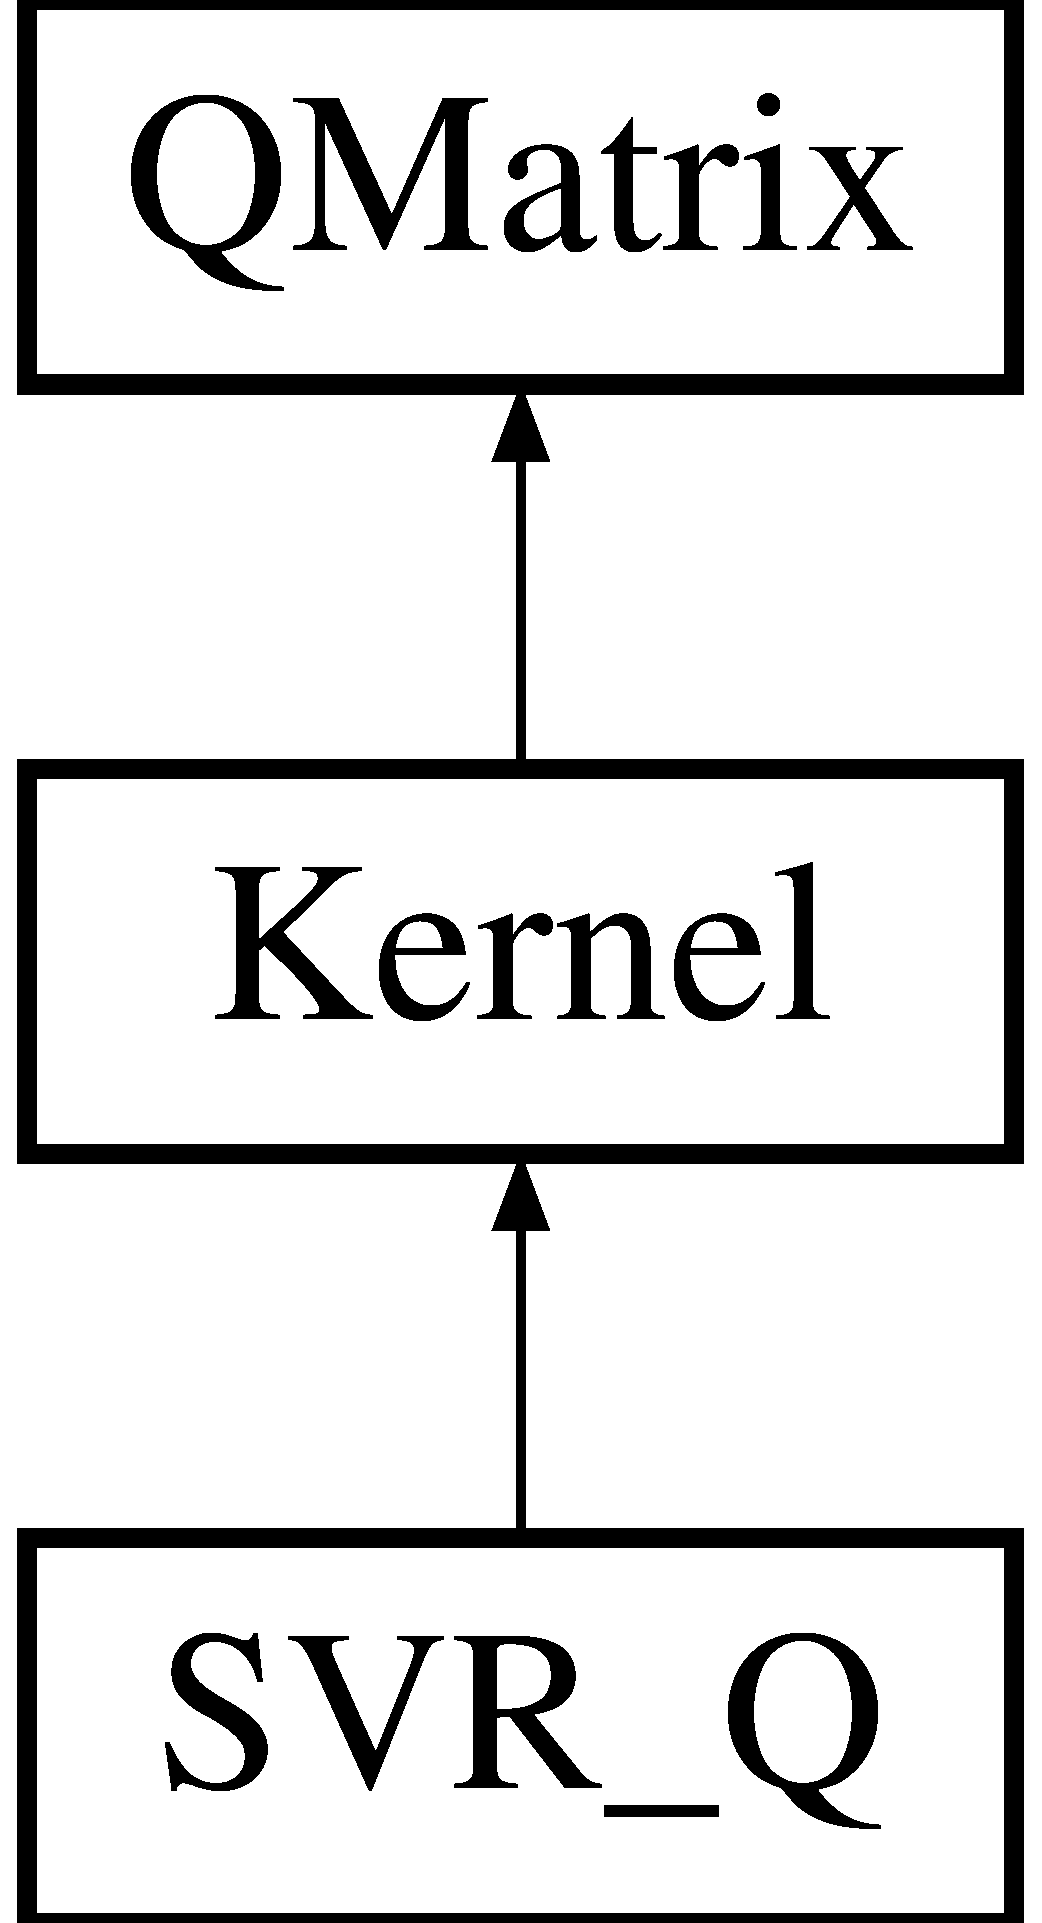
\includegraphics[height=3.000000cm]{classSVR__Q}
\end{center}
\end{figure}
\subsection*{Public Member Functions}
\begin{DoxyCompactItemize}
\item 
\hyperlink{classSVR__Q_a348978e0cce4c0bf503dc825241eb4ff}{S\+V\+R\+\_\+Q} (const \hyperlink{structsvm__problem}{svm\+\_\+problem} \&prob, const \hyperlink{structsvm__parameter}{svm\+\_\+parameter} \&param)
\item 
void \hyperlink{classSVR__Q_a9d3884f0c68f4ce18d47570e4a203405}{swap\+\_\+index} (int i, int j) const 
\item 
\hyperlink{svm__core_8cpp_a8755d90a54ecfb8d15051af3e0542592}{Qfloat} $\ast$ \hyperlink{classSVR__Q_aba55078d17e7815f093ffa154f3cee9d}{get\+\_\+Q} (int i, int len) const 
\item 
double $\ast$ \hyperlink{classSVR__Q_ac22ed5ce1b0bf6a900c3c8d631e77d76}{get\+\_\+\+QD} () const 
\item 
\hyperlink{classSVR__Q_a2a8efdc1fef68cc5bc9d0d2669d24e36}{$\sim$\+S\+V\+R\+\_\+Q} ()
\end{DoxyCompactItemize}
\subsection*{Additional Inherited Members}


\subsection{Constructor \& Destructor Documentation}
\index{S\+V\+R\+\_\+Q@{S\+V\+R\+\_\+Q}!S\+V\+R\+\_\+Q@{S\+V\+R\+\_\+Q}}
\index{S\+V\+R\+\_\+Q@{S\+V\+R\+\_\+Q}!S\+V\+R\+\_\+Q@{S\+V\+R\+\_\+Q}}
\subsubsection[{S\+V\+R\+\_\+\+Q(const svm\+\_\+problem \&prob, const svm\+\_\+parameter \&param)}]{\setlength{\rightskip}{0pt plus 5cm}S\+V\+R\+\_\+\+Q\+::\+S\+V\+R\+\_\+Q (
\begin{DoxyParamCaption}
\item[{const {\bf svm\+\_\+problem} \&}]{prob, }
\item[{const {\bf svm\+\_\+parameter} \&}]{param}
\end{DoxyParamCaption}
)\hspace{0.3cm}{\ttfamily [inline]}}\hypertarget{classSVR__Q_a348978e0cce4c0bf503dc825241eb4ff}{}\label{classSVR__Q_a348978e0cce4c0bf503dc825241eb4ff}
\index{S\+V\+R\+\_\+Q@{S\+V\+R\+\_\+Q}!````~S\+V\+R\+\_\+Q@{$\sim$\+S\+V\+R\+\_\+Q}}
\index{````~S\+V\+R\+\_\+Q@{$\sim$\+S\+V\+R\+\_\+Q}!S\+V\+R\+\_\+Q@{S\+V\+R\+\_\+Q}}
\subsubsection[{$\sim$\+S\+V\+R\+\_\+\+Q()}]{\setlength{\rightskip}{0pt plus 5cm}S\+V\+R\+\_\+\+Q\+::$\sim$\+S\+V\+R\+\_\+Q (
\begin{DoxyParamCaption}
{}
\end{DoxyParamCaption}
)\hspace{0.3cm}{\ttfamily [inline]}}\hypertarget{classSVR__Q_a2a8efdc1fef68cc5bc9d0d2669d24e36}{}\label{classSVR__Q_a2a8efdc1fef68cc5bc9d0d2669d24e36}


\subsection{Member Function Documentation}
\index{S\+V\+R\+\_\+Q@{S\+V\+R\+\_\+Q}!get\+\_\+Q@{get\+\_\+Q}}
\index{get\+\_\+Q@{get\+\_\+Q}!S\+V\+R\+\_\+Q@{S\+V\+R\+\_\+Q}}
\subsubsection[{get\+\_\+\+Q(int i, int len) const }]{\setlength{\rightskip}{0pt plus 5cm}{\bf Qfloat}$\ast$ S\+V\+R\+\_\+\+Q\+::get\+\_\+Q (
\begin{DoxyParamCaption}
\item[{int}]{i, }
\item[{int}]{len}
\end{DoxyParamCaption}
) const\hspace{0.3cm}{\ttfamily [inline]}, {\ttfamily [virtual]}}\hypertarget{classSVR__Q_aba55078d17e7815f093ffa154f3cee9d}{}\label{classSVR__Q_aba55078d17e7815f093ffa154f3cee9d}


Implements \hyperlink{classKernel_a02f328649424359b92b941f5219a6060}{Kernel}.

\index{S\+V\+R\+\_\+Q@{S\+V\+R\+\_\+Q}!get\+\_\+\+QD@{get\+\_\+\+QD}}
\index{get\+\_\+\+QD@{get\+\_\+\+QD}!S\+V\+R\+\_\+Q@{S\+V\+R\+\_\+Q}}
\subsubsection[{get\+\_\+\+Q\+D() const }]{\setlength{\rightskip}{0pt plus 5cm}double$\ast$ S\+V\+R\+\_\+\+Q\+::get\+\_\+\+QD (
\begin{DoxyParamCaption}
{}
\end{DoxyParamCaption}
) const\hspace{0.3cm}{\ttfamily [inline]}, {\ttfamily [virtual]}}\hypertarget{classSVR__Q_ac22ed5ce1b0bf6a900c3c8d631e77d76}{}\label{classSVR__Q_ac22ed5ce1b0bf6a900c3c8d631e77d76}


Implements \hyperlink{classKernel_a7bf9602583da1af48d15d19da69514ac}{Kernel}.

\index{S\+V\+R\+\_\+Q@{S\+V\+R\+\_\+Q}!swap\+\_\+index@{swap\+\_\+index}}
\index{swap\+\_\+index@{swap\+\_\+index}!S\+V\+R\+\_\+Q@{S\+V\+R\+\_\+Q}}
\subsubsection[{swap\+\_\+index(int i, int j) const }]{\setlength{\rightskip}{0pt plus 5cm}void S\+V\+R\+\_\+\+Q\+::swap\+\_\+index (
\begin{DoxyParamCaption}
\item[{int}]{i, }
\item[{int}]{j}
\end{DoxyParamCaption}
) const\hspace{0.3cm}{\ttfamily [inline]}, {\ttfamily [virtual]}}\hypertarget{classSVR__Q_a9d3884f0c68f4ce18d47570e4a203405}{}\label{classSVR__Q_a9d3884f0c68f4ce18d47570e4a203405}


Reimplemented from \hyperlink{classKernel_adca807c5584bc42fd098cd9eb1f19621}{Kernel}.



The documentation for this class was generated from the following file\+:\begin{DoxyCompactItemize}
\item 
src/\hyperlink{svm__core_8cpp}{svm\+\_\+core.\+cpp}\end{DoxyCompactItemize}

\chapter{File Documentation}
\hypertarget{CMakeCache_8txt}{}\section{build/\+C\+Make\+Cache.txt File Reference}
\label{CMakeCache_8txt}\index{build/\+C\+Make\+Cache.\+txt@{build/\+C\+Make\+Cache.\+txt}}

\hypertarget{CMakeCCompilerId_8c}{}\section{build/\+C\+Make\+Files/2.8.12.2/\+Compiler\+Id\+C/\+C\+Make\+C\+Compiler\+Id.c File Reference}
\label{CMakeCCompilerId_8c}\index{build/\+C\+Make\+Files/2.\+8.\+12.\+2/\+Compiler\+Id\+C/\+C\+Make\+C\+Compiler\+Id.\+c@{build/\+C\+Make\+Files/2.\+8.\+12.\+2/\+Compiler\+Id\+C/\+C\+Make\+C\+Compiler\+Id.\+c}}
\subsection*{Macros}
\begin{DoxyCompactItemize}
\item 
\#define \hyperlink{CMakeCCompilerId_8c_a81dee0709ded976b2e0319239f72d174}{C\+O\+M\+P\+I\+L\+E\+R\+\_\+\+ID}~\char`\"{}\char`\"{}
\item 
\#define \hyperlink{CMakeCCompilerId_8c_adbc5372f40838899018fadbc89bd588b}{P\+L\+A\+T\+F\+O\+R\+M\+\_\+\+ID}~\char`\"{}\char`\"{}
\item 
\#define \hyperlink{CMakeCCompilerId_8c_aba35d0d200deaeb06aee95ca297acb28}{A\+R\+C\+H\+I\+T\+E\+C\+T\+U\+R\+E\+\_\+\+ID}~\char`\"{}\char`\"{}
\item 
\#define \hyperlink{CMakeCCompilerId_8c_aac8ec3757ff33c1d78caa8ced06904d2}{D\+EC}(n)                                  
\item 
\#define \hyperlink{CMakeCCompilerId_8c_ad437e42b7da877bffc18f1965dae5765}{H\+EX}(n)                      
\end{DoxyCompactItemize}
\subsection*{Functions}
\begin{DoxyCompactItemize}
\item 
int \hyperlink{CMakeCCompilerId_8c_a0ddf1224851353fc92bfbff6f499fa97}{main} (int argc, char $\ast$argv\mbox{[}$\,$\mbox{]})
\end{DoxyCompactItemize}
\subsection*{Variables}
\begin{DoxyCompactItemize}
\item 
char const $\ast$ \hyperlink{CMakeCCompilerId_8c_a4b0efeb7a5d59313986b3a0390f050f6}{info\+\_\+compiler} = \char`\"{}I\+N\+FO\char`\"{} \char`\"{}\+:\char`\"{} \char`\"{}compiler\mbox{[}\char`\"{} C\+O\+M\+P\+I\+L\+E\+R\+\_\+\+ID \char`\"{}\mbox{]}\char`\"{}
\item 
char const $\ast$ \hyperlink{CMakeCCompilerId_8c_a2321403dee54ee23f0c2fa849c60f7d4}{info\+\_\+platform} = \char`\"{}I\+N\+FO\char`\"{} \char`\"{}\+:\char`\"{} \char`\"{}platform\mbox{[}\char`\"{} P\+L\+A\+T\+F\+O\+R\+M\+\_\+\+ID \char`\"{}\mbox{]}\char`\"{}
\item 
char const $\ast$ \hyperlink{CMakeCCompilerId_8c_a59647e99d304ed33b15cb284c27ed391}{info\+\_\+arch} = \char`\"{}I\+N\+FO\char`\"{} \char`\"{}\+:\char`\"{} \char`\"{}arch\mbox{[}\char`\"{} A\+R\+C\+H\+I\+T\+E\+C\+T\+U\+R\+E\+\_\+\+ID \char`\"{}\mbox{]}\char`\"{}
\end{DoxyCompactItemize}


\subsection{Macro Definition Documentation}
\index{C\+Make\+C\+Compiler\+Id.\+c@{C\+Make\+C\+Compiler\+Id.\+c}!A\+R\+C\+H\+I\+T\+E\+C\+T\+U\+R\+E\+\_\+\+ID@{A\+R\+C\+H\+I\+T\+E\+C\+T\+U\+R\+E\+\_\+\+ID}}
\index{A\+R\+C\+H\+I\+T\+E\+C\+T\+U\+R\+E\+\_\+\+ID@{A\+R\+C\+H\+I\+T\+E\+C\+T\+U\+R\+E\+\_\+\+ID}!C\+Make\+C\+Compiler\+Id.\+c@{C\+Make\+C\+Compiler\+Id.\+c}}
\subsubsection[{A\+R\+C\+H\+I\+T\+E\+C\+T\+U\+R\+E\+\_\+\+ID}]{\setlength{\rightskip}{0pt plus 5cm}\#define A\+R\+C\+H\+I\+T\+E\+C\+T\+U\+R\+E\+\_\+\+ID~\char`\"{}\char`\"{}}\hypertarget{CMakeCCompilerId_8c_aba35d0d200deaeb06aee95ca297acb28}{}\label{CMakeCCompilerId_8c_aba35d0d200deaeb06aee95ca297acb28}
\index{C\+Make\+C\+Compiler\+Id.\+c@{C\+Make\+C\+Compiler\+Id.\+c}!C\+O\+M\+P\+I\+L\+E\+R\+\_\+\+ID@{C\+O\+M\+P\+I\+L\+E\+R\+\_\+\+ID}}
\index{C\+O\+M\+P\+I\+L\+E\+R\+\_\+\+ID@{C\+O\+M\+P\+I\+L\+E\+R\+\_\+\+ID}!C\+Make\+C\+Compiler\+Id.\+c@{C\+Make\+C\+Compiler\+Id.\+c}}
\subsubsection[{C\+O\+M\+P\+I\+L\+E\+R\+\_\+\+ID}]{\setlength{\rightskip}{0pt plus 5cm}\#define C\+O\+M\+P\+I\+L\+E\+R\+\_\+\+ID~\char`\"{}\char`\"{}}\hypertarget{CMakeCCompilerId_8c_a81dee0709ded976b2e0319239f72d174}{}\label{CMakeCCompilerId_8c_a81dee0709ded976b2e0319239f72d174}
\index{C\+Make\+C\+Compiler\+Id.\+c@{C\+Make\+C\+Compiler\+Id.\+c}!D\+EC@{D\+EC}}
\index{D\+EC@{D\+EC}!C\+Make\+C\+Compiler\+Id.\+c@{C\+Make\+C\+Compiler\+Id.\+c}}
\subsubsection[{D\+EC}]{\setlength{\rightskip}{0pt plus 5cm}\#define D\+EC(
\begin{DoxyParamCaption}
\item[{}]{n}
\end{DoxyParamCaption}
)}\hypertarget{CMakeCCompilerId_8c_aac8ec3757ff33c1d78caa8ced06904d2}{}\label{CMakeCCompilerId_8c_aac8ec3757ff33c1d78caa8ced06904d2}
{\bfseries Value\+:}
\begin{DoxyCode}
(\textcolor{charliteral}{'0'} + (((n) / 10000000)%10)), \(\backslash\)
  (\textcolor{charliteral}{'0'} + (((n) / 1000000)%10)),  \(\backslash\)
  (\textcolor{charliteral}{'0'} + (((n) / 100000)%10)),   \(\backslash\)
  (\textcolor{charliteral}{'0'} + (((n) / 10000)%10)),    \(\backslash\)
  (\textcolor{charliteral}{'0'} + (((n) / 1000)%10)),     \(\backslash\)
  (\textcolor{charliteral}{'0'} + (((n) / 100)%10)),      \(\backslash\)
  (\textcolor{charliteral}{'0'} + (((n) / 10)%10)),       \(\backslash\)
  (\textcolor{charliteral}{'0'} +  ((n) % 10))
\end{DoxyCode}
\index{C\+Make\+C\+Compiler\+Id.\+c@{C\+Make\+C\+Compiler\+Id.\+c}!H\+EX@{H\+EX}}
\index{H\+EX@{H\+EX}!C\+Make\+C\+Compiler\+Id.\+c@{C\+Make\+C\+Compiler\+Id.\+c}}
\subsubsection[{H\+EX}]{\setlength{\rightskip}{0pt plus 5cm}\#define H\+EX(
\begin{DoxyParamCaption}
\item[{}]{n}
\end{DoxyParamCaption}
)}\hypertarget{CMakeCCompilerId_8c_ad437e42b7da877bffc18f1965dae5765}{}\label{CMakeCCompilerId_8c_ad437e42b7da877bffc18f1965dae5765}
{\bfseries Value\+:}
\begin{DoxyCode}
(\textcolor{charliteral}{'0'} + ((n)>>28 & 0xF)), \(\backslash\)
  (\textcolor{charliteral}{'0'} + ((n)>>24 & 0xF)), \(\backslash\)
  (\textcolor{charliteral}{'0'} + ((n)>>20 & 0xF)), \(\backslash\)
  (\textcolor{charliteral}{'0'} + ((n)>>16 & 0xF)), \(\backslash\)
  (\textcolor{charliteral}{'0'} + ((n)>>12 & 0xF)), \(\backslash\)
  (\textcolor{charliteral}{'0'} + ((n)>>8  & 0xF)), \(\backslash\)
  (\textcolor{charliteral}{'0'} + ((n)>>4  & 0xF)), \(\backslash\)
  (\textcolor{charliteral}{'0'} + ((n)     & 0xF))
\end{DoxyCode}
\index{C\+Make\+C\+Compiler\+Id.\+c@{C\+Make\+C\+Compiler\+Id.\+c}!P\+L\+A\+T\+F\+O\+R\+M\+\_\+\+ID@{P\+L\+A\+T\+F\+O\+R\+M\+\_\+\+ID}}
\index{P\+L\+A\+T\+F\+O\+R\+M\+\_\+\+ID@{P\+L\+A\+T\+F\+O\+R\+M\+\_\+\+ID}!C\+Make\+C\+Compiler\+Id.\+c@{C\+Make\+C\+Compiler\+Id.\+c}}
\subsubsection[{P\+L\+A\+T\+F\+O\+R\+M\+\_\+\+ID}]{\setlength{\rightskip}{0pt plus 5cm}\#define P\+L\+A\+T\+F\+O\+R\+M\+\_\+\+ID~\char`\"{}\char`\"{}}\hypertarget{CMakeCCompilerId_8c_adbc5372f40838899018fadbc89bd588b}{}\label{CMakeCCompilerId_8c_adbc5372f40838899018fadbc89bd588b}


\subsection{Function Documentation}
\index{C\+Make\+C\+Compiler\+Id.\+c@{C\+Make\+C\+Compiler\+Id.\+c}!main@{main}}
\index{main@{main}!C\+Make\+C\+Compiler\+Id.\+c@{C\+Make\+C\+Compiler\+Id.\+c}}
\subsubsection[{main(int argc, char $\ast$argv[])}]{\setlength{\rightskip}{0pt plus 5cm}int main (
\begin{DoxyParamCaption}
\item[{int}]{argc, }
\item[{char $\ast$}]{argv\mbox{[}$\,$\mbox{]}}
\end{DoxyParamCaption}
)}\hypertarget{CMakeCCompilerId_8c_a0ddf1224851353fc92bfbff6f499fa97}{}\label{CMakeCCompilerId_8c_a0ddf1224851353fc92bfbff6f499fa97}


\subsection{Variable Documentation}
\index{C\+Make\+C\+Compiler\+Id.\+c@{C\+Make\+C\+Compiler\+Id.\+c}!info\+\_\+arch@{info\+\_\+arch}}
\index{info\+\_\+arch@{info\+\_\+arch}!C\+Make\+C\+Compiler\+Id.\+c@{C\+Make\+C\+Compiler\+Id.\+c}}
\subsubsection[{info\+\_\+arch}]{\setlength{\rightskip}{0pt plus 5cm}char const$\ast$ info\+\_\+arch = \char`\"{}I\+N\+FO\char`\"{} \char`\"{}\+:\char`\"{} \char`\"{}arch\mbox{[}\char`\"{} A\+R\+C\+H\+I\+T\+E\+C\+T\+U\+R\+E\+\_\+\+ID \char`\"{}\mbox{]}\char`\"{}}\hypertarget{CMakeCCompilerId_8c_a59647e99d304ed33b15cb284c27ed391}{}\label{CMakeCCompilerId_8c_a59647e99d304ed33b15cb284c27ed391}
\index{C\+Make\+C\+Compiler\+Id.\+c@{C\+Make\+C\+Compiler\+Id.\+c}!info\+\_\+compiler@{info\+\_\+compiler}}
\index{info\+\_\+compiler@{info\+\_\+compiler}!C\+Make\+C\+Compiler\+Id.\+c@{C\+Make\+C\+Compiler\+Id.\+c}}
\subsubsection[{info\+\_\+compiler}]{\setlength{\rightskip}{0pt plus 5cm}char const$\ast$ info\+\_\+compiler = \char`\"{}I\+N\+FO\char`\"{} \char`\"{}\+:\char`\"{} \char`\"{}compiler\mbox{[}\char`\"{} C\+O\+M\+P\+I\+L\+E\+R\+\_\+\+ID \char`\"{}\mbox{]}\char`\"{}}\hypertarget{CMakeCCompilerId_8c_a4b0efeb7a5d59313986b3a0390f050f6}{}\label{CMakeCCompilerId_8c_a4b0efeb7a5d59313986b3a0390f050f6}
\index{C\+Make\+C\+Compiler\+Id.\+c@{C\+Make\+C\+Compiler\+Id.\+c}!info\+\_\+platform@{info\+\_\+platform}}
\index{info\+\_\+platform@{info\+\_\+platform}!C\+Make\+C\+Compiler\+Id.\+c@{C\+Make\+C\+Compiler\+Id.\+c}}
\subsubsection[{info\+\_\+platform}]{\setlength{\rightskip}{0pt plus 5cm}char const$\ast$ info\+\_\+platform = \char`\"{}I\+N\+FO\char`\"{} \char`\"{}\+:\char`\"{} \char`\"{}platform\mbox{[}\char`\"{} P\+L\+A\+T\+F\+O\+R\+M\+\_\+\+ID \char`\"{}\mbox{]}\char`\"{}}\hypertarget{CMakeCCompilerId_8c_a2321403dee54ee23f0c2fa849c60f7d4}{}\label{CMakeCCompilerId_8c_a2321403dee54ee23f0c2fa849c60f7d4}

\hypertarget{CMakeCXXCompilerId_8cpp}{}\section{build/\+C\+Make\+Files/2.8.12.2/\+Compiler\+Id\+C\+X\+X/\+C\+Make\+C\+X\+X\+Compiler\+Id.cpp File Reference}
\label{CMakeCXXCompilerId_8cpp}\index{build/\+C\+Make\+Files/2.\+8.\+12.\+2/\+Compiler\+Id\+C\+X\+X/\+C\+Make\+C\+X\+X\+Compiler\+Id.\+cpp@{build/\+C\+Make\+Files/2.\+8.\+12.\+2/\+Compiler\+Id\+C\+X\+X/\+C\+Make\+C\+X\+X\+Compiler\+Id.\+cpp}}
\subsection*{Macros}
\begin{DoxyCompactItemize}
\item 
\#define \hyperlink{CMakeCXXCompilerId_8cpp_a81dee0709ded976b2e0319239f72d174}{C\+O\+M\+P\+I\+L\+E\+R\+\_\+\+ID}~\char`\"{}\char`\"{}
\item 
\#define \hyperlink{CMakeCXXCompilerId_8cpp_adbc5372f40838899018fadbc89bd588b}{P\+L\+A\+T\+F\+O\+R\+M\+\_\+\+ID}~\char`\"{}\char`\"{}
\item 
\#define \hyperlink{CMakeCXXCompilerId_8cpp_aba35d0d200deaeb06aee95ca297acb28}{A\+R\+C\+H\+I\+T\+E\+C\+T\+U\+R\+E\+\_\+\+ID}~\char`\"{}\char`\"{}
\item 
\#define \hyperlink{CMakeCXXCompilerId_8cpp_aac8ec3757ff33c1d78caa8ced06904d2}{D\+EC}(n)                                  
\item 
\#define \hyperlink{CMakeCXXCompilerId_8cpp_ad437e42b7da877bffc18f1965dae5765}{H\+EX}(n)                      
\end{DoxyCompactItemize}
\subsection*{Functions}
\begin{DoxyCompactItemize}
\item 
int \hyperlink{CMakeCXXCompilerId_8cpp_a0ddf1224851353fc92bfbff6f499fa97}{main} (int argc, char $\ast$argv\mbox{[}$\,$\mbox{]})
\end{DoxyCompactItemize}
\subsection*{Variables}
\begin{DoxyCompactItemize}
\item 
char const $\ast$ \hyperlink{CMakeCXXCompilerId_8cpp_a4b0efeb7a5d59313986b3a0390f050f6}{info\+\_\+compiler} = \char`\"{}I\+N\+FO\char`\"{} \char`\"{}\+:\char`\"{} \char`\"{}compiler\mbox{[}\char`\"{} C\+O\+M\+P\+I\+L\+E\+R\+\_\+\+ID \char`\"{}\mbox{]}\char`\"{}
\item 
char const $\ast$ \hyperlink{CMakeCXXCompilerId_8cpp_a2321403dee54ee23f0c2fa849c60f7d4}{info\+\_\+platform} = \char`\"{}I\+N\+FO\char`\"{} \char`\"{}\+:\char`\"{} \char`\"{}platform\mbox{[}\char`\"{} P\+L\+A\+T\+F\+O\+R\+M\+\_\+\+ID \char`\"{}\mbox{]}\char`\"{}
\item 
char const $\ast$ \hyperlink{CMakeCXXCompilerId_8cpp_a59647e99d304ed33b15cb284c27ed391}{info\+\_\+arch} = \char`\"{}I\+N\+FO\char`\"{} \char`\"{}\+:\char`\"{} \char`\"{}arch\mbox{[}\char`\"{} A\+R\+C\+H\+I\+T\+E\+C\+T\+U\+R\+E\+\_\+\+ID \char`\"{}\mbox{]}\char`\"{}
\end{DoxyCompactItemize}


\subsection{Macro Definition Documentation}
\index{C\+Make\+C\+X\+X\+Compiler\+Id.\+cpp@{C\+Make\+C\+X\+X\+Compiler\+Id.\+cpp}!A\+R\+C\+H\+I\+T\+E\+C\+T\+U\+R\+E\+\_\+\+ID@{A\+R\+C\+H\+I\+T\+E\+C\+T\+U\+R\+E\+\_\+\+ID}}
\index{A\+R\+C\+H\+I\+T\+E\+C\+T\+U\+R\+E\+\_\+\+ID@{A\+R\+C\+H\+I\+T\+E\+C\+T\+U\+R\+E\+\_\+\+ID}!C\+Make\+C\+X\+X\+Compiler\+Id.\+cpp@{C\+Make\+C\+X\+X\+Compiler\+Id.\+cpp}}
\subsubsection[{A\+R\+C\+H\+I\+T\+E\+C\+T\+U\+R\+E\+\_\+\+ID}]{\setlength{\rightskip}{0pt plus 5cm}\#define A\+R\+C\+H\+I\+T\+E\+C\+T\+U\+R\+E\+\_\+\+ID~\char`\"{}\char`\"{}}\hypertarget{CMakeCXXCompilerId_8cpp_aba35d0d200deaeb06aee95ca297acb28}{}\label{CMakeCXXCompilerId_8cpp_aba35d0d200deaeb06aee95ca297acb28}
\index{C\+Make\+C\+X\+X\+Compiler\+Id.\+cpp@{C\+Make\+C\+X\+X\+Compiler\+Id.\+cpp}!C\+O\+M\+P\+I\+L\+E\+R\+\_\+\+ID@{C\+O\+M\+P\+I\+L\+E\+R\+\_\+\+ID}}
\index{C\+O\+M\+P\+I\+L\+E\+R\+\_\+\+ID@{C\+O\+M\+P\+I\+L\+E\+R\+\_\+\+ID}!C\+Make\+C\+X\+X\+Compiler\+Id.\+cpp@{C\+Make\+C\+X\+X\+Compiler\+Id.\+cpp}}
\subsubsection[{C\+O\+M\+P\+I\+L\+E\+R\+\_\+\+ID}]{\setlength{\rightskip}{0pt plus 5cm}\#define C\+O\+M\+P\+I\+L\+E\+R\+\_\+\+ID~\char`\"{}\char`\"{}}\hypertarget{CMakeCXXCompilerId_8cpp_a81dee0709ded976b2e0319239f72d174}{}\label{CMakeCXXCompilerId_8cpp_a81dee0709ded976b2e0319239f72d174}
\index{C\+Make\+C\+X\+X\+Compiler\+Id.\+cpp@{C\+Make\+C\+X\+X\+Compiler\+Id.\+cpp}!D\+EC@{D\+EC}}
\index{D\+EC@{D\+EC}!C\+Make\+C\+X\+X\+Compiler\+Id.\+cpp@{C\+Make\+C\+X\+X\+Compiler\+Id.\+cpp}}
\subsubsection[{D\+EC}]{\setlength{\rightskip}{0pt plus 5cm}\#define D\+EC(
\begin{DoxyParamCaption}
\item[{}]{n}
\end{DoxyParamCaption}
)}\hypertarget{CMakeCXXCompilerId_8cpp_aac8ec3757ff33c1d78caa8ced06904d2}{}\label{CMakeCXXCompilerId_8cpp_aac8ec3757ff33c1d78caa8ced06904d2}
{\bfseries Value\+:}
\begin{DoxyCode}
(\textcolor{charliteral}{'0'} + (((n) / 10000000)%10)), \(\backslash\)
  (\textcolor{charliteral}{'0'} + (((n) / 1000000)%10)),  \(\backslash\)
  (\textcolor{charliteral}{'0'} + (((n) / 100000)%10)),   \(\backslash\)
  (\textcolor{charliteral}{'0'} + (((n) / 10000)%10)),    \(\backslash\)
  (\textcolor{charliteral}{'0'} + (((n) / 1000)%10)),     \(\backslash\)
  (\textcolor{charliteral}{'0'} + (((n) / 100)%10)),      \(\backslash\)
  (\textcolor{charliteral}{'0'} + (((n) / 10)%10)),       \(\backslash\)
  (\textcolor{charliteral}{'0'} +  ((n) % 10))
\end{DoxyCode}
\index{C\+Make\+C\+X\+X\+Compiler\+Id.\+cpp@{C\+Make\+C\+X\+X\+Compiler\+Id.\+cpp}!H\+EX@{H\+EX}}
\index{H\+EX@{H\+EX}!C\+Make\+C\+X\+X\+Compiler\+Id.\+cpp@{C\+Make\+C\+X\+X\+Compiler\+Id.\+cpp}}
\subsubsection[{H\+EX}]{\setlength{\rightskip}{0pt plus 5cm}\#define H\+EX(
\begin{DoxyParamCaption}
\item[{}]{n}
\end{DoxyParamCaption}
)}\hypertarget{CMakeCXXCompilerId_8cpp_ad437e42b7da877bffc18f1965dae5765}{}\label{CMakeCXXCompilerId_8cpp_ad437e42b7da877bffc18f1965dae5765}
{\bfseries Value\+:}
\begin{DoxyCode}
(\textcolor{charliteral}{'0'} + ((n)>>28 & 0xF)), \(\backslash\)
  (\textcolor{charliteral}{'0'} + ((n)>>24 & 0xF)), \(\backslash\)
  (\textcolor{charliteral}{'0'} + ((n)>>20 & 0xF)), \(\backslash\)
  (\textcolor{charliteral}{'0'} + ((n)>>16 & 0xF)), \(\backslash\)
  (\textcolor{charliteral}{'0'} + ((n)>>12 & 0xF)), \(\backslash\)
  (\textcolor{charliteral}{'0'} + ((n)>>8  & 0xF)), \(\backslash\)
  (\textcolor{charliteral}{'0'} + ((n)>>4  & 0xF)), \(\backslash\)
  (\textcolor{charliteral}{'0'} + ((n)     & 0xF))
\end{DoxyCode}
\index{C\+Make\+C\+X\+X\+Compiler\+Id.\+cpp@{C\+Make\+C\+X\+X\+Compiler\+Id.\+cpp}!P\+L\+A\+T\+F\+O\+R\+M\+\_\+\+ID@{P\+L\+A\+T\+F\+O\+R\+M\+\_\+\+ID}}
\index{P\+L\+A\+T\+F\+O\+R\+M\+\_\+\+ID@{P\+L\+A\+T\+F\+O\+R\+M\+\_\+\+ID}!C\+Make\+C\+X\+X\+Compiler\+Id.\+cpp@{C\+Make\+C\+X\+X\+Compiler\+Id.\+cpp}}
\subsubsection[{P\+L\+A\+T\+F\+O\+R\+M\+\_\+\+ID}]{\setlength{\rightskip}{0pt plus 5cm}\#define P\+L\+A\+T\+F\+O\+R\+M\+\_\+\+ID~\char`\"{}\char`\"{}}\hypertarget{CMakeCXXCompilerId_8cpp_adbc5372f40838899018fadbc89bd588b}{}\label{CMakeCXXCompilerId_8cpp_adbc5372f40838899018fadbc89bd588b}


\subsection{Function Documentation}
\index{C\+Make\+C\+X\+X\+Compiler\+Id.\+cpp@{C\+Make\+C\+X\+X\+Compiler\+Id.\+cpp}!main@{main}}
\index{main@{main}!C\+Make\+C\+X\+X\+Compiler\+Id.\+cpp@{C\+Make\+C\+X\+X\+Compiler\+Id.\+cpp}}
\subsubsection[{main(int argc, char $\ast$argv[])}]{\setlength{\rightskip}{0pt plus 5cm}int main (
\begin{DoxyParamCaption}
\item[{int}]{argc, }
\item[{char $\ast$}]{argv\mbox{[}$\,$\mbox{]}}
\end{DoxyParamCaption}
)}\hypertarget{CMakeCXXCompilerId_8cpp_a0ddf1224851353fc92bfbff6f499fa97}{}\label{CMakeCXXCompilerId_8cpp_a0ddf1224851353fc92bfbff6f499fa97}


\subsection{Variable Documentation}
\index{C\+Make\+C\+X\+X\+Compiler\+Id.\+cpp@{C\+Make\+C\+X\+X\+Compiler\+Id.\+cpp}!info\+\_\+arch@{info\+\_\+arch}}
\index{info\+\_\+arch@{info\+\_\+arch}!C\+Make\+C\+X\+X\+Compiler\+Id.\+cpp@{C\+Make\+C\+X\+X\+Compiler\+Id.\+cpp}}
\subsubsection[{info\+\_\+arch}]{\setlength{\rightskip}{0pt plus 5cm}char const$\ast$ info\+\_\+arch = \char`\"{}I\+N\+FO\char`\"{} \char`\"{}\+:\char`\"{} \char`\"{}arch\mbox{[}\char`\"{} A\+R\+C\+H\+I\+T\+E\+C\+T\+U\+R\+E\+\_\+\+ID \char`\"{}\mbox{]}\char`\"{}}\hypertarget{CMakeCXXCompilerId_8cpp_a59647e99d304ed33b15cb284c27ed391}{}\label{CMakeCXXCompilerId_8cpp_a59647e99d304ed33b15cb284c27ed391}
\index{C\+Make\+C\+X\+X\+Compiler\+Id.\+cpp@{C\+Make\+C\+X\+X\+Compiler\+Id.\+cpp}!info\+\_\+compiler@{info\+\_\+compiler}}
\index{info\+\_\+compiler@{info\+\_\+compiler}!C\+Make\+C\+X\+X\+Compiler\+Id.\+cpp@{C\+Make\+C\+X\+X\+Compiler\+Id.\+cpp}}
\subsubsection[{info\+\_\+compiler}]{\setlength{\rightskip}{0pt plus 5cm}char const$\ast$ info\+\_\+compiler = \char`\"{}I\+N\+FO\char`\"{} \char`\"{}\+:\char`\"{} \char`\"{}compiler\mbox{[}\char`\"{} C\+O\+M\+P\+I\+L\+E\+R\+\_\+\+ID \char`\"{}\mbox{]}\char`\"{}}\hypertarget{CMakeCXXCompilerId_8cpp_a4b0efeb7a5d59313986b3a0390f050f6}{}\label{CMakeCXXCompilerId_8cpp_a4b0efeb7a5d59313986b3a0390f050f6}
\index{C\+Make\+C\+X\+X\+Compiler\+Id.\+cpp@{C\+Make\+C\+X\+X\+Compiler\+Id.\+cpp}!info\+\_\+platform@{info\+\_\+platform}}
\index{info\+\_\+platform@{info\+\_\+platform}!C\+Make\+C\+X\+X\+Compiler\+Id.\+cpp@{C\+Make\+C\+X\+X\+Compiler\+Id.\+cpp}}
\subsubsection[{info\+\_\+platform}]{\setlength{\rightskip}{0pt plus 5cm}char const$\ast$ info\+\_\+platform = \char`\"{}I\+N\+FO\char`\"{} \char`\"{}\+:\char`\"{} \char`\"{}platform\mbox{[}\char`\"{} P\+L\+A\+T\+F\+O\+R\+M\+\_\+\+ID \char`\"{}\mbox{]}\char`\"{}}\hypertarget{CMakeCXXCompilerId_8cpp_a2321403dee54ee23f0c2fa849c60f7d4}{}\label{CMakeCXXCompilerId_8cpp_a2321403dee54ee23f0c2fa849c60f7d4}

\hypertarget{conj_8dir_2link_8txt}{}\section{build/\+C\+Make\+Files/conj.dir/link.txt File Reference}
\label{conj_8dir_2link_8txt}\index{build/\+C\+Make\+Files/conj.\+dir/link.\+txt@{build/\+C\+Make\+Files/conj.\+dir/link.\+txt}}

\hypertarget{ex1_8dir_2link_8txt}{}\section{build/\+C\+Make\+Files/ex1.dir/link.txt File Reference}
\label{ex1_8dir_2link_8txt}\index{build/\+C\+Make\+Files/ex1.\+dir/link.\+txt@{build/\+C\+Make\+Files/ex1.\+dir/link.\+txt}}

\hypertarget{f1_8dir_2link_8txt}{}\section{build/\+C\+Make\+Files/f1.dir/link.txt File Reference}
\label{f1_8dir_2link_8txt}\index{build/\+C\+Make\+Files/f1.\+dir/link.\+txt@{build/\+C\+Make\+Files/f1.\+dir/link.\+txt}}

\hypertarget{f2_8dir_2link_8txt}{}\section{build/\+C\+Make\+Files/f2.dir/link.txt File Reference}
\label{f2_8dir_2link_8txt}\index{build/\+C\+Make\+Files/f2.\+dir/link.\+txt@{build/\+C\+Make\+Files/f2.\+dir/link.\+txt}}

\hypertarget{f3_8dir_2link_8txt}{}\section{build/\+C\+Make\+Files/f3.dir/link.txt File Reference}
\label{f3_8dir_2link_8txt}\index{build/\+C\+Make\+Files/f3.\+dir/link.\+txt@{build/\+C\+Make\+Files/f3.\+dir/link.\+txt}}

\hypertarget{z3test_8dir_2link_8txt}{}\section{build/\+C\+Make\+Files/z3test.dir/link.txt File Reference}
\label{z3test_8dir_2link_8txt}\index{build/\+C\+Make\+Files/z3test.\+dir/link.\+txt@{build/\+C\+Make\+Files/z3test.\+dir/link.\+txt}}

\hypertarget{TargetDirectories_8txt}{}\section{build/\+C\+Make\+Files/\+Target\+Directories.txt File Reference}
\label{TargetDirectories_8txt}\index{build/\+C\+Make\+Files/\+Target\+Directories.\+txt@{build/\+C\+Make\+Files/\+Target\+Directories.\+txt}}

\hypertarget{CMakeLists_8txt}{}\section{C\+Make\+Lists.\+txt File Reference}
\label{CMakeLists_8txt}\index{C\+Make\+Lists.\+txt@{C\+Make\+Lists.\+txt}}

\hypertarget{color_8h}{}\section{include/color.h File Reference}
\label{color_8h}\index{include/color.\+h@{include/color.\+h}}


Provide support for colorful console ouput.  


{\ttfamily \#include $<$iostream$>$}\\*
\subsection*{Enumerations}
\begin{DoxyCompactItemize}
\item 
enum \hyperlink{color_8h_a37dbdc30935031c05304482e1be89d8f}{color} \{ \\*
\hyperlink{color_8h_a37dbdc30935031c05304482e1be89d8faf80f9a890089d211842d59625e561f88}{R\+ED} = 0, 
\hyperlink{color_8h_a37dbdc30935031c05304482e1be89d8fae735a848bf82163a19236ead1c3ef2d2}{Y\+E\+L\+L\+OW}, 
\hyperlink{color_8h_a37dbdc30935031c05304482e1be89d8faa60bd322f93178d68184e30e162571ca}{G\+R\+E\+EN}, 
\hyperlink{color_8h_a37dbdc30935031c05304482e1be89d8fa35d6719cb4d7577c031b3d79057a1b79}{B\+L\+UE}, 
\\*
\hyperlink{color_8h_a37dbdc30935031c05304482e1be89d8fa283fc479650da98250635b9c3c0e7e50}{W\+H\+I\+TE}
 \}\begin{DoxyCompactList}\small\item\em This enumeration contains all the colors predifined in project. Here we only introduce R\+ED, Y\+E\+L\+L\+OW, G\+R\+E\+EN, B\+L\+UE, W\+H\+I\+TE which is enough for our output. You can import more color if you want. \end{DoxyCompactList}
\end{DoxyCompactItemize}
\subsection*{Functions}
\begin{DoxyCompactItemize}
\item 
void \hyperlink{color_8h_a0665e13d18d97e69df7b6adf4ec3b2ad}{set\+\_\+console\+\_\+color} (std\+::ostream \&out, int \hyperlink{color_8h_a37dbdc30935031c05304482e1be89d8f}{color}=\hyperlink{color_8h_a37dbdc30935031c05304482e1be89d8fae735a848bf82163a19236ead1c3ef2d2}{Y\+E\+L\+L\+OW})
\begin{DoxyCompactList}\small\item\em This function sets the given stream to the given color, Y\+E\+L\+L\+OW is default. \end{DoxyCompactList}\item 
void \hyperlink{color_8h_ab25f05cf8d2080aa8b7103d7b77c44cd}{unset\+\_\+console\+\_\+color} (std\+::ostream \&out)
\begin{DoxyCompactList}\small\item\em This function sets the console color back to origin setting, not the previous setting. By origin, we mean black background, white foreground, no strong comparision. \end{DoxyCompactList}\end{DoxyCompactItemize}


\subsection{Detailed Description}
Provide support for colorful console ouput. 

This file contains the necessary function support for colorful console text output. The usage is also simple. Before you output something, call function set\+\_\+console\+\_\+color. And remember to call unset\+\_\+console\+\_\+color after your output.

\begin{DoxyAuthor}{Author}
Li Jiaying 
\end{DoxyAuthor}
\begin{DoxyRefDesc}{Bug}
\item[\hyperlink{bug__bug000001}{Bug}]unset\+\_\+console\+\_\+color is set the console back to black background, white forground, no strong comparision instead of the previous setting. \end{DoxyRefDesc}


\subsection{Enumeration Type Documentation}
\index{color.\+h@{color.\+h}!color@{color}}
\index{color@{color}!color.\+h@{color.\+h}}
\subsubsection[{color}]{\setlength{\rightskip}{0pt plus 5cm}enum {\bf color}}\hypertarget{color_8h_a37dbdc30935031c05304482e1be89d8f}{}\label{color_8h_a37dbdc30935031c05304482e1be89d8f}


This enumeration contains all the colors predifined in project. Here we only introduce R\+ED, Y\+E\+L\+L\+OW, G\+R\+E\+EN, B\+L\+UE, W\+H\+I\+TE which is enough for our output. You can import more color if you want. 

\begin{Desc}
\item[Enumerator]\par
\begin{description}
\index{R\+ED@{R\+ED}!color.\+h@{color.\+h}}\index{color.\+h@{color.\+h}!R\+ED@{R\+ED}}\item[{\em 
R\+ED\hypertarget{color_8h_a37dbdc30935031c05304482e1be89d8faf80f9a890089d211842d59625e561f88}{}\label{color_8h_a37dbdc30935031c05304482e1be89d8faf80f9a890089d211842d59625e561f88}
}]\index{Y\+E\+L\+L\+OW@{Y\+E\+L\+L\+OW}!color.\+h@{color.\+h}}\index{color.\+h@{color.\+h}!Y\+E\+L\+L\+OW@{Y\+E\+L\+L\+OW}}\item[{\em 
Y\+E\+L\+L\+OW\hypertarget{color_8h_a37dbdc30935031c05304482e1be89d8fae735a848bf82163a19236ead1c3ef2d2}{}\label{color_8h_a37dbdc30935031c05304482e1be89d8fae735a848bf82163a19236ead1c3ef2d2}
}]\index{G\+R\+E\+EN@{G\+R\+E\+EN}!color.\+h@{color.\+h}}\index{color.\+h@{color.\+h}!G\+R\+E\+EN@{G\+R\+E\+EN}}\item[{\em 
G\+R\+E\+EN\hypertarget{color_8h_a37dbdc30935031c05304482e1be89d8faa60bd322f93178d68184e30e162571ca}{}\label{color_8h_a37dbdc30935031c05304482e1be89d8faa60bd322f93178d68184e30e162571ca}
}]\index{B\+L\+UE@{B\+L\+UE}!color.\+h@{color.\+h}}\index{color.\+h@{color.\+h}!B\+L\+UE@{B\+L\+UE}}\item[{\em 
B\+L\+UE\hypertarget{color_8h_a37dbdc30935031c05304482e1be89d8fa35d6719cb4d7577c031b3d79057a1b79}{}\label{color_8h_a37dbdc30935031c05304482e1be89d8fa35d6719cb4d7577c031b3d79057a1b79}
}]\index{W\+H\+I\+TE@{W\+H\+I\+TE}!color.\+h@{color.\+h}}\index{color.\+h@{color.\+h}!W\+H\+I\+TE@{W\+H\+I\+TE}}\item[{\em 
W\+H\+I\+TE\hypertarget{color_8h_a37dbdc30935031c05304482e1be89d8fa283fc479650da98250635b9c3c0e7e50}{}\label{color_8h_a37dbdc30935031c05304482e1be89d8fa283fc479650da98250635b9c3c0e7e50}
}]\end{description}
\end{Desc}


\subsection{Function Documentation}
\index{color.\+h@{color.\+h}!set\+\_\+console\+\_\+color@{set\+\_\+console\+\_\+color}}
\index{set\+\_\+console\+\_\+color@{set\+\_\+console\+\_\+color}!color.\+h@{color.\+h}}
\subsubsection[{set\+\_\+console\+\_\+color(std\+::ostream \&out, int color=\+Y\+E\+L\+L\+O\+W)}]{\setlength{\rightskip}{0pt plus 5cm}void set\+\_\+console\+\_\+color (
\begin{DoxyParamCaption}
\item[{std\+::ostream \&}]{out, }
\item[{int}]{color = {\ttfamily {\bf Y\+E\+L\+L\+OW}}}
\end{DoxyParamCaption}
)}\hypertarget{color_8h_a0665e13d18d97e69df7b6adf4ec3b2ad}{}\label{color_8h_a0665e13d18d97e69df7b6adf4ec3b2ad}


This function sets the given stream to the given color, Y\+E\+L\+L\+OW is default. 


\begin{DoxyParams}{Parameters}
{\em out} & The ostream to be changed, defines which stream you want to set \\
\hline
{\em color} & The Color to set. Y\+E\+L\+L\+OW by default. \\
\hline
\end{DoxyParams}
\index{color.\+h@{color.\+h}!unset\+\_\+console\+\_\+color@{unset\+\_\+console\+\_\+color}}
\index{unset\+\_\+console\+\_\+color@{unset\+\_\+console\+\_\+color}!color.\+h@{color.\+h}}
\subsubsection[{unset\+\_\+console\+\_\+color(std\+::ostream \&out)}]{\setlength{\rightskip}{0pt plus 5cm}void unset\+\_\+console\+\_\+color (
\begin{DoxyParamCaption}
\item[{std\+::ostream \&}]{out}
\end{DoxyParamCaption}
)}\hypertarget{color_8h_ab25f05cf8d2080aa8b7103d7b77c44cd}{}\label{color_8h_ab25f05cf8d2080aa8b7103d7b77c44cd}


This function sets the console color back to origin setting, not the previous setting. By origin, we mean black background, white foreground, no strong comparision. 


\hypertarget{config_8h}{}\section{include/config.h File Reference}
\label{config_8h}\index{include/config.\+h@{include/config.\+h}}


Provide most configuration information for whole project.  


\subsection*{Macros}
\begin{DoxyCompactItemize}
\item 
\#define \hyperlink{config_8h_a1d6565a8ececd15de44965eec4790919}{V\+A\+RS}~2
\begin{DoxyCompactList}\small\item\em defines the number of paramenters by a given loop,\textbackslash{} This also is the number of parameters we need to record for processing. This should be set in /\+C\+Make\+Lists.txt file If it is not set correctly, you may come across a runtime error \end{DoxyCompactList}\item 
\#define \hyperlink{config_8h_a9c7b069fee3c8184e14a7de8e5da2dc6}{P\+R\+E\+C\+I\+S\+I\+ON}~3
\begin{DoxyCompactList}\small\item\em is a integer, which defines precision as pow(10, -\/\+P\+R\+E\+C\+I\+S\+I\+ON) This should be set in /\+C\+Make\+Lists.txt file You\textquotesingle{}d better set this value in a scope \mbox{[}1, 12\mbox{]} \end{DoxyCompactList}\end{DoxyCompactItemize}
\subsection*{Functions}
\begin{DoxyCompactItemize}
\item 
bool \hyperlink{config_8h_a8c5bae50d678b664c26f20fe2714b643}{register\+\_\+program} (int($\ast$func)(int $\ast$), const char $\ast$func\+\_\+name=0)
\begin{DoxyCompactList}\small\item\em This function register the test program to the framework. \end{DoxyCompactList}\end{DoxyCompactItemize}
\subsection*{Variables}
\begin{DoxyCompactItemize}
\item 
int($\ast$ \hyperlink{config_8h_aa4ddce24d31048c0e720e8a881102639}{target\+\_\+program} )(int $\ast$)
\begin{DoxyCompactList}\small\item\em The pointer to test program, DO N\+OT assign directly Call register\+\_\+program to set its value. \end{DoxyCompactList}\item 
const int \hyperlink{config_8h_ab763a0a7202006efe98fe9953784e6a9}{max\+\_\+items} = 100000
\begin{DoxyCompactList}\small\item\em defines the initial max number items contains by states set. Better to be a number larger than 1000 \end{DoxyCompactList}\item 
const int \hyperlink{config_8h_a9cdc06717fd3c453855e0f1236107749}{init\+\_\+exes} = 6 $\ast$ \hyperlink{config_8h_a1d6565a8ececd15de44965eec4790919}{V\+A\+RS}
\begin{DoxyCompactList}\small\item\em defines the number of tests runs initially. Should be a positive integer. \end{DoxyCompactList}\item 
const int \hyperlink{config_8h_af9899f4090dc9468966227cb6af15906}{after\+\_\+exes} = 4 $\ast$ \hyperlink{config_8h_a1d6565a8ececd15de44965eec4790919}{V\+A\+RS}
\begin{DoxyCompactList}\small\item\em defines the number of tests runs after the first time. Should be a positive integer. \end{DoxyCompactList}\item 
const int \hyperlink{config_8h_a13c279f1a09e02e6224a93ee6aadae5b}{random\+\_\+exes} = 2
\begin{DoxyCompactList}\small\item\em defines the number of random tests runs each time, which is used to avoid bias caused by tests picking chioce. Should be a non-\/negative integer. \end{DoxyCompactList}\item 
const int \hyperlink{config_8h_a7a2c49f1d0b87e326420efb7e71cb89f}{max\+\_\+iter} = 32
\begin{DoxyCompactList}\small\item\em defines the max number of iterations tried by machine learning algorithm, Should be a positive integer. Usually set between 8-\/128 \end{DoxyCompactList}\end{DoxyCompactItemize}


\subsection{Detailed Description}
Provide most configuration information for whole project. 

This file contains most of the setting which are used to customize the project.

\begin{DoxyAuthor}{Author}
Li Jiaying 
\end{DoxyAuthor}
\begin{DoxyRefDesc}{Bug}
\item[\hyperlink{bug__bug000002}{Bug}]No known bugs. \end{DoxyRefDesc}


\subsection{Macro Definition Documentation}
\index{config.\+h@{config.\+h}!P\+R\+E\+C\+I\+S\+I\+ON@{P\+R\+E\+C\+I\+S\+I\+ON}}
\index{P\+R\+E\+C\+I\+S\+I\+ON@{P\+R\+E\+C\+I\+S\+I\+ON}!config.\+h@{config.\+h}}
\subsubsection[{P\+R\+E\+C\+I\+S\+I\+ON}]{\setlength{\rightskip}{0pt plus 5cm}\#define P\+R\+E\+C\+I\+S\+I\+ON~3}\hypertarget{config_8h_a9c7b069fee3c8184e14a7de8e5da2dc6}{}\label{config_8h_a9c7b069fee3c8184e14a7de8e5da2dc6}


is a integer, which defines precision as pow(10, -\/\+P\+R\+E\+C\+I\+S\+I\+ON) This should be set in /\+C\+Make\+Lists.txt file You\textquotesingle{}d better set this value in a scope \mbox{[}1, 12\mbox{]} 

\index{config.\+h@{config.\+h}!V\+A\+RS@{V\+A\+RS}}
\index{V\+A\+RS@{V\+A\+RS}!config.\+h@{config.\+h}}
\subsubsection[{V\+A\+RS}]{\setlength{\rightskip}{0pt plus 5cm}\#define V\+A\+RS~2}\hypertarget{config_8h_a1d6565a8ececd15de44965eec4790919}{}\label{config_8h_a1d6565a8ececd15de44965eec4790919}


defines the number of paramenters by a given loop,\textbackslash{} This also is the number of parameters we need to record for processing. This should be set in /\+C\+Make\+Lists.txt file If it is not set correctly, you may come across a runtime error 



\subsection{Function Documentation}
\index{config.\+h@{config.\+h}!register\+\_\+program@{register\+\_\+program}}
\index{register\+\_\+program@{register\+\_\+program}!config.\+h@{config.\+h}}
\subsubsection[{register\+\_\+program(int($\ast$func)(int $\ast$), const char $\ast$func\+\_\+name=0)}]{\setlength{\rightskip}{0pt plus 5cm}bool register\+\_\+program (
\begin{DoxyParamCaption}
\item[{int($\ast$)(int $\ast$)}]{func, }
\item[{const char $\ast$}]{func\+\_\+name = {\ttfamily 0}}
\end{DoxyParamCaption}
)}\hypertarget{config_8h_a8c5bae50d678b664c26f20fe2714b643}{}\label{config_8h_a8c5bae50d678b664c26f20fe2714b643}


This function register the test program to the framework. 


\begin{DoxyParams}{Parameters}
{\em func} & The function to be tested It involves a small validation test on the given function. \\
\hline
{\em fun\+\_\+name} & defines the function name, can be ignored, or set to N\+U\+LL \\
\hline
\end{DoxyParams}
\begin{DoxyReturn}{Returns}
a boolean value false only when the given function is not valid. 
\end{DoxyReturn}


\subsection{Variable Documentation}
\index{config.\+h@{config.\+h}!after\+\_\+exes@{after\+\_\+exes}}
\index{after\+\_\+exes@{after\+\_\+exes}!config.\+h@{config.\+h}}
\subsubsection[{after\+\_\+exes}]{\setlength{\rightskip}{0pt plus 5cm}const int after\+\_\+exes = 4 $\ast$ {\bf V\+A\+RS}}\hypertarget{config_8h_af9899f4090dc9468966227cb6af15906}{}\label{config_8h_af9899f4090dc9468966227cb6af15906}


defines the number of tests runs after the first time. Should be a positive integer. 

\index{config.\+h@{config.\+h}!init\+\_\+exes@{init\+\_\+exes}}
\index{init\+\_\+exes@{init\+\_\+exes}!config.\+h@{config.\+h}}
\subsubsection[{init\+\_\+exes}]{\setlength{\rightskip}{0pt plus 5cm}const int init\+\_\+exes = 6 $\ast$ {\bf V\+A\+RS}}\hypertarget{config_8h_a9cdc06717fd3c453855e0f1236107749}{}\label{config_8h_a9cdc06717fd3c453855e0f1236107749}


defines the number of tests runs initially. Should be a positive integer. 

\index{config.\+h@{config.\+h}!max\+\_\+items@{max\+\_\+items}}
\index{max\+\_\+items@{max\+\_\+items}!config.\+h@{config.\+h}}
\subsubsection[{max\+\_\+items}]{\setlength{\rightskip}{0pt plus 5cm}const int max\+\_\+items = 100000}\hypertarget{config_8h_ab763a0a7202006efe98fe9953784e6a9}{}\label{config_8h_ab763a0a7202006efe98fe9953784e6a9}


defines the initial max number items contains by states set. Better to be a number larger than 1000 

\index{config.\+h@{config.\+h}!max\+\_\+iter@{max\+\_\+iter}}
\index{max\+\_\+iter@{max\+\_\+iter}!config.\+h@{config.\+h}}
\subsubsection[{max\+\_\+iter}]{\setlength{\rightskip}{0pt plus 5cm}const int max\+\_\+iter = 32}\hypertarget{config_8h_a7a2c49f1d0b87e326420efb7e71cb89f}{}\label{config_8h_a7a2c49f1d0b87e326420efb7e71cb89f}


defines the max number of iterations tried by machine learning algorithm, Should be a positive integer. Usually set between 8-\/128 

\index{config.\+h@{config.\+h}!random\+\_\+exes@{random\+\_\+exes}}
\index{random\+\_\+exes@{random\+\_\+exes}!config.\+h@{config.\+h}}
\subsubsection[{random\+\_\+exes}]{\setlength{\rightskip}{0pt plus 5cm}const int random\+\_\+exes = 2}\hypertarget{config_8h_a13c279f1a09e02e6224a93ee6aadae5b}{}\label{config_8h_a13c279f1a09e02e6224a93ee6aadae5b}


defines the number of random tests runs each time, which is used to avoid bias caused by tests picking chioce. Should be a non-\/negative integer. 

\index{config.\+h@{config.\+h}!target\+\_\+program@{target\+\_\+program}}
\index{target\+\_\+program@{target\+\_\+program}!config.\+h@{config.\+h}}
\subsubsection[{target\+\_\+program}]{\setlength{\rightskip}{0pt plus 5cm}int($\ast$ target\+\_\+program) (int $\ast$)}\hypertarget{config_8h_aa4ddce24d31048c0e720e8a881102639}{}\label{config_8h_aa4ddce24d31048c0e720e8a881102639}


The pointer to test program, DO N\+OT assign directly Call register\+\_\+program to set its value. 


\hypertarget{equation_8h}{}\section{include/equation.h File Reference}
\label{equation_8h}\index{include/equation.\+h@{include/equation.\+h}}
{\ttfamily \#include \char`\"{}config.\+h\char`\"{}}\\*
{\ttfamily \#include $<$cmath$>$}\\*
{\ttfamily \#include $<$cfloat$>$}\\*
{\ttfamily \#include $<$stdarg.\+h$>$}\\*
{\ttfamily \#include $<$cstdlib$>$}\\*
{\ttfamily \#include $<$iostream$>$}\\*
{\ttfamily \#include $<$iomanip$>$}\\*
\subsection*{Data Structures}
\begin{DoxyCompactItemize}
\item 
class \hyperlink{classSolution}{Solution}
\item 
class \hyperlink{classEquation}{Equation}
\end{DoxyCompactItemize}
\subsection*{Variables}
\begin{DoxyCompactItemize}
\item 
int \hyperlink{equation_8h_ab928cec994c1d232e72009cfa90ac963}{maxv}
\item 
int \hyperlink{equation_8h_a85cc72fa9528a0cf48804027b7e943ec}{minv}
\end{DoxyCompactItemize}


\subsection{Variable Documentation}
\index{equation.\+h@{equation.\+h}!maxv@{maxv}}
\index{maxv@{maxv}!equation.\+h@{equation.\+h}}
\subsubsection[{maxv}]{\setlength{\rightskip}{0pt plus 5cm}int maxv}\hypertarget{equation_8h_ab928cec994c1d232e72009cfa90ac963}{}\label{equation_8h_ab928cec994c1d232e72009cfa90ac963}
\index{equation.\+h@{equation.\+h}!minv@{minv}}
\index{minv@{minv}!equation.\+h@{equation.\+h}}
\subsubsection[{minv}]{\setlength{\rightskip}{0pt plus 5cm}int minv}\hypertarget{equation_8h_a85cc72fa9528a0cf48804027b7e943ec}{}\label{equation_8h_a85cc72fa9528a0cf48804027b7e943ec}

\hypertarget{iif_8h}{}\section{include/iif.h File Reference}
\label{iif_8h}\index{include/iif.\+h@{include/iif.\+h}}
{\ttfamily \#include \char`\"{}config.\+h\char`\"{}}\\*
{\ttfamily \#include \char`\"{}instrumentation.\+h\char`\"{}}\\*
{\ttfamily \#include \char`\"{}ml\+\_\+algo.\+h\char`\"{}}\\*
{\ttfamily \#include \char`\"{}svm.\+h\char`\"{}}\\*
{\ttfamily \#include \char`\"{}svm\+\_\+i.\+h\char`\"{}}\\*
{\ttfamily \#include \char`\"{}color.\+h\char`\"{}}\\*
{\ttfamily \#include \char`\"{}equation.\+h\char`\"{}}\\*
{\ttfamily \#include \char`\"{}states.\+h\char`\"{}}\\*
{\ttfamily \#include \char`\"{}iif\+\_\+learn.\+h\char`\"{}}\\*
{\ttfamily \#include \char`\"{}iif\+\_\+svm\+\_\+learn.\+h\char`\"{}}\\*
{\ttfamily \#include \char`\"{}iif\+\_\+svm\+\_\+i\+\_\+learn.\+h\char`\"{}}\\*
{\ttfamily \#include \char`\"{}iif\+\_\+assert.\+h\char`\"{}}\\*
{\ttfamily \#include $<$iostream$>$}\\*
{\ttfamily \#include $<$float.\+h$>$}\\*
{\ttfamily \#include $<$string.\+h$>$}\\*
{\ttfamily \#include $<$assert.\+h$>$}\\*
{\ttfamily \#include $<$cstdlib$>$}\\*
\subsection*{Variables}
\begin{DoxyCompactItemize}
\item 
int \hyperlink{iif_8h_a85cc72fa9528a0cf48804027b7e943ec}{minv}
\item 
int \hyperlink{iif_8h_ab928cec994c1d232e72009cfa90ac963}{maxv}
\end{DoxyCompactItemize}


\subsection{Variable Documentation}
\index{iif.\+h@{iif.\+h}!maxv@{maxv}}
\index{maxv@{maxv}!iif.\+h@{iif.\+h}}
\subsubsection[{maxv}]{\setlength{\rightskip}{0pt plus 5cm}int maxv}\hypertarget{iif_8h_ab928cec994c1d232e72009cfa90ac963}{}\label{iif_8h_ab928cec994c1d232e72009cfa90ac963}
\index{iif.\+h@{iif.\+h}!minv@{minv}}
\index{minv@{minv}!iif.\+h@{iif.\+h}}
\subsubsection[{minv}]{\setlength{\rightskip}{0pt plus 5cm}int minv}\hypertarget{iif_8h_a85cc72fa9528a0cf48804027b7e943ec}{}\label{iif_8h_a85cc72fa9528a0cf48804027b7e943ec}

\hypertarget{iif__assert_8h}{}\section{include/iif\+\_\+assert.h File Reference}
\label{iif__assert_8h}\index{include/iif\+\_\+assert.\+h@{include/iif\+\_\+assert.\+h}}
\subsection*{Macros}
\begin{DoxyCompactItemize}
\item 
\#define \hyperlink{iif__assert_8h_a77c691e35bf160a48b865e93073dd759}{iif\+\_\+assume}(expr)
\item 
\#define \hyperlink{iif__assert_8h_af22e31973faa40470618b5f370326651}{iif\+\_\+assert}(expr)
\end{DoxyCompactItemize}
\subsection*{Variables}
\begin{DoxyCompactItemize}
\item 
bool \hyperlink{iif__assert_8h_a73db7f19ba8224c4530f45fd832ef42b}{\+\_\+passP}
\item 
bool \hyperlink{iif__assert_8h_a87e762b3355fdc144393f0936c14f8ca}{\+\_\+passQ}
\item 
int \hyperlink{iif__assert_8h_a552efb21fe547d54565d8379dc8a95bc}{assume\+\_\+times}
\item 
int \hyperlink{iif__assert_8h_a3b38e8ff0d716993240c2bbc5c25a59e}{assert\+\_\+times}
\end{DoxyCompactItemize}


\subsection{Macro Definition Documentation}
\index{iif\+\_\+assert.\+h@{iif\+\_\+assert.\+h}!iif\+\_\+assert@{iif\+\_\+assert}}
\index{iif\+\_\+assert@{iif\+\_\+assert}!iif\+\_\+assert.\+h@{iif\+\_\+assert.\+h}}
\subsubsection[{iif\+\_\+assert}]{\setlength{\rightskip}{0pt plus 5cm}\#define iif\+\_\+assert(
\begin{DoxyParamCaption}
\item[{}]{expr}
\end{DoxyParamCaption}
)}\hypertarget{iif__assert_8h_af22e31973faa40470618b5f370326651}{}\label{iif__assert_8h_af22e31973faa40470618b5f370326651}
{\bfseries Value\+:}
\begin{DoxyCode}
\textcolor{keywordflow}{do} \{ \hyperlink{iif__assert_8h_a87e762b3355fdc144393f0936c14f8ca}{\(\backslash\)}
\hyperlink{iif__assert_8h_a87e762b3355fdc144393f0936c14f8ca}{    \_passQ} = (expr)? \textcolor{keyword}{true} : \textcolor{keyword}{false};\hyperlink{iif__assert_8h_a3b38e8ff0d716993240c2bbc5c25a59e}{\(\backslash\)}
\hyperlink{iif__assert_8h_a3b38e8ff0d716993240c2bbc5c25a59e}{    assert\_times}++;\(\backslash\)
\} \textcolor{keywordflow}{while}(0)
\end{DoxyCode}
\index{iif\+\_\+assert.\+h@{iif\+\_\+assert.\+h}!iif\+\_\+assume@{iif\+\_\+assume}}
\index{iif\+\_\+assume@{iif\+\_\+assume}!iif\+\_\+assert.\+h@{iif\+\_\+assert.\+h}}
\subsubsection[{iif\+\_\+assume}]{\setlength{\rightskip}{0pt plus 5cm}\#define iif\+\_\+assume(
\begin{DoxyParamCaption}
\item[{}]{expr}
\end{DoxyParamCaption}
)}\hypertarget{iif__assert_8h_a77c691e35bf160a48b865e93073dd759}{}\label{iif__assert_8h_a77c691e35bf160a48b865e93073dd759}
{\bfseries Value\+:}
\begin{DoxyCode}
\textcolor{keywordflow}{do} \{ \hyperlink{iif__assert_8h_a73db7f19ba8224c4530f45fd832ef42b}{\(\backslash\)}
\hyperlink{iif__assert_8h_a73db7f19ba8224c4530f45fd832ef42b}{    \_passP} = (expr)? \textcolor{keyword}{true} : \textcolor{keyword}{false};\hyperlink{iif__assert_8h_a552efb21fe547d54565d8379dc8a95bc}{\(\backslash\)}
\hyperlink{iif__assert_8h_a552efb21fe547d54565d8379dc8a95bc}{    assume\_times}++;\(\backslash\)
\} \textcolor{keywordflow}{while}(0)
\end{DoxyCode}


\subsection{Variable Documentation}
\index{iif\+\_\+assert.\+h@{iif\+\_\+assert.\+h}!\+\_\+passP@{\+\_\+passP}}
\index{\+\_\+passP@{\+\_\+passP}!iif\+\_\+assert.\+h@{iif\+\_\+assert.\+h}}
\subsubsection[{\+\_\+passP}]{\setlength{\rightskip}{0pt plus 5cm}bool \+\_\+passP}\hypertarget{iif__assert_8h_a73db7f19ba8224c4530f45fd832ef42b}{}\label{iif__assert_8h_a73db7f19ba8224c4530f45fd832ef42b}
\index{iif\+\_\+assert.\+h@{iif\+\_\+assert.\+h}!\+\_\+passQ@{\+\_\+passQ}}
\index{\+\_\+passQ@{\+\_\+passQ}!iif\+\_\+assert.\+h@{iif\+\_\+assert.\+h}}
\subsubsection[{\+\_\+passQ}]{\setlength{\rightskip}{0pt plus 5cm}bool \+\_\+passQ}\hypertarget{iif__assert_8h_a87e762b3355fdc144393f0936c14f8ca}{}\label{iif__assert_8h_a87e762b3355fdc144393f0936c14f8ca}
\index{iif\+\_\+assert.\+h@{iif\+\_\+assert.\+h}!assert\+\_\+times@{assert\+\_\+times}}
\index{assert\+\_\+times@{assert\+\_\+times}!iif\+\_\+assert.\+h@{iif\+\_\+assert.\+h}}
\subsubsection[{assert\+\_\+times}]{\setlength{\rightskip}{0pt plus 5cm}int assert\+\_\+times}\hypertarget{iif__assert_8h_a3b38e8ff0d716993240c2bbc5c25a59e}{}\label{iif__assert_8h_a3b38e8ff0d716993240c2bbc5c25a59e}
\index{iif\+\_\+assert.\+h@{iif\+\_\+assert.\+h}!assume\+\_\+times@{assume\+\_\+times}}
\index{assume\+\_\+times@{assume\+\_\+times}!iif\+\_\+assert.\+h@{iif\+\_\+assert.\+h}}
\subsubsection[{assume\+\_\+times}]{\setlength{\rightskip}{0pt plus 5cm}int assume\+\_\+times}\hypertarget{iif__assert_8h_a552efb21fe547d54565d8379dc8a95bc}{}\label{iif__assert_8h_a552efb21fe547d54565d8379dc8a95bc}

\hypertarget{iif__learn_8h}{}\section{include/iif\+\_\+learn.h File Reference}
\label{iif__learn_8h}\index{include/iif\+\_\+learn.\+h@{include/iif\+\_\+learn.\+h}}
{\ttfamily \#include \char`\"{}config.\+h\char`\"{}}\\*
{\ttfamily \#include \char`\"{}states.\+h\char`\"{}}\\*
{\ttfamily \#include \char`\"{}equation.\+h\char`\"{}}\\*
{\ttfamily \#include \char`\"{}instrumentation.\+h\char`\"{}}\\*
{\ttfamily \#include \char`\"{}color.\+h\char`\"{}}\\*
{\ttfamily \#include $<$iostream$>$}\\*
{\ttfamily \#include $<$float.\+h$>$}\\*
{\ttfamily \#include $<$string.\+h$>$}\\*
{\ttfamily \#include $<$assert.\+h$>$}\\*
\subsection*{Data Structures}
\begin{DoxyCompactItemize}
\item 
class \hyperlink{classIIF__learn}{I\+I\+F\+\_\+learn}
\end{DoxyCompactItemize}

\hypertarget{iif__svm__i__learn_8h}{}\section{include/iif\+\_\+svm\+\_\+i\+\_\+learn.h File Reference}
\label{iif__svm__i__learn_8h}\index{include/iif\+\_\+svm\+\_\+i\+\_\+learn.\+h@{include/iif\+\_\+svm\+\_\+i\+\_\+learn.\+h}}
{\ttfamily \#include \char`\"{}config.\+h\char`\"{}}\\*
{\ttfamily \#include \char`\"{}iif\+\_\+learn.\+h\char`\"{}}\\*
{\ttfamily \#include \char`\"{}ml\+\_\+algo.\+h\char`\"{}}\\*
{\ttfamily \#include \char`\"{}svm\+\_\+i.\+h\char`\"{}}\\*
{\ttfamily \#include \char`\"{}color.\+h\char`\"{}}\\*
{\ttfamily \#include \char`\"{}equation.\+h\char`\"{}}\\*
{\ttfamily \#include $<$iostream$>$}\\*
{\ttfamily \#include $<$float.\+h$>$}\\*
{\ttfamily \#include $<$string.\+h$>$}\\*
{\ttfamily \#include $<$assert.\+h$>$}\\*
\subsection*{Data Structures}
\begin{DoxyCompactItemize}
\item 
class \hyperlink{classIIF__svm__i__learn}{I\+I\+F\+\_\+svm\+\_\+i\+\_\+learn}
\end{DoxyCompactItemize}

\hypertarget{iif__svm__learn_8h}{}\section{include/iif\+\_\+svm\+\_\+learn.h File Reference}
\label{iif__svm__learn_8h}\index{include/iif\+\_\+svm\+\_\+learn.\+h@{include/iif\+\_\+svm\+\_\+learn.\+h}}
{\ttfamily \#include \char`\"{}config.\+h\char`\"{}}\\*
{\ttfamily \#include \char`\"{}iif\+\_\+learn.\+h\char`\"{}}\\*
{\ttfamily \#include \char`\"{}ml\+\_\+algo.\+h\char`\"{}}\\*
{\ttfamily \#include \char`\"{}svm.\+h\char`\"{}}\\*
{\ttfamily \#include \char`\"{}color.\+h\char`\"{}}\\*
{\ttfamily \#include \char`\"{}equation.\+h\char`\"{}}\\*
{\ttfamily \#include $<$iostream$>$}\\*
{\ttfamily \#include $<$float.\+h$>$}\\*
{\ttfamily \#include $<$string.\+h$>$}\\*
{\ttfamily \#include $<$assert.\+h$>$}\\*
\subsection*{Data Structures}
\begin{DoxyCompactItemize}
\item 
class \hyperlink{classIIF__svm__learn}{I\+I\+F\+\_\+svm\+\_\+learn}
\end{DoxyCompactItemize}

\hypertarget{instrumentation_8h}{}\section{include/instrumentation.h File Reference}
\label{instrumentation_8h}\index{include/instrumentation.\+h@{include/instrumentation.\+h}}


Provide instrumentation function support for the framework.  


{\ttfamily \#include \char`\"{}config.\+h\char`\"{}}\\*
{\ttfamily \#include \char`\"{}states.\+h\char`\"{}}\\*
{\ttfamily \#include $<$stdarg.\+h$>$}\\*
\subsection*{Enumerations}
\begin{DoxyCompactItemize}
\item 
enum \hyperlink{instrumentation_8h_a88668637ccaca17d11f722f59f59406b}{trace\+\_\+type} \{ \hyperlink{instrumentation_8h_a88668637ccaca17d11f722f59f59406ba62d66a51fa7574c652597716f7709865}{N\+E\+G\+A\+T\+I\+VE} = -\/1, 
\hyperlink{instrumentation_8h_a88668637ccaca17d11f722f59f59406bad126f509c35e1661274f8b72693c7848}{Q\+U\+E\+S\+T\+I\+ON}, 
\hyperlink{instrumentation_8h_a88668637ccaca17d11f722f59f59406ba03d440bbbfb042afc85347f994b44fb5}{P\+O\+S\+I\+T\+I\+VE}, 
\hyperlink{instrumentation_8h_a88668637ccaca17d11f722f59f59406bab8cd4148b6c0698f69f8a72f8646980f}{C\+O\+U\+N\+T\+E\+R\+\_\+\+E\+X\+A\+M\+P\+LE}
 \}\begin{DoxyCompactList}\small\item\em Contains all the F\+O\+UR trace typies here. Negative, Quesion, Positive and Counter\+\_\+example. \end{DoxyCompactList}
\end{DoxyCompactItemize}
\subsection*{Functions}
\begin{DoxyCompactItemize}
\item 
int \hyperlink{instrumentation_8h_a1f273c8173d42c0d0afdc027771f8a87}{add\+\_\+state\+\_\+int} (int first,...)
\item 
int \hyperlink{instrumentation_8h_a79372536ec6cea03f5965c1ba3cc53d0}{add\+\_\+state\+\_\+double} (double first,...)
\item 
int \hyperlink{instrumentation_8h_a2d59d0b15971adab199af12052e349ef}{m\+\_\+int} (int $\ast$)
\begin{DoxyCompactList}\small\item\em record furntions for each platform \end{DoxyCompactList}\item 
int \hyperlink{instrumentation_8h_a672c47c9112ab553c00e2910b255ff1a}{m\+\_\+double} (double $\ast$)
\begin{DoxyCompactList}\small\item\em function jump list, D\+O\+N\+OT use it unless you know what you are doing \end{DoxyCompactList}\item 
int \hyperlink{instrumentation_8h_aabbf0f2d0ec3548d46e27866fc768e42}{before\+\_\+loop} ()
\begin{DoxyCompactList}\small\item\em This function should be called each time before executing loop. \end{DoxyCompactList}\item 
int \hyperlink{instrumentation_8h_a84778c6fd993bc3a85b2d5f9c354f38f}{after\+\_\+loop} (\hyperlink{classStates}{States} $\ast$)
\begin{DoxyCompactList}\small\item\em This function should be called each time after executing loop. \end{DoxyCompactList}\end{DoxyCompactItemize}


\subsection{Detailed Description}
Provide instrumentation function support for the framework. 

\begin{DoxyAuthor}{Author}
Li Jiaying 
\end{DoxyAuthor}
\begin{DoxyRefDesc}{Bug}
\item[\hyperlink{bug__bug000006}{Bug}]No known bugs \end{DoxyRefDesc}


\subsection{Enumeration Type Documentation}
\index{instrumentation.\+h@{instrumentation.\+h}!trace\+\_\+type@{trace\+\_\+type}}
\index{trace\+\_\+type@{trace\+\_\+type}!instrumentation.\+h@{instrumentation.\+h}}
\subsubsection[{trace\+\_\+type}]{\setlength{\rightskip}{0pt plus 5cm}enum {\bf trace\+\_\+type}}\hypertarget{instrumentation_8h_a88668637ccaca17d11f722f59f59406b}{}\label{instrumentation_8h_a88668637ccaca17d11f722f59f59406b}


Contains all the F\+O\+UR trace typies here. Negative, Quesion, Positive and Counter\+\_\+example. 

Negative = -\/1 because we want to compatible with natural meaning and svm labels. This also cause a problem to reassign states point in each test file which is ugly \begin{Desc}
\item[Enumerator]\par
\begin{description}
\index{N\+E\+G\+A\+T\+I\+VE@{N\+E\+G\+A\+T\+I\+VE}!instrumentation.\+h@{instrumentation.\+h}}\index{instrumentation.\+h@{instrumentation.\+h}!N\+E\+G\+A\+T\+I\+VE@{N\+E\+G\+A\+T\+I\+VE}}\item[{\em 
N\+E\+G\+A\+T\+I\+VE\hypertarget{instrumentation_8h_a88668637ccaca17d11f722f59f59406ba62d66a51fa7574c652597716f7709865}{}\label{instrumentation_8h_a88668637ccaca17d11f722f59f59406ba62d66a51fa7574c652597716f7709865}
}]\index{Q\+U\+E\+S\+T\+I\+ON@{Q\+U\+E\+S\+T\+I\+ON}!instrumentation.\+h@{instrumentation.\+h}}\index{instrumentation.\+h@{instrumentation.\+h}!Q\+U\+E\+S\+T\+I\+ON@{Q\+U\+E\+S\+T\+I\+ON}}\item[{\em 
Q\+U\+E\+S\+T\+I\+ON\hypertarget{instrumentation_8h_a88668637ccaca17d11f722f59f59406bad126f509c35e1661274f8b72693c7848}{}\label{instrumentation_8h_a88668637ccaca17d11f722f59f59406bad126f509c35e1661274f8b72693c7848}
}]\index{P\+O\+S\+I\+T\+I\+VE@{P\+O\+S\+I\+T\+I\+VE}!instrumentation.\+h@{instrumentation.\+h}}\index{instrumentation.\+h@{instrumentation.\+h}!P\+O\+S\+I\+T\+I\+VE@{P\+O\+S\+I\+T\+I\+VE}}\item[{\em 
P\+O\+S\+I\+T\+I\+VE\hypertarget{instrumentation_8h_a88668637ccaca17d11f722f59f59406ba03d440bbbfb042afc85347f994b44fb5}{}\label{instrumentation_8h_a88668637ccaca17d11f722f59f59406ba03d440bbbfb042afc85347f994b44fb5}
}]\index{C\+O\+U\+N\+T\+E\+R\+\_\+\+E\+X\+A\+M\+P\+LE@{C\+O\+U\+N\+T\+E\+R\+\_\+\+E\+X\+A\+M\+P\+LE}!instrumentation.\+h@{instrumentation.\+h}}\index{instrumentation.\+h@{instrumentation.\+h}!C\+O\+U\+N\+T\+E\+R\+\_\+\+E\+X\+A\+M\+P\+LE@{C\+O\+U\+N\+T\+E\+R\+\_\+\+E\+X\+A\+M\+P\+LE}}\item[{\em 
C\+O\+U\+N\+T\+E\+R\+\_\+\+E\+X\+A\+M\+P\+LE\hypertarget{instrumentation_8h_a88668637ccaca17d11f722f59f59406bab8cd4148b6c0698f69f8a72f8646980f}{}\label{instrumentation_8h_a88668637ccaca17d11f722f59f59406bab8cd4148b6c0698f69f8a72f8646980f}
}]\end{description}
\end{Desc}


\subsection{Function Documentation}
\index{instrumentation.\+h@{instrumentation.\+h}!add\+\_\+state\+\_\+double@{add\+\_\+state\+\_\+double}}
\index{add\+\_\+state\+\_\+double@{add\+\_\+state\+\_\+double}!instrumentation.\+h@{instrumentation.\+h}}
\subsubsection[{add\+\_\+state\+\_\+double(double first,...)}]{\setlength{\rightskip}{0pt plus 5cm}int add\+\_\+state\+\_\+double (
\begin{DoxyParamCaption}
\item[{double}]{first, }
\item[{}]{...}
\end{DoxyParamCaption}
)}\hypertarget{instrumentation_8h_a79372536ec6cea03f5965c1ba3cc53d0}{}\label{instrumentation_8h_a79372536ec6cea03f5965c1ba3cc53d0}
\index{instrumentation.\+h@{instrumentation.\+h}!add\+\_\+state\+\_\+int@{add\+\_\+state\+\_\+int}}
\index{add\+\_\+state\+\_\+int@{add\+\_\+state\+\_\+int}!instrumentation.\+h@{instrumentation.\+h}}
\subsubsection[{add\+\_\+state\+\_\+int(int first,...)}]{\setlength{\rightskip}{0pt plus 5cm}int add\+\_\+state\+\_\+int (
\begin{DoxyParamCaption}
\item[{int}]{first, }
\item[{}]{...}
\end{DoxyParamCaption}
)}\hypertarget{instrumentation_8h_a1f273c8173d42c0d0afdc027771f8a87}{}\label{instrumentation_8h_a1f273c8173d42c0d0afdc027771f8a87}
\index{instrumentation.\+h@{instrumentation.\+h}!after\+\_\+loop@{after\+\_\+loop}}
\index{after\+\_\+loop@{after\+\_\+loop}!instrumentation.\+h@{instrumentation.\+h}}
\subsubsection[{after\+\_\+loop(\+States $\ast$)}]{\setlength{\rightskip}{0pt plus 5cm}int after\+\_\+loop (
\begin{DoxyParamCaption}
\item[{{\bf States} $\ast$}]{}
\end{DoxyParamCaption}
)}\hypertarget{instrumentation_8h_a84778c6fd993bc3a85b2d5f9c354f38f}{}\label{instrumentation_8h_a84778c6fd993bc3a85b2d5f9c354f38f}


This function should be called each time after executing loop. 


\begin{DoxyParams}{Parameters}
{\em void} & \\
\hline
\end{DoxyParams}
\begin{DoxyReturn}{Returns}
void 
\end{DoxyReturn}
\index{instrumentation.\+h@{instrumentation.\+h}!before\+\_\+loop@{before\+\_\+loop}}
\index{before\+\_\+loop@{before\+\_\+loop}!instrumentation.\+h@{instrumentation.\+h}}
\subsubsection[{before\+\_\+loop()}]{\setlength{\rightskip}{0pt plus 5cm}int before\+\_\+loop (
\begin{DoxyParamCaption}
{}
\end{DoxyParamCaption}
)}\hypertarget{instrumentation_8h_aabbf0f2d0ec3548d46e27866fc768e42}{}\label{instrumentation_8h_aabbf0f2d0ec3548d46e27866fc768e42}


This function should be called each time before executing loop. 


\begin{DoxyParams}{Parameters}
{\em void} & \\
\hline
\end{DoxyParams}
\begin{DoxyReturn}{Returns}
void 
\end{DoxyReturn}
\index{instrumentation.\+h@{instrumentation.\+h}!m\+\_\+double@{m\+\_\+double}}
\index{m\+\_\+double@{m\+\_\+double}!instrumentation.\+h@{instrumentation.\+h}}
\subsubsection[{m\+\_\+double(double $\ast$)}]{\setlength{\rightskip}{0pt plus 5cm}int m\+\_\+double (
\begin{DoxyParamCaption}
\item[{double $\ast$}]{}
\end{DoxyParamCaption}
)}\hypertarget{instrumentation_8h_a672c47c9112ab553c00e2910b255ff1a}{}\label{instrumentation_8h_a672c47c9112ab553c00e2910b255ff1a}


function jump list, D\+O\+N\+OT use it unless you know what you are doing 

\index{instrumentation.\+h@{instrumentation.\+h}!m\+\_\+int@{m\+\_\+int}}
\index{m\+\_\+int@{m\+\_\+int}!instrumentation.\+h@{instrumentation.\+h}}
\subsubsection[{m\+\_\+int(int $\ast$)}]{\setlength{\rightskip}{0pt plus 5cm}int m\+\_\+int (
\begin{DoxyParamCaption}
\item[{int $\ast$}]{}
\end{DoxyParamCaption}
)}\hypertarget{instrumentation_8h_a2d59d0b15971adab199af12052e349ef}{}\label{instrumentation_8h_a2d59d0b15971adab199af12052e349ef}


record furntions for each platform 

function jump list, D\+O\+N\+OT use it unless you know what you are doing 
\hypertarget{ml__algo_8h}{}\section{include/ml\+\_\+algo.h File Reference}
\label{ml__algo_8h}\index{include/ml\+\_\+algo.\+h@{include/ml\+\_\+algo.\+h}}


Provide the base class for specific maching leanring algorithm.  


{\ttfamily \#include $<$iostream$>$}\\*
{\ttfamily \#include \char`\"{}states.\+h\char`\"{}}\\*
{\ttfamily \#include \char`\"{}equation.\+h\char`\"{}}\\*
\subsection*{Data Structures}
\begin{DoxyCompactItemize}
\item 
class \hyperlink{classML__Algo}{M\+L\+\_\+\+Algo}
\end{DoxyCompactItemize}


\subsection{Detailed Description}
Provide the base class for specific maching leanring algorithm. 

This file contains all the necessary function support for specific machine learning algorithm.

\begin{DoxyAuthor}{Author}
Li Jiaying 
\end{DoxyAuthor}
\begin{DoxyRefDesc}{Bug}
\item[\hyperlink{bug__bug000007}{Bug}]\end{DoxyRefDesc}

\hypertarget{perceptron_8h}{}\section{include/perceptron.h File Reference}
\label{perceptron_8h}\index{include/perceptron.\+h@{include/perceptron.\+h}}
{\ttfamily \#include \char`\"{}config.\+h\char`\"{}}\\*
{\ttfamily \#include \char`\"{}instrumentation.\+h\char`\"{}}\\*
{\ttfamily \#include \char`\"{}color.\+h\char`\"{}}\\*
{\ttfamily \#include \char`\"{}ml\+\_\+algo.\+h\char`\"{}}\\*
\subsection*{Data Structures}
\begin{DoxyCompactItemize}
\item 
class \hyperlink{classPerceptron}{Perceptron}
\end{DoxyCompactItemize}

\hypertarget{states_8h}{}\section{include/states.h File Reference}
\label{states_8h}\index{include/states.\+h@{include/states.\+h}}
{\ttfamily \#include \char`\"{}config.\+h\char`\"{}}\\*
{\ttfamily \#include $<$iostream$>$}\\*
\subsection*{Data Structures}
\begin{DoxyCompactItemize}
\item 
class \hyperlink{classStates}{States}
\end{DoxyCompactItemize}

\hypertarget{svm_8h}{}\section{include/svm.h File Reference}
\label{svm_8h}\index{include/svm.\+h@{include/svm.\+h}}
{\ttfamily \#include \char`\"{}ml\+\_\+algo.\+h\char`\"{}}\\*
{\ttfamily \#include \char`\"{}svm\+\_\+core.\+h\char`\"{}}\\*
\subsection*{Data Structures}
\begin{DoxyCompactItemize}
\item 
class \hyperlink{classSVM}{S\+VM}
\end{DoxyCompactItemize}

\hypertarget{svm__core_8h}{}\section{include/svm\+\_\+core.h File Reference}
\label{svm__core_8h}\index{include/svm\+\_\+core.\+h@{include/svm\+\_\+core.\+h}}
{\ttfamily \#include \char`\"{}config.\+h\char`\"{}}\\*
{\ttfamily \#include \char`\"{}instrumentation.\+h\char`\"{}}\\*
{\ttfamily \#include \char`\"{}color.\+h\char`\"{}}\\*
{\ttfamily \#include $<$iostream$>$}\\*
\subsection*{Data Structures}
\begin{DoxyCompactItemize}
\item 
struct \hyperlink{structsvm__node}{svm\+\_\+node}
\item 
struct \hyperlink{structsvm__problem}{svm\+\_\+problem}
\item 
struct \hyperlink{structsvm__parameter}{svm\+\_\+parameter}
\item 
struct \hyperlink{structsvm__model}{svm\+\_\+model}
\end{DoxyCompactItemize}
\subsection*{Macros}
\begin{DoxyCompactItemize}
\item 
\#define \hyperlink{svm__core_8h_ac7f5361b69ddd196a885f142b3c1d261}{L\+I\+B\+S\+V\+M\+\_\+\+V\+E\+R\+S\+I\+ON}~320
\end{DoxyCompactItemize}
\subsection*{Enumerations}
\begin{DoxyCompactItemize}
\item 
enum \{ \\*
\hyperlink{svm__core_8h_a06fc87d81c62e9abb8790b6e5713c55ba89cc33eead98f5e072fd76dcdb8da6f8}{C\+\_\+\+S\+VC}, 
\hyperlink{svm__core_8h_a06fc87d81c62e9abb8790b6e5713c55baca90881af01036a7221b791eb08d03fc}{N\+U\+\_\+\+S\+VC}, 
\hyperlink{svm__core_8h_a06fc87d81c62e9abb8790b6e5713c55ba8bfb80856312eb703072e02f7ebd5e6b}{O\+N\+E\+\_\+\+C\+L\+A\+SS}, 
\hyperlink{svm__core_8h_a06fc87d81c62e9abb8790b6e5713c55bae8edabc208c6076619bdfb064b68815a}{E\+P\+S\+I\+L\+O\+N\+\_\+\+S\+VR}, 
\\*
\hyperlink{svm__core_8h_a06fc87d81c62e9abb8790b6e5713c55ba9e113c85baa91dc44fe128028e384309}{N\+U\+\_\+\+S\+VR}
 \}
\item 
enum \{ \\*
\hyperlink{svm__core_8h_adf764cbdea00d65edcd07bb9953ad2b7adc101ebf31c49c2d4b80b7c6f59f22cb}{L\+I\+N\+E\+AR}, 
\hyperlink{svm__core_8h_adf764cbdea00d65edcd07bb9953ad2b7a7d85766d041d397d096dcbc0d7c793fd}{P\+O\+LY}, 
\hyperlink{svm__core_8h_adf764cbdea00d65edcd07bb9953ad2b7a7e039b006aa5830e8c45a1ccd0c4204f}{R\+BF}, 
\hyperlink{svm__core_8h_adf764cbdea00d65edcd07bb9953ad2b7a11c1096689b7d3504dbcc4f61d854883}{S\+I\+G\+M\+O\+ID}, 
\\*
\hyperlink{svm__core_8h_adf764cbdea00d65edcd07bb9953ad2b7a27a6ccce9f5a44692a040b08a6923285}{P\+R\+E\+C\+O\+M\+P\+U\+T\+ED}
 \}
\end{DoxyCompactItemize}
\subsection*{Functions}
\begin{DoxyCompactItemize}
\item 
struct \hyperlink{structsvm__model}{svm\+\_\+model} $\ast$ \hyperlink{svm__core_8h_a79ce3e65d01f2be1a4e5288c588c48a8}{svm\+\_\+train} (const struct \hyperlink{structsvm__problem}{svm\+\_\+problem} $\ast$prob, const struct \hyperlink{structsvm__parameter}{svm\+\_\+parameter} $\ast$param)
\item 
void \hyperlink{svm__core_8h_abe12fd0b263f0b31fdce8d48d9c38a32}{svm\+\_\+cross\+\_\+validation} (const struct \hyperlink{structsvm__problem}{svm\+\_\+problem} $\ast$prob, const struct \hyperlink{structsvm__parameter}{svm\+\_\+parameter} $\ast$param, int nr\+\_\+fold, double $\ast$target)
\item 
int \hyperlink{svm__core_8h_ae6aefb92d3b0b1a5158bd4b15ca8f8e2}{svm\+\_\+save\+\_\+model} (const char $\ast$model\+\_\+file\+\_\+name, const struct \hyperlink{structsvm__model}{svm\+\_\+model} $\ast$model)
\item 
struct \hyperlink{structsvm__model}{svm\+\_\+model} $\ast$ \hyperlink{svm__core_8h_a569bb1a06e5181dfb19d66587463af4b}{svm\+\_\+load\+\_\+model} (const char $\ast$model\+\_\+file\+\_\+name)
\item 
int \hyperlink{svm__core_8h_add0a326d36e24044cf958a420d6f4e19}{svm\+\_\+get\+\_\+svm\+\_\+type} (const struct \hyperlink{structsvm__model}{svm\+\_\+model} $\ast$model)
\item 
int \hyperlink{svm__core_8h_a73c7339cbc8a38eb9f1e8ad6fbe11ae8}{svm\+\_\+get\+\_\+nr\+\_\+class} (const struct \hyperlink{structsvm__model}{svm\+\_\+model} $\ast$model)
\item 
void \hyperlink{svm__core_8h_a1eafdf09b884847a04a72cf22ddb95f2}{svm\+\_\+get\+\_\+labels} (const struct \hyperlink{structsvm__model}{svm\+\_\+model} $\ast$model, int $\ast$label)
\item 
void \hyperlink{svm__core_8h_ae61677f9adc1d3f0f6d55a4256923d43}{svm\+\_\+get\+\_\+sv\+\_\+indices} (const struct \hyperlink{structsvm__model}{svm\+\_\+model} $\ast$model, int $\ast$sv\+\_\+indices)
\item 
int \hyperlink{svm__core_8h_ae4430a93a840cff5c3d67be2c6a0de89}{svm\+\_\+get\+\_\+nr\+\_\+sv} (const struct \hyperlink{structsvm__model}{svm\+\_\+model} $\ast$model)
\item 
double \hyperlink{svm__core_8h_a3f15a9a6c23b2f0927fc48ef2f549001}{svm\+\_\+get\+\_\+svr\+\_\+probability} (const struct \hyperlink{structsvm__model}{svm\+\_\+model} $\ast$model)
\item 
double \hyperlink{svm__core_8h_aa34079376b55cfef083b8ff523d77f55}{svm\+\_\+predict\+\_\+values} (const struct \hyperlink{structsvm__model}{svm\+\_\+model} $\ast$model, const struct \hyperlink{structsvm__node}{svm\+\_\+node} $\ast$x, double $\ast$dec\+\_\+values)
\item 
double \hyperlink{svm__core_8h_af7c913d98f7cd411b147f8990a97f576}{svm\+\_\+predict} (const struct \hyperlink{structsvm__model}{svm\+\_\+model} $\ast$model, const struct \hyperlink{structsvm__node}{svm\+\_\+node} $\ast$x)
\item 
double \hyperlink{svm__core_8h_a301070a1fda12e1257d76c08f97322a5}{svm\+\_\+predict\+\_\+probability} (const struct \hyperlink{structsvm__model}{svm\+\_\+model} $\ast$model, const struct \hyperlink{structsvm__node}{svm\+\_\+node} $\ast$x, double $\ast$prob\+\_\+estimates)
\item 
void \hyperlink{svm__core_8h_a851dce2f69b666a414d67e0edef3ead9}{svm\+\_\+free\+\_\+model\+\_\+content} (struct \hyperlink{structsvm__model}{svm\+\_\+model} $\ast$model\+\_\+ptr)
\item 
void \hyperlink{svm__core_8h_afa14733010ded94cc8f2ba177b0b24c8}{svm\+\_\+free\+\_\+and\+\_\+destroy\+\_\+model} (struct \hyperlink{structsvm__model}{svm\+\_\+model} $\ast$$\ast$model\+\_\+ptr\+\_\+ptr)
\item 
void \hyperlink{svm__core_8h_aaf17ba299f99cb74dc97f64bb29f4c06}{svm\+\_\+destroy\+\_\+param} (struct \hyperlink{structsvm__parameter}{svm\+\_\+parameter} $\ast$param)
\item 
const char $\ast$ \hyperlink{svm__core_8h_aa72a8c645b58830df32383fd1835aad0}{svm\+\_\+check\+\_\+parameter} (const struct \hyperlink{structsvm__problem}{svm\+\_\+problem} $\ast$prob, const struct \hyperlink{structsvm__parameter}{svm\+\_\+parameter} $\ast$param)
\item 
int \hyperlink{svm__core_8h_aeb231380b36264637caeccdae4fbad1a}{svm\+\_\+check\+\_\+probability\+\_\+model} (const struct \hyperlink{structsvm__model}{svm\+\_\+model} $\ast$model)
\item 
void \hyperlink{svm__core_8h_a308f7948988441f4a1a5c8c8abc367be}{svm\+\_\+set\+\_\+print\+\_\+string\+\_\+function} (void($\ast$print\+\_\+func)(const char $\ast$))
\item 
int \hyperlink{svm__core_8h_a2ee4e2b0866bf024c33687f5c5f591ea}{svm\+\_\+model\+\_\+visualization} (const \hyperlink{structsvm__model}{svm\+\_\+model} $\ast$model, \hyperlink{classEquation}{Equation} $\ast$equ)
\item 
void \hyperlink{svm__core_8h_a1b795bf075ffbba82d9eee29e9814120}{print\+\_\+svm\+\_\+samples} (const \hyperlink{structsvm__problem}{svm\+\_\+problem} $\ast$sp)
\item 
struct \hyperlink{structsvm__model}{svm\+\_\+model} $\ast$ \hyperlink{svm__core_8h_a2e5db8ea4dcb0ad72079dffcff86f6d1}{svm\+\_\+\+I\+\_\+train} (const struct \hyperlink{structsvm__problem}{svm\+\_\+problem} $\ast$prob, const struct \hyperlink{structsvm__parameter}{svm\+\_\+parameter} $\ast$param)
\end{DoxyCompactItemize}
\subsection*{Variables}
\begin{DoxyCompactItemize}
\item 
int \hyperlink{svm__core_8h_a9ba41253b462f42e64917cc38e0f2cc7}{libsvm\+\_\+version}
\end{DoxyCompactItemize}


\subsection{Macro Definition Documentation}
\index{svm\+\_\+core.\+h@{svm\+\_\+core.\+h}!L\+I\+B\+S\+V\+M\+\_\+\+V\+E\+R\+S\+I\+ON@{L\+I\+B\+S\+V\+M\+\_\+\+V\+E\+R\+S\+I\+ON}}
\index{L\+I\+B\+S\+V\+M\+\_\+\+V\+E\+R\+S\+I\+ON@{L\+I\+B\+S\+V\+M\+\_\+\+V\+E\+R\+S\+I\+ON}!svm\+\_\+core.\+h@{svm\+\_\+core.\+h}}
\subsubsection[{L\+I\+B\+S\+V\+M\+\_\+\+V\+E\+R\+S\+I\+ON}]{\setlength{\rightskip}{0pt plus 5cm}\#define L\+I\+B\+S\+V\+M\+\_\+\+V\+E\+R\+S\+I\+ON~320}\hypertarget{svm__core_8h_ac7f5361b69ddd196a885f142b3c1d261}{}\label{svm__core_8h_ac7f5361b69ddd196a885f142b3c1d261}


\subsection{Enumeration Type Documentation}
\subsubsection[{anonymous enum}]{\setlength{\rightskip}{0pt plus 5cm}anonymous enum}\hypertarget{svm__core_8h_a06fc87d81c62e9abb8790b6e5713c55b}{}\label{svm__core_8h_a06fc87d81c62e9abb8790b6e5713c55b}
\begin{Desc}
\item[Enumerator]\par
\begin{description}
\index{C\+\_\+\+S\+VC@{C\+\_\+\+S\+VC}!svm\+\_\+core.\+h@{svm\+\_\+core.\+h}}\index{svm\+\_\+core.\+h@{svm\+\_\+core.\+h}!C\+\_\+\+S\+VC@{C\+\_\+\+S\+VC}}\item[{\em 
C\+\_\+\+S\+VC\hypertarget{svm__core_8h_a06fc87d81c62e9abb8790b6e5713c55ba89cc33eead98f5e072fd76dcdb8da6f8}{}\label{svm__core_8h_a06fc87d81c62e9abb8790b6e5713c55ba89cc33eead98f5e072fd76dcdb8da6f8}
}]\index{N\+U\+\_\+\+S\+VC@{N\+U\+\_\+\+S\+VC}!svm\+\_\+core.\+h@{svm\+\_\+core.\+h}}\index{svm\+\_\+core.\+h@{svm\+\_\+core.\+h}!N\+U\+\_\+\+S\+VC@{N\+U\+\_\+\+S\+VC}}\item[{\em 
N\+U\+\_\+\+S\+VC\hypertarget{svm__core_8h_a06fc87d81c62e9abb8790b6e5713c55baca90881af01036a7221b791eb08d03fc}{}\label{svm__core_8h_a06fc87d81c62e9abb8790b6e5713c55baca90881af01036a7221b791eb08d03fc}
}]\index{O\+N\+E\+\_\+\+C\+L\+A\+SS@{O\+N\+E\+\_\+\+C\+L\+A\+SS}!svm\+\_\+core.\+h@{svm\+\_\+core.\+h}}\index{svm\+\_\+core.\+h@{svm\+\_\+core.\+h}!O\+N\+E\+\_\+\+C\+L\+A\+SS@{O\+N\+E\+\_\+\+C\+L\+A\+SS}}\item[{\em 
O\+N\+E\+\_\+\+C\+L\+A\+SS\hypertarget{svm__core_8h_a06fc87d81c62e9abb8790b6e5713c55ba8bfb80856312eb703072e02f7ebd5e6b}{}\label{svm__core_8h_a06fc87d81c62e9abb8790b6e5713c55ba8bfb80856312eb703072e02f7ebd5e6b}
}]\index{E\+P\+S\+I\+L\+O\+N\+\_\+\+S\+VR@{E\+P\+S\+I\+L\+O\+N\+\_\+\+S\+VR}!svm\+\_\+core.\+h@{svm\+\_\+core.\+h}}\index{svm\+\_\+core.\+h@{svm\+\_\+core.\+h}!E\+P\+S\+I\+L\+O\+N\+\_\+\+S\+VR@{E\+P\+S\+I\+L\+O\+N\+\_\+\+S\+VR}}\item[{\em 
E\+P\+S\+I\+L\+O\+N\+\_\+\+S\+VR\hypertarget{svm__core_8h_a06fc87d81c62e9abb8790b6e5713c55bae8edabc208c6076619bdfb064b68815a}{}\label{svm__core_8h_a06fc87d81c62e9abb8790b6e5713c55bae8edabc208c6076619bdfb064b68815a}
}]\index{N\+U\+\_\+\+S\+VR@{N\+U\+\_\+\+S\+VR}!svm\+\_\+core.\+h@{svm\+\_\+core.\+h}}\index{svm\+\_\+core.\+h@{svm\+\_\+core.\+h}!N\+U\+\_\+\+S\+VR@{N\+U\+\_\+\+S\+VR}}\item[{\em 
N\+U\+\_\+\+S\+VR\hypertarget{svm__core_8h_a06fc87d81c62e9abb8790b6e5713c55ba9e113c85baa91dc44fe128028e384309}{}\label{svm__core_8h_a06fc87d81c62e9abb8790b6e5713c55ba9e113c85baa91dc44fe128028e384309}
}]\end{description}
\end{Desc}
\subsubsection[{anonymous enum}]{\setlength{\rightskip}{0pt plus 5cm}anonymous enum}\hypertarget{svm__core_8h_adf764cbdea00d65edcd07bb9953ad2b7}{}\label{svm__core_8h_adf764cbdea00d65edcd07bb9953ad2b7}
\begin{Desc}
\item[Enumerator]\par
\begin{description}
\index{L\+I\+N\+E\+AR@{L\+I\+N\+E\+AR}!svm\+\_\+core.\+h@{svm\+\_\+core.\+h}}\index{svm\+\_\+core.\+h@{svm\+\_\+core.\+h}!L\+I\+N\+E\+AR@{L\+I\+N\+E\+AR}}\item[{\em 
L\+I\+N\+E\+AR\hypertarget{svm__core_8h_adf764cbdea00d65edcd07bb9953ad2b7adc101ebf31c49c2d4b80b7c6f59f22cb}{}\label{svm__core_8h_adf764cbdea00d65edcd07bb9953ad2b7adc101ebf31c49c2d4b80b7c6f59f22cb}
}]\index{P\+O\+LY@{P\+O\+LY}!svm\+\_\+core.\+h@{svm\+\_\+core.\+h}}\index{svm\+\_\+core.\+h@{svm\+\_\+core.\+h}!P\+O\+LY@{P\+O\+LY}}\item[{\em 
P\+O\+LY\hypertarget{svm__core_8h_adf764cbdea00d65edcd07bb9953ad2b7a7d85766d041d397d096dcbc0d7c793fd}{}\label{svm__core_8h_adf764cbdea00d65edcd07bb9953ad2b7a7d85766d041d397d096dcbc0d7c793fd}
}]\index{R\+BF@{R\+BF}!svm\+\_\+core.\+h@{svm\+\_\+core.\+h}}\index{svm\+\_\+core.\+h@{svm\+\_\+core.\+h}!R\+BF@{R\+BF}}\item[{\em 
R\+BF\hypertarget{svm__core_8h_adf764cbdea00d65edcd07bb9953ad2b7a7e039b006aa5830e8c45a1ccd0c4204f}{}\label{svm__core_8h_adf764cbdea00d65edcd07bb9953ad2b7a7e039b006aa5830e8c45a1ccd0c4204f}
}]\index{S\+I\+G\+M\+O\+ID@{S\+I\+G\+M\+O\+ID}!svm\+\_\+core.\+h@{svm\+\_\+core.\+h}}\index{svm\+\_\+core.\+h@{svm\+\_\+core.\+h}!S\+I\+G\+M\+O\+ID@{S\+I\+G\+M\+O\+ID}}\item[{\em 
S\+I\+G\+M\+O\+ID\hypertarget{svm__core_8h_adf764cbdea00d65edcd07bb9953ad2b7a11c1096689b7d3504dbcc4f61d854883}{}\label{svm__core_8h_adf764cbdea00d65edcd07bb9953ad2b7a11c1096689b7d3504dbcc4f61d854883}
}]\index{P\+R\+E\+C\+O\+M\+P\+U\+T\+ED@{P\+R\+E\+C\+O\+M\+P\+U\+T\+ED}!svm\+\_\+core.\+h@{svm\+\_\+core.\+h}}\index{svm\+\_\+core.\+h@{svm\+\_\+core.\+h}!P\+R\+E\+C\+O\+M\+P\+U\+T\+ED@{P\+R\+E\+C\+O\+M\+P\+U\+T\+ED}}\item[{\em 
P\+R\+E\+C\+O\+M\+P\+U\+T\+ED\hypertarget{svm__core_8h_adf764cbdea00d65edcd07bb9953ad2b7a27a6ccce9f5a44692a040b08a6923285}{}\label{svm__core_8h_adf764cbdea00d65edcd07bb9953ad2b7a27a6ccce9f5a44692a040b08a6923285}
}]\end{description}
\end{Desc}


\subsection{Function Documentation}
\index{svm\+\_\+core.\+h@{svm\+\_\+core.\+h}!print\+\_\+svm\+\_\+samples@{print\+\_\+svm\+\_\+samples}}
\index{print\+\_\+svm\+\_\+samples@{print\+\_\+svm\+\_\+samples}!svm\+\_\+core.\+h@{svm\+\_\+core.\+h}}
\subsubsection[{print\+\_\+svm\+\_\+samples(const svm\+\_\+problem $\ast$sp)}]{\setlength{\rightskip}{0pt plus 5cm}void print\+\_\+svm\+\_\+samples (
\begin{DoxyParamCaption}
\item[{const {\bf svm\+\_\+problem} $\ast$}]{sp}
\end{DoxyParamCaption}
)}\hypertarget{svm__core_8h_a1b795bf075ffbba82d9eee29e9814120}{}\label{svm__core_8h_a1b795bf075ffbba82d9eee29e9814120}
\index{svm\+\_\+core.\+h@{svm\+\_\+core.\+h}!svm\+\_\+check\+\_\+parameter@{svm\+\_\+check\+\_\+parameter}}
\index{svm\+\_\+check\+\_\+parameter@{svm\+\_\+check\+\_\+parameter}!svm\+\_\+core.\+h@{svm\+\_\+core.\+h}}
\subsubsection[{svm\+\_\+check\+\_\+parameter(const struct svm\+\_\+problem $\ast$prob, const struct svm\+\_\+parameter $\ast$param)}]{\setlength{\rightskip}{0pt plus 5cm}const char$\ast$ svm\+\_\+check\+\_\+parameter (
\begin{DoxyParamCaption}
\item[{const struct {\bf svm\+\_\+problem} $\ast$}]{prob, }
\item[{const struct {\bf svm\+\_\+parameter} $\ast$}]{param}
\end{DoxyParamCaption}
)}\hypertarget{svm__core_8h_aa72a8c645b58830df32383fd1835aad0}{}\label{svm__core_8h_aa72a8c645b58830df32383fd1835aad0}
\index{svm\+\_\+core.\+h@{svm\+\_\+core.\+h}!svm\+\_\+check\+\_\+probability\+\_\+model@{svm\+\_\+check\+\_\+probability\+\_\+model}}
\index{svm\+\_\+check\+\_\+probability\+\_\+model@{svm\+\_\+check\+\_\+probability\+\_\+model}!svm\+\_\+core.\+h@{svm\+\_\+core.\+h}}
\subsubsection[{svm\+\_\+check\+\_\+probability\+\_\+model(const struct svm\+\_\+model $\ast$model)}]{\setlength{\rightskip}{0pt plus 5cm}int svm\+\_\+check\+\_\+probability\+\_\+model (
\begin{DoxyParamCaption}
\item[{const struct {\bf svm\+\_\+model} $\ast$}]{model}
\end{DoxyParamCaption}
)}\hypertarget{svm__core_8h_aeb231380b36264637caeccdae4fbad1a}{}\label{svm__core_8h_aeb231380b36264637caeccdae4fbad1a}
\index{svm\+\_\+core.\+h@{svm\+\_\+core.\+h}!svm\+\_\+cross\+\_\+validation@{svm\+\_\+cross\+\_\+validation}}
\index{svm\+\_\+cross\+\_\+validation@{svm\+\_\+cross\+\_\+validation}!svm\+\_\+core.\+h@{svm\+\_\+core.\+h}}
\subsubsection[{svm\+\_\+cross\+\_\+validation(const struct svm\+\_\+problem $\ast$prob, const struct svm\+\_\+parameter $\ast$param, int nr\+\_\+fold, double $\ast$target)}]{\setlength{\rightskip}{0pt plus 5cm}void svm\+\_\+cross\+\_\+validation (
\begin{DoxyParamCaption}
\item[{const struct {\bf svm\+\_\+problem} $\ast$}]{prob, }
\item[{const struct {\bf svm\+\_\+parameter} $\ast$}]{param, }
\item[{int}]{nr\+\_\+fold, }
\item[{double $\ast$}]{target}
\end{DoxyParamCaption}
)}\hypertarget{svm__core_8h_abe12fd0b263f0b31fdce8d48d9c38a32}{}\label{svm__core_8h_abe12fd0b263f0b31fdce8d48d9c38a32}
\index{svm\+\_\+core.\+h@{svm\+\_\+core.\+h}!svm\+\_\+destroy\+\_\+param@{svm\+\_\+destroy\+\_\+param}}
\index{svm\+\_\+destroy\+\_\+param@{svm\+\_\+destroy\+\_\+param}!svm\+\_\+core.\+h@{svm\+\_\+core.\+h}}
\subsubsection[{svm\+\_\+destroy\+\_\+param(struct svm\+\_\+parameter $\ast$param)}]{\setlength{\rightskip}{0pt plus 5cm}void svm\+\_\+destroy\+\_\+param (
\begin{DoxyParamCaption}
\item[{struct {\bf svm\+\_\+parameter} $\ast$}]{param}
\end{DoxyParamCaption}
)}\hypertarget{svm__core_8h_aaf17ba299f99cb74dc97f64bb29f4c06}{}\label{svm__core_8h_aaf17ba299f99cb74dc97f64bb29f4c06}
\index{svm\+\_\+core.\+h@{svm\+\_\+core.\+h}!svm\+\_\+free\+\_\+and\+\_\+destroy\+\_\+model@{svm\+\_\+free\+\_\+and\+\_\+destroy\+\_\+model}}
\index{svm\+\_\+free\+\_\+and\+\_\+destroy\+\_\+model@{svm\+\_\+free\+\_\+and\+\_\+destroy\+\_\+model}!svm\+\_\+core.\+h@{svm\+\_\+core.\+h}}
\subsubsection[{svm\+\_\+free\+\_\+and\+\_\+destroy\+\_\+model(struct svm\+\_\+model $\ast$$\ast$model\+\_\+ptr\+\_\+ptr)}]{\setlength{\rightskip}{0pt plus 5cm}void svm\+\_\+free\+\_\+and\+\_\+destroy\+\_\+model (
\begin{DoxyParamCaption}
\item[{struct {\bf svm\+\_\+model} $\ast$$\ast$}]{model\+\_\+ptr\+\_\+ptr}
\end{DoxyParamCaption}
)}\hypertarget{svm__core_8h_afa14733010ded94cc8f2ba177b0b24c8}{}\label{svm__core_8h_afa14733010ded94cc8f2ba177b0b24c8}
\index{svm\+\_\+core.\+h@{svm\+\_\+core.\+h}!svm\+\_\+free\+\_\+model\+\_\+content@{svm\+\_\+free\+\_\+model\+\_\+content}}
\index{svm\+\_\+free\+\_\+model\+\_\+content@{svm\+\_\+free\+\_\+model\+\_\+content}!svm\+\_\+core.\+h@{svm\+\_\+core.\+h}}
\subsubsection[{svm\+\_\+free\+\_\+model\+\_\+content(struct svm\+\_\+model $\ast$model\+\_\+ptr)}]{\setlength{\rightskip}{0pt plus 5cm}void svm\+\_\+free\+\_\+model\+\_\+content (
\begin{DoxyParamCaption}
\item[{struct {\bf svm\+\_\+model} $\ast$}]{model\+\_\+ptr}
\end{DoxyParamCaption}
)}\hypertarget{svm__core_8h_a851dce2f69b666a414d67e0edef3ead9}{}\label{svm__core_8h_a851dce2f69b666a414d67e0edef3ead9}
\index{svm\+\_\+core.\+h@{svm\+\_\+core.\+h}!svm\+\_\+get\+\_\+labels@{svm\+\_\+get\+\_\+labels}}
\index{svm\+\_\+get\+\_\+labels@{svm\+\_\+get\+\_\+labels}!svm\+\_\+core.\+h@{svm\+\_\+core.\+h}}
\subsubsection[{svm\+\_\+get\+\_\+labels(const struct svm\+\_\+model $\ast$model, int $\ast$label)}]{\setlength{\rightskip}{0pt plus 5cm}void svm\+\_\+get\+\_\+labels (
\begin{DoxyParamCaption}
\item[{const struct {\bf svm\+\_\+model} $\ast$}]{model, }
\item[{int $\ast$}]{label}
\end{DoxyParamCaption}
)}\hypertarget{svm__core_8h_a1eafdf09b884847a04a72cf22ddb95f2}{}\label{svm__core_8h_a1eafdf09b884847a04a72cf22ddb95f2}
\index{svm\+\_\+core.\+h@{svm\+\_\+core.\+h}!svm\+\_\+get\+\_\+nr\+\_\+class@{svm\+\_\+get\+\_\+nr\+\_\+class}}
\index{svm\+\_\+get\+\_\+nr\+\_\+class@{svm\+\_\+get\+\_\+nr\+\_\+class}!svm\+\_\+core.\+h@{svm\+\_\+core.\+h}}
\subsubsection[{svm\+\_\+get\+\_\+nr\+\_\+class(const struct svm\+\_\+model $\ast$model)}]{\setlength{\rightskip}{0pt plus 5cm}int svm\+\_\+get\+\_\+nr\+\_\+class (
\begin{DoxyParamCaption}
\item[{const struct {\bf svm\+\_\+model} $\ast$}]{model}
\end{DoxyParamCaption}
)}\hypertarget{svm__core_8h_a73c7339cbc8a38eb9f1e8ad6fbe11ae8}{}\label{svm__core_8h_a73c7339cbc8a38eb9f1e8ad6fbe11ae8}
\index{svm\+\_\+core.\+h@{svm\+\_\+core.\+h}!svm\+\_\+get\+\_\+nr\+\_\+sv@{svm\+\_\+get\+\_\+nr\+\_\+sv}}
\index{svm\+\_\+get\+\_\+nr\+\_\+sv@{svm\+\_\+get\+\_\+nr\+\_\+sv}!svm\+\_\+core.\+h@{svm\+\_\+core.\+h}}
\subsubsection[{svm\+\_\+get\+\_\+nr\+\_\+sv(const struct svm\+\_\+model $\ast$model)}]{\setlength{\rightskip}{0pt plus 5cm}int svm\+\_\+get\+\_\+nr\+\_\+sv (
\begin{DoxyParamCaption}
\item[{const struct {\bf svm\+\_\+model} $\ast$}]{model}
\end{DoxyParamCaption}
)}\hypertarget{svm__core_8h_ae4430a93a840cff5c3d67be2c6a0de89}{}\label{svm__core_8h_ae4430a93a840cff5c3d67be2c6a0de89}
\index{svm\+\_\+core.\+h@{svm\+\_\+core.\+h}!svm\+\_\+get\+\_\+sv\+\_\+indices@{svm\+\_\+get\+\_\+sv\+\_\+indices}}
\index{svm\+\_\+get\+\_\+sv\+\_\+indices@{svm\+\_\+get\+\_\+sv\+\_\+indices}!svm\+\_\+core.\+h@{svm\+\_\+core.\+h}}
\subsubsection[{svm\+\_\+get\+\_\+sv\+\_\+indices(const struct svm\+\_\+model $\ast$model, int $\ast$sv\+\_\+indices)}]{\setlength{\rightskip}{0pt plus 5cm}void svm\+\_\+get\+\_\+sv\+\_\+indices (
\begin{DoxyParamCaption}
\item[{const struct {\bf svm\+\_\+model} $\ast$}]{model, }
\item[{int $\ast$}]{sv\+\_\+indices}
\end{DoxyParamCaption}
)}\hypertarget{svm__core_8h_ae61677f9adc1d3f0f6d55a4256923d43}{}\label{svm__core_8h_ae61677f9adc1d3f0f6d55a4256923d43}
\index{svm\+\_\+core.\+h@{svm\+\_\+core.\+h}!svm\+\_\+get\+\_\+svm\+\_\+type@{svm\+\_\+get\+\_\+svm\+\_\+type}}
\index{svm\+\_\+get\+\_\+svm\+\_\+type@{svm\+\_\+get\+\_\+svm\+\_\+type}!svm\+\_\+core.\+h@{svm\+\_\+core.\+h}}
\subsubsection[{svm\+\_\+get\+\_\+svm\+\_\+type(const struct svm\+\_\+model $\ast$model)}]{\setlength{\rightskip}{0pt plus 5cm}int svm\+\_\+get\+\_\+svm\+\_\+type (
\begin{DoxyParamCaption}
\item[{const struct {\bf svm\+\_\+model} $\ast$}]{model}
\end{DoxyParamCaption}
)}\hypertarget{svm__core_8h_add0a326d36e24044cf958a420d6f4e19}{}\label{svm__core_8h_add0a326d36e24044cf958a420d6f4e19}
\index{svm\+\_\+core.\+h@{svm\+\_\+core.\+h}!svm\+\_\+get\+\_\+svr\+\_\+probability@{svm\+\_\+get\+\_\+svr\+\_\+probability}}
\index{svm\+\_\+get\+\_\+svr\+\_\+probability@{svm\+\_\+get\+\_\+svr\+\_\+probability}!svm\+\_\+core.\+h@{svm\+\_\+core.\+h}}
\subsubsection[{svm\+\_\+get\+\_\+svr\+\_\+probability(const struct svm\+\_\+model $\ast$model)}]{\setlength{\rightskip}{0pt plus 5cm}double svm\+\_\+get\+\_\+svr\+\_\+probability (
\begin{DoxyParamCaption}
\item[{const struct {\bf svm\+\_\+model} $\ast$}]{model}
\end{DoxyParamCaption}
)}\hypertarget{svm__core_8h_a3f15a9a6c23b2f0927fc48ef2f549001}{}\label{svm__core_8h_a3f15a9a6c23b2f0927fc48ef2f549001}
\index{svm\+\_\+core.\+h@{svm\+\_\+core.\+h}!svm\+\_\+\+I\+\_\+train@{svm\+\_\+\+I\+\_\+train}}
\index{svm\+\_\+\+I\+\_\+train@{svm\+\_\+\+I\+\_\+train}!svm\+\_\+core.\+h@{svm\+\_\+core.\+h}}
\subsubsection[{svm\+\_\+\+I\+\_\+train(const struct svm\+\_\+problem $\ast$prob, const struct svm\+\_\+parameter $\ast$param)}]{\setlength{\rightskip}{0pt plus 5cm}struct {\bf svm\+\_\+model}$\ast$ svm\+\_\+\+I\+\_\+train (
\begin{DoxyParamCaption}
\item[{const struct {\bf svm\+\_\+problem} $\ast$}]{prob, }
\item[{const struct {\bf svm\+\_\+parameter} $\ast$}]{param}
\end{DoxyParamCaption}
)}\hypertarget{svm__core_8h_a2e5db8ea4dcb0ad72079dffcff86f6d1}{}\label{svm__core_8h_a2e5db8ea4dcb0ad72079dffcff86f6d1}
\index{svm\+\_\+core.\+h@{svm\+\_\+core.\+h}!svm\+\_\+load\+\_\+model@{svm\+\_\+load\+\_\+model}}
\index{svm\+\_\+load\+\_\+model@{svm\+\_\+load\+\_\+model}!svm\+\_\+core.\+h@{svm\+\_\+core.\+h}}
\subsubsection[{svm\+\_\+load\+\_\+model(const char $\ast$model\+\_\+file\+\_\+name)}]{\setlength{\rightskip}{0pt plus 5cm}struct {\bf svm\+\_\+model}$\ast$ svm\+\_\+load\+\_\+model (
\begin{DoxyParamCaption}
\item[{const char $\ast$}]{model\+\_\+file\+\_\+name}
\end{DoxyParamCaption}
)}\hypertarget{svm__core_8h_a569bb1a06e5181dfb19d66587463af4b}{}\label{svm__core_8h_a569bb1a06e5181dfb19d66587463af4b}
\index{svm\+\_\+core.\+h@{svm\+\_\+core.\+h}!svm\+\_\+model\+\_\+visualization@{svm\+\_\+model\+\_\+visualization}}
\index{svm\+\_\+model\+\_\+visualization@{svm\+\_\+model\+\_\+visualization}!svm\+\_\+core.\+h@{svm\+\_\+core.\+h}}
\subsubsection[{svm\+\_\+model\+\_\+visualization(const svm\+\_\+model $\ast$model, Equation $\ast$equ)}]{\setlength{\rightskip}{0pt plus 5cm}int svm\+\_\+model\+\_\+visualization (
\begin{DoxyParamCaption}
\item[{const {\bf svm\+\_\+model} $\ast$}]{model, }
\item[{{\bf Equation} $\ast$}]{equ}
\end{DoxyParamCaption}
)}\hypertarget{svm__core_8h_a2ee4e2b0866bf024c33687f5c5f591ea}{}\label{svm__core_8h_a2ee4e2b0866bf024c33687f5c5f591ea}
\index{svm\+\_\+core.\+h@{svm\+\_\+core.\+h}!svm\+\_\+predict@{svm\+\_\+predict}}
\index{svm\+\_\+predict@{svm\+\_\+predict}!svm\+\_\+core.\+h@{svm\+\_\+core.\+h}}
\subsubsection[{svm\+\_\+predict(const struct svm\+\_\+model $\ast$model, const struct svm\+\_\+node $\ast$x)}]{\setlength{\rightskip}{0pt plus 5cm}double svm\+\_\+predict (
\begin{DoxyParamCaption}
\item[{const struct {\bf svm\+\_\+model} $\ast$}]{model, }
\item[{const struct {\bf svm\+\_\+node} $\ast$}]{x}
\end{DoxyParamCaption}
)}\hypertarget{svm__core_8h_af7c913d98f7cd411b147f8990a97f576}{}\label{svm__core_8h_af7c913d98f7cd411b147f8990a97f576}
\index{svm\+\_\+core.\+h@{svm\+\_\+core.\+h}!svm\+\_\+predict\+\_\+probability@{svm\+\_\+predict\+\_\+probability}}
\index{svm\+\_\+predict\+\_\+probability@{svm\+\_\+predict\+\_\+probability}!svm\+\_\+core.\+h@{svm\+\_\+core.\+h}}
\subsubsection[{svm\+\_\+predict\+\_\+probability(const struct svm\+\_\+model $\ast$model, const struct svm\+\_\+node $\ast$x, double $\ast$prob\+\_\+estimates)}]{\setlength{\rightskip}{0pt plus 5cm}double svm\+\_\+predict\+\_\+probability (
\begin{DoxyParamCaption}
\item[{const struct {\bf svm\+\_\+model} $\ast$}]{model, }
\item[{const struct {\bf svm\+\_\+node} $\ast$}]{x, }
\item[{double $\ast$}]{prob\+\_\+estimates}
\end{DoxyParamCaption}
)}\hypertarget{svm__core_8h_a301070a1fda12e1257d76c08f97322a5}{}\label{svm__core_8h_a301070a1fda12e1257d76c08f97322a5}
\index{svm\+\_\+core.\+h@{svm\+\_\+core.\+h}!svm\+\_\+predict\+\_\+values@{svm\+\_\+predict\+\_\+values}}
\index{svm\+\_\+predict\+\_\+values@{svm\+\_\+predict\+\_\+values}!svm\+\_\+core.\+h@{svm\+\_\+core.\+h}}
\subsubsection[{svm\+\_\+predict\+\_\+values(const struct svm\+\_\+model $\ast$model, const struct svm\+\_\+node $\ast$x, double $\ast$dec\+\_\+values)}]{\setlength{\rightskip}{0pt plus 5cm}double svm\+\_\+predict\+\_\+values (
\begin{DoxyParamCaption}
\item[{const struct {\bf svm\+\_\+model} $\ast$}]{model, }
\item[{const struct {\bf svm\+\_\+node} $\ast$}]{x, }
\item[{double $\ast$}]{dec\+\_\+values}
\end{DoxyParamCaption}
)}\hypertarget{svm__core_8h_aa34079376b55cfef083b8ff523d77f55}{}\label{svm__core_8h_aa34079376b55cfef083b8ff523d77f55}
\index{svm\+\_\+core.\+h@{svm\+\_\+core.\+h}!svm\+\_\+save\+\_\+model@{svm\+\_\+save\+\_\+model}}
\index{svm\+\_\+save\+\_\+model@{svm\+\_\+save\+\_\+model}!svm\+\_\+core.\+h@{svm\+\_\+core.\+h}}
\subsubsection[{svm\+\_\+save\+\_\+model(const char $\ast$model\+\_\+file\+\_\+name, const struct svm\+\_\+model $\ast$model)}]{\setlength{\rightskip}{0pt plus 5cm}int svm\+\_\+save\+\_\+model (
\begin{DoxyParamCaption}
\item[{const char $\ast$}]{model\+\_\+file\+\_\+name, }
\item[{const struct {\bf svm\+\_\+model} $\ast$}]{model}
\end{DoxyParamCaption}
)}\hypertarget{svm__core_8h_ae6aefb92d3b0b1a5158bd4b15ca8f8e2}{}\label{svm__core_8h_ae6aefb92d3b0b1a5158bd4b15ca8f8e2}
\index{svm\+\_\+core.\+h@{svm\+\_\+core.\+h}!svm\+\_\+set\+\_\+print\+\_\+string\+\_\+function@{svm\+\_\+set\+\_\+print\+\_\+string\+\_\+function}}
\index{svm\+\_\+set\+\_\+print\+\_\+string\+\_\+function@{svm\+\_\+set\+\_\+print\+\_\+string\+\_\+function}!svm\+\_\+core.\+h@{svm\+\_\+core.\+h}}
\subsubsection[{svm\+\_\+set\+\_\+print\+\_\+string\+\_\+function(void($\ast$print\+\_\+func)(const char $\ast$))}]{\setlength{\rightskip}{0pt plus 5cm}void svm\+\_\+set\+\_\+print\+\_\+string\+\_\+function (
\begin{DoxyParamCaption}
\item[{void($\ast$)(const char $\ast$)}]{print\+\_\+func}
\end{DoxyParamCaption}
)}\hypertarget{svm__core_8h_a308f7948988441f4a1a5c8c8abc367be}{}\label{svm__core_8h_a308f7948988441f4a1a5c8c8abc367be}
\index{svm\+\_\+core.\+h@{svm\+\_\+core.\+h}!svm\+\_\+train@{svm\+\_\+train}}
\index{svm\+\_\+train@{svm\+\_\+train}!svm\+\_\+core.\+h@{svm\+\_\+core.\+h}}
\subsubsection[{svm\+\_\+train(const struct svm\+\_\+problem $\ast$prob, const struct svm\+\_\+parameter $\ast$param)}]{\setlength{\rightskip}{0pt plus 5cm}struct {\bf svm\+\_\+model}$\ast$ svm\+\_\+train (
\begin{DoxyParamCaption}
\item[{const struct {\bf svm\+\_\+problem} $\ast$}]{prob, }
\item[{const struct {\bf svm\+\_\+parameter} $\ast$}]{param}
\end{DoxyParamCaption}
)}\hypertarget{svm__core_8h_a79ce3e65d01f2be1a4e5288c588c48a8}{}\label{svm__core_8h_a79ce3e65d01f2be1a4e5288c588c48a8}


\subsection{Variable Documentation}
\index{svm\+\_\+core.\+h@{svm\+\_\+core.\+h}!libsvm\+\_\+version@{libsvm\+\_\+version}}
\index{libsvm\+\_\+version@{libsvm\+\_\+version}!svm\+\_\+core.\+h@{svm\+\_\+core.\+h}}
\subsubsection[{libsvm\+\_\+version}]{\setlength{\rightskip}{0pt plus 5cm}int libsvm\+\_\+version}\hypertarget{svm__core_8h_a9ba41253b462f42e64917cc38e0f2cc7}{}\label{svm__core_8h_a9ba41253b462f42e64917cc38e0f2cc7}

\hypertarget{svm__i_8h}{}\section{include/svm\+\_\+i.h File Reference}
\label{svm__i_8h}\index{include/svm\+\_\+i.\+h@{include/svm\+\_\+i.\+h}}
{\ttfamily \#include \char`\"{}svm.\+h\char`\"{}}\\*
{\ttfamily \#include \char`\"{}color.\+h\char`\"{}}\\*
{\ttfamily \#include $<$iostream$>$}\\*
\subsection*{Data Structures}
\begin{DoxyCompactItemize}
\item 
class \hyperlink{classSVM__I}{S\+V\+M\+\_\+I}
\end{DoxyCompactItemize}

\hypertarget{README_8md}{}\section{R\+E\+A\+D\+M\+E.\+md File Reference}
\label{README_8md}\index{R\+E\+A\+D\+M\+E.\+md@{R\+E\+A\+D\+M\+E.\+md}}

\hypertarget{color_8cpp}{}\section{src/color.cpp File Reference}
\label{color_8cpp}\index{src/color.\+cpp@{src/color.\+cpp}}
{\ttfamily \#include \char`\"{}color.\+h\char`\"{}}\\*
\subsection*{Functions}
\begin{DoxyCompactItemize}
\item 
void \hyperlink{color_8cpp_ab25f05cf8d2080aa8b7103d7b77c44cd}{unset\+\_\+console\+\_\+color} (std\+::ostream \&out)
\begin{DoxyCompactList}\small\item\em This function sets the console color back to origin setting, not the previous setting. By origin, we mean black background, white foreground, no strong comparision. \end{DoxyCompactList}\end{DoxyCompactItemize}


\subsection{Function Documentation}
\index{color.\+cpp@{color.\+cpp}!unset\+\_\+console\+\_\+color@{unset\+\_\+console\+\_\+color}}
\index{unset\+\_\+console\+\_\+color@{unset\+\_\+console\+\_\+color}!color.\+cpp@{color.\+cpp}}
\subsubsection[{unset\+\_\+console\+\_\+color(std\+::ostream \&out)}]{\setlength{\rightskip}{0pt plus 5cm}void unset\+\_\+console\+\_\+color (
\begin{DoxyParamCaption}
\item[{std\+::ostream \&}]{out}
\end{DoxyParamCaption}
)}\hypertarget{color_8cpp_ab25f05cf8d2080aa8b7103d7b77c44cd}{}\label{color_8cpp_ab25f05cf8d2080aa8b7103d7b77c44cd}


This function sets the console color back to origin setting, not the previous setting. By origin, we mean black background, white foreground, no strong comparision. 


\hypertarget{config_8cpp}{}\section{src/config.cpp File Reference}
\label{config_8cpp}\index{src/config.\+cpp@{src/config.\+cpp}}
{\ttfamily \#include \char`\"{}config.\+h\char`\"{}}\\*
{\ttfamily \#include \char`\"{}iif.\+h\char`\"{}}\\*
{\ttfamily \#include \char`\"{}instrumentation.\+h\char`\"{}}\\*
{\ttfamily \#include $<$iostream$>$}\\*
\subsection*{Functions}
\begin{DoxyCompactItemize}
\item 
bool \hyperlink{config_8cpp_adcbd1dcd583604441ce438418b6c5310}{check\+\_\+target\+\_\+program} (int($\ast$func)(int $\ast$))
\item 
bool \hyperlink{config_8cpp_a4c492df2fe48a09f71628e7e0f0c67fa}{register\+\_\+program} (int($\ast$func)(int $\ast$), const char $\ast$func\+\_\+name)
\begin{DoxyCompactList}\small\item\em This function register the test program to the framework. \end{DoxyCompactList}\end{DoxyCompactItemize}
\subsection*{Variables}
\begin{DoxyCompactItemize}
\item 
int \hyperlink{config_8cpp_a552efb21fe547d54565d8379dc8a95bc}{assume\+\_\+times}
\item 
int \hyperlink{config_8cpp_a3b38e8ff0d716993240c2bbc5c25a59e}{assert\+\_\+times}
\item 
int($\ast$ \hyperlink{config_8cpp_aa4ddce24d31048c0e720e8a881102639}{target\+\_\+program} )(int $\ast$) = N\+U\+LL
\begin{DoxyCompactList}\small\item\em The pointer to test program, DO N\+OT assign directly Call register\+\_\+program to set its value. \end{DoxyCompactList}\item 
int \hyperlink{config_8cpp_a85cc72fa9528a0cf48804027b7e943ec}{minv} = -\/100
\item 
int \hyperlink{config_8cpp_ab928cec994c1d232e72009cfa90ac963}{maxv} = 100
\end{DoxyCompactItemize}


\subsection{Function Documentation}
\index{config.\+cpp@{config.\+cpp}!check\+\_\+target\+\_\+program@{check\+\_\+target\+\_\+program}}
\index{check\+\_\+target\+\_\+program@{check\+\_\+target\+\_\+program}!config.\+cpp@{config.\+cpp}}
\subsubsection[{check\+\_\+target\+\_\+program(int($\ast$func)(int $\ast$))}]{\setlength{\rightskip}{0pt plus 5cm}bool check\+\_\+target\+\_\+program (
\begin{DoxyParamCaption}
\item[{int($\ast$)(int $\ast$)}]{func}
\end{DoxyParamCaption}
)}\hypertarget{config_8cpp_adcbd1dcd583604441ce438418b6c5310}{}\label{config_8cpp_adcbd1dcd583604441ce438418b6c5310}
\index{config.\+cpp@{config.\+cpp}!register\+\_\+program@{register\+\_\+program}}
\index{register\+\_\+program@{register\+\_\+program}!config.\+cpp@{config.\+cpp}}
\subsubsection[{register\+\_\+program(int($\ast$func)(int $\ast$), const char $\ast$func\+\_\+name)}]{\setlength{\rightskip}{0pt plus 5cm}bool register\+\_\+program (
\begin{DoxyParamCaption}
\item[{int($\ast$)(int $\ast$)}]{func, }
\item[{const char $\ast$}]{func\+\_\+name = {\ttfamily 0}}
\end{DoxyParamCaption}
)}\hypertarget{config_8cpp_a4c492df2fe48a09f71628e7e0f0c67fa}{}\label{config_8cpp_a4c492df2fe48a09f71628e7e0f0c67fa}


This function register the test program to the framework. 


\begin{DoxyParams}{Parameters}
{\em func} & The function to be tested It involves a small validation test on the given function. \\
\hline
{\em fun\+\_\+name} & defines the function name, can be ignored, or set to N\+U\+LL \\
\hline
\end{DoxyParams}
\begin{DoxyReturn}{Returns}
a boolean value false only when the given function is not valid. 
\end{DoxyReturn}


\subsection{Variable Documentation}
\index{config.\+cpp@{config.\+cpp}!assert\+\_\+times@{assert\+\_\+times}}
\index{assert\+\_\+times@{assert\+\_\+times}!config.\+cpp@{config.\+cpp}}
\subsubsection[{assert\+\_\+times}]{\setlength{\rightskip}{0pt plus 5cm}int assert\+\_\+times}\hypertarget{config_8cpp_a3b38e8ff0d716993240c2bbc5c25a59e}{}\label{config_8cpp_a3b38e8ff0d716993240c2bbc5c25a59e}
\index{config.\+cpp@{config.\+cpp}!assume\+\_\+times@{assume\+\_\+times}}
\index{assume\+\_\+times@{assume\+\_\+times}!config.\+cpp@{config.\+cpp}}
\subsubsection[{assume\+\_\+times}]{\setlength{\rightskip}{0pt plus 5cm}int assume\+\_\+times}\hypertarget{config_8cpp_a552efb21fe547d54565d8379dc8a95bc}{}\label{config_8cpp_a552efb21fe547d54565d8379dc8a95bc}
\index{config.\+cpp@{config.\+cpp}!maxv@{maxv}}
\index{maxv@{maxv}!config.\+cpp@{config.\+cpp}}
\subsubsection[{maxv}]{\setlength{\rightskip}{0pt plus 5cm}int maxv = 100}\hypertarget{config_8cpp_ab928cec994c1d232e72009cfa90ac963}{}\label{config_8cpp_ab928cec994c1d232e72009cfa90ac963}
\index{config.\+cpp@{config.\+cpp}!minv@{minv}}
\index{minv@{minv}!config.\+cpp@{config.\+cpp}}
\subsubsection[{minv}]{\setlength{\rightskip}{0pt plus 5cm}int minv = -\/100}\hypertarget{config_8cpp_a85cc72fa9528a0cf48804027b7e943ec}{}\label{config_8cpp_a85cc72fa9528a0cf48804027b7e943ec}
\index{config.\+cpp@{config.\+cpp}!target\+\_\+program@{target\+\_\+program}}
\index{target\+\_\+program@{target\+\_\+program}!config.\+cpp@{config.\+cpp}}
\subsubsection[{target\+\_\+program}]{\setlength{\rightskip}{0pt plus 5cm}int($\ast$ target\+\_\+program) (int $\ast$) = N\+U\+LL}\hypertarget{config_8cpp_aa4ddce24d31048c0e720e8a881102639}{}\label{config_8cpp_aa4ddce24d31048c0e720e8a881102639}


The pointer to test program, DO N\+OT assign directly Call register\+\_\+program to set its value. 


\hypertarget{equation_8cpp}{}\section{src/equation.cpp File Reference}
\label{equation_8cpp}\index{src/equation.\+cpp@{src/equation.\+cpp}}
{\ttfamily \#include \char`\"{}equation.\+h\char`\"{}}\\*
{\ttfamily \#include $<$cstdlib$>$}\\*
{\ttfamily \#include $<$vector$>$}\\*
{\ttfamily \#include $<$iostream$>$}\\*
\subsection*{Functions}
\begin{DoxyCompactItemize}
\item 
double \hyperlink{equation_8cpp_ac9316d5291a9281cbaa8785e11673b62}{\+\_\+roundoff} (double x)
\item 
std\+::ostream \& \hyperlink{equation_8cpp_a57557999df406fb734b29cff24838d80}{operator$<$$<$} (std\+::ostream \&out, const \hyperlink{classSolution}{Solution} \&sol)
\item 
std\+::ostream \& \hyperlink{equation_8cpp_a63697c4e5c47b42ace2f45f59c923108}{operator$<$$<$} (std\+::ostream \&out, const \hyperlink{classEquation}{Equation} \&equ)
\end{DoxyCompactItemize}
\subsection*{Variables}
\begin{DoxyCompactItemize}
\item 
const double \hyperlink{equation_8cpp_a8f34fd4d81c27a57e768cc7d1d50835b}{U\+P\+B\+O\+U\+ND} = pow(0.\+1, \hyperlink{config_8h_a9c7b069fee3c8184e14a7de8e5da2dc6}{P\+R\+E\+C\+I\+S\+I\+ON})
\end{DoxyCompactItemize}


\subsection{Function Documentation}
\index{equation.\+cpp@{equation.\+cpp}!\+\_\+roundoff@{\+\_\+roundoff}}
\index{\+\_\+roundoff@{\+\_\+roundoff}!equation.\+cpp@{equation.\+cpp}}
\subsubsection[{\+\_\+roundoff(double x)}]{\setlength{\rightskip}{0pt plus 5cm}double \+\_\+roundoff (
\begin{DoxyParamCaption}
\item[{double}]{x}
\end{DoxyParamCaption}
)\hspace{0.3cm}{\ttfamily [inline]}}\hypertarget{equation_8cpp_ac9316d5291a9281cbaa8785e11673b62}{}\label{equation_8cpp_ac9316d5291a9281cbaa8785e11673b62}
\index{equation.\+cpp@{equation.\+cpp}!operator$<$$<$@{operator$<$$<$}}
\index{operator$<$$<$@{operator$<$$<$}!equation.\+cpp@{equation.\+cpp}}
\subsubsection[{operator$<$$<$(std\+::ostream \&out, const Solution \&sol)}]{\setlength{\rightskip}{0pt plus 5cm}std\+::ostream\& operator$<$$<$ (
\begin{DoxyParamCaption}
\item[{std\+::ostream \&}]{out, }
\item[{const {\bf Solution} \&}]{sol}
\end{DoxyParamCaption}
)}\hypertarget{equation_8cpp_a57557999df406fb734b29cff24838d80}{}\label{equation_8cpp_a57557999df406fb734b29cff24838d80}

\begin{DoxyParams}{Parameters}
{\em sol} & The solution object to be output \\
\hline
\end{DoxyParams}
\index{equation.\+cpp@{equation.\+cpp}!operator$<$$<$@{operator$<$$<$}}
\index{operator$<$$<$@{operator$<$$<$}!equation.\+cpp@{equation.\+cpp}}
\subsubsection[{operator$<$$<$(std\+::ostream \&out, const Equation \&equ)}]{\setlength{\rightskip}{0pt plus 5cm}std\+::ostream\& operator$<$$<$ (
\begin{DoxyParamCaption}
\item[{std\+::ostream \&}]{out, }
\item[{const {\bf Equation} \&}]{equ}
\end{DoxyParamCaption}
)}\hypertarget{equation_8cpp_a63697c4e5c47b42ace2f45f59c923108}{}\label{equation_8cpp_a63697c4e5c47b42ace2f45f59c923108}
Example\+: 2\{0\} + 3\{1\} $>$= 5


\begin{DoxyParams}{Parameters}
{\em equ} & the equation to be ouput \\
\hline
\end{DoxyParams}


\subsection{Variable Documentation}
\index{equation.\+cpp@{equation.\+cpp}!U\+P\+B\+O\+U\+ND@{U\+P\+B\+O\+U\+ND}}
\index{U\+P\+B\+O\+U\+ND@{U\+P\+B\+O\+U\+ND}!equation.\+cpp@{equation.\+cpp}}
\subsubsection[{U\+P\+B\+O\+U\+ND}]{\setlength{\rightskip}{0pt plus 5cm}const double U\+P\+B\+O\+U\+ND = pow(0.\+1, {\bf P\+R\+E\+C\+I\+S\+I\+ON})}\hypertarget{equation_8cpp_a8f34fd4d81c27a57e768cc7d1d50835b}{}\label{equation_8cpp_a8f34fd4d81c27a57e768cc7d1d50835b}

\hypertarget{iif__svm__i__learn_8cpp}{}\section{src/iif\+\_\+svm\+\_\+i\+\_\+learn.cpp File Reference}
\label{iif__svm__i__learn_8cpp}\index{src/iif\+\_\+svm\+\_\+i\+\_\+learn.\+cpp@{src/iif\+\_\+svm\+\_\+i\+\_\+learn.\+cpp}}
{\ttfamily \#include \char`\"{}config.\+h\char`\"{}}\\*
{\ttfamily \#include \char`\"{}ml\+\_\+algo.\+h\char`\"{}}\\*
{\ttfamily \#include \char`\"{}svm.\+h\char`\"{}}\\*
{\ttfamily \#include \char`\"{}color.\+h\char`\"{}}\\*
{\ttfamily \#include \char`\"{}equation.\+h\char`\"{}}\\*
{\ttfamily \#include \char`\"{}iif\+\_\+learn.\+h\char`\"{}}\\*
{\ttfamily \#include \char`\"{}iif\+\_\+svm\+\_\+i\+\_\+learn.\+h\char`\"{}}\\*
{\ttfamily \#include $<$iostream$>$}\\*
{\ttfamily \#include $<$float.\+h$>$}\\*
{\ttfamily \#include $<$string.\+h$>$}\\*
{\ttfamily \#include $<$assert.\+h$>$}\\*
\subsection*{Functions}
\begin{DoxyCompactItemize}
\item 
static void \hyperlink{iif__svm__i__learn_8cpp_abc1aa08f7478d61e0dddd9d71ef1dc0a}{print\+\_\+null} (const char $\ast$s)
\end{DoxyCompactItemize}


\subsection{Function Documentation}
\index{iif\+\_\+svm\+\_\+i\+\_\+learn.\+cpp@{iif\+\_\+svm\+\_\+i\+\_\+learn.\+cpp}!print\+\_\+null@{print\+\_\+null}}
\index{print\+\_\+null@{print\+\_\+null}!iif\+\_\+svm\+\_\+i\+\_\+learn.\+cpp@{iif\+\_\+svm\+\_\+i\+\_\+learn.\+cpp}}
\subsubsection[{print\+\_\+null(const char $\ast$s)}]{\setlength{\rightskip}{0pt plus 5cm}static void print\+\_\+null (
\begin{DoxyParamCaption}
\item[{const char $\ast$}]{s}
\end{DoxyParamCaption}
)\hspace{0.3cm}{\ttfamily [static]}}\hypertarget{iif__svm__i__learn_8cpp_abc1aa08f7478d61e0dddd9d71ef1dc0a}{}\label{iif__svm__i__learn_8cpp_abc1aa08f7478d61e0dddd9d71ef1dc0a}

\hypertarget{iif__svm__learn_8cpp}{}\section{src/iif\+\_\+svm\+\_\+learn.cpp File Reference}
\label{iif__svm__learn_8cpp}\index{src/iif\+\_\+svm\+\_\+learn.\+cpp@{src/iif\+\_\+svm\+\_\+learn.\+cpp}}
{\ttfamily \#include \char`\"{}config.\+h\char`\"{}}\\*
{\ttfamily \#include \char`\"{}ml\+\_\+algo.\+h\char`\"{}}\\*
{\ttfamily \#include \char`\"{}svm.\+h\char`\"{}}\\*
{\ttfamily \#include \char`\"{}color.\+h\char`\"{}}\\*
{\ttfamily \#include \char`\"{}equation.\+h\char`\"{}}\\*
{\ttfamily \#include \char`\"{}iif\+\_\+svm\+\_\+learn.\+h\char`\"{}}\\*
{\ttfamily \#include $<$iostream$>$}\\*
{\ttfamily \#include $<$float.\+h$>$}\\*
{\ttfamily \#include $<$string.\+h$>$}\\*
{\ttfamily \#include $<$assert.\+h$>$}\\*
\subsection*{Functions}
\begin{DoxyCompactItemize}
\item 
static void \hyperlink{iif__svm__learn_8cpp_abc1aa08f7478d61e0dddd9d71ef1dc0a}{print\+\_\+null} (const char $\ast$s)
\end{DoxyCompactItemize}


\subsection{Function Documentation}
\index{iif\+\_\+svm\+\_\+learn.\+cpp@{iif\+\_\+svm\+\_\+learn.\+cpp}!print\+\_\+null@{print\+\_\+null}}
\index{print\+\_\+null@{print\+\_\+null}!iif\+\_\+svm\+\_\+learn.\+cpp@{iif\+\_\+svm\+\_\+learn.\+cpp}}
\subsubsection[{print\+\_\+null(const char $\ast$s)}]{\setlength{\rightskip}{0pt plus 5cm}static void print\+\_\+null (
\begin{DoxyParamCaption}
\item[{const char $\ast$}]{s}
\end{DoxyParamCaption}
)\hspace{0.3cm}{\ttfamily [static]}}\hypertarget{iif__svm__learn_8cpp_abc1aa08f7478d61e0dddd9d71ef1dc0a}{}\label{iif__svm__learn_8cpp_abc1aa08f7478d61e0dddd9d71ef1dc0a}

\hypertarget{instrumentation_8cpp}{}\section{src/instrumentation.cpp File Reference}
\label{instrumentation_8cpp}\index{src/instrumentation.\+cpp@{src/instrumentation.\+cpp}}
{\ttfamily \#include $<$iostream$>$}\\*
{\ttfamily \#include $<$cstdio$>$}\\*
{\ttfamily \#include $<$cstdlib$>$}\\*
{\ttfamily \#include $<$time.\+h$>$}\\*
{\ttfamily \#include \char`\"{}instrumentation.\+h\char`\"{}}\\*
{\ttfamily \#include $<$assert.\+h$>$}\\*
\subsection*{Functions}
\begin{DoxyCompactItemize}
\item 
int \hyperlink{instrumentation_8cpp_a5e789b884c2400c0791c4844c7f27ceb}{add\+\_\+state\+\_\+int} (int first...)
\item 
int \hyperlink{instrumentation_8cpp_a79372536ec6cea03f5965c1ba3cc53d0}{add\+\_\+state\+\_\+double} (double first,...)
\item 
int \hyperlink{instrumentation_8cpp_aabbf0f2d0ec3548d46e27866fc768e42}{before\+\_\+loop} ()
\begin{DoxyCompactList}\small\item\em This function should be called each time before executing loop. \end{DoxyCompactList}\item 
int \hyperlink{instrumentation_8cpp_af71513a816090ea5fe0c352784f96135}{after\+\_\+loop} (\hyperlink{classStates}{States} $\ast$gsets)
\begin{DoxyCompactList}\small\item\em This function should be called each time after executing loop. \end{DoxyCompactList}\item 
int \hyperlink{instrumentation_8cpp_a82b822bd13f3f17569fd7093d6c33b5b}{m\+\_\+double} (double $\ast$p)
\begin{DoxyCompactList}\small\item\em function jump list, D\+O\+N\+OT use it unless you know what you are doing \end{DoxyCompactList}\item 
int \hyperlink{instrumentation_8cpp_a8c67e75f0e4dfa4ec954a186f999c7f3}{m\+\_\+int} (int $\ast$p)
\begin{DoxyCompactList}\small\item\em record furntions for each platform \end{DoxyCompactList}\end{DoxyCompactItemize}
\subsection*{Variables}
\begin{DoxyCompactItemize}
\item 
bool \hyperlink{instrumentation_8cpp_a73db7f19ba8224c4530f45fd832ef42b}{\+\_\+passP} = false
\begin{DoxyCompactList}\small\item\em a flag to justify whether the given input has pass loop precondition \end{DoxyCompactList}\item 
bool \hyperlink{instrumentation_8cpp_a87e762b3355fdc144393f0936c14f8ca}{\+\_\+passQ} = false
\begin{DoxyCompactList}\small\item\em a flag to justify whether the given input has pass loop postcondition \end{DoxyCompactList}\item 
int \hyperlink{instrumentation_8cpp_a552efb21fe547d54565d8379dc8a95bc}{assume\+\_\+times} = 0
\begin{DoxyCompactList}\small\item\em integers values contain the call times to iif\+\_\+assume and iif\+\_\+assert, used to validate a given test \end{DoxyCompactList}\item 
int \hyperlink{instrumentation_8cpp_a3b38e8ff0d716993240c2bbc5c25a59e}{assert\+\_\+times} = 0
\item 
char \hyperlink{instrumentation_8cpp_aae59c04ad495aa8b74707611bd476ef0}{lt} \mbox{[}4\mbox{]}\mbox{[}10\mbox{]} = \{ \char`\"{}Negative\char`\"{}, \char`\"{}Question\char`\"{}, \char`\"{}Positive\char`\"{}, \char`\"{}Bugtrace\char`\"{}\}
\item 
char($\ast$ \hyperlink{instrumentation_8cpp_adac0754712ac0d028c73fc7784e80d48}{Label\+Table} )\mbox{[}10\mbox{]} = \&\hyperlink{instrumentation_8cpp_aae59c04ad495aa8b74707611bd476ef0}{lt}\mbox{[}1\mbox{]}
\item 
double \hyperlink{instrumentation_8cpp_a63173cd509d92f01f5fada717cdedefd}{temp\+\_\+states} \mbox{[}256\mbox{]}\mbox{[}\hyperlink{config_8h_a1d6565a8ececd15de44965eec4790919}{V\+A\+RS}\mbox{]}
\item 
int \hyperlink{instrumentation_8cpp_ae30d349b541b91c49e0bc0bf7184cc12}{temp\+\_\+index}
\end{DoxyCompactItemize}


\subsection{Function Documentation}
\index{instrumentation.\+cpp@{instrumentation.\+cpp}!add\+\_\+state\+\_\+double@{add\+\_\+state\+\_\+double}}
\index{add\+\_\+state\+\_\+double@{add\+\_\+state\+\_\+double}!instrumentation.\+cpp@{instrumentation.\+cpp}}
\subsubsection[{add\+\_\+state\+\_\+double(double first,...)}]{\setlength{\rightskip}{0pt plus 5cm}int add\+\_\+state\+\_\+double (
\begin{DoxyParamCaption}
\item[{double}]{first, }
\item[{}]{...}
\end{DoxyParamCaption}
)}\hypertarget{instrumentation_8cpp_a79372536ec6cea03f5965c1ba3cc53d0}{}\label{instrumentation_8cpp_a79372536ec6cea03f5965c1ba3cc53d0}
\index{instrumentation.\+cpp@{instrumentation.\+cpp}!add\+\_\+state\+\_\+int@{add\+\_\+state\+\_\+int}}
\index{add\+\_\+state\+\_\+int@{add\+\_\+state\+\_\+int}!instrumentation.\+cpp@{instrumentation.\+cpp}}
\subsubsection[{add\+\_\+state\+\_\+int(int first...)}]{\setlength{\rightskip}{0pt plus 5cm}int add\+\_\+state\+\_\+int (
\begin{DoxyParamCaption}
\item[{int}]{first...}
\end{DoxyParamCaption}
)}\hypertarget{instrumentation_8cpp_a5e789b884c2400c0791c4844c7f27ceb}{}\label{instrumentation_8cpp_a5e789b884c2400c0791c4844c7f27ceb}
\index{instrumentation.\+cpp@{instrumentation.\+cpp}!after\+\_\+loop@{after\+\_\+loop}}
\index{after\+\_\+loop@{after\+\_\+loop}!instrumentation.\+cpp@{instrumentation.\+cpp}}
\subsubsection[{after\+\_\+loop(\+States $\ast$gsets)}]{\setlength{\rightskip}{0pt plus 5cm}int after\+\_\+loop (
\begin{DoxyParamCaption}
\item[{{\bf States} $\ast$}]{}
\end{DoxyParamCaption}
)}\hypertarget{instrumentation_8cpp_af71513a816090ea5fe0c352784f96135}{}\label{instrumentation_8cpp_af71513a816090ea5fe0c352784f96135}


This function should be called each time after executing loop. 


\begin{DoxyParams}{Parameters}
{\em void} & \\
\hline
\end{DoxyParams}
\begin{DoxyReturn}{Returns}
void 
\end{DoxyReturn}
\index{instrumentation.\+cpp@{instrumentation.\+cpp}!before\+\_\+loop@{before\+\_\+loop}}
\index{before\+\_\+loop@{before\+\_\+loop}!instrumentation.\+cpp@{instrumentation.\+cpp}}
\subsubsection[{before\+\_\+loop()}]{\setlength{\rightskip}{0pt plus 5cm}int before\+\_\+loop (
\begin{DoxyParamCaption}
{}
\end{DoxyParamCaption}
)}\hypertarget{instrumentation_8cpp_aabbf0f2d0ec3548d46e27866fc768e42}{}\label{instrumentation_8cpp_aabbf0f2d0ec3548d46e27866fc768e42}


This function should be called each time before executing loop. 


\begin{DoxyParams}{Parameters}
{\em void} & \\
\hline
\end{DoxyParams}
\begin{DoxyReturn}{Returns}
void 
\end{DoxyReturn}
\index{instrumentation.\+cpp@{instrumentation.\+cpp}!m\+\_\+double@{m\+\_\+double}}
\index{m\+\_\+double@{m\+\_\+double}!instrumentation.\+cpp@{instrumentation.\+cpp}}
\subsubsection[{m\+\_\+double(double $\ast$p)}]{\setlength{\rightskip}{0pt plus 5cm}int m\+\_\+double (
\begin{DoxyParamCaption}
\item[{double $\ast$}]{p}
\end{DoxyParamCaption}
)}\hypertarget{instrumentation_8cpp_a82b822bd13f3f17569fd7093d6c33b5b}{}\label{instrumentation_8cpp_a82b822bd13f3f17569fd7093d6c33b5b}


function jump list, D\+O\+N\+OT use it unless you know what you are doing 

\index{instrumentation.\+cpp@{instrumentation.\+cpp}!m\+\_\+int@{m\+\_\+int}}
\index{m\+\_\+int@{m\+\_\+int}!instrumentation.\+cpp@{instrumentation.\+cpp}}
\subsubsection[{m\+\_\+int(int $\ast$p)}]{\setlength{\rightskip}{0pt plus 5cm}int m\+\_\+int (
\begin{DoxyParamCaption}
\item[{int $\ast$}]{}
\end{DoxyParamCaption}
)}\hypertarget{instrumentation_8cpp_a8c67e75f0e4dfa4ec954a186f999c7f3}{}\label{instrumentation_8cpp_a8c67e75f0e4dfa4ec954a186f999c7f3}


record furntions for each platform 

function jump list, D\+O\+N\+OT use it unless you know what you are doing 

\subsection{Variable Documentation}
\index{instrumentation.\+cpp@{instrumentation.\+cpp}!\+\_\+passP@{\+\_\+passP}}
\index{\+\_\+passP@{\+\_\+passP}!instrumentation.\+cpp@{instrumentation.\+cpp}}
\subsubsection[{\+\_\+passP}]{\setlength{\rightskip}{0pt plus 5cm}bool \+\_\+passP = false}\hypertarget{instrumentation_8cpp_a73db7f19ba8224c4530f45fd832ef42b}{}\label{instrumentation_8cpp_a73db7f19ba8224c4530f45fd832ef42b}


a flag to justify whether the given input has pass loop precondition 

\index{instrumentation.\+cpp@{instrumentation.\+cpp}!\+\_\+passQ@{\+\_\+passQ}}
\index{\+\_\+passQ@{\+\_\+passQ}!instrumentation.\+cpp@{instrumentation.\+cpp}}
\subsubsection[{\+\_\+passQ}]{\setlength{\rightskip}{0pt plus 5cm}bool \+\_\+passQ = false}\hypertarget{instrumentation_8cpp_a87e762b3355fdc144393f0936c14f8ca}{}\label{instrumentation_8cpp_a87e762b3355fdc144393f0936c14f8ca}


a flag to justify whether the given input has pass loop postcondition 

\index{instrumentation.\+cpp@{instrumentation.\+cpp}!assert\+\_\+times@{assert\+\_\+times}}
\index{assert\+\_\+times@{assert\+\_\+times}!instrumentation.\+cpp@{instrumentation.\+cpp}}
\subsubsection[{assert\+\_\+times}]{\setlength{\rightskip}{0pt plus 5cm}int assert\+\_\+times = 0}\hypertarget{instrumentation_8cpp_a3b38e8ff0d716993240c2bbc5c25a59e}{}\label{instrumentation_8cpp_a3b38e8ff0d716993240c2bbc5c25a59e}
\index{instrumentation.\+cpp@{instrumentation.\+cpp}!assume\+\_\+times@{assume\+\_\+times}}
\index{assume\+\_\+times@{assume\+\_\+times}!instrumentation.\+cpp@{instrumentation.\+cpp}}
\subsubsection[{assume\+\_\+times}]{\setlength{\rightskip}{0pt plus 5cm}int assume\+\_\+times = 0}\hypertarget{instrumentation_8cpp_a552efb21fe547d54565d8379dc8a95bc}{}\label{instrumentation_8cpp_a552efb21fe547d54565d8379dc8a95bc}


integers values contain the call times to iif\+\_\+assume and iif\+\_\+assert, used to validate a given test 

\index{instrumentation.\+cpp@{instrumentation.\+cpp}!Label\+Table@{Label\+Table}}
\index{Label\+Table@{Label\+Table}!instrumentation.\+cpp@{instrumentation.\+cpp}}
\subsubsection[{Label\+Table}]{\setlength{\rightskip}{0pt plus 5cm}char($\ast$ Label\+Table)\mbox{[}10\mbox{]} = \&{\bf lt}\mbox{[}1\mbox{]}}\hypertarget{instrumentation_8cpp_adac0754712ac0d028c73fc7784e80d48}{}\label{instrumentation_8cpp_adac0754712ac0d028c73fc7784e80d48}
\index{instrumentation.\+cpp@{instrumentation.\+cpp}!lt@{lt}}
\index{lt@{lt}!instrumentation.\+cpp@{instrumentation.\+cpp}}
\subsubsection[{lt}]{\setlength{\rightskip}{0pt plus 5cm}char lt\mbox{[}4\mbox{]}\mbox{[}10\mbox{]} = \{ \char`\"{}Negative\char`\"{}, \char`\"{}Question\char`\"{}, \char`\"{}Positive\char`\"{}, \char`\"{}Bugtrace\char`\"{}\}}\hypertarget{instrumentation_8cpp_aae59c04ad495aa8b74707611bd476ef0}{}\label{instrumentation_8cpp_aae59c04ad495aa8b74707611bd476ef0}
\index{instrumentation.\+cpp@{instrumentation.\+cpp}!temp\+\_\+index@{temp\+\_\+index}}
\index{temp\+\_\+index@{temp\+\_\+index}!instrumentation.\+cpp@{instrumentation.\+cpp}}
\subsubsection[{temp\+\_\+index}]{\setlength{\rightskip}{0pt plus 5cm}int temp\+\_\+index}\hypertarget{instrumentation_8cpp_ae30d349b541b91c49e0bc0bf7184cc12}{}\label{instrumentation_8cpp_ae30d349b541b91c49e0bc0bf7184cc12}
\index{instrumentation.\+cpp@{instrumentation.\+cpp}!temp\+\_\+states@{temp\+\_\+states}}
\index{temp\+\_\+states@{temp\+\_\+states}!instrumentation.\+cpp@{instrumentation.\+cpp}}
\subsubsection[{temp\+\_\+states}]{\setlength{\rightskip}{0pt plus 5cm}double temp\+\_\+states\mbox{[}256\mbox{]}\mbox{[}{\bf V\+A\+RS}\mbox{]}}\hypertarget{instrumentation_8cpp_a63173cd509d92f01f5fada717cdedefd}{}\label{instrumentation_8cpp_a63173cd509d92f01f5fada717cdedefd}

\hypertarget{perceptron_8cpp}{}\section{src/perceptron.cpp File Reference}
\label{perceptron_8cpp}\index{src/perceptron.\+cpp@{src/perceptron.\+cpp}}
{\ttfamily \#include \char`\"{}perceptron.\+h\char`\"{}}\\*
{\ttfamily \#include \char`\"{}string.\+h\char`\"{}}\\*
\subsection*{Functions}
\begin{DoxyCompactItemize}
\item 
std\+::ostream \& \hyperlink{perceptron_8cpp_a6a242beefbe9bc8efdbe663ea5d1fd5c}{operator$<$$<$} (std\+::ostream \&out, const \hyperlink{classPerceptron}{Perceptron} \&perceptron)
\end{DoxyCompactItemize}


\subsection{Function Documentation}
\index{perceptron.\+cpp@{perceptron.\+cpp}!operator$<$$<$@{operator$<$$<$}}
\index{operator$<$$<$@{operator$<$$<$}!perceptron.\+cpp@{perceptron.\+cpp}}
\subsubsection[{operator$<$$<$(std\+::ostream \&out, const Perceptron \&perceptron)}]{\setlength{\rightskip}{0pt plus 5cm}std\+::ostream\& operator$<$$<$ (
\begin{DoxyParamCaption}
\item[{std\+::ostream \&}]{out, }
\item[{const {\bf Perceptron} \&}]{perceptron}
\end{DoxyParamCaption}
)}\hypertarget{perceptron_8cpp_a6a242beefbe9bc8efdbe663ea5d1fd5c}{}\label{perceptron_8cpp_a6a242beefbe9bc8efdbe663ea5d1fd5c}

\hypertarget{states_8cpp}{}\section{src/states.cpp File Reference}
\label{states_8cpp}\index{src/states.\+cpp@{src/states.\+cpp}}
{\ttfamily \#include \char`\"{}config.\+h\char`\"{}}\\*
{\ttfamily \#include \char`\"{}string.\+h\char`\"{}}\\*
{\ttfamily \#include \char`\"{}states.\+h\char`\"{}}\\*
{\ttfamily \#include $<$cstdlib$>$}\\*
{\ttfamily \#include $<$vector$>$}\\*
{\ttfamily \#include $<$iostream$>$}\\*
\subsection*{Functions}
\begin{DoxyCompactItemize}
\item 
std\+::ostream \& \hyperlink{states_8cpp_a0a7f6b2b45f2366b0253093800b13fee}{operator$<$$<$} (std\+::ostream \&out, const \hyperlink{classStates}{States} \&ss)
\end{DoxyCompactItemize}


\subsection{Function Documentation}
\index{states.\+cpp@{states.\+cpp}!operator$<$$<$@{operator$<$$<$}}
\index{operator$<$$<$@{operator$<$$<$}!states.\+cpp@{states.\+cpp}}
\subsubsection[{operator$<$$<$(std\+::ostream \&out, const States \&ss)}]{\setlength{\rightskip}{0pt plus 5cm}std\+::ostream\& operator$<$$<$ (
\begin{DoxyParamCaption}
\item[{std\+::ostream \&}]{out, }
\item[{const {\bf States} \&}]{ss}
\end{DoxyParamCaption}
)}\hypertarget{states_8cpp_a0a7f6b2b45f2366b0253093800b13fee}{}\label{states_8cpp_a0a7f6b2b45f2366b0253093800b13fee}

\hypertarget{svm_8cpp}{}\section{src/svm.cpp File Reference}
\label{svm_8cpp}\index{src/svm.\+cpp@{src/svm.\+cpp}}
{\ttfamily \#include \char`\"{}svm.\+h\char`\"{}}\\*
{\ttfamily \#include \char`\"{}svm\+\_\+core.\+h\char`\"{}}\\*
{\ttfamily \#include \char`\"{}string.\+h\char`\"{}}\\*
\subsection*{Functions}
\begin{DoxyCompactItemize}
\item 
std\+::ostream \& \hyperlink{svm_8cpp_af21f811318dedf7522a8f48741a1d979}{operator$<$$<$} (std\+::ostream \&out, const \hyperlink{classSVM}{S\+VM} \&svm)
\end{DoxyCompactItemize}


\subsection{Function Documentation}
\index{svm.\+cpp@{svm.\+cpp}!operator$<$$<$@{operator$<$$<$}}
\index{operator$<$$<$@{operator$<$$<$}!svm.\+cpp@{svm.\+cpp}}
\subsubsection[{operator$<$$<$(std\+::ostream \&out, const S\+V\+M \&svm)}]{\setlength{\rightskip}{0pt plus 5cm}std\+::ostream\& operator$<$$<$ (
\begin{DoxyParamCaption}
\item[{std\+::ostream \&}]{out, }
\item[{const {\bf S\+VM} \&}]{svm}
\end{DoxyParamCaption}
)}\hypertarget{svm_8cpp_af21f811318dedf7522a8f48741a1d979}{}\label{svm_8cpp_af21f811318dedf7522a8f48741a1d979}

\hypertarget{svm__core_8cpp}{}\section{src/svm\+\_\+core.cpp File Reference}
\label{svm__core_8cpp}\index{src/svm\+\_\+core.\+cpp@{src/svm\+\_\+core.\+cpp}}
{\ttfamily \#include $<$math.\+h$>$}\\*
{\ttfamily \#include $<$stdio.\+h$>$}\\*
{\ttfamily \#include $<$stdlib.\+h$>$}\\*
{\ttfamily \#include $<$ctype.\+h$>$}\\*
{\ttfamily \#include $<$float.\+h$>$}\\*
{\ttfamily \#include $<$string.\+h$>$}\\*
{\ttfamily \#include $<$stdarg.\+h$>$}\\*
{\ttfamily \#include $<$limits.\+h$>$}\\*
{\ttfamily \#include $<$locale.\+h$>$}\\*
{\ttfamily \#include \char`\"{}svm.\+h\char`\"{}}\\*
\subsection*{Data Structures}
\begin{DoxyCompactItemize}
\item 
class \hyperlink{classCache}{Cache}
\item 
class \hyperlink{classQMatrix}{Q\+Matrix}
\item 
class \hyperlink{classKernel}{Kernel}
\item 
class \hyperlink{classSolver}{Solver}
\item 
struct \hyperlink{structSolver_1_1SolutionInfo}{Solver\+::\+Solution\+Info}
\item 
class \hyperlink{classSolver__NU}{Solver\+\_\+\+NU}
\item 
class \hyperlink{classSVC__Q}{S\+V\+C\+\_\+Q}
\item 
class \hyperlink{classONE__CLASS__Q}{O\+N\+E\+\_\+\+C\+L\+A\+S\+S\+\_\+Q}
\item 
class \hyperlink{classSVR__Q}{S\+V\+R\+\_\+Q}
\item 
struct \hyperlink{structdecision__function}{decision\+\_\+function}
\end{DoxyCompactItemize}
\subsection*{Macros}
\begin{DoxyCompactItemize}
\item 
\#define \hyperlink{svm__core_8cpp_a12c2040f25d8e3a7b9e1c2024c618cb6}{I\+NF}~H\+U\+G\+E\+\_\+\+V\+AL
\item 
\#define \hyperlink{svm__core_8cpp_a3d8c9c145887af5174ba4cc6789862ad}{T\+AU}~1e-\/12
\item 
\#define \hyperlink{svm__core_8cpp_a9191047fd644a5f519152ecb4aa60357}{Malloc}(type,  n)~(type $\ast$)malloc((n)$\ast$sizeof(type))
\item 
\#define \hyperlink{svm__core_8cpp_aeba4ad0e39f319d353d955b419eebe31}{F\+S\+C\+A\+NF}(\+\_\+stream,  \+\_\+format,  \+\_\+var)~do\{ if (fscanf(\+\_\+stream, \+\_\+format, \+\_\+var) != 1) return false; \}while(0)
\end{DoxyCompactItemize}
\subsection*{Typedefs}
\begin{DoxyCompactItemize}
\item 
typedef float \hyperlink{svm__core_8cpp_a8755d90a54ecfb8d15051af3e0542592}{Qfloat}
\item 
typedef signed char \hyperlink{svm__core_8cpp_a0fd9ce9d735064461bebfe6037026093}{schar}
\end{DoxyCompactItemize}
\subsection*{Functions}
\begin{DoxyCompactItemize}
\item 
{\footnotesize template$<$class T $>$ }\\static T \hyperlink{svm__core_8cpp_a348440c5435269ac7c60d2e2d8916f48}{min} (T x, T y)
\item 
{\footnotesize template$<$class T $>$ }\\static T \hyperlink{svm__core_8cpp_a7cba98555a7346b01e4cc06205527d8a}{max} (T x, T y)
\item 
{\footnotesize template$<$class T $>$ }\\static void \hyperlink{svm__core_8cpp_a91e77fa16b1c9bbbf90f2eea392997b1}{swap} (T \&x, T \&y)
\item 
{\footnotesize template$<$class S , class T $>$ }\\static void \hyperlink{svm__core_8cpp_af2d4d35f18533f3571dad9ce21f8e1cc}{clone} (T $\ast$\&dst, S $\ast$src, int n)
\item 
static double \hyperlink{svm__core_8cpp_a07a43a87f274795074408da4b34d46c4}{powi} (double base, int times)
\item 
static void \hyperlink{svm__core_8cpp_a4edee28127eebfbcdab94b75c57341c5}{print\+\_\+string\+\_\+stdout} (const char $\ast$s)
\item 
static void \hyperlink{svm__core_8cpp_ab834c069665121a3467868539fde9101}{info} (const char $\ast$fmt,...)
\item 
static void \hyperlink{svm__core_8cpp_a11814ad6e8976823b61af65e6e36ca1a}{solve\+\_\+c\+\_\+svc} (const \hyperlink{structsvm__problem}{svm\+\_\+problem} $\ast$prob, const \hyperlink{structsvm__parameter}{svm\+\_\+parameter} $\ast$param, double $\ast$alpha, \hyperlink{structSolver_1_1SolutionInfo}{Solver\+::\+Solution\+Info} $\ast$si, double Cp, double Cn)
\item 
static void \hyperlink{svm__core_8cpp_a221d17018ed0cd7f218523dbbb9aab4d}{solve\+\_\+nu\+\_\+svc} (const \hyperlink{structsvm__problem}{svm\+\_\+problem} $\ast$prob, const \hyperlink{structsvm__parameter}{svm\+\_\+parameter} $\ast$param, double $\ast$alpha, \hyperlink{structSolver_1_1SolutionInfo}{Solver\+::\+Solution\+Info} $\ast$si)
\item 
static void \hyperlink{svm__core_8cpp_a7a8a956d5b08b55756ceaaf63a5d2a87}{solve\+\_\+one\+\_\+class} (const \hyperlink{structsvm__problem}{svm\+\_\+problem} $\ast$prob, const \hyperlink{structsvm__parameter}{svm\+\_\+parameter} $\ast$param, double $\ast$alpha, \hyperlink{structSolver_1_1SolutionInfo}{Solver\+::\+Solution\+Info} $\ast$si)
\item 
static void \hyperlink{svm__core_8cpp_a57df27962e3c80e9c2de6c3163850c79}{solve\+\_\+epsilon\+\_\+svr} (const \hyperlink{structsvm__problem}{svm\+\_\+problem} $\ast$prob, const \hyperlink{structsvm__parameter}{svm\+\_\+parameter} $\ast$param, double $\ast$alpha, \hyperlink{structSolver_1_1SolutionInfo}{Solver\+::\+Solution\+Info} $\ast$si)
\item 
static void \hyperlink{svm__core_8cpp_add71d0d022422b58f690572f521f0f78}{solve\+\_\+nu\+\_\+svr} (const \hyperlink{structsvm__problem}{svm\+\_\+problem} $\ast$prob, const \hyperlink{structsvm__parameter}{svm\+\_\+parameter} $\ast$param, double $\ast$alpha, \hyperlink{structSolver_1_1SolutionInfo}{Solver\+::\+Solution\+Info} $\ast$si)
\item 
static \hyperlink{structdecision__function}{decision\+\_\+function} \hyperlink{svm__core_8cpp_a402bb8c57abf732699dce636892faca7}{svm\+\_\+train\+\_\+one} (const \hyperlink{structsvm__problem}{svm\+\_\+problem} $\ast$prob, const \hyperlink{structsvm__parameter}{svm\+\_\+parameter} $\ast$param, double Cp, double Cn)
\item 
static void \hyperlink{svm__core_8cpp_a1da8eb99e9a14699eb36a30bc8f2bedb}{sigmoid\+\_\+train} (int l, const double $\ast$dec\+\_\+values, const double $\ast$labels, double \&A, double \&B)
\item 
static double \hyperlink{svm__core_8cpp_a681fcc7268133ceb472773fd30b97839}{sigmoid\+\_\+predict} (double decision\+\_\+value, double A, double B)
\item 
static void \hyperlink{svm__core_8cpp_a7efc9faed12382e55327581d3a4cfa8b}{multiclass\+\_\+probability} (int k, double $\ast$$\ast$r, double $\ast$p)
\item 
static void \hyperlink{svm__core_8cpp_ae862a4ec5aef90b7ded1cd2a602271f6}{svm\+\_\+binary\+\_\+svc\+\_\+probability} (const \hyperlink{structsvm__problem}{svm\+\_\+problem} $\ast$prob, const \hyperlink{structsvm__parameter}{svm\+\_\+parameter} $\ast$param, double Cp, double Cn, double \&probA, double \&probB)
\item 
static double \hyperlink{svm__core_8cpp_a18e6f0da08035830a3f53829c3b26508}{svm\+\_\+svr\+\_\+probability} (const \hyperlink{structsvm__problem}{svm\+\_\+problem} $\ast$prob, const \hyperlink{structsvm__parameter}{svm\+\_\+parameter} $\ast$param)
\item 
static void \hyperlink{svm__core_8cpp_a2b0ace14a7145bfefeded6747d596c09}{svm\+\_\+group\+\_\+classes} (const \hyperlink{structsvm__problem}{svm\+\_\+problem} $\ast$prob, int $\ast$nr\+\_\+class\+\_\+ret, int $\ast$$\ast$label\+\_\+ret, int $\ast$$\ast$start\+\_\+ret, int $\ast$$\ast$count\+\_\+ret, int $\ast$perm)
\item 
\hyperlink{structsvm__model}{svm\+\_\+model} $\ast$ \hyperlink{svm__core_8cpp_ae6e4f84556602fab57ec5a330514b613}{svm\+\_\+train} (const \hyperlink{structsvm__problem}{svm\+\_\+problem} $\ast$prob, const \hyperlink{structsvm__parameter}{svm\+\_\+parameter} $\ast$param)
\item 
void \hyperlink{svm__core_8cpp_a3f5a9c2ab91444d122c461511af9efd2}{svm\+\_\+cross\+\_\+validation} (const \hyperlink{structsvm__problem}{svm\+\_\+problem} $\ast$prob, const \hyperlink{structsvm__parameter}{svm\+\_\+parameter} $\ast$param, int nr\+\_\+fold, double $\ast$target)
\item 
int \hyperlink{svm__core_8cpp_a28e647915c662f2862abadb987784875}{svm\+\_\+get\+\_\+svm\+\_\+type} (const \hyperlink{structsvm__model}{svm\+\_\+model} $\ast$model)
\item 
int \hyperlink{svm__core_8cpp_a187f866fb5372371ad53090c691d8528}{svm\+\_\+get\+\_\+nr\+\_\+class} (const \hyperlink{structsvm__model}{svm\+\_\+model} $\ast$model)
\item 
void \hyperlink{svm__core_8cpp_a0256f035fcd831cc9627d7da8657f65c}{svm\+\_\+get\+\_\+labels} (const \hyperlink{structsvm__model}{svm\+\_\+model} $\ast$model, int $\ast$label)
\item 
void \hyperlink{svm__core_8cpp_a9f83cf22bf61483173a4d699568fb5f8}{svm\+\_\+get\+\_\+sv\+\_\+indices} (const \hyperlink{structsvm__model}{svm\+\_\+model} $\ast$model, int $\ast$indices)
\item 
int \hyperlink{svm__core_8cpp_a5cda65b236b83631dcb3d1c6e437e3ad}{svm\+\_\+get\+\_\+nr\+\_\+sv} (const \hyperlink{structsvm__model}{svm\+\_\+model} $\ast$model)
\item 
double \hyperlink{svm__core_8cpp_a40c2f7a0d7e827b1b987959d2e847844}{svm\+\_\+get\+\_\+svr\+\_\+probability} (const \hyperlink{structsvm__model}{svm\+\_\+model} $\ast$model)
\item 
double \hyperlink{svm__core_8cpp_aabe5223ca8496af644883d8063007db2}{svm\+\_\+predict\+\_\+values} (const \hyperlink{structsvm__model}{svm\+\_\+model} $\ast$model, const \hyperlink{structsvm__node}{svm\+\_\+node} $\ast$x, double $\ast$dec\+\_\+values)
\item 
double \hyperlink{svm__core_8cpp_a1e5816ec29e6c51bc3daeab47cb7e8ef}{svm\+\_\+predict} (const \hyperlink{structsvm__model}{svm\+\_\+model} $\ast$model, const \hyperlink{structsvm__node}{svm\+\_\+node} $\ast$x)
\item 
double \hyperlink{svm__core_8cpp_aa605ffa3e514ec953de3963f804b011c}{svm\+\_\+predict\+\_\+probability} (const \hyperlink{structsvm__model}{svm\+\_\+model} $\ast$model, const \hyperlink{structsvm__node}{svm\+\_\+node} $\ast$x, double $\ast$prob\+\_\+estimates)
\item 
int \hyperlink{svm__core_8cpp_af5b82bcc256ba9d6034d94f28d3c8512}{svm\+\_\+save\+\_\+model} (const char $\ast$model\+\_\+file\+\_\+name, const \hyperlink{structsvm__model}{svm\+\_\+model} $\ast$model)
\item 
static char $\ast$ \hyperlink{svm__core_8cpp_aa324656b7bb4eb3ee42699d33c21ef7a}{readline} (F\+I\+LE $\ast$input)
\item 
bool \hyperlink{svm__core_8cpp_ac948c7ac7389151985a1e96151bcfa97}{read\+\_\+model\+\_\+header} (F\+I\+LE $\ast$fp, \hyperlink{structsvm__model}{svm\+\_\+model} $\ast$model)
\item 
\hyperlink{structsvm__model}{svm\+\_\+model} $\ast$ \hyperlink{svm__core_8cpp_a3e6ebc4bfaa5017e9336a28d8841097c}{svm\+\_\+load\+\_\+model} (const char $\ast$model\+\_\+file\+\_\+name)
\item 
void \hyperlink{svm__core_8cpp_aacfd6b0d366697f63c942036b93370d4}{svm\+\_\+free\+\_\+model\+\_\+content} (\hyperlink{structsvm__model}{svm\+\_\+model} $\ast$model\+\_\+ptr)
\item 
void \hyperlink{svm__core_8cpp_a300e06f7195c7ccb83571580d5865923}{svm\+\_\+free\+\_\+and\+\_\+destroy\+\_\+model} (\hyperlink{structsvm__model}{svm\+\_\+model} $\ast$$\ast$model\+\_\+ptr\+\_\+ptr)
\item 
void \hyperlink{svm__core_8cpp_a192f7f718da0b288dacc446d72b5a77a}{svm\+\_\+destroy\+\_\+param} (\hyperlink{structsvm__parameter}{svm\+\_\+parameter} $\ast$param)
\item 
const char $\ast$ \hyperlink{svm__core_8cpp_a73fd8a0ae428e25666c89c1e29274984}{svm\+\_\+check\+\_\+parameter} (const \hyperlink{structsvm__problem}{svm\+\_\+problem} $\ast$prob, const \hyperlink{structsvm__parameter}{svm\+\_\+parameter} $\ast$param)
\item 
int \hyperlink{svm__core_8cpp_a15f0af9b6487b426e68b467f1949e975}{svm\+\_\+check\+\_\+probability\+\_\+model} (const \hyperlink{structsvm__model}{svm\+\_\+model} $\ast$model)
\item 
void \hyperlink{svm__core_8cpp_a308f7948988441f4a1a5c8c8abc367be}{svm\+\_\+set\+\_\+print\+\_\+string\+\_\+function} (void($\ast$print\+\_\+func)(const char $\ast$))
\item 
void \hyperlink{svm__core_8cpp_a1b795bf075ffbba82d9eee29e9814120}{print\+\_\+svm\+\_\+samples} (const \hyperlink{structsvm__problem}{svm\+\_\+problem} $\ast$sp)
\item 
int \hyperlink{svm__core_8cpp_a2ee4e2b0866bf024c33687f5c5f591ea}{svm\+\_\+model\+\_\+visualization} (const \hyperlink{structsvm__model}{svm\+\_\+model} $\ast$model, \hyperlink{classEquation}{Equation} $\ast$equ)
\item 
struct \hyperlink{structsvm__model}{svm\+\_\+model} $\ast$ \hyperlink{svm__core_8cpp_a2e5db8ea4dcb0ad72079dffcff86f6d1}{svm\+\_\+\+I\+\_\+train} (const struct \hyperlink{structsvm__problem}{svm\+\_\+problem} $\ast$prob, const struct \hyperlink{structsvm__parameter}{svm\+\_\+parameter} $\ast$param)
\end{DoxyCompactItemize}
\subsection*{Variables}
\begin{DoxyCompactItemize}
\item 
int \hyperlink{svm__core_8cpp_a9ba41253b462f42e64917cc38e0f2cc7}{libsvm\+\_\+version} = \hyperlink{svm__core_8h_ac7f5361b69ddd196a885f142b3c1d261}{L\+I\+B\+S\+V\+M\+\_\+\+V\+E\+R\+S\+I\+ON}
\item 
struct \hyperlink{structsvm__node}{svm\+\_\+node} $\ast$ \hyperlink{svm__core_8cpp_a276a8bdfbae037927a3281a9351fa9b6}{positive\+\_\+nodes} = N\+U\+LL
\item 
struct \hyperlink{structsvm__node}{svm\+\_\+node} $\ast$ \hyperlink{svm__core_8cpp_a8978a07bac0902080a5bd5b4275f9752}{negative\+\_\+nodes} = N\+U\+LL
\item 
static void($\ast$ \hyperlink{svm__core_8cpp_a2a99d4c0ccec87e15ed9ebe19892712c}{svm\+\_\+print\+\_\+string} )(const char $\ast$) = \&\hyperlink{svm__core_8cpp_a4edee28127eebfbcdab94b75c57341c5}{print\+\_\+string\+\_\+stdout}
\item 
static const char $\ast$ \hyperlink{svm__core_8cpp_a3be459e452f7ebeaae824e941e766770}{svm\+\_\+type\+\_\+table} \mbox{[}$\,$\mbox{]}
\item 
static const char $\ast$ \hyperlink{svm__core_8cpp_a2812fc7dc5b3db65a9bf7da83e25bb3d}{kernel\+\_\+type\+\_\+table} \mbox{[}$\,$\mbox{]}
\item 
static char $\ast$ \hyperlink{svm__core_8cpp_a8adb30f4f6669f927fd9232f686c637b}{line} = N\+U\+LL
\item 
static int \hyperlink{svm__core_8cpp_acad24c15bee67d2026f56bc94a1188c7}{max\+\_\+line\+\_\+len}
\end{DoxyCompactItemize}


\subsection{Macro Definition Documentation}
\index{svm\+\_\+core.\+cpp@{svm\+\_\+core.\+cpp}!F\+S\+C\+A\+NF@{F\+S\+C\+A\+NF}}
\index{F\+S\+C\+A\+NF@{F\+S\+C\+A\+NF}!svm\+\_\+core.\+cpp@{svm\+\_\+core.\+cpp}}
\subsubsection[{F\+S\+C\+A\+NF}]{\setlength{\rightskip}{0pt plus 5cm}\#define F\+S\+C\+A\+NF(
\begin{DoxyParamCaption}
\item[{}]{\+\_\+stream, }
\item[{}]{\+\_\+format, }
\item[{}]{\+\_\+var}
\end{DoxyParamCaption}
)~do\{ if (fscanf(\+\_\+stream, \+\_\+format, \+\_\+var) != 1) return false; \}while(0)}\hypertarget{svm__core_8cpp_aeba4ad0e39f319d353d955b419eebe31}{}\label{svm__core_8cpp_aeba4ad0e39f319d353d955b419eebe31}
\index{svm\+\_\+core.\+cpp@{svm\+\_\+core.\+cpp}!I\+NF@{I\+NF}}
\index{I\+NF@{I\+NF}!svm\+\_\+core.\+cpp@{svm\+\_\+core.\+cpp}}
\subsubsection[{I\+NF}]{\setlength{\rightskip}{0pt plus 5cm}\#define I\+NF~H\+U\+G\+E\+\_\+\+V\+AL}\hypertarget{svm__core_8cpp_a12c2040f25d8e3a7b9e1c2024c618cb6}{}\label{svm__core_8cpp_a12c2040f25d8e3a7b9e1c2024c618cb6}
\index{svm\+\_\+core.\+cpp@{svm\+\_\+core.\+cpp}!Malloc@{Malloc}}
\index{Malloc@{Malloc}!svm\+\_\+core.\+cpp@{svm\+\_\+core.\+cpp}}
\subsubsection[{Malloc}]{\setlength{\rightskip}{0pt plus 5cm}\#define Malloc(
\begin{DoxyParamCaption}
\item[{}]{type, }
\item[{}]{n}
\end{DoxyParamCaption}
)~(type $\ast$)malloc((n)$\ast$sizeof(type))}\hypertarget{svm__core_8cpp_a9191047fd644a5f519152ecb4aa60357}{}\label{svm__core_8cpp_a9191047fd644a5f519152ecb4aa60357}
\index{svm\+\_\+core.\+cpp@{svm\+\_\+core.\+cpp}!T\+AU@{T\+AU}}
\index{T\+AU@{T\+AU}!svm\+\_\+core.\+cpp@{svm\+\_\+core.\+cpp}}
\subsubsection[{T\+AU}]{\setlength{\rightskip}{0pt plus 5cm}\#define T\+AU~1e-\/12}\hypertarget{svm__core_8cpp_a3d8c9c145887af5174ba4cc6789862ad}{}\label{svm__core_8cpp_a3d8c9c145887af5174ba4cc6789862ad}


\subsection{Typedef Documentation}
\index{svm\+\_\+core.\+cpp@{svm\+\_\+core.\+cpp}!Qfloat@{Qfloat}}
\index{Qfloat@{Qfloat}!svm\+\_\+core.\+cpp@{svm\+\_\+core.\+cpp}}
\subsubsection[{Qfloat}]{\setlength{\rightskip}{0pt plus 5cm}typedef float {\bf Qfloat}}\hypertarget{svm__core_8cpp_a8755d90a54ecfb8d15051af3e0542592}{}\label{svm__core_8cpp_a8755d90a54ecfb8d15051af3e0542592}
\index{svm\+\_\+core.\+cpp@{svm\+\_\+core.\+cpp}!schar@{schar}}
\index{schar@{schar}!svm\+\_\+core.\+cpp@{svm\+\_\+core.\+cpp}}
\subsubsection[{schar}]{\setlength{\rightskip}{0pt plus 5cm}typedef signed char {\bf schar}}\hypertarget{svm__core_8cpp_a0fd9ce9d735064461bebfe6037026093}{}\label{svm__core_8cpp_a0fd9ce9d735064461bebfe6037026093}


\subsection{Function Documentation}
\index{svm\+\_\+core.\+cpp@{svm\+\_\+core.\+cpp}!clone@{clone}}
\index{clone@{clone}!svm\+\_\+core.\+cpp@{svm\+\_\+core.\+cpp}}
\subsubsection[{clone(\+T $\ast$\&dst, S $\ast$src, int n)}]{\setlength{\rightskip}{0pt plus 5cm}template$<$class S , class T $>$ static void clone (
\begin{DoxyParamCaption}
\item[{T $\ast$\&}]{dst, }
\item[{S $\ast$}]{src, }
\item[{int}]{n}
\end{DoxyParamCaption}
)\hspace{0.3cm}{\ttfamily [inline]}, {\ttfamily [static]}}\hypertarget{svm__core_8cpp_af2d4d35f18533f3571dad9ce21f8e1cc}{}\label{svm__core_8cpp_af2d4d35f18533f3571dad9ce21f8e1cc}
\index{svm\+\_\+core.\+cpp@{svm\+\_\+core.\+cpp}!info@{info}}
\index{info@{info}!svm\+\_\+core.\+cpp@{svm\+\_\+core.\+cpp}}
\subsubsection[{info(const char $\ast$fmt,...)}]{\setlength{\rightskip}{0pt plus 5cm}static void info (
\begin{DoxyParamCaption}
\item[{const char $\ast$}]{fmt, }
\item[{}]{...}
\end{DoxyParamCaption}
)\hspace{0.3cm}{\ttfamily [static]}}\hypertarget{svm__core_8cpp_ab834c069665121a3467868539fde9101}{}\label{svm__core_8cpp_ab834c069665121a3467868539fde9101}
\index{svm\+\_\+core.\+cpp@{svm\+\_\+core.\+cpp}!max@{max}}
\index{max@{max}!svm\+\_\+core.\+cpp@{svm\+\_\+core.\+cpp}}
\subsubsection[{max(\+T x, T y)}]{\setlength{\rightskip}{0pt plus 5cm}template$<$class T $>$ static T max (
\begin{DoxyParamCaption}
\item[{T}]{x, }
\item[{T}]{y}
\end{DoxyParamCaption}
)\hspace{0.3cm}{\ttfamily [inline]}, {\ttfamily [static]}}\hypertarget{svm__core_8cpp_a7cba98555a7346b01e4cc06205527d8a}{}\label{svm__core_8cpp_a7cba98555a7346b01e4cc06205527d8a}
\index{svm\+\_\+core.\+cpp@{svm\+\_\+core.\+cpp}!min@{min}}
\index{min@{min}!svm\+\_\+core.\+cpp@{svm\+\_\+core.\+cpp}}
\subsubsection[{min(\+T x, T y)}]{\setlength{\rightskip}{0pt plus 5cm}template$<$class T $>$ static T min (
\begin{DoxyParamCaption}
\item[{T}]{x, }
\item[{T}]{y}
\end{DoxyParamCaption}
)\hspace{0.3cm}{\ttfamily [inline]}, {\ttfamily [static]}}\hypertarget{svm__core_8cpp_a348440c5435269ac7c60d2e2d8916f48}{}\label{svm__core_8cpp_a348440c5435269ac7c60d2e2d8916f48}
\index{svm\+\_\+core.\+cpp@{svm\+\_\+core.\+cpp}!multiclass\+\_\+probability@{multiclass\+\_\+probability}}
\index{multiclass\+\_\+probability@{multiclass\+\_\+probability}!svm\+\_\+core.\+cpp@{svm\+\_\+core.\+cpp}}
\subsubsection[{multiclass\+\_\+probability(int k, double $\ast$$\ast$r, double $\ast$p)}]{\setlength{\rightskip}{0pt plus 5cm}static void multiclass\+\_\+probability (
\begin{DoxyParamCaption}
\item[{int}]{k, }
\item[{double $\ast$$\ast$}]{r, }
\item[{double $\ast$}]{p}
\end{DoxyParamCaption}
)\hspace{0.3cm}{\ttfamily [static]}}\hypertarget{svm__core_8cpp_a7efc9faed12382e55327581d3a4cfa8b}{}\label{svm__core_8cpp_a7efc9faed12382e55327581d3a4cfa8b}
\index{svm\+\_\+core.\+cpp@{svm\+\_\+core.\+cpp}!powi@{powi}}
\index{powi@{powi}!svm\+\_\+core.\+cpp@{svm\+\_\+core.\+cpp}}
\subsubsection[{powi(double base, int times)}]{\setlength{\rightskip}{0pt plus 5cm}static double powi (
\begin{DoxyParamCaption}
\item[{double}]{base, }
\item[{int}]{times}
\end{DoxyParamCaption}
)\hspace{0.3cm}{\ttfamily [inline]}, {\ttfamily [static]}}\hypertarget{svm__core_8cpp_a07a43a87f274795074408da4b34d46c4}{}\label{svm__core_8cpp_a07a43a87f274795074408da4b34d46c4}
\index{svm\+\_\+core.\+cpp@{svm\+\_\+core.\+cpp}!print\+\_\+string\+\_\+stdout@{print\+\_\+string\+\_\+stdout}}
\index{print\+\_\+string\+\_\+stdout@{print\+\_\+string\+\_\+stdout}!svm\+\_\+core.\+cpp@{svm\+\_\+core.\+cpp}}
\subsubsection[{print\+\_\+string\+\_\+stdout(const char $\ast$s)}]{\setlength{\rightskip}{0pt plus 5cm}static void print\+\_\+string\+\_\+stdout (
\begin{DoxyParamCaption}
\item[{const char $\ast$}]{s}
\end{DoxyParamCaption}
)\hspace{0.3cm}{\ttfamily [static]}}\hypertarget{svm__core_8cpp_a4edee28127eebfbcdab94b75c57341c5}{}\label{svm__core_8cpp_a4edee28127eebfbcdab94b75c57341c5}
\index{svm\+\_\+core.\+cpp@{svm\+\_\+core.\+cpp}!print\+\_\+svm\+\_\+samples@{print\+\_\+svm\+\_\+samples}}
\index{print\+\_\+svm\+\_\+samples@{print\+\_\+svm\+\_\+samples}!svm\+\_\+core.\+cpp@{svm\+\_\+core.\+cpp}}
\subsubsection[{print\+\_\+svm\+\_\+samples(const svm\+\_\+problem $\ast$sp)}]{\setlength{\rightskip}{0pt plus 5cm}void print\+\_\+svm\+\_\+samples (
\begin{DoxyParamCaption}
\item[{const {\bf svm\+\_\+problem} $\ast$}]{sp}
\end{DoxyParamCaption}
)}\hypertarget{svm__core_8cpp_a1b795bf075ffbba82d9eee29e9814120}{}\label{svm__core_8cpp_a1b795bf075ffbba82d9eee29e9814120}
\index{svm\+\_\+core.\+cpp@{svm\+\_\+core.\+cpp}!read\+\_\+model\+\_\+header@{read\+\_\+model\+\_\+header}}
\index{read\+\_\+model\+\_\+header@{read\+\_\+model\+\_\+header}!svm\+\_\+core.\+cpp@{svm\+\_\+core.\+cpp}}
\subsubsection[{read\+\_\+model\+\_\+header(\+F\+I\+L\+E $\ast$fp, svm\+\_\+model $\ast$model)}]{\setlength{\rightskip}{0pt plus 5cm}bool read\+\_\+model\+\_\+header (
\begin{DoxyParamCaption}
\item[{F\+I\+LE $\ast$}]{fp, }
\item[{{\bf svm\+\_\+model} $\ast$}]{model}
\end{DoxyParamCaption}
)}\hypertarget{svm__core_8cpp_ac948c7ac7389151985a1e96151bcfa97}{}\label{svm__core_8cpp_ac948c7ac7389151985a1e96151bcfa97}
\index{svm\+\_\+core.\+cpp@{svm\+\_\+core.\+cpp}!readline@{readline}}
\index{readline@{readline}!svm\+\_\+core.\+cpp@{svm\+\_\+core.\+cpp}}
\subsubsection[{readline(\+F\+I\+L\+E $\ast$input)}]{\setlength{\rightskip}{0pt plus 5cm}static char$\ast$ readline (
\begin{DoxyParamCaption}
\item[{F\+I\+LE $\ast$}]{input}
\end{DoxyParamCaption}
)\hspace{0.3cm}{\ttfamily [static]}}\hypertarget{svm__core_8cpp_aa324656b7bb4eb3ee42699d33c21ef7a}{}\label{svm__core_8cpp_aa324656b7bb4eb3ee42699d33c21ef7a}
\index{svm\+\_\+core.\+cpp@{svm\+\_\+core.\+cpp}!sigmoid\+\_\+predict@{sigmoid\+\_\+predict}}
\index{sigmoid\+\_\+predict@{sigmoid\+\_\+predict}!svm\+\_\+core.\+cpp@{svm\+\_\+core.\+cpp}}
\subsubsection[{sigmoid\+\_\+predict(double decision\+\_\+value, double A, double B)}]{\setlength{\rightskip}{0pt plus 5cm}static double sigmoid\+\_\+predict (
\begin{DoxyParamCaption}
\item[{double}]{decision\+\_\+value, }
\item[{double}]{A, }
\item[{double}]{B}
\end{DoxyParamCaption}
)\hspace{0.3cm}{\ttfamily [static]}}\hypertarget{svm__core_8cpp_a681fcc7268133ceb472773fd30b97839}{}\label{svm__core_8cpp_a681fcc7268133ceb472773fd30b97839}
\index{svm\+\_\+core.\+cpp@{svm\+\_\+core.\+cpp}!sigmoid\+\_\+train@{sigmoid\+\_\+train}}
\index{sigmoid\+\_\+train@{sigmoid\+\_\+train}!svm\+\_\+core.\+cpp@{svm\+\_\+core.\+cpp}}
\subsubsection[{sigmoid\+\_\+train(int l, const double $\ast$dec\+\_\+values, const double $\ast$labels, double \&\+A, double \&\+B)}]{\setlength{\rightskip}{0pt plus 5cm}static void sigmoid\+\_\+train (
\begin{DoxyParamCaption}
\item[{int}]{l, }
\item[{const double $\ast$}]{dec\+\_\+values, }
\item[{const double $\ast$}]{labels, }
\item[{double \&}]{A, }
\item[{double \&}]{B}
\end{DoxyParamCaption}
)\hspace{0.3cm}{\ttfamily [static]}}\hypertarget{svm__core_8cpp_a1da8eb99e9a14699eb36a30bc8f2bedb}{}\label{svm__core_8cpp_a1da8eb99e9a14699eb36a30bc8f2bedb}
\index{svm\+\_\+core.\+cpp@{svm\+\_\+core.\+cpp}!solve\+\_\+c\+\_\+svc@{solve\+\_\+c\+\_\+svc}}
\index{solve\+\_\+c\+\_\+svc@{solve\+\_\+c\+\_\+svc}!svm\+\_\+core.\+cpp@{svm\+\_\+core.\+cpp}}
\subsubsection[{solve\+\_\+c\+\_\+svc(const svm\+\_\+problem $\ast$prob, const svm\+\_\+parameter $\ast$param, double $\ast$alpha, Solver\+::\+Solution\+Info $\ast$si, double Cp, double Cn)}]{\setlength{\rightskip}{0pt plus 5cm}static void solve\+\_\+c\+\_\+svc (
\begin{DoxyParamCaption}
\item[{const {\bf svm\+\_\+problem} $\ast$}]{prob, }
\item[{const {\bf svm\+\_\+parameter} $\ast$}]{param, }
\item[{double $\ast$}]{alpha, }
\item[{{\bf Solver\+::\+Solution\+Info} $\ast$}]{si, }
\item[{double}]{Cp, }
\item[{double}]{Cn}
\end{DoxyParamCaption}
)\hspace{0.3cm}{\ttfamily [static]}}\hypertarget{svm__core_8cpp_a11814ad6e8976823b61af65e6e36ca1a}{}\label{svm__core_8cpp_a11814ad6e8976823b61af65e6e36ca1a}
\index{svm\+\_\+core.\+cpp@{svm\+\_\+core.\+cpp}!solve\+\_\+epsilon\+\_\+svr@{solve\+\_\+epsilon\+\_\+svr}}
\index{solve\+\_\+epsilon\+\_\+svr@{solve\+\_\+epsilon\+\_\+svr}!svm\+\_\+core.\+cpp@{svm\+\_\+core.\+cpp}}
\subsubsection[{solve\+\_\+epsilon\+\_\+svr(const svm\+\_\+problem $\ast$prob, const svm\+\_\+parameter $\ast$param, double $\ast$alpha, Solver\+::\+Solution\+Info $\ast$si)}]{\setlength{\rightskip}{0pt plus 5cm}static void solve\+\_\+epsilon\+\_\+svr (
\begin{DoxyParamCaption}
\item[{const {\bf svm\+\_\+problem} $\ast$}]{prob, }
\item[{const {\bf svm\+\_\+parameter} $\ast$}]{param, }
\item[{double $\ast$}]{alpha, }
\item[{{\bf Solver\+::\+Solution\+Info} $\ast$}]{si}
\end{DoxyParamCaption}
)\hspace{0.3cm}{\ttfamily [static]}}\hypertarget{svm__core_8cpp_a57df27962e3c80e9c2de6c3163850c79}{}\label{svm__core_8cpp_a57df27962e3c80e9c2de6c3163850c79}
\index{svm\+\_\+core.\+cpp@{svm\+\_\+core.\+cpp}!solve\+\_\+nu\+\_\+svc@{solve\+\_\+nu\+\_\+svc}}
\index{solve\+\_\+nu\+\_\+svc@{solve\+\_\+nu\+\_\+svc}!svm\+\_\+core.\+cpp@{svm\+\_\+core.\+cpp}}
\subsubsection[{solve\+\_\+nu\+\_\+svc(const svm\+\_\+problem $\ast$prob, const svm\+\_\+parameter $\ast$param, double $\ast$alpha, Solver\+::\+Solution\+Info $\ast$si)}]{\setlength{\rightskip}{0pt plus 5cm}static void solve\+\_\+nu\+\_\+svc (
\begin{DoxyParamCaption}
\item[{const {\bf svm\+\_\+problem} $\ast$}]{prob, }
\item[{const {\bf svm\+\_\+parameter} $\ast$}]{param, }
\item[{double $\ast$}]{alpha, }
\item[{{\bf Solver\+::\+Solution\+Info} $\ast$}]{si}
\end{DoxyParamCaption}
)\hspace{0.3cm}{\ttfamily [static]}}\hypertarget{svm__core_8cpp_a221d17018ed0cd7f218523dbbb9aab4d}{}\label{svm__core_8cpp_a221d17018ed0cd7f218523dbbb9aab4d}
\index{svm\+\_\+core.\+cpp@{svm\+\_\+core.\+cpp}!solve\+\_\+nu\+\_\+svr@{solve\+\_\+nu\+\_\+svr}}
\index{solve\+\_\+nu\+\_\+svr@{solve\+\_\+nu\+\_\+svr}!svm\+\_\+core.\+cpp@{svm\+\_\+core.\+cpp}}
\subsubsection[{solve\+\_\+nu\+\_\+svr(const svm\+\_\+problem $\ast$prob, const svm\+\_\+parameter $\ast$param, double $\ast$alpha, Solver\+::\+Solution\+Info $\ast$si)}]{\setlength{\rightskip}{0pt plus 5cm}static void solve\+\_\+nu\+\_\+svr (
\begin{DoxyParamCaption}
\item[{const {\bf svm\+\_\+problem} $\ast$}]{prob, }
\item[{const {\bf svm\+\_\+parameter} $\ast$}]{param, }
\item[{double $\ast$}]{alpha, }
\item[{{\bf Solver\+::\+Solution\+Info} $\ast$}]{si}
\end{DoxyParamCaption}
)\hspace{0.3cm}{\ttfamily [static]}}\hypertarget{svm__core_8cpp_add71d0d022422b58f690572f521f0f78}{}\label{svm__core_8cpp_add71d0d022422b58f690572f521f0f78}
\index{svm\+\_\+core.\+cpp@{svm\+\_\+core.\+cpp}!solve\+\_\+one\+\_\+class@{solve\+\_\+one\+\_\+class}}
\index{solve\+\_\+one\+\_\+class@{solve\+\_\+one\+\_\+class}!svm\+\_\+core.\+cpp@{svm\+\_\+core.\+cpp}}
\subsubsection[{solve\+\_\+one\+\_\+class(const svm\+\_\+problem $\ast$prob, const svm\+\_\+parameter $\ast$param, double $\ast$alpha, Solver\+::\+Solution\+Info $\ast$si)}]{\setlength{\rightskip}{0pt plus 5cm}static void solve\+\_\+one\+\_\+class (
\begin{DoxyParamCaption}
\item[{const {\bf svm\+\_\+problem} $\ast$}]{prob, }
\item[{const {\bf svm\+\_\+parameter} $\ast$}]{param, }
\item[{double $\ast$}]{alpha, }
\item[{{\bf Solver\+::\+Solution\+Info} $\ast$}]{si}
\end{DoxyParamCaption}
)\hspace{0.3cm}{\ttfamily [static]}}\hypertarget{svm__core_8cpp_a7a8a956d5b08b55756ceaaf63a5d2a87}{}\label{svm__core_8cpp_a7a8a956d5b08b55756ceaaf63a5d2a87}
\index{svm\+\_\+core.\+cpp@{svm\+\_\+core.\+cpp}!svm\+\_\+binary\+\_\+svc\+\_\+probability@{svm\+\_\+binary\+\_\+svc\+\_\+probability}}
\index{svm\+\_\+binary\+\_\+svc\+\_\+probability@{svm\+\_\+binary\+\_\+svc\+\_\+probability}!svm\+\_\+core.\+cpp@{svm\+\_\+core.\+cpp}}
\subsubsection[{svm\+\_\+binary\+\_\+svc\+\_\+probability(const svm\+\_\+problem $\ast$prob, const svm\+\_\+parameter $\ast$param, double Cp, double Cn, double \&prob\+A, double \&prob\+B)}]{\setlength{\rightskip}{0pt plus 5cm}static void svm\+\_\+binary\+\_\+svc\+\_\+probability (
\begin{DoxyParamCaption}
\item[{const {\bf svm\+\_\+problem} $\ast$}]{prob, }
\item[{const {\bf svm\+\_\+parameter} $\ast$}]{param, }
\item[{double}]{Cp, }
\item[{double}]{Cn, }
\item[{double \&}]{probA, }
\item[{double \&}]{probB}
\end{DoxyParamCaption}
)\hspace{0.3cm}{\ttfamily [static]}}\hypertarget{svm__core_8cpp_ae862a4ec5aef90b7ded1cd2a602271f6}{}\label{svm__core_8cpp_ae862a4ec5aef90b7ded1cd2a602271f6}
\index{svm\+\_\+core.\+cpp@{svm\+\_\+core.\+cpp}!svm\+\_\+check\+\_\+parameter@{svm\+\_\+check\+\_\+parameter}}
\index{svm\+\_\+check\+\_\+parameter@{svm\+\_\+check\+\_\+parameter}!svm\+\_\+core.\+cpp@{svm\+\_\+core.\+cpp}}
\subsubsection[{svm\+\_\+check\+\_\+parameter(const svm\+\_\+problem $\ast$prob, const svm\+\_\+parameter $\ast$param)}]{\setlength{\rightskip}{0pt plus 5cm}const char$\ast$ svm\+\_\+check\+\_\+parameter (
\begin{DoxyParamCaption}
\item[{const {\bf svm\+\_\+problem} $\ast$}]{prob, }
\item[{const {\bf svm\+\_\+parameter} $\ast$}]{param}
\end{DoxyParamCaption}
)}\hypertarget{svm__core_8cpp_a73fd8a0ae428e25666c89c1e29274984}{}\label{svm__core_8cpp_a73fd8a0ae428e25666c89c1e29274984}
\index{svm\+\_\+core.\+cpp@{svm\+\_\+core.\+cpp}!svm\+\_\+check\+\_\+probability\+\_\+model@{svm\+\_\+check\+\_\+probability\+\_\+model}}
\index{svm\+\_\+check\+\_\+probability\+\_\+model@{svm\+\_\+check\+\_\+probability\+\_\+model}!svm\+\_\+core.\+cpp@{svm\+\_\+core.\+cpp}}
\subsubsection[{svm\+\_\+check\+\_\+probability\+\_\+model(const svm\+\_\+model $\ast$model)}]{\setlength{\rightskip}{0pt plus 5cm}int svm\+\_\+check\+\_\+probability\+\_\+model (
\begin{DoxyParamCaption}
\item[{const {\bf svm\+\_\+model} $\ast$}]{model}
\end{DoxyParamCaption}
)}\hypertarget{svm__core_8cpp_a15f0af9b6487b426e68b467f1949e975}{}\label{svm__core_8cpp_a15f0af9b6487b426e68b467f1949e975}
\index{svm\+\_\+core.\+cpp@{svm\+\_\+core.\+cpp}!svm\+\_\+cross\+\_\+validation@{svm\+\_\+cross\+\_\+validation}}
\index{svm\+\_\+cross\+\_\+validation@{svm\+\_\+cross\+\_\+validation}!svm\+\_\+core.\+cpp@{svm\+\_\+core.\+cpp}}
\subsubsection[{svm\+\_\+cross\+\_\+validation(const svm\+\_\+problem $\ast$prob, const svm\+\_\+parameter $\ast$param, int nr\+\_\+fold, double $\ast$target)}]{\setlength{\rightskip}{0pt plus 5cm}void svm\+\_\+cross\+\_\+validation (
\begin{DoxyParamCaption}
\item[{const {\bf svm\+\_\+problem} $\ast$}]{prob, }
\item[{const {\bf svm\+\_\+parameter} $\ast$}]{param, }
\item[{int}]{nr\+\_\+fold, }
\item[{double $\ast$}]{target}
\end{DoxyParamCaption}
)}\hypertarget{svm__core_8cpp_a3f5a9c2ab91444d122c461511af9efd2}{}\label{svm__core_8cpp_a3f5a9c2ab91444d122c461511af9efd2}
\index{svm\+\_\+core.\+cpp@{svm\+\_\+core.\+cpp}!svm\+\_\+destroy\+\_\+param@{svm\+\_\+destroy\+\_\+param}}
\index{svm\+\_\+destroy\+\_\+param@{svm\+\_\+destroy\+\_\+param}!svm\+\_\+core.\+cpp@{svm\+\_\+core.\+cpp}}
\subsubsection[{svm\+\_\+destroy\+\_\+param(svm\+\_\+parameter $\ast$param)}]{\setlength{\rightskip}{0pt plus 5cm}void svm\+\_\+destroy\+\_\+param (
\begin{DoxyParamCaption}
\item[{{\bf svm\+\_\+parameter} $\ast$}]{param}
\end{DoxyParamCaption}
)}\hypertarget{svm__core_8cpp_a192f7f718da0b288dacc446d72b5a77a}{}\label{svm__core_8cpp_a192f7f718da0b288dacc446d72b5a77a}
\index{svm\+\_\+core.\+cpp@{svm\+\_\+core.\+cpp}!svm\+\_\+free\+\_\+and\+\_\+destroy\+\_\+model@{svm\+\_\+free\+\_\+and\+\_\+destroy\+\_\+model}}
\index{svm\+\_\+free\+\_\+and\+\_\+destroy\+\_\+model@{svm\+\_\+free\+\_\+and\+\_\+destroy\+\_\+model}!svm\+\_\+core.\+cpp@{svm\+\_\+core.\+cpp}}
\subsubsection[{svm\+\_\+free\+\_\+and\+\_\+destroy\+\_\+model(svm\+\_\+model $\ast$$\ast$model\+\_\+ptr\+\_\+ptr)}]{\setlength{\rightskip}{0pt plus 5cm}void svm\+\_\+free\+\_\+and\+\_\+destroy\+\_\+model (
\begin{DoxyParamCaption}
\item[{{\bf svm\+\_\+model} $\ast$$\ast$}]{model\+\_\+ptr\+\_\+ptr}
\end{DoxyParamCaption}
)}\hypertarget{svm__core_8cpp_a300e06f7195c7ccb83571580d5865923}{}\label{svm__core_8cpp_a300e06f7195c7ccb83571580d5865923}
\index{svm\+\_\+core.\+cpp@{svm\+\_\+core.\+cpp}!svm\+\_\+free\+\_\+model\+\_\+content@{svm\+\_\+free\+\_\+model\+\_\+content}}
\index{svm\+\_\+free\+\_\+model\+\_\+content@{svm\+\_\+free\+\_\+model\+\_\+content}!svm\+\_\+core.\+cpp@{svm\+\_\+core.\+cpp}}
\subsubsection[{svm\+\_\+free\+\_\+model\+\_\+content(svm\+\_\+model $\ast$model\+\_\+ptr)}]{\setlength{\rightskip}{0pt plus 5cm}void svm\+\_\+free\+\_\+model\+\_\+content (
\begin{DoxyParamCaption}
\item[{{\bf svm\+\_\+model} $\ast$}]{model\+\_\+ptr}
\end{DoxyParamCaption}
)}\hypertarget{svm__core_8cpp_aacfd6b0d366697f63c942036b93370d4}{}\label{svm__core_8cpp_aacfd6b0d366697f63c942036b93370d4}
\index{svm\+\_\+core.\+cpp@{svm\+\_\+core.\+cpp}!svm\+\_\+get\+\_\+labels@{svm\+\_\+get\+\_\+labels}}
\index{svm\+\_\+get\+\_\+labels@{svm\+\_\+get\+\_\+labels}!svm\+\_\+core.\+cpp@{svm\+\_\+core.\+cpp}}
\subsubsection[{svm\+\_\+get\+\_\+labels(const svm\+\_\+model $\ast$model, int $\ast$label)}]{\setlength{\rightskip}{0pt plus 5cm}void svm\+\_\+get\+\_\+labels (
\begin{DoxyParamCaption}
\item[{const {\bf svm\+\_\+model} $\ast$}]{model, }
\item[{int $\ast$}]{label}
\end{DoxyParamCaption}
)}\hypertarget{svm__core_8cpp_a0256f035fcd831cc9627d7da8657f65c}{}\label{svm__core_8cpp_a0256f035fcd831cc9627d7da8657f65c}
\index{svm\+\_\+core.\+cpp@{svm\+\_\+core.\+cpp}!svm\+\_\+get\+\_\+nr\+\_\+class@{svm\+\_\+get\+\_\+nr\+\_\+class}}
\index{svm\+\_\+get\+\_\+nr\+\_\+class@{svm\+\_\+get\+\_\+nr\+\_\+class}!svm\+\_\+core.\+cpp@{svm\+\_\+core.\+cpp}}
\subsubsection[{svm\+\_\+get\+\_\+nr\+\_\+class(const svm\+\_\+model $\ast$model)}]{\setlength{\rightskip}{0pt plus 5cm}int svm\+\_\+get\+\_\+nr\+\_\+class (
\begin{DoxyParamCaption}
\item[{const {\bf svm\+\_\+model} $\ast$}]{model}
\end{DoxyParamCaption}
)}\hypertarget{svm__core_8cpp_a187f866fb5372371ad53090c691d8528}{}\label{svm__core_8cpp_a187f866fb5372371ad53090c691d8528}
\index{svm\+\_\+core.\+cpp@{svm\+\_\+core.\+cpp}!svm\+\_\+get\+\_\+nr\+\_\+sv@{svm\+\_\+get\+\_\+nr\+\_\+sv}}
\index{svm\+\_\+get\+\_\+nr\+\_\+sv@{svm\+\_\+get\+\_\+nr\+\_\+sv}!svm\+\_\+core.\+cpp@{svm\+\_\+core.\+cpp}}
\subsubsection[{svm\+\_\+get\+\_\+nr\+\_\+sv(const svm\+\_\+model $\ast$model)}]{\setlength{\rightskip}{0pt plus 5cm}int svm\+\_\+get\+\_\+nr\+\_\+sv (
\begin{DoxyParamCaption}
\item[{const {\bf svm\+\_\+model} $\ast$}]{model}
\end{DoxyParamCaption}
)}\hypertarget{svm__core_8cpp_a5cda65b236b83631dcb3d1c6e437e3ad}{}\label{svm__core_8cpp_a5cda65b236b83631dcb3d1c6e437e3ad}
\index{svm\+\_\+core.\+cpp@{svm\+\_\+core.\+cpp}!svm\+\_\+get\+\_\+sv\+\_\+indices@{svm\+\_\+get\+\_\+sv\+\_\+indices}}
\index{svm\+\_\+get\+\_\+sv\+\_\+indices@{svm\+\_\+get\+\_\+sv\+\_\+indices}!svm\+\_\+core.\+cpp@{svm\+\_\+core.\+cpp}}
\subsubsection[{svm\+\_\+get\+\_\+sv\+\_\+indices(const svm\+\_\+model $\ast$model, int $\ast$indices)}]{\setlength{\rightskip}{0pt plus 5cm}void svm\+\_\+get\+\_\+sv\+\_\+indices (
\begin{DoxyParamCaption}
\item[{const {\bf svm\+\_\+model} $\ast$}]{model, }
\item[{int $\ast$}]{indices}
\end{DoxyParamCaption}
)}\hypertarget{svm__core_8cpp_a9f83cf22bf61483173a4d699568fb5f8}{}\label{svm__core_8cpp_a9f83cf22bf61483173a4d699568fb5f8}
\index{svm\+\_\+core.\+cpp@{svm\+\_\+core.\+cpp}!svm\+\_\+get\+\_\+svm\+\_\+type@{svm\+\_\+get\+\_\+svm\+\_\+type}}
\index{svm\+\_\+get\+\_\+svm\+\_\+type@{svm\+\_\+get\+\_\+svm\+\_\+type}!svm\+\_\+core.\+cpp@{svm\+\_\+core.\+cpp}}
\subsubsection[{svm\+\_\+get\+\_\+svm\+\_\+type(const svm\+\_\+model $\ast$model)}]{\setlength{\rightskip}{0pt plus 5cm}int svm\+\_\+get\+\_\+svm\+\_\+type (
\begin{DoxyParamCaption}
\item[{const {\bf svm\+\_\+model} $\ast$}]{model}
\end{DoxyParamCaption}
)}\hypertarget{svm__core_8cpp_a28e647915c662f2862abadb987784875}{}\label{svm__core_8cpp_a28e647915c662f2862abadb987784875}
\index{svm\+\_\+core.\+cpp@{svm\+\_\+core.\+cpp}!svm\+\_\+get\+\_\+svr\+\_\+probability@{svm\+\_\+get\+\_\+svr\+\_\+probability}}
\index{svm\+\_\+get\+\_\+svr\+\_\+probability@{svm\+\_\+get\+\_\+svr\+\_\+probability}!svm\+\_\+core.\+cpp@{svm\+\_\+core.\+cpp}}
\subsubsection[{svm\+\_\+get\+\_\+svr\+\_\+probability(const svm\+\_\+model $\ast$model)}]{\setlength{\rightskip}{0pt plus 5cm}double svm\+\_\+get\+\_\+svr\+\_\+probability (
\begin{DoxyParamCaption}
\item[{const {\bf svm\+\_\+model} $\ast$}]{model}
\end{DoxyParamCaption}
)}\hypertarget{svm__core_8cpp_a40c2f7a0d7e827b1b987959d2e847844}{}\label{svm__core_8cpp_a40c2f7a0d7e827b1b987959d2e847844}
\index{svm\+\_\+core.\+cpp@{svm\+\_\+core.\+cpp}!svm\+\_\+group\+\_\+classes@{svm\+\_\+group\+\_\+classes}}
\index{svm\+\_\+group\+\_\+classes@{svm\+\_\+group\+\_\+classes}!svm\+\_\+core.\+cpp@{svm\+\_\+core.\+cpp}}
\subsubsection[{svm\+\_\+group\+\_\+classes(const svm\+\_\+problem $\ast$prob, int $\ast$nr\+\_\+class\+\_\+ret, int $\ast$$\ast$label\+\_\+ret, int $\ast$$\ast$start\+\_\+ret, int $\ast$$\ast$count\+\_\+ret, int $\ast$perm)}]{\setlength{\rightskip}{0pt plus 5cm}static void svm\+\_\+group\+\_\+classes (
\begin{DoxyParamCaption}
\item[{const {\bf svm\+\_\+problem} $\ast$}]{prob, }
\item[{int $\ast$}]{nr\+\_\+class\+\_\+ret, }
\item[{int $\ast$$\ast$}]{label\+\_\+ret, }
\item[{int $\ast$$\ast$}]{start\+\_\+ret, }
\item[{int $\ast$$\ast$}]{count\+\_\+ret, }
\item[{int $\ast$}]{perm}
\end{DoxyParamCaption}
)\hspace{0.3cm}{\ttfamily [static]}}\hypertarget{svm__core_8cpp_a2b0ace14a7145bfefeded6747d596c09}{}\label{svm__core_8cpp_a2b0ace14a7145bfefeded6747d596c09}
\index{svm\+\_\+core.\+cpp@{svm\+\_\+core.\+cpp}!svm\+\_\+\+I\+\_\+train@{svm\+\_\+\+I\+\_\+train}}
\index{svm\+\_\+\+I\+\_\+train@{svm\+\_\+\+I\+\_\+train}!svm\+\_\+core.\+cpp@{svm\+\_\+core.\+cpp}}
\subsubsection[{svm\+\_\+\+I\+\_\+train(const struct svm\+\_\+problem $\ast$prob, const struct svm\+\_\+parameter $\ast$param)}]{\setlength{\rightskip}{0pt plus 5cm}struct {\bf svm\+\_\+model}$\ast$ svm\+\_\+\+I\+\_\+train (
\begin{DoxyParamCaption}
\item[{const struct {\bf svm\+\_\+problem} $\ast$}]{prob, }
\item[{const struct {\bf svm\+\_\+parameter} $\ast$}]{param}
\end{DoxyParamCaption}
)}\hypertarget{svm__core_8cpp_a2e5db8ea4dcb0ad72079dffcff86f6d1}{}\label{svm__core_8cpp_a2e5db8ea4dcb0ad72079dffcff86f6d1}
\index{svm\+\_\+core.\+cpp@{svm\+\_\+core.\+cpp}!svm\+\_\+load\+\_\+model@{svm\+\_\+load\+\_\+model}}
\index{svm\+\_\+load\+\_\+model@{svm\+\_\+load\+\_\+model}!svm\+\_\+core.\+cpp@{svm\+\_\+core.\+cpp}}
\subsubsection[{svm\+\_\+load\+\_\+model(const char $\ast$model\+\_\+file\+\_\+name)}]{\setlength{\rightskip}{0pt plus 5cm}{\bf svm\+\_\+model}$\ast$ svm\+\_\+load\+\_\+model (
\begin{DoxyParamCaption}
\item[{const char $\ast$}]{model\+\_\+file\+\_\+name}
\end{DoxyParamCaption}
)}\hypertarget{svm__core_8cpp_a3e6ebc4bfaa5017e9336a28d8841097c}{}\label{svm__core_8cpp_a3e6ebc4bfaa5017e9336a28d8841097c}
\index{svm\+\_\+core.\+cpp@{svm\+\_\+core.\+cpp}!svm\+\_\+model\+\_\+visualization@{svm\+\_\+model\+\_\+visualization}}
\index{svm\+\_\+model\+\_\+visualization@{svm\+\_\+model\+\_\+visualization}!svm\+\_\+core.\+cpp@{svm\+\_\+core.\+cpp}}
\subsubsection[{svm\+\_\+model\+\_\+visualization(const svm\+\_\+model $\ast$model, Equation $\ast$equ)}]{\setlength{\rightskip}{0pt plus 5cm}int svm\+\_\+model\+\_\+visualization (
\begin{DoxyParamCaption}
\item[{const {\bf svm\+\_\+model} $\ast$}]{model, }
\item[{{\bf Equation} $\ast$}]{equ}
\end{DoxyParamCaption}
)}\hypertarget{svm__core_8cpp_a2ee4e2b0866bf024c33687f5c5f591ea}{}\label{svm__core_8cpp_a2ee4e2b0866bf024c33687f5c5f591ea}
\index{svm\+\_\+core.\+cpp@{svm\+\_\+core.\+cpp}!svm\+\_\+predict@{svm\+\_\+predict}}
\index{svm\+\_\+predict@{svm\+\_\+predict}!svm\+\_\+core.\+cpp@{svm\+\_\+core.\+cpp}}
\subsubsection[{svm\+\_\+predict(const svm\+\_\+model $\ast$model, const svm\+\_\+node $\ast$x)}]{\setlength{\rightskip}{0pt plus 5cm}double svm\+\_\+predict (
\begin{DoxyParamCaption}
\item[{const {\bf svm\+\_\+model} $\ast$}]{model, }
\item[{const {\bf svm\+\_\+node} $\ast$}]{x}
\end{DoxyParamCaption}
)}\hypertarget{svm__core_8cpp_a1e5816ec29e6c51bc3daeab47cb7e8ef}{}\label{svm__core_8cpp_a1e5816ec29e6c51bc3daeab47cb7e8ef}
\index{svm\+\_\+core.\+cpp@{svm\+\_\+core.\+cpp}!svm\+\_\+predict\+\_\+probability@{svm\+\_\+predict\+\_\+probability}}
\index{svm\+\_\+predict\+\_\+probability@{svm\+\_\+predict\+\_\+probability}!svm\+\_\+core.\+cpp@{svm\+\_\+core.\+cpp}}
\subsubsection[{svm\+\_\+predict\+\_\+probability(const svm\+\_\+model $\ast$model, const svm\+\_\+node $\ast$x, double $\ast$prob\+\_\+estimates)}]{\setlength{\rightskip}{0pt plus 5cm}double svm\+\_\+predict\+\_\+probability (
\begin{DoxyParamCaption}
\item[{const {\bf svm\+\_\+model} $\ast$}]{model, }
\item[{const {\bf svm\+\_\+node} $\ast$}]{x, }
\item[{double $\ast$}]{prob\+\_\+estimates}
\end{DoxyParamCaption}
)}\hypertarget{svm__core_8cpp_aa605ffa3e514ec953de3963f804b011c}{}\label{svm__core_8cpp_aa605ffa3e514ec953de3963f804b011c}
\index{svm\+\_\+core.\+cpp@{svm\+\_\+core.\+cpp}!svm\+\_\+predict\+\_\+values@{svm\+\_\+predict\+\_\+values}}
\index{svm\+\_\+predict\+\_\+values@{svm\+\_\+predict\+\_\+values}!svm\+\_\+core.\+cpp@{svm\+\_\+core.\+cpp}}
\subsubsection[{svm\+\_\+predict\+\_\+values(const svm\+\_\+model $\ast$model, const svm\+\_\+node $\ast$x, double $\ast$dec\+\_\+values)}]{\setlength{\rightskip}{0pt plus 5cm}double svm\+\_\+predict\+\_\+values (
\begin{DoxyParamCaption}
\item[{const {\bf svm\+\_\+model} $\ast$}]{model, }
\item[{const {\bf svm\+\_\+node} $\ast$}]{x, }
\item[{double $\ast$}]{dec\+\_\+values}
\end{DoxyParamCaption}
)}\hypertarget{svm__core_8cpp_aabe5223ca8496af644883d8063007db2}{}\label{svm__core_8cpp_aabe5223ca8496af644883d8063007db2}
\index{svm\+\_\+core.\+cpp@{svm\+\_\+core.\+cpp}!svm\+\_\+save\+\_\+model@{svm\+\_\+save\+\_\+model}}
\index{svm\+\_\+save\+\_\+model@{svm\+\_\+save\+\_\+model}!svm\+\_\+core.\+cpp@{svm\+\_\+core.\+cpp}}
\subsubsection[{svm\+\_\+save\+\_\+model(const char $\ast$model\+\_\+file\+\_\+name, const svm\+\_\+model $\ast$model)}]{\setlength{\rightskip}{0pt plus 5cm}int svm\+\_\+save\+\_\+model (
\begin{DoxyParamCaption}
\item[{const char $\ast$}]{model\+\_\+file\+\_\+name, }
\item[{const {\bf svm\+\_\+model} $\ast$}]{model}
\end{DoxyParamCaption}
)}\hypertarget{svm__core_8cpp_af5b82bcc256ba9d6034d94f28d3c8512}{}\label{svm__core_8cpp_af5b82bcc256ba9d6034d94f28d3c8512}
\index{svm\+\_\+core.\+cpp@{svm\+\_\+core.\+cpp}!svm\+\_\+set\+\_\+print\+\_\+string\+\_\+function@{svm\+\_\+set\+\_\+print\+\_\+string\+\_\+function}}
\index{svm\+\_\+set\+\_\+print\+\_\+string\+\_\+function@{svm\+\_\+set\+\_\+print\+\_\+string\+\_\+function}!svm\+\_\+core.\+cpp@{svm\+\_\+core.\+cpp}}
\subsubsection[{svm\+\_\+set\+\_\+print\+\_\+string\+\_\+function(void($\ast$print\+\_\+func)(const char $\ast$))}]{\setlength{\rightskip}{0pt plus 5cm}void svm\+\_\+set\+\_\+print\+\_\+string\+\_\+function (
\begin{DoxyParamCaption}
\item[{void($\ast$)(const char $\ast$)}]{print\+\_\+func}
\end{DoxyParamCaption}
)}\hypertarget{svm__core_8cpp_a308f7948988441f4a1a5c8c8abc367be}{}\label{svm__core_8cpp_a308f7948988441f4a1a5c8c8abc367be}
\index{svm\+\_\+core.\+cpp@{svm\+\_\+core.\+cpp}!svm\+\_\+svr\+\_\+probability@{svm\+\_\+svr\+\_\+probability}}
\index{svm\+\_\+svr\+\_\+probability@{svm\+\_\+svr\+\_\+probability}!svm\+\_\+core.\+cpp@{svm\+\_\+core.\+cpp}}
\subsubsection[{svm\+\_\+svr\+\_\+probability(const svm\+\_\+problem $\ast$prob, const svm\+\_\+parameter $\ast$param)}]{\setlength{\rightskip}{0pt plus 5cm}static double svm\+\_\+svr\+\_\+probability (
\begin{DoxyParamCaption}
\item[{const {\bf svm\+\_\+problem} $\ast$}]{prob, }
\item[{const {\bf svm\+\_\+parameter} $\ast$}]{param}
\end{DoxyParamCaption}
)\hspace{0.3cm}{\ttfamily [static]}}\hypertarget{svm__core_8cpp_a18e6f0da08035830a3f53829c3b26508}{}\label{svm__core_8cpp_a18e6f0da08035830a3f53829c3b26508}
\index{svm\+\_\+core.\+cpp@{svm\+\_\+core.\+cpp}!svm\+\_\+train@{svm\+\_\+train}}
\index{svm\+\_\+train@{svm\+\_\+train}!svm\+\_\+core.\+cpp@{svm\+\_\+core.\+cpp}}
\subsubsection[{svm\+\_\+train(const svm\+\_\+problem $\ast$prob, const svm\+\_\+parameter $\ast$param)}]{\setlength{\rightskip}{0pt plus 5cm}{\bf svm\+\_\+model}$\ast$ svm\+\_\+train (
\begin{DoxyParamCaption}
\item[{const {\bf svm\+\_\+problem} $\ast$}]{prob, }
\item[{const {\bf svm\+\_\+parameter} $\ast$}]{param}
\end{DoxyParamCaption}
)}\hypertarget{svm__core_8cpp_ae6e4f84556602fab57ec5a330514b613}{}\label{svm__core_8cpp_ae6e4f84556602fab57ec5a330514b613}
\index{svm\+\_\+core.\+cpp@{svm\+\_\+core.\+cpp}!svm\+\_\+train\+\_\+one@{svm\+\_\+train\+\_\+one}}
\index{svm\+\_\+train\+\_\+one@{svm\+\_\+train\+\_\+one}!svm\+\_\+core.\+cpp@{svm\+\_\+core.\+cpp}}
\subsubsection[{svm\+\_\+train\+\_\+one(const svm\+\_\+problem $\ast$prob, const svm\+\_\+parameter $\ast$param, double Cp, double Cn)}]{\setlength{\rightskip}{0pt plus 5cm}static {\bf decision\+\_\+function} svm\+\_\+train\+\_\+one (
\begin{DoxyParamCaption}
\item[{const {\bf svm\+\_\+problem} $\ast$}]{prob, }
\item[{const {\bf svm\+\_\+parameter} $\ast$}]{param, }
\item[{double}]{Cp, }
\item[{double}]{Cn}
\end{DoxyParamCaption}
)\hspace{0.3cm}{\ttfamily [static]}}\hypertarget{svm__core_8cpp_a402bb8c57abf732699dce636892faca7}{}\label{svm__core_8cpp_a402bb8c57abf732699dce636892faca7}
\index{svm\+\_\+core.\+cpp@{svm\+\_\+core.\+cpp}!swap@{swap}}
\index{swap@{swap}!svm\+\_\+core.\+cpp@{svm\+\_\+core.\+cpp}}
\subsubsection[{swap(\+T \&x, T \&y)}]{\setlength{\rightskip}{0pt plus 5cm}template$<$class T $>$ static void swap (
\begin{DoxyParamCaption}
\item[{T \&}]{x, }
\item[{T \&}]{y}
\end{DoxyParamCaption}
)\hspace{0.3cm}{\ttfamily [inline]}, {\ttfamily [static]}}\hypertarget{svm__core_8cpp_a91e77fa16b1c9bbbf90f2eea392997b1}{}\label{svm__core_8cpp_a91e77fa16b1c9bbbf90f2eea392997b1}


\subsection{Variable Documentation}
\index{svm\+\_\+core.\+cpp@{svm\+\_\+core.\+cpp}!kernel\+\_\+type\+\_\+table@{kernel\+\_\+type\+\_\+table}}
\index{kernel\+\_\+type\+\_\+table@{kernel\+\_\+type\+\_\+table}!svm\+\_\+core.\+cpp@{svm\+\_\+core.\+cpp}}
\subsubsection[{kernel\+\_\+type\+\_\+table}]{\setlength{\rightskip}{0pt plus 5cm}const char$\ast$ kernel\+\_\+type\+\_\+table\mbox{[}$\,$\mbox{]}\hspace{0.3cm}{\ttfamily [static]}}\hypertarget{svm__core_8cpp_a2812fc7dc5b3db65a9bf7da83e25bb3d}{}\label{svm__core_8cpp_a2812fc7dc5b3db65a9bf7da83e25bb3d}
{\bfseries Initial value\+:}
\begin{DoxyCode}
=
\{
    \textcolor{stringliteral}{"linear"},\textcolor{stringliteral}{"polynomial"},\textcolor{stringliteral}{"rbf"},\textcolor{stringliteral}{"sigmoid"},\textcolor{stringliteral}{"precomputed"},NULL
\}
\end{DoxyCode}
\index{svm\+\_\+core.\+cpp@{svm\+\_\+core.\+cpp}!libsvm\+\_\+version@{libsvm\+\_\+version}}
\index{libsvm\+\_\+version@{libsvm\+\_\+version}!svm\+\_\+core.\+cpp@{svm\+\_\+core.\+cpp}}
\subsubsection[{libsvm\+\_\+version}]{\setlength{\rightskip}{0pt plus 5cm}int libsvm\+\_\+version = {\bf L\+I\+B\+S\+V\+M\+\_\+\+V\+E\+R\+S\+I\+ON}}\hypertarget{svm__core_8cpp_a9ba41253b462f42e64917cc38e0f2cc7}{}\label{svm__core_8cpp_a9ba41253b462f42e64917cc38e0f2cc7}
\index{svm\+\_\+core.\+cpp@{svm\+\_\+core.\+cpp}!line@{line}}
\index{line@{line}!svm\+\_\+core.\+cpp@{svm\+\_\+core.\+cpp}}
\subsubsection[{line}]{\setlength{\rightskip}{0pt plus 5cm}char$\ast$ line = N\+U\+LL\hspace{0.3cm}{\ttfamily [static]}}\hypertarget{svm__core_8cpp_a8adb30f4f6669f927fd9232f686c637b}{}\label{svm__core_8cpp_a8adb30f4f6669f927fd9232f686c637b}
\index{svm\+\_\+core.\+cpp@{svm\+\_\+core.\+cpp}!max\+\_\+line\+\_\+len@{max\+\_\+line\+\_\+len}}
\index{max\+\_\+line\+\_\+len@{max\+\_\+line\+\_\+len}!svm\+\_\+core.\+cpp@{svm\+\_\+core.\+cpp}}
\subsubsection[{max\+\_\+line\+\_\+len}]{\setlength{\rightskip}{0pt plus 5cm}int max\+\_\+line\+\_\+len\hspace{0.3cm}{\ttfamily [static]}}\hypertarget{svm__core_8cpp_acad24c15bee67d2026f56bc94a1188c7}{}\label{svm__core_8cpp_acad24c15bee67d2026f56bc94a1188c7}
\index{svm\+\_\+core.\+cpp@{svm\+\_\+core.\+cpp}!negative\+\_\+nodes@{negative\+\_\+nodes}}
\index{negative\+\_\+nodes@{negative\+\_\+nodes}!svm\+\_\+core.\+cpp@{svm\+\_\+core.\+cpp}}
\subsubsection[{negative\+\_\+nodes}]{\setlength{\rightskip}{0pt plus 5cm}struct {\bf svm\+\_\+node}$\ast$ negative\+\_\+nodes = N\+U\+LL}\hypertarget{svm__core_8cpp_a8978a07bac0902080a5bd5b4275f9752}{}\label{svm__core_8cpp_a8978a07bac0902080a5bd5b4275f9752}
\index{svm\+\_\+core.\+cpp@{svm\+\_\+core.\+cpp}!positive\+\_\+nodes@{positive\+\_\+nodes}}
\index{positive\+\_\+nodes@{positive\+\_\+nodes}!svm\+\_\+core.\+cpp@{svm\+\_\+core.\+cpp}}
\subsubsection[{positive\+\_\+nodes}]{\setlength{\rightskip}{0pt plus 5cm}struct {\bf svm\+\_\+node}$\ast$ positive\+\_\+nodes = N\+U\+LL}\hypertarget{svm__core_8cpp_a276a8bdfbae037927a3281a9351fa9b6}{}\label{svm__core_8cpp_a276a8bdfbae037927a3281a9351fa9b6}
\index{svm\+\_\+core.\+cpp@{svm\+\_\+core.\+cpp}!svm\+\_\+print\+\_\+string@{svm\+\_\+print\+\_\+string}}
\index{svm\+\_\+print\+\_\+string@{svm\+\_\+print\+\_\+string}!svm\+\_\+core.\+cpp@{svm\+\_\+core.\+cpp}}
\subsubsection[{svm\+\_\+print\+\_\+string}]{\setlength{\rightskip}{0pt plus 5cm}void($\ast$ svm\+\_\+print\+\_\+string) (const char $\ast$) = \&{\bf print\+\_\+string\+\_\+stdout}\hspace{0.3cm}{\ttfamily [static]}}\hypertarget{svm__core_8cpp_a2a99d4c0ccec87e15ed9ebe19892712c}{}\label{svm__core_8cpp_a2a99d4c0ccec87e15ed9ebe19892712c}
\index{svm\+\_\+core.\+cpp@{svm\+\_\+core.\+cpp}!svm\+\_\+type\+\_\+table@{svm\+\_\+type\+\_\+table}}
\index{svm\+\_\+type\+\_\+table@{svm\+\_\+type\+\_\+table}!svm\+\_\+core.\+cpp@{svm\+\_\+core.\+cpp}}
\subsubsection[{svm\+\_\+type\+\_\+table}]{\setlength{\rightskip}{0pt plus 5cm}const char$\ast$ svm\+\_\+type\+\_\+table\mbox{[}$\,$\mbox{]}\hspace{0.3cm}{\ttfamily [static]}}\hypertarget{svm__core_8cpp_a3be459e452f7ebeaae824e941e766770}{}\label{svm__core_8cpp_a3be459e452f7ebeaae824e941e766770}
{\bfseries Initial value\+:}
\begin{DoxyCode}
=
\{
    \textcolor{stringliteral}{"c\_svc"},\textcolor{stringliteral}{"nu\_svc"},\textcolor{stringliteral}{"one\_class"},\textcolor{stringliteral}{"epsilon\_svr"},\textcolor{stringliteral}{"nu\_svr"},NULL
\}
\end{DoxyCode}

\hypertarget{svm__i_8cpp}{}\section{src/svm\+\_\+i.cpp File Reference}
\label{svm__i_8cpp}\index{src/svm\+\_\+i.\+cpp@{src/svm\+\_\+i.\+cpp}}
{\ttfamily \#include \char`\"{}svm\+\_\+i.\+h\char`\"{}}\\*
{\ttfamily \#include \char`\"{}string.\+h\char`\"{}}\\*
{\ttfamily \#include $<$vector$>$}\\*
\subsection*{Functions}
\begin{DoxyCompactItemize}
\item 
std\+::ostream \& \hyperlink{svm__i_8cpp_ac0ce6164082022082361d78ba7b1c245}{operator$<$$<$} (std\+::ostream \&out, const \hyperlink{classSVM__I}{S\+V\+M\+\_\+I} \&svm\+\_\+i)
\end{DoxyCompactItemize}


\subsection{Function Documentation}
\index{svm\+\_\+i.\+cpp@{svm\+\_\+i.\+cpp}!operator$<$$<$@{operator$<$$<$}}
\index{operator$<$$<$@{operator$<$$<$}!svm\+\_\+i.\+cpp@{svm\+\_\+i.\+cpp}}
\subsubsection[{operator$<$$<$(std\+::ostream \&out, const S\+V\+M\+\_\+\+I \&svm\+\_\+i)}]{\setlength{\rightskip}{0pt plus 5cm}std\+::ostream\& operator$<$$<$ (
\begin{DoxyParamCaption}
\item[{std\+::ostream \&}]{out, }
\item[{const {\bf S\+V\+M\+\_\+I} \&}]{svm\+\_\+i}
\end{DoxyParamCaption}
)}\hypertarget{svm__i_8cpp_ac0ce6164082022082361d78ba7b1c245}{}\label{svm__i_8cpp_ac0ce6164082022082361d78ba7b1c245}

\hypertarget{1__conj_8cpp}{}\section{test/1\+\_\+conj.cpp File Reference}
\label{1__conj_8cpp}\index{test/1\+\_\+conj.\+cpp@{test/1\+\_\+conj.\+cpp}}
{\ttfamily \#include \char`\"{}iif.\+h\char`\"{}}\\*
{\ttfamily \#include $<$iostream$>$}\\*
\subsection*{Functions}
\begin{DoxyCompactItemize}
\item 
static int \hyperlink{1__conj_8cpp_a70d2c35dedae5ecabbfea550351e8a30}{nondet} ()
\item 
int \hyperlink{1__conj_8cpp_ae33e4817d8771bb37195402a5d3d6e01}{conj} (int $\ast$a)
\item 
int \hyperlink{1__conj_8cpp_a3c04138a5bfe5d72780bb7e82a18e627}{main} (int argc, char $\ast$$\ast$argv)
\end{DoxyCompactItemize}


\subsection{Function Documentation}
\index{1\+\_\+conj.\+cpp@{1\+\_\+conj.\+cpp}!conj@{conj}}
\index{conj@{conj}!1\+\_\+conj.\+cpp@{1\+\_\+conj.\+cpp}}
\subsubsection[{conj(int $\ast$a)}]{\setlength{\rightskip}{0pt plus 5cm}int conj (
\begin{DoxyParamCaption}
\item[{int $\ast$}]{a}
\end{DoxyParamCaption}
)}\hypertarget{1__conj_8cpp_ae33e4817d8771bb37195402a5d3d6e01}{}\label{1__conj_8cpp_ae33e4817d8771bb37195402a5d3d6e01}
\index{1\+\_\+conj.\+cpp@{1\+\_\+conj.\+cpp}!main@{main}}
\index{main@{main}!1\+\_\+conj.\+cpp@{1\+\_\+conj.\+cpp}}
\subsubsection[{main(int argc, char $\ast$$\ast$argv)}]{\setlength{\rightskip}{0pt plus 5cm}int main (
\begin{DoxyParamCaption}
\item[{int}]{argc, }
\item[{char $\ast$$\ast$}]{argv}
\end{DoxyParamCaption}
)}\hypertarget{1__conj_8cpp_a3c04138a5bfe5d72780bb7e82a18e627}{}\label{1__conj_8cpp_a3c04138a5bfe5d72780bb7e82a18e627}
\index{1\+\_\+conj.\+cpp@{1\+\_\+conj.\+cpp}!nondet@{nondet}}
\index{nondet@{nondet}!1\+\_\+conj.\+cpp@{1\+\_\+conj.\+cpp}}
\subsubsection[{nondet()}]{\setlength{\rightskip}{0pt plus 5cm}static int nondet (
\begin{DoxyParamCaption}
{}
\end{DoxyParamCaption}
)\hspace{0.3cm}{\ttfamily [static]}}\hypertarget{1__conj_8cpp_a70d2c35dedae5ecabbfea550351e8a30}{}\label{1__conj_8cpp_a70d2c35dedae5ecabbfea550351e8a30}

\hypertarget{2__ex1_8cpp}{}\section{test/2\+\_\+ex1.cpp File Reference}
\label{2__ex1_8cpp}\index{test/2\+\_\+ex1.\+cpp@{test/2\+\_\+ex1.\+cpp}}
{\ttfamily \#include \char`\"{}iif.\+h\char`\"{}}\\*
\subsection*{Functions}
\begin{DoxyCompactItemize}
\item 
static int \hyperlink{2__ex1_8cpp_a70d2c35dedae5ecabbfea550351e8a30}{nondet} ()
\item 
int \hyperlink{2__ex1_8cpp_ae6912e02a8a0e8ba6d790d0cd57f121b}{ex1} (int $\ast$a)
\item 
int \hyperlink{2__ex1_8cpp_a3c04138a5bfe5d72780bb7e82a18e627}{main} (int argc, char $\ast$$\ast$argv)
\end{DoxyCompactItemize}


\subsection{Function Documentation}
\index{2\+\_\+ex1.\+cpp@{2\+\_\+ex1.\+cpp}!ex1@{ex1}}
\index{ex1@{ex1}!2\+\_\+ex1.\+cpp@{2\+\_\+ex1.\+cpp}}
\subsubsection[{ex1(int $\ast$a)}]{\setlength{\rightskip}{0pt plus 5cm}int ex1 (
\begin{DoxyParamCaption}
\item[{int $\ast$}]{a}
\end{DoxyParamCaption}
)}\hypertarget{2__ex1_8cpp_ae6912e02a8a0e8ba6d790d0cd57f121b}{}\label{2__ex1_8cpp_ae6912e02a8a0e8ba6d790d0cd57f121b}
\index{2\+\_\+ex1.\+cpp@{2\+\_\+ex1.\+cpp}!main@{main}}
\index{main@{main}!2\+\_\+ex1.\+cpp@{2\+\_\+ex1.\+cpp}}
\subsubsection[{main(int argc, char $\ast$$\ast$argv)}]{\setlength{\rightskip}{0pt plus 5cm}int main (
\begin{DoxyParamCaption}
\item[{int}]{argc, }
\item[{char $\ast$$\ast$}]{argv}
\end{DoxyParamCaption}
)}\hypertarget{2__ex1_8cpp_a3c04138a5bfe5d72780bb7e82a18e627}{}\label{2__ex1_8cpp_a3c04138a5bfe5d72780bb7e82a18e627}
\index{2\+\_\+ex1.\+cpp@{2\+\_\+ex1.\+cpp}!nondet@{nondet}}
\index{nondet@{nondet}!2\+\_\+ex1.\+cpp@{2\+\_\+ex1.\+cpp}}
\subsubsection[{nondet()}]{\setlength{\rightskip}{0pt plus 5cm}static int nondet (
\begin{DoxyParamCaption}
{}
\end{DoxyParamCaption}
)\hspace{0.3cm}{\ttfamily [static]}}\hypertarget{2__ex1_8cpp_a70d2c35dedae5ecabbfea550351e8a30}{}\label{2__ex1_8cpp_a70d2c35dedae5ecabbfea550351e8a30}

\hypertarget{2__f1_8cpp}{}\section{test/2\+\_\+f1.cpp File Reference}
\label{2__f1_8cpp}\index{test/2\+\_\+f1.\+cpp@{test/2\+\_\+f1.\+cpp}}
{\ttfamily \#include \char`\"{}iif.\+h\char`\"{}}\\*
\subsection*{Functions}
\begin{DoxyCompactItemize}
\item 
int \hyperlink{2__f1_8cpp_ae250020c4457fb5d23063112bfb42eb0}{f1} (int $\ast$a)
\item 
int \hyperlink{2__f1_8cpp_a3c04138a5bfe5d72780bb7e82a18e627}{main} (int argc, char $\ast$$\ast$argv)
\end{DoxyCompactItemize}


\subsection{Function Documentation}
\index{2\+\_\+f1.\+cpp@{2\+\_\+f1.\+cpp}!f1@{f1}}
\index{f1@{f1}!2\+\_\+f1.\+cpp@{2\+\_\+f1.\+cpp}}
\subsubsection[{f1(int $\ast$a)}]{\setlength{\rightskip}{0pt plus 5cm}int f1 (
\begin{DoxyParamCaption}
\item[{int $\ast$}]{a}
\end{DoxyParamCaption}
)}\hypertarget{2__f1_8cpp_ae250020c4457fb5d23063112bfb42eb0}{}\label{2__f1_8cpp_ae250020c4457fb5d23063112bfb42eb0}
\index{2\+\_\+f1.\+cpp@{2\+\_\+f1.\+cpp}!main@{main}}
\index{main@{main}!2\+\_\+f1.\+cpp@{2\+\_\+f1.\+cpp}}
\subsubsection[{main(int argc, char $\ast$$\ast$argv)}]{\setlength{\rightskip}{0pt plus 5cm}int main (
\begin{DoxyParamCaption}
\item[{int}]{argc, }
\item[{char $\ast$$\ast$}]{argv}
\end{DoxyParamCaption}
)}\hypertarget{2__f1_8cpp_a3c04138a5bfe5d72780bb7e82a18e627}{}\label{2__f1_8cpp_a3c04138a5bfe5d72780bb7e82a18e627}

\hypertarget{2__f2_8cpp}{}\section{test/2\+\_\+f2.cpp File Reference}
\label{2__f2_8cpp}\index{test/2\+\_\+f2.\+cpp@{test/2\+\_\+f2.\+cpp}}
{\ttfamily \#include \char`\"{}iif.\+h\char`\"{}}\\*
{\ttfamily \#include $<$iostream$>$}\\*
\subsection*{Functions}
\begin{DoxyCompactItemize}
\item 
int \hyperlink{2__f2_8cpp_a0b8f23322d10367f11c5dbe76f293e5a}{f2} (int $\ast$a)
\item 
int \hyperlink{2__f2_8cpp_a3c04138a5bfe5d72780bb7e82a18e627}{main} (int argc, char $\ast$$\ast$argv)
\end{DoxyCompactItemize}


\subsection{Function Documentation}
\index{2\+\_\+f2.\+cpp@{2\+\_\+f2.\+cpp}!f2@{f2}}
\index{f2@{f2}!2\+\_\+f2.\+cpp@{2\+\_\+f2.\+cpp}}
\subsubsection[{f2(int $\ast$a)}]{\setlength{\rightskip}{0pt plus 5cm}int f2 (
\begin{DoxyParamCaption}
\item[{int $\ast$}]{a}
\end{DoxyParamCaption}
)}\hypertarget{2__f2_8cpp_a0b8f23322d10367f11c5dbe76f293e5a}{}\label{2__f2_8cpp_a0b8f23322d10367f11c5dbe76f293e5a}
\index{2\+\_\+f2.\+cpp@{2\+\_\+f2.\+cpp}!main@{main}}
\index{main@{main}!2\+\_\+f2.\+cpp@{2\+\_\+f2.\+cpp}}
\subsubsection[{main(int argc, char $\ast$$\ast$argv)}]{\setlength{\rightskip}{0pt plus 5cm}int main (
\begin{DoxyParamCaption}
\item[{int}]{argc, }
\item[{char $\ast$$\ast$}]{argv}
\end{DoxyParamCaption}
)}\hypertarget{2__f2_8cpp_a3c04138a5bfe5d72780bb7e82a18e627}{}\label{2__f2_8cpp_a3c04138a5bfe5d72780bb7e82a18e627}

\hypertarget{2__z3test_8cpp}{}\section{test/2\+\_\+z3test.cpp File Reference}
\label{2__z3test_8cpp}\index{test/2\+\_\+z3test.\+cpp@{test/2\+\_\+z3test.\+cpp}}
{\ttfamily \#include \char`\"{}iif.\+h\char`\"{}}\\*
\subsection*{Functions}
\begin{DoxyCompactItemize}
\item 
int \hyperlink{2__z3test_8cpp_a3c04138a5bfe5d72780bb7e82a18e627}{main} (int argc, char $\ast$$\ast$argv)
\end{DoxyCompactItemize}


\subsection{Function Documentation}
\index{2\+\_\+z3test.\+cpp@{2\+\_\+z3test.\+cpp}!main@{main}}
\index{main@{main}!2\+\_\+z3test.\+cpp@{2\+\_\+z3test.\+cpp}}
\subsubsection[{main(int argc, char $\ast$$\ast$argv)}]{\setlength{\rightskip}{0pt plus 5cm}int main (
\begin{DoxyParamCaption}
\item[{int}]{argc, }
\item[{char $\ast$$\ast$}]{argv}
\end{DoxyParamCaption}
)}\hypertarget{2__z3test_8cpp_a3c04138a5bfe5d72780bb7e82a18e627}{}\label{2__z3test_8cpp_a3c04138a5bfe5d72780bb7e82a18e627}

\hypertarget{3__f3_8cpp}{}\section{test/3\+\_\+f3.cpp File Reference}
\label{3__f3_8cpp}\index{test/3\+\_\+f3.\+cpp@{test/3\+\_\+f3.\+cpp}}
{\ttfamily \#include \char`\"{}iif.\+h\char`\"{}}\\*
\subsection*{Functions}
\begin{DoxyCompactItemize}
\item 
int \hyperlink{3__f3_8cpp_ae7c36b221cea9b4666ff613a667b3a90}{f3} (int $\ast$a)
\item 
int \hyperlink{3__f3_8cpp_a3c04138a5bfe5d72780bb7e82a18e627}{main} (int argc, char $\ast$$\ast$argv)
\end{DoxyCompactItemize}


\subsection{Function Documentation}
\index{3\+\_\+f3.\+cpp@{3\+\_\+f3.\+cpp}!f3@{f3}}
\index{f3@{f3}!3\+\_\+f3.\+cpp@{3\+\_\+f3.\+cpp}}
\subsubsection[{f3(int $\ast$a)}]{\setlength{\rightskip}{0pt plus 5cm}int f3 (
\begin{DoxyParamCaption}
\item[{int $\ast$}]{a}
\end{DoxyParamCaption}
)}\hypertarget{3__f3_8cpp_ae7c36b221cea9b4666ff613a667b3a90}{}\label{3__f3_8cpp_ae7c36b221cea9b4666ff613a667b3a90}
\index{3\+\_\+f3.\+cpp@{3\+\_\+f3.\+cpp}!main@{main}}
\index{main@{main}!3\+\_\+f3.\+cpp@{3\+\_\+f3.\+cpp}}
\subsubsection[{main(int argc, char $\ast$$\ast$argv)}]{\setlength{\rightskip}{0pt plus 5cm}int main (
\begin{DoxyParamCaption}
\item[{int}]{argc, }
\item[{char $\ast$$\ast$}]{argv}
\end{DoxyParamCaption}
)}\hypertarget{3__f3_8cpp_a3c04138a5bfe5d72780bb7e82a18e627}{}\label{3__f3_8cpp_a3c04138a5bfe5d72780bb7e82a18e627}

%--- End generated contents ---

% Index
\backmatter
\newpage
\phantomsection
\clearemptydoublepage
\addcontentsline{toc}{chapter}{Index}
\printindex

\end{document}
